\documentclass[a4paper]{article}
\usepackage[T1]{fontenc}			    % \chapter package
\usepackage[english]{babel}
\usepackage[english]{isodate}  		    % date format
\usepackage{graphicx}				    % manage images
\usepackage{amsfonts}
\usepackage{booktabs}				    % high quality tables
\usepackage{amsmath}				    % math package
\usepackage{amssymb}				    % another math package (e.g. \nexists)
\usepackage{bm}                         % bold math symbols
\usepackage{mathtools}				    % emphasize equations
\usepackage{stmaryrd} 				    % '\llbracket' and '\rrbracket'
\usepackage{amsthm}					    % better theorems
\usepackage{enumitem}				    % manage list
\usepackage{pifont}					    % nice itemize
\usepackage{cancel}					    % cancel math equations
\usepackage{caption}				    % custom caption
\usepackage[]{mdframed}				    % box text
\usepackage{multirow}				    % more lines in a table
\usepackage{textcomp, gensymb}		    % degree symbol
\usepackage[x11names]{xcolor}		    % RGB color
\usepackage[many]{tcolorbox}		    % colorful box
\usepackage{multicol}				    % more rows in a table (used for the lists)
\usepackage{listings}
\usepackage{url}
\usepackage{qrcode}
\usepackage{fontawesome5}
\usepackage{ragged2e}
\usepackage{cite}                       % references
\usepackage{imakeidx}                   % index
\makeindex[program=makeindex, columns=1,
           title=Index, 
           intoc,
           options={-s index-style.ist}]
\usepackage{fancyhdr}
\usepackage{soul}                       % highlight text (as a highlighter)
\usepackage{adjustbox}                  % avoid table overfull
\usepackage{pgf}                        % insert pgf images
\usepackage{gensymb}                    % for textdegree
\usepackage{tikz}
\usetikzlibrary{trees,calc,positioning,fit,arrows.meta,matrix}


\definecolor{codegreen}{rgb}{0,0.6,0}
\definecolor{codegray}{rgb}{0.5,0.5,0.5}
\definecolor{codepurple}{rgb}{0.58,0,0.82}
\definecolor{backcolour}{rgb}{0.95,0.95,0.92}
\definecolor{whiteBackcolour}{rgb}{255,255,255}
\lstdefinestyle{mystyle}{
    backgroundcolor=\color{backcolour},
    commentstyle=\color{codegreen},
    keywordstyle=\color{magenta},
    numberstyle=\tiny\color{codegray},
    stringstyle=\color{codepurple},
    basicstyle=\ttfamily\footnotesize,
    breakatwhitespace=false,
    breaklines=true,
    captionpos=b,
    keepspaces=true,
    numbers=left,
    numbersep=5pt,
    showspaces=false,
    showstringspaces=false,
    showtabs=false,
    tabsize=2
}
\lstdefinestyle{pseudocode-style}{
	backgroundcolor=\color{whiteBackcolour},
	commentstyle=\color{codegreen},
	keywordstyle=\color{magenta},
	numberstyle=\tiny\color{codegray},
	stringstyle=\color{codepurple},
	basicstyle=\ttfamily\footnotesize,
	breakatwhitespace=false,
	breaklines=true,
	captionpos=b,
	keepspaces=true,
	numbers=left,
	numbersep=5pt,
	showspaces=false,
	showstringspaces=false,
	showtabs=false,
	tabsize=2,
    mathescape,
    frame=lines
}

\lstdefinelanguage{pseudo-code}{
	keywords={while, do, for, if, and, then, each, not},
	keywordstyle=\color{Red2}\bfseries,
	ndkeywords={},
	ndkeywordstyle=\color{darkgray}\bfseries,
	identifierstyle=\color{black},
	sensitive=false,
	comment=[l]{//},
	morecomment=[s]{/*}{*/},
	commentstyle=\color{codegreen}\ttfamily,
	stringstyle=\color{red}\ttfamily,
	morestring=[b]',
	morestring=[b]"
}

\lstset{
	language=pseudo-code,
	backgroundcolor=\color{lightgray},
	extendedchars=true,
	basicstyle=\footnotesize\ttfamily,
	showstringspaces=false,
	showspaces=false,
	numbers=left,
	numberstyle=\footnotesize,
	numbersep=9pt,
	tabsize=2,
	breaklines=true,
	showtabs=false,
	captionpos=b,
    % increase new lines spacing in lstlisting
    lineskip={.2em}
}

\lstset{style=mystyle}


% thanks Mico: https://tex.stackexchange.com/a/60218/312896
\makeatletter
\renewcommand\paragraph{\@startsection{paragraph}{4}{\z@}%
            {-2.5ex\@plus -1ex \@minus -.25ex}%
            {1.25ex \@plus .25ex}%
            {\normalfont\normalsize\bfseries}}
\makeatother
\setcounter{secnumdepth}{4} % how many sectioning levels to assign numbers to
\setcounter{tocdepth}{4}    % how many sectioning levels to show in ToC


% draw a frame around given text
\newcommand{\framedtext}[1]{%
	\par%
	\noindent\fbox{%
		\parbox{\dimexpr\linewidth-2\fboxsep-2\fboxrule}{#1}%
	}%
}


% table of content links
\usepackage{xcolor}
\usepackage[linkcolor=black, citecolor=blue, urlcolor=cyan]{hyperref} % hypertexnames=false
\hypersetup{
	colorlinks=true
}


\newtheorem{theorem}{\textcolor{Red3}{\underline{Theorem}}}
\renewcommand{\qedsymbol}{QED}
\newcommand{\dquotes}[1]{``#1''}
\newcommand{\important}[1]{\textcolor{red}{\textbf{#1}}}
\newcommand{\longline}{\noindent\rule{\textwidth}{0.4pt}}
\newcommand{\circledtext}[1]{\raisebox{.5pt}{\textcircled{\raisebox{-.9pt}{#1}}}}
\newcommand{\definition}[1]{\textcolor{Red3}{\textbf{#1}}\index{#1}}
\newcommand{\example}[1]{\textcolor{Green4}{\textbf{#1}}}
\newcommand{\highspace}{\vspace{1.2em}\noindent}
% I never remember every icon, so I use custom commands to do this
\newcommand{\speedIcon}{tachometer-alt}
\newcommand{\definitionWithSpecificIndex}[3]{\textcolor{Red3}{\textbf{#1}}\index{#2}\index{#3}}
\newcommand{\hqlabel}[2]{\label{#1}\hypertarget{#1}{#2}}
\newcommand{\hqpageref}[1]{\hyperlink{#1}{\hypergetpageref{#1}}}
\newcommand{\naive}{naïve }
\newcommand{\Naive}{Naïve }
\newcommand{\appliedStatisticsRef}[1]{More resources about #1 can be found in the notes for the Applied Statistics course:
\begin{center}
    \qrcode{https://polimi-hpc-e-notes-projects-andrevale69.github.io/HPC-E-PoliMI-university-notes/applied-statistics/notes/applied-statistics.pdf}
\end{center}}
\newcommand{\version}{v0.4.0}

% \includeonly{
%     sections/recurrent-neural-networks/recurrent-neural-networks,
%     sections/recurrent-neural-networks/sequence-modeling,
%     sections/recurrent-neural-networks/memoryless-models/autoregressive,
%     sections/recurrent-neural-networks/memoryless-models/feed-forward-extensions-time-delay-neural-networks,
%     sections/recurrent-neural-networks/models-with-memory/hidden-state-dynamics-and-outputs,
%     sections/recurrent-neural-networks/models-with-memory/linear-dynamical-systems-kalman-filter,
%     sections/recurrent-neural-networks/models-with-memory/hidden-markov-models,
%     sections/recurrent-neural-networks/models-with-memory/comparison-to-deterministic-recurrent-systems,
%     sections/recurrent-neural-networks/definition/what-is-a-rnn,
%     sections/recurrent-neural-networks/definition/nonlinear-update-equations-with-weights,
%     sections/recurrent-neural-networks/definition/universal-computation-capability,
%     sections/bibliography-and-index
% }


\begin{document}
    \newcounter{definition}[section]
    \newcounter{example}[section]
    \newcounter{takeaways}[section]
    
    \newtcolorbox[use counter = definition]{definitionbox}[1][]{%
        breakable,
        enhanced,
        colback=red!5!white,
        colframe=red!75!black,
        fonttitle=\bfseries,
        title={Definition \thetcbcounter #1} %
    }
    
    \newtcolorbox[use counter = example]{examplebox}[1][]{%
        breakable,
        enhanced,
        colback=Green4!5!white,
        colframe=Green4!75!black,
        fonttitle=\bfseries,
        title={Example \thetcbcounter #1} %
    }

    \newtcolorbox[use counter = takeaways]{takeawaysbox}[1][]{%
        breakable,
        enhanced,
        colback=Green3!5!white,
        colframe=Green3!75!black,
        fonttitle=\bfseries,
        title={Key Takeaways#1} %
    }

    \newtcolorbox[]{remarkbox}[1][]{%
        breakable,
        enhanced,
        colback=DarkOrange3!5!white,
        colframe=DarkOrange3!75!black,
        fonttitle=\bfseries,
        title={Remark#1} %
    }

    \newtcolorbox[]{deepeningbox}[1][]{%
        breakable,
        enhanced,
        colback=DarkOrange3!5!white,
        colframe=DarkOrange3!75!black,
        fonttitle=\bfseries,
        title={Deepening#1} %
    }
	
    %%%%%%%%%%%%%%%
    % Notes cover %
    %%%%%%%%%%%%%%%
    \author{260236}
\title{Quantum Computing - Notes - \version}
\date{\printdayoff\today}
\maketitle

    %%%%%%%%%%%
    % Preface %
    %%%%%%%%%%%
    \section*{Preface}

Every theory section in these notes has been taken from two sources:
\begin{itemize}
    \item Ian Goodfellow and Yoshua Bengio and Aaron Courville, \href{https://www.deeplearningbook.org/}{Deep Learning}, MIT Press. \cite{Goodfellow-et-al-2016}
    \item Course slides.\cite{course-slides-polimi}
\end{itemize}
About:
\begin{itemize}
    \item[\faIcon{github}] \href{https://github.com/PoliMI-HPC-E-notes-projects-AndreVale69/HPC-E-PoliMI-university-notes}{GitHub repository}
    \begin{center}
        \qrcode{https://github.com/PoliMI-HPC-E-notes-projects-AndreVale69/HPC-E-PoliMI-university-notes}
    \end{center}
\end{itemize}
These notes are an unofficial resource and shouldn't replace the course material or any other book on artificial neural networks and deep learning. It is not made for commercial purposes. I've made the following notes to help me improve my knowledge and maybe it can be helpful for everyone.

As I have highlighted, a student should choose the teacher's material or a book on the topic. These notes can only be a helpful material.

\highspace
During the Artificial Neural Networks and Deep Learning course, me and my other three colleagues Alberto Ondei, \href{https://it.linkedin.com/in/javedabdullah}{Abdullah Javed} and \href{https://www.hpc.cineca.it/staff/barbari-filippo/}{Filippo Barbari}, we created two projects:
\begin{itemize}
    \item[\faIcon{github}] \href{https://github.com/PoliMI-HPC-E-notes-projects-AndreVale69/AN2DL-Challenge-1}{Time Series Classification}. Deep Neural Netowrk (TCN $+$ BiLSTM with Attention) model on multivariate time-series classification.
    \begin{center}
        \qrcode{https://github.com/PoliMI-HPC-E-notes-projects-AndreVale69/AN2DL-Challenge-1}
    \end{center}
    \item[\faIcon{github}] \href{https://github.com/PoliMI-HPC-E-notes-projects-AndreVale69/AN2DL-Challenge-2}{Image Classification}. Histopathology image classification to predict molecular subtypes.
    \begin{center}
        \qrcode{https://github.com/PoliMI-HPC-E-notes-projects-AndreVale69/AN2DL-Challenge-2}
    \end{center}
\end{itemize}

    %%%%%%%%%%%%%%%%%%%%%
    % Table of contents %
    %%%%%%%%%%%%%%%%%%%%%
    \tableofcontents
    \newpage

    %%%%%%%%%%%%%%%%%%%
    % Fancy pagestyle %
    %%%%%%%%%%%%%%%%%%%
    \pagestyle{fancy}
    \fancyhead{} % clear all header fields
    \fancyhead[R]{\nouppercase{\leftmark\hfill\rightmark}}

    %%%%%%%%%%%%%%%%%%%%%%%%%%%%%%%%%
    % Introduction to Deep Learning %
    %%%%%%%%%%%%%%%%%%%%%%%%%%%%%%%%%
    \section{Introduction to Deep Learning}

\subsection{Machine Learning Foundations}

Humans and animals learn from experience. Computers, too, can improve performance when exposed to more data or feedback. But how do we formally define ``learning'' in a way that's precise enough for a engineering course? Tom Mitchell\footnote{%
    Tom Mitchell is a \emph{pioneer of machine learning}, both as a scientist and as an educator. His 1997 textbook, and especially that concise definition, shaped how an entire generation of students and researches understand Machine Learning (ML).
}, in 1997, proposed a now-classic definition:
\begin{definitionbox}[: Task, Experience, Performance]\index{Task, Experience, Performance}
    A computer program is said to learn from experience \textbf{E} with respect to some class of tasks \textbf{T} and a performance measure \textbf{P}, if its performance at tasks in \textbf{T}, as measured by \textbf{P}, improves with experience \textbf{E}.
\end{definitionbox}
\begin{itemize}
    \item \definition{Task (T)}: \hl{what the program is supposed to do}. For example, classification (spam vs not spam), regression (predict house prices) or game playing (chess).
    \item \definition{Experience (E)}: \hl{the data the algorithm is exposed to}. For example, training set of labeled emails (spam vs ham), past games played by an agent, sensor data from a robot.
    \item \definition{Performance measure (P)}: \hl{the metric used to evaluate progress}. For example, classification accuracy (F1 score), mean square error for regression, total reward in reinforcement learning.
\end{itemize}
A system ``learns'' if, after seeing more data or interacting more with the environment, its \textbf{measured performance improves}.

\begin{examplebox}[: Definition in Action]
    Some scenarios:
    \begin{enumerate}
        \item \textbf{Email Spam Classifier}
        \begin{itemize}
            \item \textbf{T (task)}: Classify emails as spam.
            \item \textbf{E (experience)}: Training dataset of emails labeled as spam.
            \item \textbf{P (performance measure)}: Accuracy on unseen emails.
        \end{itemize}
        If accuracy improves as the classifier sees more labeled data, then computer program learning.
        \item \textbf{Self-Driving Car}
        \begin{itemize}
            \item \textbf{T}: Driving from A to B safely.
            \item \textbf{E}: Millions of hours of driving footage $+$ sensor readings.
            \item \textbf{P}: Fewer accidents per mile, shorter trip times.
        \end{itemize}
        If the car improves after more data, it has learned.
        \item \textbf{Chess Playing Agent}
        \begin{itemize}
            \item \textbf{T}: Win games.
            \item \textbf{E}: Past games played against itself or others.
            \item \textbf{P}: Win rate.
        \end{itemize}
        More games, better play, computer program learning.
    \end{enumerate}
\end{examplebox}

\noindent
This definition matters because is \textbf{broad and general} (covers supervised, unsupervised, and reinforcement learning), it stresses \textbf{measurable improvement} (no improvement, no learning), and highlights the \textbf{central role of data} (E) and evaluation (P).

\highspace
\begin{flushleft}
    \textcolor{Green3}{\faIcon{question-circle} \textbf{Why Mitchell's definition doesn't mentions ``Machine Learning'' explicitly}}
\end{flushleft}
\begin{enumerate}
    \item \textbf{It's meant to be \underline{general}}. Mitchell wasn't defining \emph{what ML is as a field}, but rather \emph{what it means for a program to learn}. He avoided vague terms like ``machine learning'' or ``artificial intelligence'' and instead described the \emph{process}:
    \begin{itemize}
        \item A program improves at a \textbf{Task (T)};
        \item Thanks to \textbf{Experience (E)};
        \item As measured by \textbf{Performance (P)}.
    \end{itemize}

    \item \textbf{Machine Learning $=$ building such programs}. So instead of saying ``\emph{Machine Learning is when...}'', he framed it as: ``\emph{a computer program is said to learn if...}''. That's why his definition became the \textbf{canonical operational definition of Machine Learning}.
    
    \item \textbf{It links directly to practice}. The definition is testable: we can check if a system improves with experience. This is much stronger than a philosophical definition like ``\emph{machine learning is making computers intelligent}''.
\end{enumerate}

\begin{examplebox}[: Analogy]
    Think of physics. Newton didn't define ``physics''. He defined \emph{laws of motion} and \emph{gravity}. From those definitions, physics as a discipline could build itself consistently.

    Similarly, Mitchell didn't define ``Machine Learning'' as a whole discipline. He defined \textbf{what it means for a program to learn}. The field then said: ``Machine Learning is the study of programs that satisfy this definition''.
\end{examplebox}

\noindent
Mitchell's definition tells us ML is \textbf{not about hardcoding solutions}, but about \textbf{improving performance with data-driven experience}, measurable by a task-specific metric.

\newpage

\begin{flushleft}
    \textcolor{Green3}{\faIcon{question-circle} \textbf{Why we start with Tom Mitchell's definition}}
\end{flushleft}
\begin{enumerate}
    \item \textbf{Machine Learning is broad and fuzzy}. People use ``learning'', ``AI'', ``intelligence'' loosely. By giving a \textbf{formal, authoritative definition} at the beginning, the course sets a \emph{clear baseline}: what do we mean by \emph{learning}? How do we recognize it in a program?
    \item \textbf{It frames the whole course}. Everything we explain later, supervised learning, neural networks, deep learning, must fit inside this triplet (Task, Experience, Performance). For example:
    \begin{itemize}
        \item Neural Network training? It's about improving P on T given more E.
        \item Reinforcement learning? Same template, different E and P.
    \end{itemize}
    \item \textbf{It's rigorous but simple}. Unlike philosophical definitions of intelligente, Mitchell's version is \textbf{operational}: it tells us \emph{how to test if learning is happening}. It works as a \textbf{scientific foundation}, ``\emph{if we can't measure performance improvement, we can't claim the program learned}''.
    \item \textbf{It avoids confusion later}. If we started with supervised learning or deep learning right away, we'd lack the general umbrella. With this definition first, we can always check: ``\emph{what is our T? what is our E? what is our P?}''.
\end{enumerate}

\begin{flushleft}
    \textcolor{Green3}{\faIcon{book} \textbf{Mathematical View}}
\end{flushleft}
Formally, suppose we have:
\begin{itemize}
    \item Dataset $D = \left\{\left(x_{i}, t_{i}\right)\right\}_{i=1}^{N}$ (inputs $+$ targets).
    \item A model $f_\theta(x)$ with parameters $\theta$.
    \item A loss function $L(f_\theta(x), t)$ that measures errors (P).
\end{itemize}
Learning means finding $\theta^{*}$ that minimizes the expected loss:
\begin{equation*}
    \theta^{*} = \arg\min_{\theta} \; \mathbb{E}_{\left(x,t\right) \sim E}\left[L \left(f_{\theta}(x), t\right)\right]
\end{equation*}
This equation will be explained more thoroughly in the following sections.
    \subsubsection{Machine Learning Paradigms}

When Tom Mitchell gave us the \textbf{triplet (T, E, P)}, he provided a general definition of learning. But in practice, machine learning problems usually fall into a few \textbf{big paradigms}; categories defined by \emph{what kind of data (experience) we provide} and \emph{what kind of task we want solved}. These paradigms are like \textbf{different ways of framing the learning problem}:
\begin{enumerate}
    \item \textbf{Supervised Learning}: we give the algorithm examples of input and desired output. The goal is learn to map new inputs to outputs.
    \item \textbf{Unsupervised Learning}: we only give input data, no labels. The goal is discover hidden structures or representations.
    \item \textbf{Reinforcement Learning}: we don't provide explicit labels. The system interacts with an environment, receives \textbf{rewards or penalties}, and learns a strategy (policy) to maximize reward over time.
\end{enumerate}
These paradigms are important because are the \textbf{building blocks of the field}. Almost any ML problem can be described belonging to (or combining) these three. They differ mainly in the \textbf{nature of the data (E)} and the \textbf{type of feedback (P)} available. Understanding them helps in choosing the right algorithms and models for a problem.

\begin{examplebox}[: Analogy]
    Imagine teaching three kinds of students:
    \begin{itemize}
        \item \textbf{Supervised Learning student}: we show them math problems \emph{with answers}, and they learn how to solve similar ones.
        \item \textbf{Unsupervised Learning student}: we give them a pile of problems \emph{without answers}, and they try to find patterns (like grouping similar problems together).
        \item \textbf{Reinforcement Learning student}: we give them a puzzle game. They don't know the rules, but they learn through \emph{trial and error} because we give them rewards when they succeed.
    \end{itemize}
\end{examplebox}
    \paragraph{Supervised Learning}

\definition{Supervised Learning} is like learning \emph{with a teacher}:
\begin{itemize}
    \item The algorithm is given \textbf{examples of inputs and their correct outputs (labels)}.
    \item The goal is to learn a \textbf{mapping function} that predicts the correct output for new, unseen inputs.
\end{itemize}
Formally:
\begin{itemize}
    \item Training dataset:
    \begin{equation*}
        D = \left\{\left(x_{1}, t_{1}\right), \left(x_{2}, t_{2}\right), \dots, \left(x_{N}, t_{N}\right)\right\}
    \end{equation*}
    Where $x_{i}$ are inputs and $t_{i}$ are targets.
    \item Model: $f_{\theta}(x) \approx t$.
    \item Learning: choose parameters $\theta$ that minimize a loss function measuring error.
\end{itemize}
In other words, \textbf{Supervised Learning} is a type of machine learning where the algorithm is trained on a labeled dataset, meaning each training example includes both the input data and the correct output. And the goal is to learn a function that maps inputs to outputs, in order to make predictions on new, unseen data.

\highspace
\begin{flushleft}
    \textcolor{Green3}{\faIcon{question-circle} \textbf{Types of Supervised Learning}}
\end{flushleft}
In supervised learning we always have:
\begin{itemize}
    \item \textbf{Inputs} $x$ (features).
    \item \textbf{Outputs} $t$ (labels/targets).
    \item A \textbf{model} $f_{\theta}(x)$ that learns a mapping from inputs to outputs.
\end{itemize}
The distinction between \textbf{classification} and \textbf{regression} depends on the \textbf{nature of the output}.
\begin{itemize}
    \item \definition{Classification}: Predict a \textbf{discrete class label}. The output space is a finite set of categories. For example:
    \begin{itemize}
        \item Binary: $\left\{0, 1\right\}$, e.g. spam vs not spam.
        \item Multi-class: $\left\{1, \dots, K\right\}$, e.g. digits 0-9.
    \end{itemize}
    From a mathematical point of view:
    \begin{equation*}
        f_\theta(x) : \mathcal{X} \to \{1, 2, \dots, K\}
    \end{equation*}
    \begin{examplebox}[: Cars vs Motorcycles]
        Use the classic triplet:
        \begin{itemize}
            \item \textbf{Task (T)}: distinguish between two categories (binary classification).
            \item \textbf{Experience (E)}: dataset of images labeled ``car'' or ``motorcycle''.
            \item \textbf{Performance (P)}: accuracy (percentage of correct predictions).
        \end{itemize}
        Pipeline (how supervised learning was traditionally done before deep learning):
        \begin{itemize}
            \item \textbf{Feature Extraction (Hand-Crafted Features)}. Raw data (like an image, sound, or text) is often too complex to give directly to a simple model. Traditionally, humans designed \emph{rules} or \emph{functions} to extract \textbf{features} from raw data.
            \begin{itemize}
                \item Example (images): count edges, corners, textures, or wheel shapes.
                \item Example (text): word frequencies, presence of certain keywords.
                \item Example (audio): pitch, energy, Mel-frequency coefficients (MFCCs).
            \end{itemize}
            These features are \textbf{manually engineered} to capture the most important aspects of the problem. The output is a vector of numbers (feature vector) that represents each example. This step is about ``\emph{what information to feed into the model}''.

            In this example, hand-crafted features are:
            \begin{itemize}
                \item Extract ``number of circular shapes'' (wheels);
                \item Extract ``dominant color'';
                \item Extract ``edge orientation histograms''.
            \end{itemize}
            The photo is now a vector like $\left[2, 0.6, 0.8\right]$


            \item \textbf{Learning a Model (Classifier)}. Once we have feature vectors, we train a \textbf{machine learning model} that learns to map those features to outputs (labels or numbers). The model \textbf{learns decision boundaries} (for classification) or \textbf{functions} (for regression) that separate categories or fit numeric values. This is the \textbf{actual learning step}: the algorithm adjusts its parameters from the data.
            
            In this example, the classifier could be a Support Vector Machine (SVM) model, which learns as follows: if ``number of wheels $\approx$ 2'' then is a motorcycle; if ``number of wheels $\approx$ 4'' then is a car.
        \end{itemize}
    \end{examplebox}


    \item \definition{Regression}: Predict a \textbf{continuous value}. The output space is the set of real numbers ($\mathbb{R}$). From a mathematical point of view:
    \begin{equation*}
        f_\theta(x) : \mathcal{X} \to \mathbb{R}
    \end{equation*}
    \begin{examplebox}[: Price Prediction]
        Use the classic triplet:
        \begin{itemize}
            \item \textbf{Task (T)}: predict a \textbf{continuous value} instead of a discrete label.
            \item \textbf{Experience (E)}: dataset of houses (features: size, location, rooms) with their selling prices.
            \item \textbf{Performance (P)}: Mean Squared Error (MSE), Mean Absolute Error (MAE), or $R^{2}$ score.
        \end{itemize}
        Pipeline:
        \begin{itemize}
            \item \textbf{Hand-crafted features}: e.g., number of rooms, square meters, distance to city center.
            \item \textbf{Learned regressor}: a model that predicts a continuous output.
        \end{itemize}
    \end{examplebox}
\end{itemize}
In simple terms, if our labels are:
\begin{itemize}
    \item Categories, it's \textbf{classification}.
    \item Numbers, it's \textbf{regression}.
\end{itemize}

\highspace
\begin{flushleft}
    \textcolor{Green3}{\faIcon{question-circle} \textbf{Why Deep Learning Changed This}}
\end{flushleft}
In \textbf{deep learning}, feature extraction and learning are \textbf{not separated anymore}. Neural networks \textbf{learn features automatically from raw data} (pixels, sound waves, text). So the pipeline becomes \textbf{one end-to-end step}: input raw data $\to$ neural network $\to$ prediction.

\highspace
\appliedStatisticsRef{Supervised Learning}
    \paragraph{Unsupervised Learning}

\definition{Unsupervised Learning} is like learning \emph{without a teacher}:
\begin{itemize}
    \item We only provide the algorithm with \textbf{inputs} $x_{1}, x_{2}, \dots, x_{N}$.
    \item There are \textbf{no labels/targets} telling the algorithm the ``correct answer''.
    \item The goal is to \textbf{discover hidden structures} or \textbf{representations} in the data.
\end{itemize}
Formally:
\begin{itemize}
    \item Dataset:
    \begin{equation*}
        D = \left\{x_{1}, x_{2}, \dots, x_{N}\right\}, \quad x_{i} \in \mathbb{R}^{d}
    \end{equation*}
    \item Task: find structure in $D$, e.g., groups, manifolds, lower-dimension embeddings.
    \item Performance measure: less obvious (since no labels). It can be internal measures (compact clusters, variance explained) or extrinsic measures (utility in downstream tasks).
\end{itemize}

\highspace
\begin{flushleft}
    \textcolor{Green3}{\faIcon{book} \textbf{The most intuitive unsupervised task: Clustering}}
\end{flushleft}
In supervised learning, we had ``car vs motorcycle'', categories are known. In unsupervised, no labels are given. The simplest question becomes: ``\emph{can we group the data into natural categories, even if we don't know their names?}''. That's exactly what clustering does. \definition{Clustering} is the process of grouping data points into \textbf{clusters} such that:
\begin{itemize}
    \item Points in the same cluster are \textbf{similar} to each other.
    \item Points in different clusters are \textbf{dissimilar}.
\end{itemize}
Clustering uses a \textbf{similarity measure}, such as Euclidean distance. The algorithm groups data into clusters that minimize within-cluster distance and maximize between-cluster distance. Some common algorithms include:
\begin{itemize}
    \item \textbf{Hierarchical Clustering}. Build a tree of clusters by progressively merging or splitting. Exists two approach: Agglomerative Clustering (Bottom-Up) or Divisive Clustering (Top-Down).
    \begin{figure}[!htp]
        \centering
        \includegraphics[width=.71\textwidth]{img/hierarchical-clustering/hierarchical-clustering.pdf}
        \includegraphics[width=.71\textwidth]{img/hierarchical-clustering/hierarchical-clustering-2.pdf}
        \includegraphics[width=.71\textwidth]{img/hierarchical-clustering/hierarchical-clustering-3.pdf}
        \caption{Agglomerative Clustering (top plot), Dendogram (mid plot) and Dendogram with cut (bottom plot).}
        \label{fig: hierarchical clustering}
    \end{figure}

    \newpage

    \noindent
    About Figure \ref{fig: hierarchical clustering}, page \pageref{fig: hierarchical clustering}. In the Agglomerative Clustering result, each dot is a \textbf{data point} (here we generated 50 synthetic points). The algorithm grouped them into \textbf{3 clusters}. We can see points within each cluster are \textbf{close together} in space. Also, the clusters are \textbf{well separated}, this is why hierarchical clustering works well here. The Dendogram shows the \textbf{hierarchical merging process}:
    \begin{itemize}
        \item At the \textbf{bottom}, each point starts as its own cluster.
        \item Going \textbf{upwards}, clusters that are close together are merged.
        \item The \textbf{height of each merge} (y-axis $=$ distance) indicates how far apart the clusters were when merged.
        \item At the \textbf{top}, all points are eventually merged into a single cluster.
    \end{itemize}
    In the last figure, we ``cut'' the dendogram horizontally at a certain height (distance threshold), and we obtain a chosen number of clusters (here, 3). Everything \textbf{below the line} remains as separate clusters. Everything \textbf{above the line} (higher merges) is ignored. In the Dendogram, cutting at $\approx 15$ gives \textbf{3 vertical ``branches'' crossing the red line}. Each branch corresponds to one cluster. These branches include \textbf{all 3 groups of points}.
    

    \item \textbf{K-Means}. Choose $k$ clusters; assign points to the nearest cluster centroid; and update centroids until convergence.
    \begin{examplebox}[: K-Means, taken from the Applied Statistics course]
        Below is a simple run of the K-means algorithm on a random dataset.
        \begin{itemize}
            \item Iteration 0 - \textbf{Initialization}
            \begin{center}
                \includegraphics[width=.8\textwidth]{img/k-means/iter_0.pdf}
            \end{center}
            This is the starting point of the K-Means algorithm. \textbf{Three centroids are randomly placed in the feature space}. At this point, no data points are assigned to clusters yet, or all are assumed to be uncolored/unclustered. The positions of the centroids will strongly influence how the algorithm proceeds.

            The goal here is to start with some guesses. The next step will use these centroids to form the initial clusters.


            \item Iteration 1 - \textbf{First Assignment and Update}
            \begin{center}
                \includegraphics[width=.7\textwidth]{img/k-means/iter_1.pdf}
            \end{center}
            Each data point is assigned to the closest centroid, forming the first version of the clusters. New centroids are computed by taking the average of the points in each cluster. We can already see structure forming in the data, as points begin grouping around centroids.

            This step is the first real clustering, and centroids begin to move toward dense regions of data.


            \item Iteration 2 - \textbf{Re-Assignment and Refinement}
            \begin{center}
                \includegraphics[width=.7\textwidth]{img/k-means/iter_2.pdf}
            \end{center}
            Clusters are recomputed based on updated centroids. Many points remain in the same clusters, but some may shift to a new cluster if a centroid has moved. Centroids continue moving closer to the center of their respective groups.

            The algorithm is now refining the clusters and reducing the total distance from points to centroids.


            \item Iteration 3 - \textbf{Further Convergence}
            \begin{center}
                \includegraphics[width=.7\textwidth]{img/k-means/iter_3.pdf}
            \end{center}
            At iteration 3, the K-Means algorithm reached convergence. The centroids no longer moved, and no points changed cluster.This means:
            \begin{itemize}
                \item The algorithm has found a locally optimal solution.
                \item Further iterations would not improve or change the clustering.
                \item The final configuration is considered the result of the algorithm.
            \end{itemize}
            In practice, this is how K-Means stops: it checks whether the centroids remain unchanged, and if so, it terminates automatically.
        \end{itemize}
    \end{examplebox}
\end{itemize}

\highspace
\appliedStatisticsRef{Unsupervised Learning and Clustering}
    \paragraph{Reinforcement Learning}

\definition{Reinforcement Learning (RL)} is like \emph{learning by trial and error}. An \textbf{agent} interacts with an \textbf{environment} by taking \textbf{actions} and receiving \textbf{rewards} or \textbf{punishments}. The goal of the agent is to learn a policy that maximizes the cumulative reward over time.

\highspace
At each step, the agent:
\begin{enumerate}
    \item \textbf{Observes a state} $s_t$ from the environment.
    \item \textbf{Selects an action} $a_t$ based on its current policy $\pi\left(a_t \, | \, s_t\right)$.
    \item \textbf{Receives a reward} $r_t$ and a \textbf{new state} $s_{t+1}$.
\end{enumerate}
The agent's goal is to learn a \textbf{policy} $\pi\left(a \, | \, s\right)$ that maximizes the expected cumulative reward. Unlike supervised learning, no teacher gives the right answer; the agent learns from the \textbf{consequences} of its actions.

\highspace
\begin{flushleft}
    \textcolor{Green3}{\faIcon{question-circle} \textbf{What is an Agent?}}
\end{flushleft}
An \important{agent} is an \emph{entity} that \textbf{makes decisions and takes actions in an environment to achieve a specific goal}. In reinforcement learning, the agent learns to optimize its behavior based on feedback from the environment.

\highspace
With \textbf{\emph{entity}}, we mean anything that can perceive its environment through sensors and act upon that environment through actuators.

\begin{examplebox}[: Robot Navigation]
    For example, consider a robot navigating a maze. The robot (agent) perceives its surroundings (state), decides to move left or right (action), and receives feedback (reward) based on whether it gets closer to the exit or hits a wall. The robot's goal is to learn a strategy (policy) that maximizes its chances of reaching the exit while avoiding obstacles.

    \highspace
    In simple terms, the robot through cameras and sensors perceives the maze (environment), decides its next move (action), and learns from the outcomes (rewards) to improve its navigation strategy (policy).

    \highspace
    In summary:
    \begin{itemize}
        \item \textbf{Agent}: The robot.
        \item \textbf{Environment}: The maze.
        \item \textbf{State}: The robot's current position in the maze.
        \item \textbf{Action}: Moving left, right, forward, or backward.
        \item \textbf{Reward}: Positive reward for reaching the exit, negative reward for hitting a wall.
        \item \textbf{Policy}: The strategy the robot uses to decide its next move based on its current state.
    \end{itemize}
\end{examplebox}

\noindent
The agent's \textbf{primary objective} is to \textbf{learn a policy that maximizes the cumulative reward} it receives over time by interacting with the environment.

\highspace
\begin{flushleft}
    \textcolor{Green3}{\faIcon{book} \textbf{Formalization of Reinforcement Learning}}
\end{flushleft}
Reinforcement learning problems are often modeled using \textbf{Markov Decision Processes (MDPs)}. An MDP is defined by:
\begin{itemize}
    \item \textbf{Task (T)}: learn a policy $\pi\left(a \, | \, s\right)$ mapping states to actions. In other words, the task is to find the best action to take in each state to maximize cumulative reward.
    \item \textbf{Experience (E)}: consists of sequences of states, actions, and rewards obtained by interacting with the environment.
    \item \textbf{Performance Measure (P)}: expected return (sum of discounted rewards):
    \begin{equation*}
        P = \mathbb{E}\left[\sum_{t=0}^{\infty} \gamma^t r_t\right]
    \end{equation*}
    Where $\gamma \in \left[0, 1\right]$ is the discount factor that determines the importance of future rewards.
\end{itemize}

\highspace
\begin{flushleft}
    \textcolor{Green3}{\faIcon{cogs} \textbf{Key Concepts in Reinforcement Learning}}
\end{flushleft}
The goal of this section is to introduce the Reinforcement Learning paradigm and its key concepts. These concepts will be covered in more detail in later sections. However, here are some of those concepts:
\begin{itemize}
    \item \textbf{Exploration vs. Exploitation}: The dilemma of choosing between exploring new actions to discover their effects (\important{\emph{exploration}}) and exploiting known actions that yield high rewards (\important{\emph{exploitation}}).
    
    \textcolor{Green3}{\faIcon{question-circle} \textbf{Why a dilemma?}} Because if the agent only exploits known actions, it may miss out on potentially better actions. Conversely, if it only explores, it may not accumulate enough reward.


    \item \textbf{Reward Signal}: The feedback received from the environment after taking an action, used to evaluate the action's effectiveness. It could be sparse or dense:
    \begin{itemize}
        \item \textbf{Sparse Reward}: Rewards are infrequent, making it challenging for the agent to learn. For example, in a game, the agent might only receive a reward upon winning or losing.
        \item \textbf{Dense Reward}: Rewards are given frequently, providing more immediate feedback. For example, in a driving simulation, the agent might receive small rewards for staying on the road and penalties for going off-road.
    \end{itemize}
    
    
    \item \textbf{Delayed reward}: The reward for an action may not be immediate, making it challenging to associate actions with their long-term consequences. For example, in a chess game, a move may not yield an immediate reward but could lead to a win several moves later. The agent must learn to evaluate actions based on their long-term impact rather than immediate outcomes. This requires the agent to consider future rewards when making decisions.
\end{itemize}

\highspace
\begin{flushleft}
    \textcolor{Green3}{\faIcon{balance-scale} \textbf{RL vs. Supervised Learning}}
\end{flushleft}
Reinforcement learning differs from supervised learning in several key ways:

\begin{table}[!htp]
    \centering
    \begin{tabular}{@{} p{1.5cm} p{4.5cm} p{4.5cm} @{}}
        \toprule
        Aspect & Supervised Learning & Reinforcement Learning \\
        \midrule
        Data & Fixed labeled dataset (in-out pairs) & No labels; agent generates data by acting \\[.3em]
        Feedback & Correct answer for each example & Rewards (possibly delayed, sparse) \\[.3em]
        Goal & Minimize error (classification/regression) & Maximize cumulative reward \\[.3em]
        Typical methods & Regression, SVM, Neural Nets & Q-learning, Policy Gradients, Actor-Critic \\
        \bottomrule
    \end{tabular}
\end{table}

\begin{flushleft}
    \textcolor{Red2}{\faIcon{exclamation-triangle} \textbf{Challenges of Reinforcement Learning}}
\end{flushleft}
Reinforcement learning presents several challenges:
\begin{itemize}
    \item \textbf{Exploration}: need to try enough actions to discover good strategies.
    \item \textbf{Delayed Feedback}: rewards may not be immediate, complicating reward assignment.
    \item \textbf{Sample inefficiency}: often requires millions of trials to learn effective policies.
    \item \textbf{Stability}: training can be unstable with neural nets.
\end{itemize}
Despite these challenges, RL has achieved remarkable success in various domains, including game playing, robotics, and autonomous systems.

\highspace
In summary, reinforcement learning is a powerful paradigm for training agents to \textbf{make decisions in complex environments} by \textbf{learning from the consequences} of their actions. RL is distinct from supervised learning in its approach to data, feedback, and goals, making it suitable for a wide range of applications where direct supervision is not feasible.
    \subsection{Towards Deep Learning}

This course, and this notes, focuses \textbf{mostly on Supervised Learning}, with some unsupervised learning concepts and techniques. \textcolor{Green3}{\textbf{\emph{Why?}}}
\begin{itemize}
    \item Supervised Learning is the most widely used paradigm in practice (e.g., image classification, speech recognition, etc.);
    \item Many deep learning application (image recognition, NLP, etc.) are supervised tasks;
    \item Unsupervised learning will be touched when needed (e.g., representation learning, generative models, etc.);
\end{itemize}
Deep Learning is not a new paradigm, it's a \textbf{new approach} with supervised/unsupervised learning.

\highspace
\begin{flushleft}
    \textcolor{Green3}{\faIcon{question-circle} \textbf{What about Deep Learning? Iris Flower Example}}
\end{flushleft}
The Iris flower dataset is a classic dataset in machine learning, often used for classification tasks. It consists of 150 samples of iris flowers, each with four features: sepal length, sepal width, petal length, and petal width. The goal is to classify the flowers into three species: Iris setosa, Iris versicolor, and Iris virginica.
\begin{itemize}
    \item \textbf{Traditional Machine Learning Approach:}
    \begin{itemize}
        \item Extract ``good features'' from the raw data (e.g., petal length and width);
        \item Train a classifier (e.g., decision tree) on these features;
    \end{itemize}
    \item \textbf{Deep Learning Approach:}
    \begin{itemize}
        \item Learn both \textbf{features} and \textbf{classifier} simultaneously from the raw data;
    \end{itemize}
\end{itemize}
For example:
\begin{enumerate}
    \item If \textbf{features are simple} (e.g., petal length and sepal width), then the classification task is \textbf{easy}, and a simple model (e.g., decision tree) can achieve high accuracy;
    \item If \textbf{features are complex} (e.g., raw pixel values of flower images), then the classification task is \textbf{hard}, and the traditional approach \textbf{struggles to extract meaningful features};
    \item If \textbf{impossible to know} which features matter, then handcrafted features are \textbf{not enough}, and we need a model that can \textbf{learn features} from the data itself (e.g., a deep neural network).
    \item Deep Learning learns features \textbf{directly from raw data}, making it suitable for complex tasks where feature engineering is challenging or infeasible (hierarchical representations).
\end{enumerate}

\highspace
\begin{flushleft}
    \textcolor{Green3}{\faIcon{balance-scale} \textbf{Feature Engineering vs. Learned Features}}
\end{flushleft}
\begin{itemize}
    \item \definition{Feature Engineering (Traditional ML)}:
    \begin{itemize}
        \item Feature Engineering is the process of \textbf{using domain knowledge to extract features from raw data} that make machine learning algorithms work. It needs human experts to design and select features that are relevant to the task.
        \item \textbf{Problem:} requires domain expertise, time-consuming, and may not capture all relevant information. It is often brittle and not transferable to new tasks or domains.
    \end{itemize}


    \item \definition{Learned Features (Deep Learning)}:
    \begin{itemize}
        \item Learned Features are features that are \textbf{automatically learned by the model} from the raw data during training.
        \item Layers learn progressively:
        \begin{itemize}
            \item Lower layers learn simple patterns (e.g., edges, corners);
            \item Middle layers learn more complex patterns (e.g., eyes, wheels);
            \item Higher layers learn high-level concepts (e.g., faces, cars).
        \end{itemize}
        \item \textbf{Advantage:} optimized for the task at hand, can capture complex patterns, and are transferable to new tasks or domains. It requires less manual effort and often generalizes better to unseen data.
    \end{itemize}
\end{itemize}

    \subsection{Modern Pattern Recognition (Pre-DL)}

Before the rise of deep learning, modern pattern recognition techniques were primarily based on traditional machine learning algorithms and statistical methods. These techniques focused on feature extraction, dimensionality reduction, and classification using various algorithms.

\begin{flushleft}
    \textcolor{Green3}{\faIcon{book} \textbf{Speech Recognition (early 1990s-2011)}}
\end{flushleft}
Speech recognition systems used a \textbf{multi-stage pipeline} approach, which included:
\begin{itemize}
    \item \textbf{Low-level features}: extracted from the raw audio waveform, such as MFCCs (Mel-Frequency Cepstral Coefficients), a compact representation of the spectral properties of the audio signal.

    \item \textbf{Mid-level features}: built by grouping/encoding low-level features over short time windows, capturing temporal dynamics. For example Mixture of Gaussians (MoG) used to model acoustic units (phonemes).
    
    \item \textbf{Classifier (high-level features)}: used to map mid-level features to words or phrases. Common classifiers included Hidden Markov Models (HMMs) combined with Gaussian Mixture Models (GMMs) to decode sequences of acoustic units into words.
\end{itemize}
This pipeline worked decently but was very \textbf{hand-crafted} and success depended heavily on the quality of feature engineering.


\highspace
\begin{flushleft}
    \textcolor{Green3}{\faIcon{book} \textbf{Object Recognition (2006-2012)}}
\end{flushleft}
Computer vision systems followed a similar multi-stage pipeline approach:
\begin{itemize}
    \item \textbf{Low-level features}: detect edges, corners, gradients using methods like SIFT (Scale-Invariant Feature Transform) or HOG (Histogram of Oriented Gradients).
    \item \textbf{Mid-level features}: combine low-level descriptors into higher-level ``visual words''. For example, clustering with k-means to create a codebook of visual words, and Sparse Coding to represent images as sparse combinations of these words.
    \item \textbf{Classifier (high-level features)}: train SVMs (Support Vector Machines) or Random Forests to classify images based on mid-level features.
\end{itemize}
Again, this approach was heavily reliant on hand-crafted features and required significant domain expertise to design effective features. However, before 2012, these methods were the state-of-the-art in many computer vision tasks.

\highspace
\begin{flushleft}
    \textcolor{Green3}{\faIcon{book} \textbf{General Pipeline (Pre-DL Pattern Recognition)}}
\end{flushleft}
The general pattern recognition pipeline before deep learning can be summarized as follows:
\begin{enumerate}
    \item \textbf{Low-level features}: raw signal transformation (e.g., edges, frequencies).
    \item \textbf{Mid-level features}: encode or cluster low-level descriptors (e.g., visual words, acoustic units).
    \item \textbf{Classifier (high-level features)}: learns categories from hand-designed representations.
\end{enumerate}

\begin{flushleft}
    \textcolor{Red2}{\faIcon{exclamation-triangle} \textbf{Limitations}}
\end{flushleft}
\begin{itemize}
    \item \textbf{Domain expertise required}: Designing MFCCs, SIFT, HOG, etc. required significant knowledge of the specific domain (speech, vision).
    \item \textbf{task specific}: features built for one task often did not generalize well to others (e.g., MFCCs don't work well for images).
    \item \textbf{Brittleness}: sensitive to noise, illumination, scaling, speaker accents, etc. 
    \item \textbf{Limited expressiveness}: as dataset grew, hand-crafted pipelines saturated in accuracy.
\end{itemize}
Before deep learning, pattern recognition was a \textbf{multi-stage pipeline} heavily \textbf{reliant on hand-crafted features and domain expertise}. While effective for its time, it had significant limitations in scalability, generalization, and robustness that deep learning would later address.
    \subsection{What is Deep Learning after all?}

After showing the historical context, what Machine Learning is, the three\break paradigms and how pre-DL pattern recognition worked, we can finally answer the question:
\begin{center}
    \textbf{Now that we know what ML does, what makes Deep Learning \emph{different} from classic ML?}
\end{center}

\noindent
We will take our time answering this question. First, we need to understand the meanings of ``features'' and ``classifiers''.

\highspace
\begin{flushleft}
    \textcolor{Green3}{\faIcon{question-circle} \textbf{What are ``features''?}}
\end{flushleft}
Features are \textbf{numerical representations of the raw data} that capture something meaningful for the task.

\begin{table}[!htp]
    \centering
    \begin{tabular}{@{} c p{11.5em} p{10.4em} @{}}
        \toprule
        Type of Data & Raw data example & Example of features \\
        \midrule
        Images  & Pixels (RGB values)               & Edges, corners, textures         \\[.3em]
        Audio   & Waveform (amplitude over time)    & Pitch, frequency spectrum, MFCCs \\[.3em]
        Text    & Words or sentences                & Word counts, syntactic structure \\
        \bottomrule
    \end{tabular}
\end{table}

\noindent
In \textbf{classical ML}, these features were \textbf{manually designed} by humans; engineers decided \emph{what} was important and \emph{how to compute it}. For example:
\begin{equation*}
    \text{Input image} \rightarrow \text{extract edges manually} \rightarrow \text{feed into SVM classifier}
\end{equation*}
So we had:
\begin{equation*}
    \text{Handcrafted Features} \rightarrow \text{Learned Classifier}
\end{equation*}
Where ``handcrafted'' means ``coded by humans''. So, before Deep Learning, the \textbf{feature extraction} and the \textbf{classifier} were two separate stages in the pipeline, and humans designed the first stage. This approach worked, but only if the human correctly guessed \emph{what features matter} for the task.

\highspace
\begin{flushleft}
    \textcolor{Green3}{\faIcon{question-circle} \textbf{What does ``Learned Features'' mean?}}
\end{flushleft}
Deep Learning says: ``\emph{\underline{Stop} handcrafting features; let the machine learn them automatically, layer by layer, together with the final classifier}''.

\highspace
In \textbf{Deep Learning}, the model itself learns how to transform raw data into useful internal representations. Each layer of a neural network acts as a \textbf{feature extractor} that learns automatically \emph{what patterns matter}:
\begin{itemize}
    \item First layers: detect edges, colors, or simple shapes.
    \item Intermediate layers: detect object parts (e.g., eyes, wheels, leaves).
    \item Deep layers: detect abstract categories (e.g., ``face'', ``car'', ``flower'').
\end{itemize}
So instead of telling the machine \emph{what to look for}, we let it \textbf{discover patterns directly from data}. This is the ``\textbf{learned features}'' part.

\highspace
\begin{flushleft}
    \textcolor{Green3}{\faIcon{question-circle} \textbf{What does ``Learned Classifier'' mean?}}
\end{flushleft}
After features are extracted (automatically or manually), the model still needs to \textbf{make a decision}: classify, predict, or generate.
\begin{itemize}
    \item In traditional ML, this is the final \textbf{classifier} stage (e.g., SVM, logistic regression, random forest).
    \item In Deep Learning, the \textbf{last few layers} of the network act as that classifier, they map high-level learned features to output labels.
\end{itemize}
So, both parts, the \emph{feature extractor} and the \emph{decision function}, are \textbf{learned jointly} through backpropagation.
\begin{equation*}
    \text{Raw Data} \xrightarrow[\text{learned weights}]{\text{Feature Extractor}} \text{Representations} \xrightarrow[\text{learned weights}]{\text{Classifier}} \text{Predictions}
\end{equation*}
So DL uses a single model to learn both \textbf{features} and \textbf{classifier} together: Learned Features $+$ Learned Classifier. The model not only learns \emph{how to decide} but also \emph{how to see the world}, both are learned from data.

\highspace
\begin{flushleft}
    \textcolor{Green3}{\faIcon{question-circle} \textbf{So, ``What is Deep Learning after all?''}}
\end{flushleft}
Deep Learning is \textbf{not just a new algorithm}, it's a new way of \emph{approaching representation learning}. If we had to answer in one line: \hl{``Deep Learning is the automatic learning of hierarchical data representations and decision functions directly from raw data''}. That's why it's so powerful: it \emph{adapts} to the data and the task, without relying on human intuition about features.

\highspace
\begin{deepeningbox}[: Why Not Everything Is Deep Learning]
    Deep Learning is \emph{powerful}, but it's not a silver bullet, it's not \emph{free}. It's the best tool \textbf{when} we have: large amounts of diverse data, high compute, a task based on perception or pattern recognition. Otherwise, \textbf{traditional ML or statistical models} can be simpler, faster, and just as effective.
    \begin{itemize}
        \item \important{Deep Learning needs a \emph{lot of data}.} Deep models have \textbf{millions (sometimes billions)} of parameters. They only generalize well when trained on \textbf{massive labeled datasets} (e.g., ImageNet: 14M images). If we have small data, like 300 samples from an industrial machine, a deep model will likely \textbf{overfit} and perform worse than simpler methods. In other words, Deep Learning shines when there is \textbf{data abundance}, but struggles in \textbf{data scarcity}.

        \item \important{Deep Learning needs a \emph{lot of computation}.} Training is computationally heavy, requiring specialized hardware: GPUs, TPUs, clusters, or cloud computing. Classic ML (SVMs, Decision Trees, Random Forests) can run on a laptop. Deep nets require weeks of GPU training, hyperparameter tuning, and energy cost. So, if the task doesn't justify the cost, simpler ML is more efficient.

        \item \important{Deep models are \emph{black boxes}.} We can rarely explain \emph{why} a deep network made a decision. For critical systems (healthcare, law, finance, safety) we need \textbf{interpretability} and \textbf{traceability}. Simpler models like linear regression or decision trees are \textbf{transparent}, easy to justify in front of regulators or domain experts. For example, a hospital won't risk a deep net saying ``tumor'' without being able to explain which features caused that prediction.

        \item \important{Deep models are \emph{hard to train and tune}.} Choosing architecture (layers, neurons, learning rate, dropout, etc.) is an art. Training can \textbf{diverge} or \textbf{get stuck} (vanishing gradients, overfitting, exploding losses). We often need extensive experimentation and deep knowledge of optimization tricks. So, not every team or project can afford the expertise and trial cycles DL requires.

        \item \important{Deep Learning doesn't always fit the problem.} Some tasks simply:
        \begin{enumerate}
            \item Have \textbf{structured or tabular data} (e.g., bank records, tabular logs). Here, traditional ML (XGBoost, Random Forests) often outperforms DL.
            \item Require \textbf{symbolic reasoning} or \textbf{logic}, not pattern recognition. Here, DL struggles to capture rules and relationships that classical AI or rule-based systems handle better.
            \item Need \textbf{causal inference}, not just correlations. DL finds patterns but doesn't understand cause-effect relationships, which are crucial in many scientific and policy domains. Let's think about a real-world example: predicting disease spread based on interventions (lockdowns, vaccinations) requires understanding causality, not just correlations in data (not just ``if X happens, Y follows'', but ``if we do X, Y will change'').
        \end{enumerate}

        \item \important{Deep Learning needs \emph{good data}.} DL is extremely sensitive to: label noise (wrong annotations ruin learning); biases in the dataset (can reproduce or amplify them); distribution shifts (fails badly if test data differ from training). Traditional methods often handle noise and small variations more robustly. So, ``Garbage in $\to$ garbage out'' is even more true with DL.
        
        \item \important{Deep Learning doesn't mean \emph{understanding}.} DL recognizes \textbf{patterns}, not meaning. It can detect a cat, but it doesn't \emph{know} what a cat is. It can predict outcomes, but not always \emph{why} they happen. That's why current research explores \textbf{hybrid systems} combining DL with: symbolic reasoning (neuro-symbolic AI), knowledge graphs, logic and interpretability layers.
    \end{itemize}
\end{deepeningbox}

\newpage

\begin{deepeningbox}[: ChatGPT, LLaMA \& Modern AI Models - What Are They?]
    ChatGPT, LLaMA, Gemini, Claude, etc. are all based on a specific kind of \textbf{Deep Neural Network} called a \textbf{Transformer}, introduced in 2017 by Vaswani et al. (``Attention is All You Need''). So, fundamentally:
    \begin{equation*}
        \text{ChatGPT, LLaMA, Gemini, etc.} \in \text{Deep Learning}
    \end{equation*}
    They are not ``beyond'' DL, they are its \textbf{current frontier}.

    \highspace
    \textcolor{Green3}{\faIcon{question-circle} \textbf{What kind of Deep Learning model?}} They belong to the family of \textbf{Large Language Models (LLMs)}.
    \begin{itemize}
        \item \textbf{Architecture}: Transformer (a type of deep neural network specialized for sequences and attention).
        \item \textbf{Learning paradigm}: mainly \emph{self-supervised learning}, a subform of unsupervised learning.
        \item \textbf{Objective}: predict the next word (token) given the previous ones.
    \end{itemize}
    Mathematically:
    \begin{equation*}
        P\left(w_t \, | \, w_1, w_2, \dots, w_{t-1}\right)
    \end{equation*}
    ``Given this context, what's the next most probable word?''. That's the only thing it learns. Everything else (reasoning, style, facts) \emph{emerges} from learning this next-token distribution on vast text corpora.

    \highspace
    \textcolor{Green3}{\faIcon{question-circle} \textbf{Why are they still called ``Deep Learning''?}} They perfectly fit the definition we discussed earlier: \hl{``Deep Learning is the learning data representation and decision functions directly from data''}.
    \begin{itemize}
        \item They learn \textbf{representations} of words, sentences, and even concepts automatically.
        \item They have \textbf{layers upon layers} (up to $100+$ in GPT-4).
        \item They \textbf{don't rely on hand-crafted linguistic features} (no human tells them grammar rules).
        \item They learn everything \textbf{directly from raw text data} (syntax, semantics, even reasoning patterns).
    \end{itemize}
    So they exemplify:
    \begin{gather*}
        \text{Learned Features (embeddings)} \, + \\
        \text{Learned Classifier (next word predictor)}
    \end{gather*}
    But at \textbf{massive scale}, with \textbf{billions of parameters} and trained on \textbf{terabytes of text}. This scale is what enables their surprising capabilities.

    \highspace
    \textcolor{Green3}{\faIcon{question-circle} \textbf{What makes them \emph{different} from earlier Deep Learning.}} Traditional DL (e.g., CNNs, RNNs) had strong \textbf{task specialization}: CNNs for vision, RNNs for sequences, LSTMs for time series. Instead, Transformers with LLMs changed the game because they are \textbf{general-purpose learners}:
    \begin{itemize}
        \item They can handle language, code, images, audio, even multimodal data.
        \item Their \textbf{attention mechanism} learns relationships between all parts of the input simultaneously.
    \end{itemize}
    They are sometimes called: ``Foundation Models'', because they can be \emph{fine-tuned} for many downstream tasks (translation, summarization, question answering, etc.).

    \highspace
    \textcolor{Green3}{\faIcon{question-circle} \textbf{Why do they feel intelligent?}} When we train on \emph{massive data} (trillions of words) and \emph{huge models} (hundreds of billions of parameters), the model starts showing \textbf{emergent behaviors}:
    \begin{itemize}
        \item Understanding context, humor, and nuance.
        \item Performing reasoning and arithmetic.
        \item Generating coherent, creative text.
        \item Translating languages fluently.
        \item Writing code snippets.
    \end{itemize}
    But still, it's pattern prediction. There is \textbf{no explicit symbolic reasoning} or understanding; it's just learned statistical structure at enormous scale. So we say: ``They are \textbf{Deep Learning models}, trained on \textbf{massive dataset}, showing \textbf{emergent intelligence}''.
\end{deepeningbox}
    \subsection{What's Behind Deep Learning?}\label{sec:whats-behind-deep-learning}

If the concept of neural networks exists since the 1950s, \textbf{\emph{why did Deep Learning explode only after 2012?}} This is a natural question that comes \emph{after} we've seen what Deep Learning is. To answer this question, we show two perspectives: the \textbf{MIT view} and \textbf{The Economist view}.

\highspace
\begin{flushleft}
    \textcolor{Green3}{\faIcon[regular]{lightbulb} \textbf{The MIT view: Computational Power}}\label{mit-view}
\end{flushleft}
According to MIT and many early researchers, Deep Learning became possible only when \textbf{computational resources} caught up with the theory. It means that the mathematics and algorithms (backpropagation, perceptrons, convolutional nets) existed for decades, but \textbf{training deep networks} requires enormous computation:
\begin{itemize}
    \item Millions of matrix multiplications.
    \item Thousands of gradient updates per sample.
    \item Gigantic datasets.
\end{itemize}
Before 2010, this was impractical. Around 2011-2012, \textbf{GPUs} (Graphics Processing Units) changed everything:
\begin{itemize}
    \item They made large-scale matrix computations thousands of times faster.
    \item Deep learning frameworks (Theano, TensorFlow, PyTorch) made GPU computing accessible.
    \item Hardware parallelism allowed training networks with \textbf{hundreds of layers} instead of 3-4.
\end{itemize}
So from the MIT perspective: Deep Learning rose because \textbf{we finally had the computational power to train deep models}.

\highspace
\begin{flushleft}
    \textcolor{Green3}{\faIcon[regular]{lightbulb} \textbf{The Economist view: Big Data}}\label{economist-view}
\end{flushleft}
In 2012, \emph{The Economist} (yes, the famous magazine) proposed a different, and equally valid, explanation: ``Deep Learning exploded because the world finally generated \textbf{enough data} to feed it''. It means that the Internet, social media, smartphones, sensors, and cloud storage created \textbf{massive labeled datasets}:
\begin{itemize}
    \item ImageNet (over 14 million labeled images).
    \item YouTube (millions of labeled videos).
    \item Text from web, Wikipedia, books, perfect for LLM pretraining.
\end{itemize}
Deep neural networks thrive on data volume: they don't generalize well with few examples. The more data, the better they learn \textbf{hierarchical representations}. So from the Economist perspective: ``Deep Learning rose because \textbf{we finally had Big Data}, the fuel it needs to work''.

\highspace
\begin{flushleft}
    \textcolor{Green3}{\faIcon[regular]{lightbulb} \textbf{The Real View: Both Matter}}\label{real-view}
\end{flushleft}
In reality, both perspectives are correct and complementary. Deep Learning's success is due to the \textbf{synergy of computational power and big data}:
\begin{itemize}
    \item Before 2010, algorithms existed but computing was too slow and data too scarce. Then neural networks were limited to shallow architectures and small datasets.
    \item Around 2012, hardware (GPUs, TPUs, distributed training) made computation feasible. Simultaneously, the explosion of digital data provided the massive labeled datasets needed.
\end{itemize}
This combination triggered the \textbf{Deep Learning revolution}. The turning point was \textbf{ImageNet 2012}, where Krizhevsky, Sutskever, and Hinton demonstrated that a deep convolutional network (AlexNet) could drastically outperform traditional methods on image classification. This success was possible only because:
\begin{itemize}
    \item They used two NVIDIA GPUs to train a deep network with millions of parameters.
    \item They trained on the large ImageNet dataset with 1.2M labeled images.
\end{itemize}
The result was an error rate of 15\%, compared to 26\% for the best traditional method. This landmark event showcased the \textbf{power of deep learning when both computational resources and big data are available}.
    \subsection{Summary}

This section starts with the \textbf{simplest neuron} (the perceptron, page \pageref{sec:the-perceptron}) and ends with the \textbf{first learning algorithm} (the Perceptron Learning Rule), showing how these early ideas evolved into the modern \textbf{feed-forward networks} that can learn complex, non-linear patterns.
\begin{enumerate}
    \item \important{Where we started: the Perceptron model} (page \pageref{sec:the-perceptron}). At the beginning of the chapter, we see historical context: the perceptron as the first trainable neural network model, invented by Frank Rosenblatt in 1957. It introduced the idea of adjusting weights based on errors to learn from data:
    \begin{equation*}
        y = \text{sign}\left(w^{T} x + b\right)
    \end{equation*}
    This was the \textbf{first artificial neuron}, a linear classifier with a hard threshold activation function. However, it could only solve linearly separable problems and had limitations (e.g., XOR problem).

    \item \important{Multilayer networks (FNNs)}. To overcome this limitation, we introduced \textbf{hidden layers}, \textbf{differentiable activations} (sigmoid, tanh), and \textbf{continuous outputs}. Now the model can approximate \textbf{any continuous function}, not just linear boundaries. This is what transforms the perceptron into a \textbf{Feed-Forward Neural Network (FNN)}.

    \item \important{How do we train these networks?} That lead to:
    \begin{itemize}
        \item \textbf{Gradient descent}: an optimization algorithm to minimize the loss function by iteratively updating weights in the direction of the steepest descent.
        \item \textbf{Backpropagation}: an efficient way to compute gradients for all weights in the network using the chain rule of calculus (a sort of cache mechanism to avoid redundant calculations).
        \item \textbf{Maximum Likelihood Estimation (MLE)}: a statistical framework to derive loss functions (e.g., cross-entropy for classification, mean squared error for regression) based on the likelihood of the observed data given the model parameters.
    \end{itemize}
    We saw how modern NNs \emph{learn}, layer by layer, using data and gradients.~

    \item \important{Return to the perceptron learning algorithm}. Once we understood \emph{how modern networks learn}, we revisited the \textbf{Perceptron Learning Algorithm} as a simple case of these principles. It uses a Stochastic Gradient Descent (SGD) approach to update weights based on individual training examples.
\end{enumerate}

    
    %%%%%%%%%%%%%%%%%%%%%%%%%%%%%%%%%%%%%%%%%%%%%%%%%%%%%%%%%%%
    % From Perceptrons to Feed-Forward Neural Networks (FNNs) %
    %%%%%%%%%%%%%%%%%%%%%%%%%%%%%%%%%%%%%%%%%%%%%%%%%%%%%%%%%%%
    \section{From Perceptrons to FNNs}

\subsection{Historical Context}

When Artificial Intelligence first emerged as a field in the 1940s and 1950s, researchers were fascinated by the idea of creating machines that could \emph{think}, \emph{adapt}, and \emph{learn} as the human brain does. At that time, traditional computers were already capable of executing precise, deterministic instructions with incredible speed. However, these \textbf{early machines lacked flexibility}: they \hl{could not interpret noisy or ambiguous input}, \hl{nor could they modify their behavior from experience}.

\highspace
This limitation led scientists to look beyond the rigid Von Neumann architecture\footnote{The sequential model where computation and memory are separated} and toward the \textbf{brain} as an alternative computational paradigm. The human brain, with its billions of interconnected neurons, represented a radically different kind of machine: \textbf{massively parallel}, \textbf{distributed}, \textbf{redundant}, and \textbf{fault-tolerant}. Each neuron is \emph{simple}, yet together they form a system capable of extraordinary complexity and adaptability.

\highspace
From this inspiration arose the idea of \textbf{neural networks}: mathematical models built from simple interconnected units that imitate, in a highly abstract way, the behavior of biological neurons. Interestingly, neural networks are not a recent invention of the deep learning era: they have existed since the birth of AI itself. In fact, the phrase ``\emph{Deep Learning is not AI, nor Machine Learning}'' emphasizes that \textbf{deep learning is a later evolution within this larger historical continuum}. Neural networks have been a foundational approach to artificial intelligence from its inception, long before modern computational power and data made them successful.

\highspace
In summary, the reason researchers in the 1940s and 1950s looked ``beyond Von Neumann'' was that they sought to create machines that could \textbf{learn from experience} and \textbf{adapt to new situations}, capabilities that traditional computers lacked:
\begin{itemize}
    \item \textbf{1940s motivation}: classic computers excelled at precise, fast arithmetic but researches wanted systems that could \textbf{interact with noisy data}, be \textbf{parallel and fault-tolerant}, and \textbf{adapt}.
    \item \textbf{Brain as a computational model}: the brain offers a radically different architecture that is massively parallel, distributed, redundant system. These properties are an appealing template for computation, which inspired artificial neurons and later full neural networks.
\end{itemize}

\highspace
\begin{flushleft}
    \textcolor{Green3}{\faIcon{book} \textbf{The inception of AI}}
\end{flushleft}
In the years immediately following the Second World War, a new scientific dream began to take shape: the \hl{idea that intelligence could be recreated in a machine}. Early pioneers such as \textbf{Alan Turing}, \textbf{John von Neumann}, \textbf{Warren McCulloch}, and \textbf{Walter Pitts} laid the foundations of what would soon be called \emph{Artificial Intelligence}. Computers had just proven they could follow precise instructions and perform huge calculations at incredible speed, yet these machines were nothing more than rigid automata: they obeyed every command literally, unable to perceive, reason, or learn.

\highspace
The emerging field of AI was born from the desire to bridge that gap, to make machines that could \textbf{adapt}, \textbf{generalize from experience}, and \textbf{interact intelligently} with the world. The 1940s and 1950s were therefore an era of conceptual excitement: \emph{could the brain's mechanisms be modeled mathematically and implemented in hardware or software?} The \hl{earliest experiments sought to replicate the nervous system's structure}, creating computational units that mimicked neurons and synapses. These units could, in principle, activate or remain silent depending on the inputs they received, a primitive form of reasoning.

\highspace
At this stage, AI and neural networks were inseparable: \textbf{to build an intelligent machine meant to build an artificial brain}. Over the next decades, this vision would split into two main traditions. One emphasized \emph{symbolic} reasoning (manipulating explicit rules and logic) while the other, the \emph{connectionist} approach, pursued learning from examples through networks of simple computational nodes. The second line, though overshadowed for many years, would eventually resurface as what we now call \important{Deep Learning}.

\highspace
\begin{flushleft}
    \textcolor{Green3}{\faIcon{brain} \textbf{From Von Neumann Machines to Brain-Inspired Models}}
\end{flushleft}
In the 1940s, the \textbf{Von Neumann architecture} defined what we still call a \emph{classical computer}: a machine with a central processor (CPU) that executes instructions stored in memory, step by step, following a deterministic sequence. This design is extremely powerful for arithmetic and logic, but it has key limitations when the goal is to emulate intelligence.

\highspace
A Von Neumann computer is \textbf{serial}, \textbf{rigid}, and \textbf{exact}: it does exactly what it's told, line by line. Intelligence, however, requires something different, the ability to handle \textbf{noisy or incomplete data}, \textbf{recover from errors}, \textbf{adapt to change}, and \textbf{operate in parallel} on many signals at once. The human brain, in contrast, is a \textbf{massively parallel} and \textbf{distributed} system made of roughly $10^{11}$ neurons, each connected to thousands of others through $10^{14}$ to $10^{15}$ synapses.

\highspace
This comparison motivated the idea of a \textbf{computational model inspired by the brain}. Instead of a single central processor, the brain uses huge numbers of simple processing units (neurons) working together. \hl{Each neuron performs a small, nonlinear operation, but their collective behavior gives rise to perception, reasoning, and learning.}

\highspace
Researchers realized that if intelligence in humans comes from these interactions, perhaps \hl{machines could become intelligent by simulating} \textbf{networks of artificial neurons}, each following simple rules, but collectively capable of complex, adaptive computation.

\newpage

\noindent
In short:
\begin{itemize}
    \item Von Neumann: deterministic, sequential, rigid.
    \item Brain-inspired: parallel, adaptive, fault-tolerant.
\end{itemize}
This shift marks the conceptual birth of \textbf{neural networks} as a new computational paradigm.

\highspace
\begin{flushleft}
    \textcolor{Green3}{\faIcon{history} \textbf{Neural Networks in the Early AI Era}}
\end{flushleft}
The idea of taking the \textbf{human brain} as a model for computation stems from its extraordinary complexity and efficiency. A typical adult brain contains around \textbf{100 billion neurons} ($10^{11}$), and each neuron is connected to roughly \textbf{7'000} others, forming an estimated $10^{14}$ - $5 \times 10^{14}$ \textbf{synapses}, even reaching $10^{15}$ in a three-year-old child.

\highspace
Despite being slow compared to digital processors (neurons fire in milliseconds, not nanoseconds), the brain's power lies in its \textbf{massive parallelism} and \textbf{redundancy}. Each \textbf{neuron is a simple processing element}, but \hl{together} they \hl{create} a \hl{distributed, nonlinear, and fault-tolerant system} capable of perception, reasoning, adaptation, and learning; functions that no single algorithmic machine of the 1940s could perform.

\highspace
From a computational viewpoint, this means:
\begin{itemize}
    \item \important{Processing is distributed}: no central control; intelligence arises from interactions.
    \item \important{Information is encoded collectively}: a concept survives even if some neurons fail.
    \item \important{Parallelism ensures speed and robustness}: thousands of operations occur simultaneously.
    \item \important{Adaptivity}: synaptic strengths (connections) change with experience, enabling learning.
\end{itemize}
These characteristics inspired the \textbf{first attempts to formalize ``neurons'' mathematically}, giving rise to the \important{perceptron} and to the field of \emph{artificial neural networks}. The \hl{perceptron} is, in essence, a \hl{simplified abstraction of how a biological neuron integrates inputs, applies a threshold, and produces an output}. An idea that we'll explore in the following section.

\newpage

\begin{flushleft}
    \textcolor{Green3}{\faIcon{balance-scale} \textbf{What about the computation of biological versus artificial neurons?}}
\end{flushleft}
\textcolor{Red2}{\faIcon{brain}} In a \textbf{biological neuron}, information is transmitted through \textbf{electrochemical signals}:
\begin{itemize}
    \item The \textbf{dendrites} receive inputs from other neurons through \emph{synapses}.
    \item Each input can be \textbf{excitatory} (it increases activation) or \textbf{inhibitory} (it decreases activation).
    \item The neuron \textbf{integrates} all these signals in the \textbf{cell body (soma)}.
    \item When the total accumulated signal exceeds a \textbf{threshold}, the neuron \textbf{fires}, sending an output through its \textbf{axon} to other neurons.
\end{itemize}
Although this process is complex and involves various biochemical mechanisms, it can be summarized as:
\begin{equation*}
    \text{collect inputs} \rightarrow \text{integrate} \rightarrow \text{compare with threshold} \rightarrow \text{fire}
\end{equation*}
\textcolor{Red2}{\faIcon{cogs}} But how to model this computationally? In the \textbf{artificial version}, we simplify this biological process into a mathematical model:
\begin{equation*}
    h_{j}\left(x, w, b\right) = f\left(\sum_{i=1}^{I} w_{i} x_{i} - b\right) = f\left(w^{T} x\right)
\end{equation*}
Where:
\begin{itemize}
    \item $x_{i}$ are the input values (analogous to signals received by dendrites). They are like the neurotransmitter signals that a biological neuron receives from other neurons.
    \item $w_{i}$ are the weights (analogous to synaptic strengths). They represent how strongly each input influences the neuron's activation.
    \item $b$ is the bias (analogous to the threshold). It determines the level of input required for the neuron to activate.
    \item $f\left(\cdot\right)$ is the activation function (analogous to the firing mechanism). It decides whether the neuron fires based on the integrated input.
\end{itemize}
Each artificial neuron thus performs three main steps:
\begin{enumerate}
    \item \important{Weighted sum} of its inputs (integration): $\displaystyle\sum_{i=1}^{I} w_{i} x_{i}$.
    \item \important{Subtracts the bias} (thresholding): $\displaystyle\sum_{i=1}^{I} w_{i} x_{i} - b$.
    \item \important{Applies the activation function} (firing decision): $f\left(\displaystyle\sum_{i=1}^{I} w_{i} x_{i} - b\right)$.
\end{enumerate}

\newpage

\begin{definitionbox}[: Artificial Neuron]\label{def:artificial-neuron}
    An \definition{Artificial Neuron} is a \textbf{mathematical model} inspired by the way a biological neuron works. It's the \textbf{basic computation unit} of a neural network.

    \highspace
    While a real neuron collects electrical signals from thousands of connections (synapses) and ``fires'' if the total signal passes a threshold, an artificial neuron does the same thing, but with numbers.

    \highspace
    Formally, it takes several inputs $\left(x_1, x_2, \ldots, x_I\right)$, multiplies each by a \textbf{weight} $w_i$, sums them, adds a \textbf{bias} $b$, and passes the result through an \textbf{activation function} $f(\cdot)$:
    \begin{equation}
        h_{j}\left(x, w, b\right) = f\left(\sum_{i=1}^{I} w_{i} x_{i} - b\right) = f\left(w^{T} x\right)
    \end{equation}
    Where:
    \begin{itemize}
        \item \textbf{Inputs} $\left(x_i\right)$: the signals coming from other neurons or from data (e.g., pixel values).
        \item \textbf{Weights} $\left(w_i\right)$: how strong each input connection is (analogous to synaptic strength).
        \item \textbf{Bias} $\left(b\right)$: shifts the activation threshold up or down.
        \item \textbf{Activation function} $\left(f\right)$: decides whether the neuron ``fires'' (outputs a strong signal) or stays quiet.
    \end{itemize}
    In essence, the pipeline of an artificial neuron is:
    \begin{equation*}
        \text{Weighted sum} \rightarrow \text{Threshold/Bias} \rightarrow \text{Nonlinear activation} \rightarrow \text{Output}
    \end{equation*}
\end{definitionbox}

\begin{definitionbox}[: Bias]
    The \definition{Bias} is an additional parameter in an artificial neuron that allows the activation function $f$ to be shifted horizontally, providing the model with the ability to represent patterns that do not pass through the origin.

    \highspace
    Mathematically, it appears as the constant term $b$ in the neuron's activation equation (see page \pageref{def:artificial-neuron}):
    \begin{equation*}
        a = w^T x + b
    \end{equation*}
    The bias represents the \textbf{intrinsic tendency of a neuron to activate}, even in the absence of input. It acts like a tunable threshold that controls \emph{when} the neuron fires.

    \highspace
    Think of the bias as the neuron's \textbf{default tendency to fire}, it decides \emph{how easy or hard} it is for the neuron to activate:
    \begin{itemize}
        \item A \textbf{large positive bias} $\to$ neuron tends to fire even with small input.
        \item A \textbf{large negative bias} $\to$ neuron needs strong evidence (large input sum) to fire.
    \end{itemize}
    In other words, the bias \emph{shifts the activation threshold} left or right along the input axis, allowing the neuron to learn more complex decision boundaries.

    \highspace
    Imagine a simple rule: ``\emph{if the weighted sum of our inputs is greater than 0, we output 1}''. Now suppose all our inputs are zero ($x_1 = x_2 = 0$). If we want the neuron to still fire in that case, we need a \textbf{bias} to ``push'' it over the threshold. Bias gives the neuron a \emph{baseline activity}, like saying: ``\emph{even if there's not input, we are slightly inclined to fire}''.
\end{definitionbox}

\highspace
So, an \textbf{artificial neuron} mimics the logical essence of a biological one: a small computing unit that combines multiple inputs into one output, depending on the learned connection strengths (weights) and a bias term. This is the foundation of the \textbf{perceptron}, the first neural network model, the topic of the next section.
    \subsection{The Perceptron}

\subsubsection{Who Invented It?}

Once researchers realized that the brain could be viewed as a network of simple processing units, the next natural step was to formalize this idea into an actual \textbf{computational model}, what we now call a \textbf{neural network}.

\highspace
\begin{definitionbox}[: Neural Network]
    A \definition{Neural Network} is simply a \textbf{collection of artificial neurons} (page \pageref{def:artificial-neuron}) connected by weighted links. Each neuron:
    \begin{itemize}
        \item Receives inputs,
        \item Computes a weighted sum,
        \item Applies an activation function,
        \item And produces an \hl{output that becomes the input for the next neuron}.
    \end{itemize}
    Through these connections, the network forms a structure capable of \textbf{transforming input data into meaningful outputs}, a function approximator that \emph{learns} by adjusting its weights.
\end{definitionbox}

\noindent
The very first implementations appeared in the 1940s-1960s, with three major milestones:
\begin{itemize}
    \item[\textcolor{Green3}{\faIcon{puzzle-piece}}] \textcolor{Green3}{\textbf{McCulloch \& Pitts (1943)}}. They proposed the \definition{Threshold Logic Unit (TLU)}, the first mathematical model of a neuron. Each unit:
    \begin{itemize}
        \item Received multiple binary inputs,
        \item Multiplied them by fixed weights,
        \item Summed them up,
        \item Compared the sum to a threshold,
        \item Output 1 if the threshold was exceeded, 0 otherwise.
    \end{itemize}
    They proved that a network of such units could represent \textbf{any logical function}, meaning it could, in theory, ``compute'' anything if properly wired.
    \item[\textcolor{Green3}{\faIcon{\speedIcon}}] \textcolor{Green3}{\textbf{Frank Rosenblatt (1957)}}. He built the first \textbf{trainable model}, the \definition{Perceptron}. Rosenblatt's perceptron could automatically \textbf{learn} the correct weights from examples using an update rule based on errors. His prototype was implemented in hardware:
    \begin{itemize}
        \item The weights were stored as adjustable electrical components (potentiometers),
        \item Electric motors updated them during learning. This was the first step from theoretical neuroscience to \textbf{machine learning}.
    \end{itemize}
    \item[\textcolor{Green3}{\faIcon{tools}}] \textcolor{Green3}{\textbf{Bernard Widrow (1960)}}. He developed the \definition{ADALINE (Adaptive Linear Neuron)} and later the \definition{MADALINE (Multiple ADALINE network)}. Widrow's key idea was to express the threshold as a \textbf{bias term}, simplifying the equations and making it easier to train models using gradient-based optimization, a cornerstone of modern networks.
\end{itemize}
Together, these models represent the \textbf{first generation of neural networks}: simple, linear systems inspired by the brain but operating with mathematics and electricity. They laid the groundwork for the more complex architectures that would follow, leading to the deep learning revolution we see today.
    \subsubsection{Mathematical Model \& Logical Operations}

The \definition{Perceptron} is the \textbf{simplest neural network}, a \hl{single neuron that transforms multiple input signals into one output through a weighted sum and a thresholding function}.

\highspace
Formally, given inputs:
\begin{equation*}
    x = \left[x_{1}, x_{2}, \ldots, x_{I}\right]
\end{equation*}
And weights:
\begin{equation*}
    w = \left[w_{1}, w_{2}, \ldots, w_{I}\right]
\end{equation*}
The perceptron computes the quantity:
\begin{equation}
    a = \sum_{i=1}^{I} w_{i} x_{i} + b = w^{T} x + b
\end{equation}
Where:
\begin{itemize}
    \item $x_{i}$ are the input features,
    \item $w_{i}$ are the learnable connection weights,
    \item $b$ is the \textbf{bias} (representing the firing threshold).
\end{itemize}
Then, this \textbf{activation} $a$ passes through a \textbf{step function} (also called \textbf{threshold} or \textbf{activation function}) to produce the final output $y$:
\begin{equation}
    y =
    \begin{cases}
        1 & \text{if } a > 0 \\
        0 & \text{otherwise}
    \end{cases}
\end{equation}
In some conventions, the output can also be $-1$ or $+1$ instead of $0$ and $1$, depending on how the data is encoded.

\highspace
Sometimes, we include the bias directly as a weight $w_{0}$ associated with a fixed input $x_{0} = 1$, rewriting the equations as:
\begin{equation}
    y = f\left(w_0 x_0 + w_1 x_1 + \ldots + w_I x_I\right) = f\left(w^T x\right)
\end{equation}
This makes formulas simpler and more uniform for training algorithms (compact vector notation).

\highspace
\begin{flushleft}
    \textcolor{Green3}{\faIcon{question-circle} \textbf{Interpretation of the Perceptron math}}
\end{flushleft}
The perceptron divides the input space into two regions separated by a \textbf{decision boundary} (a hyperplane\footnote{%
    A \textbf{hyperplane} is a \textbf{generalization of a line or a plane} to any number of dimensions. It's the mathematical way to describe a \emph{flat surface} that separates space into two parts. In 1D, a hyperplane is just a point that splits the line into two halves; in 2D, it's a line that divides the plane into two regions, one where the perceptron outputs 1 and the other where it outputs 0; in 3D, it's a plane that separates space into two halves. In higher dimensions, it remains a flat subspace that partitions the input space.
}). If the weighted sum of inputs exceeds the threshold, the neuron ``fires'' (outputs 1); otherwise, it stays silent (outputs 0). Thus, the perceptron acts as a \textbf{linear classifier}: it determines which side of the hyperplane the input vector lies on.

\highspace
We can express the \textbf{exact set of points where the neuron is undecided} (the \definition{Decision Boundary Equation}) by setting the activation $a$ to zero:
\begin{equation}
    w^T x + b = 0 \quad \text{(decision boundary equation)}
\end{equation}

\highspace
\begin{flushleft}
    \textcolor{Green3}{\faIcon{brain} \textbf{What it can actually do: Logical Operations}}
\end{flushleft}
Now, if the perceptron is a computational unit, \emph{what kind of computations can it perform?} To answer that, we need simple, well-defined \textbf{functions} to test it on. The most basic functions are the \textbf{logical operations} used in Boolean algebra. Logical operations (like AND, OR, NOT) are perfect because:
\begin{itemize}
    \item They have \textbf{binary inputs} (0 or 1), exactly like neuron activations.
    \item They produce \textbf{binary outputs} (true or false), like the perceptron's step function.
    \item They let us see immediately whether the neuron can separate input cases correctly.
\end{itemize}
Logical operations are the \textbf{first experiments} that show the perceptron's power as a \emph{linear classifier}.

\highspace
When the perceptron can reproduce logic operations like AND or OR, it proves that:
\begin{enumerate}
    \item A single neuron can implement \textbf{decision-making}.
    \item The model is capable of \textbf{classification} (separating inputs into categories).
    \item We can assign \textbf{geometric meaning} (a hyperplane dividing true/false examples).
\end{enumerate}

\highspace
\begin{examplebox}[: Logical OR ($\lor$)]
    \begin{center}
        \begin{tabular}{@{} c c c @{}}
            \toprule
            $x_{1}$ & $x_{2}$ & $y = x_{1} \, \lor \, x_{2}$ \\
            \midrule
            0 & 0 & 0 \\
            0 & 1 & 1 \\
            1 & 0 & 1 \\
            1 & 1 & 1 \\
            \bottomrule
        \end{tabular}
    \end{center}

    We want the perceptron to output \textbf{1} if \emph{any} input is 1. A possible set of parameters is:
    \begin{equation*}
        w_{1} = 1, \quad w_{2} = 1, \quad b = -0.5
    \end{equation*}
    This gives us the activation function:
    \begin{equation*}
        a = w_{1} x_{1} + w_{2} x_{2} + b = x_{1} + x_{2} - 0.5
    \end{equation*}
    Or equivalently:
    \begin{equation*}
        y =
        \begin{cases}
            1 & \text{if } x_{1} + x_{2} - 0.5 > 0 \\
            0 & \text{otherwise}
        \end{cases}
    \end{equation*}
    So each neuron computes:
    \begin{equation*}
        y = f\left(
            w_{1} x_{1} + w_{2} x_{2} + b
        \right) = f\left(
            1 \cdot x_{1} + 1 \cdot x_{2} - 0.5
        \right)
    \end{equation*}
    Checking all input combinations:
    \begin{itemize}
        \item For $(0, 0)$: $a = 0 + 0 - 0.5 = -0.5$ $\Rightarrow$ $y = 0$
        \item For $(0, 1)$: $a = 0 + 1 - 0.5 = 0.5$ $\Rightarrow$ $y = 1$
        \item For $(1, 0)$: $a = 1 + 0 - 0.5 = 0.5$ $\Rightarrow$ $y = 1$
        \item For $(1, 1)$: $a = 1 + 1 - 0.5 = 1.5$ $\Rightarrow$ $y = 1$
    \end{itemize}
    Thus, the perceptron correctly implements the OR function.
\end{examplebox}

\begin{examplebox}[: Logical AND ($\land$)]
    \begin{center}
        \begin{tabular}{@{} c c c @{}}
            \toprule
            $x_{1}$ & $x_{2}$ & $y = x_{1} \, \land \, x_{2}$ \\
            \midrule
            0 & 0 & 0 \\
            0 & 1 & 0 \\
            1 & 0 & 0 \\
            1 & 1 & 1 \\
            \bottomrule
        \end{tabular}
    \end{center}

    We want the perceptron to output \textbf{1} only if \emph{both} inputs are 1. A possible set of parameters is:
    \begin{equation*}
        w_{1} = 1, \quad w_{2} = 1, \quad b = -1.5
    \end{equation*}
    This gives us the activation function:
    \begin{equation*}
        a = w_{1} x_{1} + w_{2} x_{2} + b = x_{1} + x_{2} - 1.5
    \end{equation*}
    Or equivalently:
    \begin{equation*}
        y =
        \begin{cases}
            1 & \text{if } x_{1} + x_{2} - 1.5 > 0 \\
            0 & \text{otherwise}
        \end{cases}
    \end{equation*}
    So each neuron computes:
    \begin{equation*}
        y = f\left(
            w_{1} x_{1} + w_{2} x_{2} + b
        \right) = f\left(
            1 \cdot x_{1} + 1 \cdot x_{2} - 1.5
        \right)
    \end{equation*}
    Checking all input combinations:
    \begin{itemize}
        \item For $(0, 0)$: $a = 0 + 0 - 1.5 = -1.5$ $\Rightarrow$ $y = 0$
        \item For $(0, 1)$: $a = 0 + 1 - 1.5 = -0.5$ $\Rightarrow$ $y = 0$
        \item For $(1, 0)$: $a = 1 + 0 - 1.5 = -0.5$ $\Rightarrow$ $y = 0$
        \item For $(1, 1)$: $a = 1 + 1 - 1.5 = 0.5$ $\Rightarrow$ $y = 1$
    \end{itemize}
    Thus, the perceptron correctly implements the AND function. However, we can see that other weight/bias combinations could achieve the same result. For example:
    \begin{equation*}
        w_{1} = 1.5, \quad w_{2} = 1.5, \quad b = -2.0
    \end{equation*}
\end{examplebox}

\highspace
In both examples, the perceptron defines a \textbf{line (in 2D)} that separates input combinations giving output 1 from those giving output 0. For OR, the line lies closer to the origin, since only $\left(0,0\right)$ should give 0; for AND, the line lies further away, since only $\left(1,1\right)$ should give 1. So, by adjusting weights and bias, the perceptron can learn to classify inputs according to these logical rules. However, it's clear that \textbf{manually setting weights and biases for complex tasks is impractical}. This brings us to the next important topic: \textbf{\emph{how can it learn those weights automatically instead of us setting them by hand?}}
    \subsubsection{Hebbian Learning Rule}

Now that we understand what the Perceptron does and who invented it, let's explore \textbf{how it learns} from data. When the first artificial neurons were proposed, researchers wanted them not just to compute, but to \textbf{learn from experience}, as biological neurons do. The earliest and most influential idea for this was the \definition{Hebbian Learning Rule}, introduced by psychologist \textbf{Donald Hebb} in 1949.

\highspace
\begin{flushleft}
    \textcolor{Green3}{\faIcon{brain} \textbf{The biological intuition}}
\end{flushleft}
Donald Hebb was a psychologist, not a mathematician. In 1949, he was trying to explain \textbf{how the brain learns from experience}, without having explicit ``teachers'' or formulas. He observed that, in biological brains, learning seems to happen \textbf{through association}. That's the origin of his famous sentence:
\begin{center}
    ``\emph{Cells that fire together, wire together.}''
\end{center}
This means that if \textbf{two neurons} are \textbf{active at the same time} (one sending a signal and the other firing) then the \textbf{connection} (synapse) between them should \textbf{become stronger}. Over time, the brain reinforces useful associations automatically.

\highspace
In other words, \hl{if neuron \emph{A} consistently helps activate neuron \emph{B}, the connection from \emph{A} to \emph{B} should be strengthened}. This principle is thought to underlie learning and memory formation in the brain.

\highspace
\begin{flushleft}
    \textcolor{Green3}{\faIcon{square-root-alt} \textbf{The Artificial Version: Mathematical Formulation}}
\end{flushleft}
Now, we translate this biological intuition into a mathematical rule that can be applied to the Perceptron. In artificial neurons, ``firing'' means \emph{output} is active (e.g., output is 1). So if both input and output are active at the same time, that's equivalent to ``they fired together''. The Hebbian learning rule says:
\begin{itemize}
    \item \textbf{Increase} the weight of connections that are active when the neuron fires.
    \item \textbf{Decrease} or leave unchanged the connections that are inactive or misaligned.
\end{itemize}
To translate this into a mathematical rule for a Perceptron, we \textbf{express the weight update} as follows:
\begin{equation}
    \Delta w_i = \eta \cdot x_i \cdot t
\end{equation}
\begin{itemize}
    \item If $x_{i} > 0$ (input is active) and $t > 0$ (target output is active), both are active, then $\Delta w_i$ is positive, so the weight $w_i$ \textbf{increases}, the \hl{connection strengthens}.
    \item If $x_{i} > 0$ (input is active) but $t \leq 0$ (target output is inactive), mismatch, then $\Delta w_i$ is zero or negative, so the weight $w_i$ \textbf{decreases} or remains the same, the \hl{connection weakens}.
    \item If $x_{i} \leq 0$ (input is inactive), regardless of $t$, then no update occurs since $\Delta w_i$ is zero, the \hl{connection remains unchanged}.
\end{itemize}
Where:
\begin{itemize}
    \item $\eta$ is the \important{learning rate}, a small \hl{positive constant that controls how much the weights are adjusted during each update}. It ensures that learning is gradual and stable. To make an analogy, think of $\eta$ as the \textbf{speed limit} on a road: it prevents the learning process from speeding ahead too quickly and potentially crashing (i.e., diverging).
    \item $x_{i}$ is the $i^{th}$ \important{input value} to the Perceptron.
    \item $t$ is the \important{target output} (desired response) for the given input.
    \item $\Delta w_i$ is the \important{change in weight} for the $i^{th}$ input. This change is added to the current weight $w_i$ to get the new weight.
\end{itemize}
The full update rule becomes:
\begin{equation}
    w_{i}^{(k+1)} = w_i^{(k)} + \Delta w_i = w_i^{(k)} + \eta \cdot x_i \cdot t
\end{equation}
This is the \definitionWithSpecificIndex{Weight Update Rule}{Weight Update Rule in Hebbian Learning}{}. It tells us \emph{how to modify} each connection $w_{i}$ after seeing one training example. Conceptually, at each learning step (each training example):
\begin{enumerate}
    \item \textbf{Take the current weights} $w_{i}^{(k)}$.
    \item \textbf{Compute} how much they should change $\Delta w_{i} = \eta \cdot x_{i} \cdot t$.
    \item \textbf{Add that change} to get the new weights $w_{i}^{(k+1)}$.
\end{enumerate}

\highspace
\begin{flushleft}
    \textcolor{Green3}{\faIcon{tools} \textbf{How it works}}
\end{flushleft}
\begin{enumerate}
    \item \textbf{Initialize} all weights $w_i$ to small random values (or zeros).
    \item \textbf{Set} the learning rate $\eta$ to a small positive value (e.g., $0.01$).
    \item For each \textbf{training example} $\left(x, t\right)$:
    \begin{itemize}
        \item \textbf{Compute the Perceptron's output} $y$ using the current weights:
        \begin{equation*}
            y = f\left(w^{T} x\right)
        \end{equation*}
        \item \textbf{Compare with the target} $t$.
        \begin{itemize}
            \item[\textcolor{Green3}{\faIcon{check-circle}}] If \hl{$y = t$}, the output $y$ matches the target $t$, the neuron is already correct, so \textbf{\underline{no weight update} is needed} since the association is already learned.
            \item[\textcolor{Red2}{\faIcon{times-circle}}] If \hl{$y \neq t$}, the output $y$ does not match the target $t$, the neuron is incorrect, and we need to \textbf{update the weights} to strengthen the association. This is done using the Hebbian learning rule:
            \begin{equation*}
                w_{i}^{(k+1)} = w_{i}^{(k)} + \eta \cdot x_{i} \cdot t
            \end{equation*}
            This can be explained in informal steps:
            \begin{itemize}
                \item For each weight $w_i$, compute the change $\Delta w_i = \eta \cdot x_i \cdot t$
                \item Update the weight: $w_i \leftarrow w_i + \Delta w_i$
            \end{itemize}
        \end{itemize}
    \end{itemize}
    \item Repeat until all examples are correctly classified or a stopping criterion is met (e.g., a maximum number of iterations).
\end{enumerate}

\newpage

\begin{examplebox}[: Hebbian Learning Rule]
    Let's say we're learning a simple OR function with two inputs $x_1$ and $x_2$. The target outputs $t$ for the four possible input combinations are:
    \begin{multicols}{2}
        \begin{itemize}
            \item $x = [0, 0] \rightarrow t = 0$
            \item $x = [0, 1] \rightarrow t = 1$
            \item $x = [1, 0] \rightarrow t = 1$
            \item $x = [1, 1] \rightarrow t = 1$
        \end{itemize}
    \end{multicols}
    We do not include a bias term in this example for simplicity. We'll use a step activation function:
    \begin{equation*}
        f(z) = \begin{cases}
            1 & \text{if } z \geq 0 \\
            0 & \text{if } z < 0
        \end{cases}
    \end{equation*}
    The algorithm proceeds as follows:
    \begin{enumerate}
        \item \important{Initialize weights} $w_1 = 0.0$, $w_2 = 0.0$ and learning rate $\eta = 0.1$.
        \item \important{First training example} $x = [0, 0]$, $t = 0$:
        \begin{itemize}
            \item[\faIcon{cogs}] \textbf{Compute output}: $y = f(0.0 \cdot 0 + 0.0 \cdot 0) = f(0) = 0$
            \item[\textcolor{Green3}{\faIcon{check-circle}}] Output matches target, so \textbf{no weight update needed}.
        \end{itemize}
        \item \important{Second training example} $x = [0, 1]$, $t = 1$:
        \begin{itemize}
            \item[\faIcon{cogs}] \textbf{Compute output}: $y = f(0.0 \cdot 0 + 0.0 \cdot 1) = f(0) = 0$
            \item[\textcolor{Red2}{\faIcon{times-circle}}] Output does not match target, so we \textbf{update weights}:
            \begin{align*}
                \Delta w_1 & = 0.1 \cdot 0 \cdot 1 = 0.0 \\
                \Delta w_2 & = 0.1 \cdot 1 \cdot 1 = 0.1 \\
                w_1 & \leftarrow 0.0 + 0.0 = 0.0 \\
                w_2 & \leftarrow 0.0 + 0.1 = 0.1
            \end{align*}
        \end{itemize}
        \item \important{Third training example} $x = [1, 0]$, $t = 1$:
        \begin{itemize}
            \item[\faIcon{cogs}] \textbf{Compute output}: $y = f(0.0 \cdot 1 + 0.1 \cdot 0) = f(0) = 0$
            \item[\textcolor{Red2}{\faIcon{times-circle}}] Output does not match target, so we \textbf{update weights}:
            \begin{align*}
                \Delta w_1 & = 0.1 \cdot 1 \cdot 1 = 0.1 \\
                \Delta w_2 & = 0.1 \cdot 0 \cdot 1 = 0.0 \\
                w_1 & \leftarrow 0.0 + 0.1 = 0.1 \\
                w_2 & \leftarrow 0.1 + 0.0 = 0.1
            \end{align*}
        \end{itemize}
        \item \important{Fourth training example} $x = [1, 1]$, $t = 1$:
        \begin{itemize}
            \item[\faIcon{cogs}] \textbf{Compute output}: $y = f(0.1 \cdot 1 + 0.1 \cdot 1) = f(0.2) = 1$
            \item[\textcolor{Green3}{\faIcon{check-circle}}] Output matches target, so \textbf{no weight update needed}.
        \end{itemize}
    \end{enumerate}
    After one pass through the training data, the weights are $w_1 = 0.1$ and $w_2 = 0.1$. Repeating this process over multiple epochs will further refine the weights until the Perceptron correctly models the OR function.
\end{examplebox}

\newpage

\begin{flushleft}
    \textcolor{Green3}{\faIcon{question-circle} \textbf{Should the bias be updated if the output doesn't match the target?}}
\end{flushleft}
In the Hebbian learning rule, the \textbf{bias term can also be updated similarly to the weights}. The bias can be treated as a weight connected to an input that is always 1. Therefore, if the output does not match the target, the bias should also be updated to help correct the output. The update rule for the bias $b$ would be:
\begin{equation}
    \Delta b = \eta \cdot x_{0} \cdot t = \eta \cdot 1 \cdot t = \eta \cdot t \qquad x_{0} = 1
\end{equation}
So, if the \textbf{output} is \textbf{incorrect}, the bias would be adjusted by adding $\Delta b$ to the current bias value:
\begin{equation}
    b^{(k+1)} = b^{(k)} + \Delta b = b^{(k)} + \eta \cdot t
\end{equation}
This adjustment helps shift the activation threshold of the Perceptron, making it more likely to produce the correct output in future iterations.

\highspace
\hl{In other words}, we can think of the \textbf{bias} as a \emph{special weight} $w_{0}$ that connects to a \emph{constant input} $x_{0} = 1$. This trick lets us treat the bias \textbf{exactly the same} as all the other weights in the update rule. Therefore, the neuron computes:
\begin{equation*}
    y = f\left(w_0 \cdot 1 + w_1 x_1 + w_2 x_2 + \dots\right)
\end{equation*}
And the update rule applies uniformly to \textbf{every} $w_i$, including $w_0$ (the bias):
\begin{equation*}
    w_{i}^{(k+1)} = w_{i}^{(k)} + \eta \cdot x_{i} \cdot t \quad \text{for }i = 0, 1, 2, \ldots
\end{equation*}

\highspace
Thus, at every iteration:
\begin{itemize}
    \item The \textbf{normal weights} $\left(w_{1}, w_{2}, \ldots\right)$ adapt based on the input features and target output.
    \item The \textbf{bias} $b$ (also considered a weight, like $w_{0}$) is updated to help the Perceptron better fit the data. It adapts based on the target output $t$ alone, since its associated input is always 1 (i.e., $x_{0} = 1$).
\end{itemize}
The bias learns to \textbf{adjust the overall tendency} of the neuron to fire. If the network often needs to output 1 (positive target), the bias weight increases, making it easier for the neuron to activate. Conversely, if the network often needs to output 0 (negative target), the bias weight decreases, making it harder for the neuron to activate. This dynamic adjustment of the bias is crucial for the Perceptron to learn effectively from data.
    \subsubsection{Perceptron as Linear Classifier}

A \textbf{classifier} is a model that assigns input data points to one of several classes. In the case of the perceptron, it classifies input vectors into two classes based on a linear decision boundary.

\highspace
A \textbf{linear classifier} is a type of classifier that makes its decisions based on a linear combination of the input features. In poor words, it makes a decision by checking on which side of a \emph{line} (in 2D), \emph{plane} (in 3D), or \emph{hyperplane} (in higher dimensions) the input data point lies.

\highspace
The perceptron computes:
\begin{equation*}
    a = w^{T} x + b
\end{equation*}
where \( w \) is the weight vector, \( x \) is the input vector, and \( b \) is the bias term, and decides:
\begin{equation}\label{eq:perceptron-decision}
    y = \begin{cases}
    1 & \text{if } a > 0 \\
    0 & \text{if } a \le 0
    \end{cases}
\end{equation}
So the \textbf{decision} happens depending on the \emph{sign} of $a$: positive values lead to class 1, while zero or negative values lead to class 0.

\highspace
The \definition{Decision Boundary} is the exact set of points where the model is \textbf{undecided}, where it switches from one class to the other. That happens precisely when the condition changes sign from negative to positive. The ``border'' between those two cases is when the activation $a$ equals \textbf{zero}. Formally, this occurs when:
\begin{equation*}
    w^{T} x + b = 0
\end{equation*}
That's where the perceptron's decision flips, and therefore it's the \textbf{boundary line (or hyperplane)}. This boundary divides the input space into two halves:
\begin{itemize}
    \item Points where \( w^{T} x + b > 0 \) are classified as class 1.
    \item Points where \( w^{T} x + b < 0 \) are classified as class 0.
    \item Points where \( w^{T} x + b = 0 \) lie exactly on the decision boundary.
\end{itemize}
\textcolor{Green3}{\faIcon{question-circle} \textbf{Wait, why is zero special? In the above equation (\ref{eq:perceptron-decision}), the perceptron outputs 0 when $a = 0$. Why is it called the decision boundary?}} In theory, the \textbf{boundary}:
\begin{equation*}
    w^{T} x + b = 0
\end{equation*}
Is \textbf{not assigned to any class}, it's the \textbf{limit} between them. Exactly on the boundary ($a=0$), the model \emph{is indifferent}, because \textbf{geometrically} that point is the \textbf{separator}, not really part of any region (see Figure \ref{fig:perceptron-linear-classifier}, page \pageref{fig:perceptron-linear-classifier}, to visualize this concept). However, in practice, the $\le$ sign in the perceptron decision rule is just a \textbf{tie-breaking rule}, otherwise we wouldn't know what to output when $a=0$. But for geometry and theory, we're interested in \textbf{where the switch happens}, so we call the exact set of points the \textbf{decision boundary}.

% \newpage

\begin{figure}[!htp]
    \centering
    \includegraphics[width=.9\textwidth]{img/perceptron/perceptron-linear-classifier.pdf}
    \caption{A 2D example of a perceptron as a linear classifier. The line represents the decision boundary where $w^{T} x + b = 0$. Points on one side of the line are classified as class 1 (green area, orange triangles, everything that satisfies $w^{T} x + b > 0$), while points on the other side are classified as class 0 (blue, $w^{T} x + b < 0$). The arrow indicates the \textbf{normal vector} $\vec{w}$, which is perpendicular to the decision boundary and points towards the class-1 side. The normal vector $\vec{w}$ points in the direction where the perceptron output increases.}
    \label{fig:perceptron-linear-classifier}
\end{figure}

\begin{figure}[!htp]
    \centering
    \includegraphics[width=.9\textwidth]{img/perceptron/perceptron-linear-classifier-2.pdf}
    \captionsetup{singlelinecheck=off}
    \caption[]{Geometric interpretation of the bias in a perceptron. The solid black line shows the decision boundary $w^{T} x + b = 0$ for $b = -1.2$, while the dashed gray line represents the case $b=0$. The red dotted segment highlights the vertical shift of the intercept caused by the bias. The normal vector $\vec{w}$ is perpendicular to the boundary and points toward the region where the neuron output is $1$ $(w^{T} x + b > 0)$.
    
    \textcolor{Green3}{\faIcon{question-circle} \textbf{If the bias is negative, why does the boundary shift upwards?}} Imagine $w = \left[1,1\right]$. Then $w^{T} x + b = x_1 + x_2 + b$. Without bias ($b=0$), the boundary is:
    \begin{equation*}
        x_1 + x_2 = 0
    \end{equation*}
    Is the \textbf{line through the origin} at a 45-degree angle. Now, if we \textbf{add} $b = -1.2$, the boundary becomes:
    \begin{equation*}
        x_1 + x_2 - 1.2 = 0 \quad \Rightarrow \quad x_1 + x_2 = 1.2
    \end{equation*}
    This line is \textbf{shifted upwards} because for any given $x_1$, $x_2$ must be larger to satisfy the equation. Thus, a \textbf{negative bias} shifts the decision boundary \textbf{upwards}, while a \textbf{positive bias} would shift it \textbf{downwards}. In this case, for $x_2$ direction, the bias effectively \textbf{increases} the threshold that $x_2$ must reach to cross the boundary:
    \begin{equation*}
        x_2 = -x_1 + 1.2
    \end{equation*}}
    \label{fig:perceptron-linear-classifier-2}
\end{figure}

\begin{table}[!htp]
    \centering
    \begin{tabular}{@{} l p{23em} @{}}
        \toprule
        \textbf{Concept} & \textbf{Meaning} \\
        \midrule
        $w$ & Defines the \emph{direction} of the separating hyperplane. \\[.3em]
        $b$ & Shifts the hyperplane from the origin. \\[.3em]
        $w^{T} x + b = 0$ & Equation of the decision boundary (hyperplane). \\[.3em]
        $w^{T} x + b > 0$ & Region classified as class 1. \\[.3em]
        $w^{T} x + b < 0$ & Region classified as class 0. \\[.3em]
        $\vec{w}$ & Normal vector to the decision boundary, indicating the direction of increasing output. \\[.3em]
        \textbf{Limitation} & Can only classify linearly separable data. \\
        \bottomrule
    \end{tabular}
\end{table}
    \subsubsection{Boolean Operators \& Linear Separability}

Once we've seen that a perceptron can learn \textbf{logical functions} (like AND, OR), the next natural question is:
\begin{center}
    ``\emph{Can it learn \textbf{all} possible logical operators?}''
\end{center}
Short answer: \textbf{No}. And understanding why leads to the crucial idea of \textbf{linear separability}: the key limitation of the perceptron model.

\highspace
Let's summarize the four fundamental binary logical functions (i.e., functions with two binary inputs and one binary output):

\begin{table}[!htp]
    \centering
    \begin{tabular}{@{} c l c @{}}
        \toprule
        \textbf{Operator} & \textbf{Output $=1$ when...} & \textbf{Linearly separable?} \\
        \midrule
        AND     & both inputs are 1         & \textcolor{Green3}{\faIcon{check}} Yes \\[.3em]
        OR      & at least one input is 1   & \textcolor{Green3}{\faIcon{check}} Yes \\[.3em]
        NAND    & at least one input is 0   & \textcolor{Green3}{\faIcon{check}} Yes \\[.3em]
        NOR     & both inputs are 0         & \textcolor{Green3}{\faIcon{check}} Yes \\[.3em]
        XOR     & exactly one input is 1    & \textcolor{Red3}{\faIcon{times}} No \\[.3em]
        XNOR    & both inputs are the same  & \textcolor{Red3}{\faIcon{times}} No \\
        \bottomrule
    \end{tabular}
\end{table}

\noindent
Note that the first four operators (AND, OR, NAND, NOR) are all \textbf{linearly separable}, while the last two (XOR, XNOR) are \textbf{not}. But what does ``linearly separable'' mean in this context?

\highspace
\begin{flushleft}
    \textcolor{Green3}{\faIcon{book} \textbf{The game changer: \emph{Linear Separability}}}
\end{flushleft}
\begin{definitionbox}[: Linearly Separable]
    A dataset is \definition{Linearly Separable} if there \textbf{exists} a straight line (in 2D), plane (in 3D), or \textbf{hyperplane} (in higher dimensions) that \textbf{perfectly divides} the \textbf{two classes of data points}. That is, all points of one class lie on one side, and all points of the other class lies on the opposite side.

    \highspace
    Formally, given a dataset with two classes, it is linearly separable if there exist weights $ w_1, w_2, \ldots, w_n $ and a bias $ b $ such that for every data point $ (x_1, x_2, \ldots, x_n) $:
    \begin{equation*}
        \begin{cases}
            w_1 x_1 + w_2 x_2 + \ldots + w_n x_n + b > 0 & \text{if the point belongs to Class 1} \\
            w_1 x_1 + w_2 x_2 + \ldots + w_n x_n + b < 0 & \text{if the point belongs to Class 2}
        \end{cases}
    \end{equation*}
    If such weights and bias exist, the dataset is linearly separable. Otherwise, no single perceptron can solve it (i.e., classify it correctly).
\end{definitionbox}

\newpage

\begin{flushleft}
    \textcolor{Red2}{\faIcon{exclamation-triangle} \textbf{The XOR problem - The classic example of non-linear separability}}
\end{flushleft}
Until now, we've seen that perceptrons can learn linearly separable functions like AND and OR. However, the linear separability limitation becomes evident when we consider some logical functions, such as XOR (exclusive OR). A little reminder of the XOR truth table:
\begin{table}[!htp]
    \centering
    \begin{tabular}{@{} c c c @{}}
        \toprule
        $ x_1 $ & $ x_2 $ & $ \text{XOR}(x_1, x_2) $ \\
        \midrule
        0 & 0 & 0 \\
        0 & 1 & 1 \\
        1 & 0 & 1 \\
        1 & 1 & 0 \\
        \bottomrule
    \end{tabular}
\end{table}

\noindent
The XOR function outputs 1 only when exactly one of its inputs is 1. If we plot the input-output pairs of the XOR function on a 2D plane, we get the following points:

\begin{figure}[!htp]
    \centering
    \includegraphics[width=0.7\textwidth]{img/perceptron/xor.pdf}
\end{figure}

\noindent
Here, the points are arranged in an ``X'' pattern:
\begin{itemize}
    \item Class 1 points are at (0, 1) and (1, 0) (opposite corners).
    \item Class 0 points are at (0, 0) and (1, 1) (remaining corners).
\end{itemize}
No single straight line can separate the Class 1 points from the Class 0 points. We'd need \emph{two lines} forming a region (a non-linear boundary). Hence, the XOR function is \textbf{not linearly separable}, and a single-layer perceptron cannot learn it.

\newpage

\noindent
In summary, the perceptron can only create \textbf{linear decision boundaries}, so:
\begin{itemize}
    \item[\textcolor{Green3}{\faIcon{check-circle}}] It perfectly models \textbf{linearly separable} problems (like AND, OR, simple threshold rules).
    \item[\textcolor{Red3}{\faIcon{times-circle}}] If fails for \textbf{non-linearly separable} problems (like XOR, parity, circle-vs-ring, etc.).
\end{itemize}
This realization in the 1960s led to what's often called the ``\textbf{AI winter},'' as researchers recognized the limitations of single-layer perceptrons. However, this challenge also paved the way for the development of \textbf{multi-layer neural networks} (and backpropagation), which can overcome these limitations by creating complex, non-linear decision boundaries, combining multiple perceptrons in layers.
    \subsection{Architecture}

At a high level, the architecture of Fastpass is quite simple.

\begin{figure}[!htp]
    \centering
    \includegraphics[width=.7\textwidth]{img/fastpass-arch-2.pdf}
    \caption{Architecture of Fastpass.\cite{10.1145/2740070.2626309}}
\end{figure}

\noindent
It has five main components:
\begin{itemize}
    \item \important{Endpoints} are normal servers that send and receive traffic, placed in the datacenter. However, unlike TCP:
    \begin{itemize}
        \item[\textcolor{Red2}{\faIcon{times}}] They \textbf{do not freely send packets} to the network.
        \item[\textcolor{Green3}{\faIcon{check}}] They must first request permission from the arbiter.
    \end{itemize}
    So the workflow is:
    \begin{enumerate}
        \item Endpoint has a packet to send.
        \item It sends a request to the arbiter.
        \item Arbiter assigns: a transmission timeslot and a path to the destination.
        \item Endpoint sends only in that assigned timeslot, and only on that assigned path.
    \end{enumerate}
    In this way, the endpoints are \textbf{obedient transmitter}, not congestion controllers. However, \hl{the endpoints must be modified (kernel modifications) to implement this behavior. Instead, the switches and the network are completely unmodified.} We will discuss this in more detail in the FCP section.
    
    
    \item \important{Central Arbiter} is the \textbf{brain} of Fastpass. Its responsibilities are:
    \begin{itemize}
        \item Maintain a global view of who wants to send what, and the network topology (i.e., the state of the network).
        \item Compute matchings for each timeslot, i.e., which endpoints can transmit at the same time without causing congestion.
        \item Assign paths to the endpoints, i.e., which path they should use to send their packets.
        \item Ensure no link conflict occurs, i.e., that no two endpoints are assigned to transmit on the same link at the same time.
    \end{itemize}
    It runs as a \textbf{software service} on a \textbf{commodity server} (i.e., it is not a specialized hardware component). The software is \textbf{highly optimized} to make fast decisions, and it is \textbf{multi-core scalable} to handle a large number of requests.
    
    
    \item \important{Timeslot Allocator}. The \hl{time is divided into fixed-size slots.} Each slot corresponds to one MTU (Maximum Transmission Unit)\footnote{
        MTU is the maximum size of a packet that can be transmitted on the network. For example, if the MTU is 1500 bytes, then each timeslot is long enough to transmit one 1500-byte packet.
    } transmission time on the slowest link in the network.
    
    For each timeslot, the arbiter chooses a \textbf{set of endpoints} (sender $\to$ receiver pairs) such that:
    \begin{itemize}
        \item Each sender sends at most 1 packet.
        \item Each receiver receives at most 1 packet.
    \end{itemize}
    For example, suppose we have 3 senders ($A$, $B$, $C$) and 3 receivers ($X$, $Y$, $Z$). In one timeslot, the arbiter might assign:
    \begin{itemize}
        \item $A$ wants to send to $X$.
        \item $B$ wants to send to $Z$.
        \item $C$ wants to send to $Y$.
    \end{itemize}
    Although this \textbf{constraint ensures there are no conflicts at the endpoints}, it does not guarantee there are no conflicts in the network (i.e., two paths may share a link). This is where the path selector comes in.
    
    
    \item \important{Path Selector} is \textbf{responsible for assigning a path to each sender-receiver pair selected by the timeslot allocator}. The path selector must ensure that \hl{no two packets use the same internal link in same timeslot}, otherwise there would be a conflict and congestion would occur. For example, if $A$ sends to $X$ and $B$ sends to $Z$, and both paths share a link, then there would be a conflict on that link.
    
    
    \item \important{Fastpass Control Protocol (FCP)} is the \textbf{protocol used by the endpoints to communicate with the arbiter} and vice versa. It is a \textbf{lightweight protocol} designed for low latency and high throughput. It is \hl{implemented in the kernel of the endpoints}, and it allows them to:
    \begin{itemize}
        \item Send requests to the arbiter when they have packets to send.
        \item Receive assignments from the arbiter (timeslot and path).
        \item Transmit packets according to the assignments.
    \end{itemize}
    The FCP is designed to be \textbf{simple and efficient}, with minimal overhead, to ensure that the communication between endpoints and arbiter does not become a bottleneck.
\end{itemize}
    \subsubsection{Activation Functions}

Every neuron computes a \textbf{weighted sum} of its inputs and bias:
\begin{equation*}
    a = w^{T} x + b
\end{equation*}
And then applies an \textbf{activation function} $f(a)$ to produce its final output:
\begin{equation*}
    y = f(a)
\end{equation*}
The \definition{Activation Function} defines \textbf{how the neuron ``fires''}, i.e., how it transforms the raw input signal into an output that will be passed to the next layer. Exist many different activation functions, each with its own characteristics and use cases. The choice of activation function can significantly impact the performance and capabilities of a neural network. In the following, we will explore some of the most commonly used activation functions in neural networks.

\highspace
In the next sections, we will mention the derivative result and the range of each activation function:
\begin{itemize}
    \item During training, neural networks learn by \textbf{minimizing a loss function}, and this requires \textbf{backpropagation}, which is based entirely on \important{derivatives}. We will explain backpropagation later, but for now, here is a brief overview of how it works: (1) each neuron has parameters $w_i$ (weights) and $b$ (bias); (2) to adjust them, we compute how the \textbf{loss} changes if we slightly change each parameter; (3) mathematically, that's done through \textbf{gradients}, the derivatives of the loss with respect to the weights. When we apply the \textbf{chain rule} to compute these gradients, we get something like:
    \begin{equation*}
        \frac{\partial L}{\partial w_i} = \frac{\partial L}{\partial y} \cdot \frac{\partial y}{\partial a} \cdot \frac{\partial a}{\partial w_i}
    \end{equation*}
    Where $\frac{\partial y}{\partial a}$ is the derivative of the activation function $f(a)$. Therefore, having an activation function: \textbf{too small} ($=0$), means gradients vanish and the learning stops; \textbf{too large} gradients can cause instability. Hence, the derivative of the activation function is crucial for effective learning.

    \item The \important{range} of an activation determines what kind of outputs each neuron can produce, and this affects: (1) \textbf{how the next layer receives data}, and \textbf{how easy it is to train} the network. For example, if an activation function outputs values in a limited range (like between 0 and 1), it can help keep the network's outputs stable and prevent extreme values that could lead to numerical issues during training.
\end{itemize}

\newpage

\paragraph{Linear}

The \definition{Linear Activation Function} is the simplest activation function, defined as:
\begin{equation}
    f(a) = a
\end{equation}
That means the neuron's output equals its input; there's no distortion or thresholding. So the neuron is just a \textbf{weighted sum} followed by nothing.

\highspace
\begin{flushleft}
    \textcolor{Green3}{\faIcon[regular]{lightbulb} \textbf{Intuitive interpretation}}
\end{flushleft}
If all neurons in a network use $f(a) = a$, then every layer just performs a \textbf{linear transformation} of the input. Stacking \textbf{multiple linear layers doesn't add any expressive power}; the entire \textbf{network can be reduced to a single linear transformation}. In general, for a network with $n$ layers, each represented by a weight matrix $W_i$, the overall transformation is:
\begin{equation*}
    f\left(W_n \left(W_{n-1} \left( \ldots W_2 \left(W_1 x\right) \ldots \right)\right)\right) = \left(W_n W_{n-1} \ldots W_2 W_1\right) x
\end{equation*}
However, if the \hl{network only uses linear activation functions}, then it simplifies to:
\begin{equation*}
    f\left(W_2 \left(W_1 x\right)\right) = \left(W_2 W_1\right) x
\end{equation*}
Therefore, linear activation functions are rarely used in practice for hidden layers, as they cannot capture complex patterns in data. In other words, a \hl{purely linear network} cannot learn anything more complex than a straight boundary; it is basically a big matrix multiplication because all the layers collapse into one.

\begin{table}[!htp]
    \centering
    \begin{tabular}{@{} l l @{}}
        \toprule
        Property & Description \\
        \midrule
        Formula     & $f(a) = a$ \\[.3em]
        Derivative  & $f'(a) = 1$ \\[.3em]
        Range       & $\left(-\infty, +\infty\right)$ \\[.3em]
        Nonlinear?  & \textcolor{Red2}{\faIcon{times}}\\[.3em]
        Typical use & Regression output layers (not hidden neurons) \\
        \bottomrule
    \end{tabular}
\end{table}

\begin{flushleft}
    \textcolor{Green3}{\faIcon{question-circle} \textbf{When to use it}}
\end{flushleft}
Even though a \textbf{linear activation} is useless inside hidden layers (because it doesn't add nonlinearity), it's still \textbf{important at the output layer} of certain models:
\begin{itemize}
    \item \textbf{Regression problems}: when we want a real-valued output (like predicting house prices), a linear activation allows the network to produce any value in the range $(-\infty, +\infty)$. However, the linear activation is applied only at the output layer, while hidden layers use nonlinear activations to capture complex patterns.
    \item \textbf{Autoencoders or embedding layers}: sometimes the linear activation helps maintain continuous representations of data.
\end{itemize}
In summary, the \textbf{linear activation} keeps the output proportional to the input. It's mathematically simple and differentiable, but \textbf{does not allow the network to model nonlinear relationships}. Hence, not used in hidden layers.

\begin{figure}[!htp]
    \centering
    \includegraphics[width=\textwidth]{img/fnns/linear-activation-function.pdf}
    \caption{Linear activation $f(a) = a$ and its derivative. The function is the identity (a straight line, showing that the neuron outputs exactly what it receives), and its constant derivative $f'(a) = 1$ allows perfect gradient flow. However, being linear, it adds no expressive power to the network.}
\end{figure}
    \paragraph{Sigmoid}

The \definition{Sigmoid Activation Function} (or \definition{Logistic Activation Function}) is defined as:
\begin{equation}
    f(a) = \dfrac{1}{1 + e^{-a}}
\end{equation}
It ``\textbf{squashes}'' any real-valued \textbf{input} $a$ \textbf{into a range} between \textbf{0 and 1}.

\highspace
The Sigmoid converts its input into something that looks like a \textbf{smooth threshold}:
\begin{itemize}
    \item[\textcolor{Green3}{$\boldsymbol{\upuparrows}$}] Large positive inputs $a$ produce outputs close to 1;
    \item[\textcolor{Red2}{$\boldsymbol{\downdownarrows}$}] Large negative inputs $a$ produce outputs close to 0;
    \item[\textcolor{DarkOrange3}{$\boldsymbol{\approx}$}] Inputs $a$ close to 0 produce outputs close to 0.5
\end{itemize}
It's often described as giving a ``\textbf{firing probability}'' to a neuron, mimicking how biological neurons activate gradually rather than with a hard step.

\highspace
Graphically, the Sigmoid function is a smooth \textbf{S-shaped} curve (sigmoidal). It's \textbf{continuous} and \textbf{differentiable everywhere}. It has a gentle slope around $0$ and saturates near the extremes (0 or 1).

\begin{figure}[!htp]
    \centering
    \includegraphics[width=\textwidth]{img/fnns/sigmoid.pdf}
    \caption{Sigmoid Activation Function and its derivative. The sigmoid introduces smooth nonlinearity and maps inputs into $(0,1)$, but its derivative vanishes for large inputs, causing slow learning in deep networks.}
\end{figure}

\noindent
The \textbf{derivative} tells us how sensitive the neuron's output is to changes in its input. For the Sigmoid function, the derivative is given by:
\begin{equation}
    f'(a) = f(a) - 2f(a) = f(a) \cdot \left[1 - f(a)\right]
\end{equation}
This means:
\begin{itemize}
    \item[\textcolor{Green3}{\faIcon{\speedIcon}}] When $f(a) \approx 0.5$, the derivative is maximized at $0.25$, allowing for significant weight updates during training (\textbf{neuron is responsive}).
    \item[\textcolor{Red2}{\faIcon{exclamation-triangle}}] When $f(a) \approx 0$ or $f(a) \approx 1$, the derivative approaches $0$, leading to very small weight updates (\textbf{neuron is saturated} and gradients vanish).
    
    This \important{vanish gradient problem} makes deep networks with Sigmoid activations \textbf{hard to train}, as gradients become very small in earlier layers during backpropagation. In other words, the Sigmoid function can cause \textbf{slow learning} in deep networks due to its saturating behavior at extreme input values.
\end{itemize}

\begin{figure}[!htp]
    \centering
    \includegraphics[width=\textwidth]{img/fnns/sigmoid-saturation.pdf}
    \caption{Sigmoid activation and saturation regions.}
    \label{fig:sigmoid-saturation}
\end{figure}

\noindent
In figure \ref{fig:sigmoid-saturation} we can see the \textbf{vanish gradient problem} in action: when neurons saturate, their gradients vanish, making it hard for the network to learn from data during training.
\begin{itemize}
    \item The blue curve shows the \textbf{sigmoid activation} $f(a)$. That smooth \textbf{S-shaped curve} (in blue) represents:
    \begin{equation*}
        f(a) = \dfrac{1}{1 + e^{-a}}
    \end{equation*}
    In the center (around $a=0$), the output is about $0.5$, and the curve is \textbf{steepest}; for large positive $a>5$, the curve \textbf{flattens near 1}; for large negative $a<-5$, it \textbf{flattens near 0}. Those flat tails are the \textbf{saturation regions} (highlighted in orange). These regions mean that when the neuron receives very strong positive or negative inputs, its output doesn't change much anymore; it has reached its ``max'' or ``min'' activation.
    \item The orange curve are the parts of the curve where the output is \textbf{almost constant}:
    \begin{itemize}
        \item On the left (for large negative $a$), the output is very close to $0$ (saturated low);
        \item On the right (for large positive $a$), the output is very close to $1$ (saturated high).
    \end{itemize}
    In those regions:
    \begin{equation*}
        \dfrac{\partial f}{\partial a} = f'(a) \approx 0
    \end{equation*}
    So the neuron has \textbf{stopped responding}, even big changes in $a$ cause almost no change in the output $f(a)$.
    \item The red curve shows the \textbf{derivative} $f'(a)$:
    \begin{equation*}
        f'(a) = f(a) \cdot (1 - f(a))
    \end{equation*}
    The derivative is only significant in a \textbf{small central region} (roughly between $-3$ and $3$). Outside this range, the derivative \textbf{drops to near zero}, indicating that the neuron is \textbf{saturated} and \textbf{not learning effectively}.
\end{itemize}

\begin{table}[!htp]
    \centering
    \begin{tabular}{@{} l p{20em} @{}}
        \toprule
        \textbf{Property} & \textbf{Value / Meaning} \\
        \midrule
        Formula & $f(a) = \dfrac{1}{1 + e^{-a}}$ \\[1em]
        Range & $(0, 1)$ \\[.5em]
        Derivative & $f'(a) = f(a) \cdot (1 - f(a))$ \\[.5em]
        Output interpretation & Probability or ``firing strength''. \\[.5em]
        Pros & Smooth, differentiable, bounded output, probabilistic interpretation. \\[.5em]
        Cons & Vanishing gradients for large $a$, outputs not zero-centered, computationally expensive. \\
        \bottomrule
    \end{tabular}
\end{table}

\begin{flushleft}
    \textcolor{Green3}{\faIcon{question-circle} \textbf{When to use it}}
\end{flushleft}
\begin{itemize}
    \item \textbf{Output layer of binary classification} networks, where outputs represent probabilities:
    \begin{equation*}
        \mathbb{P}\left( y = 1 \mid \mathbf{x} \right) = f(w^{T} \mathbf{x} + b)
    \end{equation*}
    \item Historically used in hidden layers (in early networks), but now often replaced by ReLU or its variants due to vanishing gradient issues.
\end{itemize}

\highspace
In summary, the Sigmoid activation function is essentially a \textbf{soft version} of the perceptron's step function:
\begin{equation*}
    \text{step: } f(a) = \begin{cases}
        1 & \text{if } a \geq 0 \\
        0 & \text{if } a < 0
    \end{cases}
    \quad \longrightarrow \quad
    \text{sigmoid: } f(a) = \dfrac{1}{1 + e^{-a}}
\end{equation*}
So the sigmoid allowed neural networks to become \textbf{differentiable}, which made \textbf{gradient-based learning (backpropagation)} possible. However, its tendency to \textbf{saturate} and cause \textbf{vanishing gradients} has led to the adoption of alternative activation functions (like ReLU) in modern deep learning architectures.

    \paragraph{Hyperbolic Tangent (tanh)}

The \definition{Hyperbolic Tangent (tanh) Activation Function}, commonly known as \textbf{tanh}, is defined as:
\begin{equation}
    f(a) = \tanh(a) = \dfrac{e^{a} - e^{-a}}{e^{a} + e^{-a}}
\end{equation}
And its derivative is:
\begin{equation}
    f'(a) = 1 - \tanh^2(a) = 1 - f^2(a)
\end{equation}
The tanh function maps input values to an output range between -1 and 1. It is a scaled version of the sigmoid function, centered around zero.

\highspace
The tanh activation function looks \textbf{very similar to the sigmoid}, but it is \textbf{symmetric around zero}: outputs range from $-1$ to $1$, which helps in centering the data and can lead to faster convergence during training. This makes it \textbf{zero-centered}, which is a big advantage.
\begin{itemize}
    \item When the input is zero ($a=0$), the output is also zero ($f(0)=0$).
    \item For large positive inputs, the output approaches 1 ($f(a) \to 1$ as $a \to +\infty$).
    \item For large negative inputs, the output approaches -1 ($f(a) \to -1$ as $a \to -\infty$).
\end{itemize}
That means hidden neurons can have both positive and negative activations, which helps later layers learn faster because the data stays \textbf{balanced} around zero.

\begin{figure}[!htp]
    \centering
    \includegraphics[width=\textwidth]{img/fnns/tanh-activation-functions.pdf}
    \includegraphics[width=\textwidth]{img/fnns/tanh-derivatives.pdf}
    \caption{Hyperbolic Tangent (tanh) Activation Function and its Derivative.}
    \label{fig:tanh-activation-function}
\end{figure}

\highspace
\begin{flushleft}
    \textcolor{Green3}{\faIcon{question-circle} \textbf{Why it's better than sigmoid}}
\end{flushleft}
\begin{itemize}
    \item \textbf{Range}: The tanh function outputs values between -1 and 1, while the sigmoid function outputs values between 0 and 1. This means that tanh is zero-centered, which can help with convergence during training.
    \item \textbf{Gradient around zero}: The derivative of the tanh function is $\approx 1$ around zero, while the derivative of the sigmoid function is $\approx 0.25$ around zero. This means that the tanh function has a steeper gradient\footnote{%
        A ``steeper gradient'' means that small changes in the input lead to larger changes in the output, which can help the model learn more effectively.
    } around zero, which can help with learning.
    \item \textbf{Saturates?} Both functions can saturate for large positive or negative inputs, leading to the vanishing gradient problem. However, because tanh is zero-centered, it can help mitigate this issue to some extent.
    \item \textbf{Training speed}: In practice, models using the tanh activation function often converge faster than those using the sigmoid function, especially in deep networks.
\end{itemize}
The \textbf{zero-centered} output means activations can cancel each other out more easily, so the network doesn't get a constant ``positive bias'' in its gradient (a problem with sigmoid). This often leads to \textbf{faster convergence} during training.

\highspace
\begin{flushleft}
    \textcolor{Green3}{\faIcon{question-circle} \textbf{When to use tanh}}
\end{flushleft}
The tanh activation function is often preferred over the sigmoid function in hidden layers of neural networks, especially when the data is centered around zero. It is particularly useful in scenarios where:
\begin{itemize}
    \item The \textbf{input} data is \textbf{normalized} to have a \textbf{mean of zero}.
    \item The \textbf{model requires faster convergence} during training.
    \item The \textbf{network is deep}, and the benefits of zero-centered activations help mitigate issues like vanishing gradients.
\end{itemize}
However, it's important to note that while tanh can be advantageous in many situations, it \textbf{still suffers from the vanishing gradient problem for very large or very small input values}. Therefore, in very deep networks, other activation functions like ReLU (Rectified Linear Unit) are often preferred.
    \subsubsection{Output Layer}

The \textbf{output layer} is the \emph{last} layer of the network, the one that produces the model's \textbf{final prediction}. Up to this point, the \textbf{hidden layers} have been learning to extract useful features (patterns, relationships, hierarchies). But the \textbf{output layer} translates all of that internal representation into the final, human-meaningful result. For example:
\begin{itemize}
    \item A \textbf{continuous number} (e.g., house price) in \textbf{regression tasks} (e.g., predicting a numerical value).
    \item Or a \textbf{class label} (e.g., cat vs. dog) in \textbf{classification tasks} (e.g., categorizing images).
\end{itemize}
So, the \textbf{choice of activation function} in the output layer depends on the \textbf{type of output we want}. Exist several options:
\begin{itemize}
    \item For \textbf{regression tasks}, where we want to predict a continuous value, we often use a \textbf{linear activation function} (or no activation function at all) in the output layer. This allows the network to produce a wide range of values.
    \item For \textbf{binary classification tasks}, where we want to classify inputs into two classes, we typically use the \textbf{sigmoid activation function} in the output layer. This squashes the output to a value between 0 and 1, which can be interpreted as a probability.
    \item For \textbf{multi-class classification tasks}, where we want to classify inputs into more than two classes, we often use the \textbf{softmax activation function} in the output layer. This produces a probability distribution over the classes, ensuring that the sum of the outputs equals 1.
\end{itemize}
The \textbf{design of the output layer} is crucial because it directly affects how well the network can perform its intended task. Choosing the appropriate activation function and structure for the output layer ensures that the network's predictions are meaningful and useful for the specific problem at hand.

\newpage

\paragraph{Regression}

In \textbf{regression problems}, we want the network to predict \textbf{a real-valued quantity}, something that can take \emph{any} number, positive or negative. For example, predicting the price of a house based on its features (size, location, number of rooms, etc.) is a regression task. In this case, the \textbf{output layer} of the neural network typically consists of a \textbf{single neuron} that produces a \textbf{continuous output}, not categorical labels (we want a number, not a class like ``expensive'' or ``cheap'').

\highspace
\begin{flushleft}
    \textcolor{Green3}{\faIcon{book} \textbf{The output function}}
\end{flushleft}
For regression tasks, we don't want to limit or distort the network's output. Therefore, the last layer simply uses a \textbf{linear activation} (page \pageref{par:linear-activation-function}):
\begin{equation*}
    f(a) = a \quad \text{or equivalently} \quad y = w^{T} x + b
\end{equation*}
This means the output neuron just returns the raw weighted sum of its inputs, no squashing or thresholding.

\highspace
If we used a \textbf{sigmoid} or \textbf{tanh} activation in the output layer, the output would be forced into $\left(0,1\right)$ or $\left(-1,1\right)$ ranges, respectively. This would be problematic for regression tasks where the target variable can take on a wide range of values. For example, if we're predicting house prices, we want the output to be able to represent any price, not just values between 0 and 1 (e.g., a house could cost $\$250,000$, which is far outside the range of a sigmoid output, or a temperature could be $-10$ degrees Celsius, which is outside the range of tanh). The \textbf{linear} activation allows any real number to be output, making it suitable for regression tasks.

\highspace
\begin{flushleft}
    \textcolor{Green3}{\faIcon{tools} \textbf{Typical network setup for regression}}
\end{flushleft}
A typical neural network for regression tasks has the following structure:

\begin{table}[!htp]
    \centering
    \begin{tabular}{@{} l p{24em} @{}}
        \toprule
        \textbf{Component} & \textbf{Example} \\
        \midrule
        Hidden layers   & Several, with nonlinear activations (e.g., ReLU, tanh). \\[.3em]
        Output layer    & One neuron (for single output) with \textbf{linear activation}. \\[.3em]
        Loss function   & \textbf{Mean Squared Error (MSE)} or \textbf{Mean Absolute Error (MAE)}. \\
        \bottomrule
    \end{tabular}
\end{table}
    \paragraph{Binary Classification}

In \textbf{binary classification}, the task is to decide \textbf{two possible outcomes}, for example \textit{spam} vs \textit{not spam} in email filtering, or \textit{disease} vs \textit{no disease} in medical diagnosis. The \textbf{output} of the network is typically a single neuron that produces a value between 0 and 1, representing the \textbf{probability} of one of the classes:
\begin{equation*}
    \mathcal{P}\left(y=1 \, \mid \, x\right) \in \left[0, 1\right]
\end{equation*}
That is, ``\emph{how likely is this input to belong to class 1?}'' The other class's probability can be derived as:
\begin{equation*}
    \mathcal{P}\left(y=0 \, \mid \, x\right) = 1 - \mathcal{P}\left(y=1 \, \mid \, x\right)
\end{equation*}

\begin{flushleft}
    \textcolor{Green3}{\faIcon{book} \textbf{The output function}}
\end{flushleft}
At the output layer, we typically have:
\begin{itemize}
    \item \textbf{1 neuron}, because we only need one value (the probability of class 1).
    \item The \textbf{activation function} is usually the \textbf{sigmoid function} (or sometimes the \textbf{tanh function}), which maps any real-valued number into the range (0, 1), making it suitable for probability estimation.
\end{itemize}
The \textbf{sigmoid function} is defined as:
\begin{equation*}
    \sigma(z) = \frac{1}{1 + e^{-z}}
\end{equation*}
Or the \textbf{tanh function}:
\begin{equation*}
    \tanh(z) = \frac{e^{z} - e^{-z}}{e^{z} + e^{-z}}
\end{equation*}
Despite tanh outputting values in the range $(-1, 1)$, it can be scaled to (0, 1) for probability interpretation:
\begin{itemize}
    \item $f(a) > 0 \Rightarrow$ class 1
    \item $f(a) < 0 \Rightarrow$ class 0
\end{itemize}
It's sometimes preferred due to its zero-centered output, which can help with optimization. However, the \textbf{sigmoid} function is \textbf{more commonly used} in binary classification tasks.

\highspace
\begin{flushleft}
    \textcolor{Green3}{\faIcon{tools} \textbf{Typical network setup for binary classification}}
\end{flushleft}

\begin{table}[!htp]
    \centering
    \begin{tabular}{@{} l p{25em} @{}}
        \toprule
        \textbf{Component} & \textbf{Example} \\
        \midrule
        Hidden layers   & Several, with nonlinear activations (e.g., ReLU, tanh). \\[.3em]
        Output layer    & One neuron (for single output) with \textbf{sigmoid activation}. \\[.3em]
        Loss function   & \textbf{Binary Cross-Entropy (log loss)}. \\
        \bottomrule
    \end{tabular}
\end{table}

\highspace
\begin{deepeningbox}[: Binary Cross-Entropy (BCE, Log Loss)]
    The goal in \textbf{binary classification} is to predict the \emph{probability} that an input belongs to class 1, given by our network's sigmoid output:
    \begin{equation*}
        \hat{y} = f(a) = \dfrac{1}{1 + e^{-a}} \quad \in (0, 1)
    \end{equation*}
    The true label $t$ is:
    \begin{itemize}
        \item 1 if the sample belongs to class 1,
        \item 0 if it belongs to class 0.
    \end{itemize}
    The \definition{Binary Cross-Entropy (BCE, Log Loss)} loss function measures the difference between the predicted probabilities $\hat{y}$ and the true labels $t$. It is defined as:
    \begin{equation}\label{eq:bce-loss}
        \text{BCE}\left(t, \hat{y}\right) = L = - \dfrac{1}{N} \cdot \displaystyle\sum_{i=1}^{N} \left[
            t_i \cdot \ln\left(\hat{y}_i\right) + \left(1 - t_i\right) \cdot \ln\left(1 - \hat{y}_i\right)
        \right]
    \end{equation}
    Let's understand each term:
    \begin{itemize}
        \item $N$ is the number of samples in the dataset.
        \item $t_i$ is the true label for sample $i$ (0 or 1, since it's binary classification).
        \item $\hat{y}_i$ is the predicted probability for sample $i$ (output of the sigmoid).
        \item $\ln\left(\hat{y}_i\right)$ \textbf{penalizes} the model when it \textbf{predicts a low probability for the true class} (when $t_i = 1$).
        \item $\ln\left(1 - \hat{y}_i\right)$ \textbf{penalizes} the model when it \textbf{predicts a high probability for the false class} (when $t_i = 0$).
        \item If the true label is 1 ($t_i = 1$), the loss simplifies to $- \ln\left(\hat{y}_i\right)$. The model is \textbf{penalized} when it predicts a \textbf{small} probability for class 1.
        \item If the true label is 0 ($t_i = 0$), the loss simplifies to $- \ln\left(1 - \hat{y}_i\right)$. The model is \textbf{penalized} when it predicts a \textbf{large} probability for class 1.
    \end{itemize}
    So, \textbf{the closer the prediction is to the truth, the smaller the loss}.

    \highspace
    \begin{examplebox}[: BCE Calculation Example]
        Let's consider a simple example with 4 samples:

        \begin{center}
            \begin{tabular}{@{} c c c @{}}
                \toprule
                \textbf{Sample} & \textbf{True Label ($t$)} & \textbf{Predicted Probability ($\hat{y}$)} \\
                \midrule
                1 & 1 & 0.9 \\
                2 & 0 & 0.2 \\
                3 & 1 & 0.4 \\
                4 & 0 & 0.6 \\
                \bottomrule
            \end{tabular}
        \end{center}

        Now, we calculate the BCE loss for each sample:

        \begin{itemize}
            \item Sample 1: $\left[1 \cdot \ln(0.9) + (1 - 1) \cdot \ln(1 - 0.9)\right] = \ln(0.9) \approx -0.105$
            \item Sample 2: $\left[0 \cdot \ln(0.2) + (1 - 0) \cdot \ln(1 - 0.2)\right] = \ln(0.8) \approx -0.223$
            \item Sample 3: $\left[1 \cdot \ln(0.4) + (1 - 1) \cdot \ln(1 - 0.4)\right] = \ln(0.4) \approx -0.916$
            \item Sample 4: $\left[0 \cdot \ln(0.6) + (1 - 0) \cdot \ln(1 - 0.6)\right] = \ln(0.4) \approx -0.916$
        \end{itemize}

        Finally, we compute the average BCE loss over all samples:
        \begin{equation*}
            L = -\dfrac{1}{4} (-0.105 - 0.223 - 0.916 - 0.916) = -\dfrac{-2.16}{4} = 0.54
        \end{equation*}

        So, the BCE loss for this example is approximately \textbf{0.54}. This indicates that the model's predictions are not very accurate, as a lower loss value indicates better performance.
    \end{examplebox}

    \highspace
    Cross-Entropy comes from \textbf{information theory}. It measures the \textbf{difference between two probability distributions}:
    \begin{itemize}
        \item The true distributions of the labels (0 or 1).
        \item The predicted distributions from the model (probabilities between 0 and 1).
    \end{itemize}
    Minimizing BCE is equivalent to \textbf{maximizing the likelihood} of our data under the model's predictions. So \hl{we'are training the network to output probabilities that match the true labels as closely as possible}.

    \begin{center}
        \includegraphics[width=\textwidth]{img/fnns/bce.pdf}
    \end{center}

    The loss is \textbf{asymmetric}: wrong confident predictions get punished exponentially.
    \begin{itemize}
        \item Red curve ($t=1$): Loss is low when predicted probability $\hat{y}$ is close to 1 (correct and confident), and high when $\hat{y}$ is close to 0 (incorrect).
        \item Blue curve ($t=0$): Loss is low when predicted probability $\hat{y}$ is close to 0 (correct and confident), and high when $\hat{y}$ is close to 1 (incorrect).
    \end{itemize}
    Finally, BCE is \textbf{differentiable}, which is essential for training neural networks using gradient-based optimization methods. Its derivative with respect to $a$ (the input to the sigmoid) is:
    \begin{equation}
        \frac{\partial L}{\partial a} = \hat{y} - t = f(a) - t
    \end{equation}
    This derivative is used in backpropagation to update the network's weights during training.

    \highspace
    In summary, \textbf{Binary Cross-Entropy} is the standard loss function for binary classification tasks in neural networks, effectively measuring the discrepancy between predicted probabilities and true binary labels, and guiding the training process to improve model performance. In simple words, it asks: ``\emph{how surprise would I be if the model's predicted probability were true?}'' The less surprised (closer to 1 for correct class), the smaller the loss; the more surprised (model confident but wrong), the larger the penalty.
\end{deepeningbox}
    \paragraph{Multi-Class Classification}

When we want the network to choose \textbf{one label among many}, for example to classify images of handwritten digits (0, 1, 2, $\dots$, 9), we need the model to output a \textbf{vector of probabilities}, one for each possible class. For example, if the model is 70\% sure that the image is a 3, 20\% sure it is an 8, and 10\% sure it is a 5, the output vector should be:
\begin{equation*}
    \hat{y} = \begin{bmatrix}
        0 \\
        0 \\
        0 \\
        0.7 \\
        0 \\
        0.1 \\
        0 \\
        0.2 \\
        0 \\
        0
    \end{bmatrix}
\end{equation*}
Where each entry corresponds to the predicted probability of each class (from 0 to 9). To achieve this, exists two main techniques: \textbf{one-hot encoding} for the labels and the \textbf{softmax activation function} for the output layer.

\highspace
\begin{flushleft}
    \textcolor{Green3}{\faIcon{question-circle} \textbf{How we represent targets: One-Hot Encoding}}
\end{flushleft}
\definition{One-Hot Encoding} is a simple way to represent \textbf{categorical variables}\break (things that take one of several discrete values, like \emph{color}, \emph{day of week}, or \emph{class label}) in a numerical format that a neural network can understand.

\highspace
\textcolor{Green3}{\faIcon{check-circle} \textbf{The problem it solves.}} Neural networks work only with \textbf{numbers}, not words or symbols. So if our categories are, for example, \emph{cat}, \emph{dog}, and \emph{bird}, we can't feed them directly into the network. We must convert each category into a \textbf{numeric vector}.

\highspace
\textcolor{Green3}{\faIcon{tools} \textbf{How it works.}} The \naive approach would be to assign each category a unique integer (e.g., $\emph{cat} = 0$, $\emph{dog} = 1$, $\emph{bird} = 2$). But this is \textbf{misleading}, because the network would think that \emph{bird} (2) is somehow ``bigger'' or ``twice'' a ``dog'' (1). That numerical relationship is meaningless and these categories have no inherent order. Instead, we create a \textbf{binary vector} for each class (category), where:
\begin{itemize}
    \item The position corresponding to that class is set to 1 (``\textbf{hot}'').
    \item All other positions are set to 0 (``\textbf{cold}'').
\end{itemize}
So for our example with three categories, the one-hot encoded vectors would be:
\begin{multicols}{3}
    \begin{itemize}
        \item \emph{cat} $\rightarrow$ $\left[1, 0, 0\right]$
        \item \emph{dog} $\rightarrow$ $\left[0, 1, 0\right]$
        \item \emph{bird} $\rightarrow$ $\left[0, 0, 1\right]$
    \end{itemize}
\end{multicols}

\noindent
Each vector is called \textbf{one-hot vector} because exactly \textbf{one element is ``hot''} (1) and all others are ``cold'' (0).

\highspace
\begin{flushleft}
    \textcolor{Green3}{\faIcon{question-circle} \textbf{How we get probabilities: Softmax Activation Function}}
\end{flushleft}
The \definition{Softmax Activation Function} takes a vector of arbitrary real numbers (called \emph{logits}) and turns it into a \textbf{probability distribution}, i.e. a vector of positive numbers that \textbf{sum to 1}:
\begin{equation}
    \text{softmax}(a_{i}) = \dfrac{e^{a_{i}}}{\displaystyle \sum_{j=1}^{K} e^{a_{j}}}
\end{equation}
Where:
\begin{itemize}
    \item $a_{i}$ is the $i$-th \textbf{element of the input vector} (logits).
    \item $K$ is the total \textbf{number of classes}.
    \item $e$ is the base of the natural logarithm (neperian constant).
\end{itemize}

\highspace
\textcolor{Green3}{\faIcon[regular]{lightbulb} \textbf{Intuition.}} Each neuron in the output layer produces a \textbf{score}: a real number that can be positive, negative, or large. Softmax converts these scores into \textbf{relative probabilities} that express how confident the network is about each class:
\begin{itemize}
    \item Large $a_i$ $\rightarrow$ large $e^{a_i}$ $\rightarrow$ \textbf{high} probability.
    \item Small $a_i$ $\rightarrow$ small $e^{a_i}$ $\rightarrow$ \textbf{low} probability.
\end{itemize}
The exponential function $e^{a_i}$ magnifies differences between scores, so the biggest score gets \emph{much more weight}, but every class still receives a small share.

\begin{examplebox}
    Suppose the output layer of a neural network produces the following logits for a 3-class classification problem:
    \begin{equation*}
        a = \begin{bmatrix}
            2.0 \\
            1.0 \\
            0.1
        \end{bmatrix}
    \end{equation*}
    To convert these logits into probabilities using the softmax function, we first compute the exponentials:
    \begin{equation*}
        e^{a} = \begin{bmatrix}
            e^{2.0} \\
            e^{1.0} \\
            e^{0.1}
        \end{bmatrix} \approx \begin{bmatrix}
            7.389 \\
            2.718 \\
            1.105
        \end{bmatrix}
    \end{equation*}
    Next, we sum these exponentials:
    \begin{equation*}
        S = 7.389 + 2.718 + 1.105 \approx 11.212
    \end{equation*}
    Finally, we compute the softmax probabilities:
    \begin{equation*}
        \text{softmax}(a) = \begin{bmatrix}
            \dfrac{7.389}{11.212} \\[1.2em]
            \dfrac{2.718}{11.212} \\[1.2em]
            \dfrac{1.105}{11.212}
        \end{bmatrix} \approx \begin{bmatrix}
            0.659 \\
            0.242 \\
            0.099
        \end{bmatrix}
    \end{equation*}
    Thus, the output probabilities for the three classes are approximately 65.9\%, 24.2\%, and 9.9\%, respectively. The network is most confident that the input belongs to class 1.
\end{examplebox}

\noindent
Softmax acts like a ``\textbf{competition}'' between neurons:
\begin{itemize}
    \item Each output neuron tries to \textbf{``win''} by having the highest score.
    \item The exponentials amplify the differences, making the highest score dominate.
    \item The normalization (dividing by the sum) ensures all probabilities add up to 1.
\end{itemize}
This is why it's called ``softmax'': it produces a \textbf{soft} version of the \textbf{maximum} function, where the highest score gets the most weight, but all classes still receive some probability (unlike a hard max which would assign 100\% to the highest and 0\% to all others).

\highspace
\begin{flushleft}
    \textcolor{Green3}{\faIcon{tools} \textbf{Putting it all together}}
\end{flushleft}
In a \textbf{K-class classification} problem, the network's final layer has:
\begin{itemize}
    \item \textbf{K output neurons}, one for each class.
    \item Each neuron produces a \textbf{logit} ($a_i$) an unnormalized score.
    \item The \textbf{softmax function} converts these logits into a \textbf{probability distribution} over the $K$ classes:
    \begin{equation*}
        \hat{y}_i = \text{softmax}(a_i) = \dfrac{e^{a_i}}{\displaystyle \sum_{j=1}^{K} e^{a_j}}
    \end{equation*}
\end{itemize}
So the network outputs a probability distribution over classes, all $y_{i}$ are between 0 and 1, and they sum to 1. However, to train the network effectively, we also need a suitable loss function that works well with this setup (about training, we will discuss it later, but for now, let's focus on the loss function). This is where \textbf{Categorical Cross-Entropy (CCE)} comes into play.

\highspace
The \definition{Categorical Cross-Entropy (CCE)} loss function measures how close the predicted probability distribution $\hat{y}$ is to the true one-hot distribution $\mathbf{t}$:
\begin{equation}\label{eq:cce-loss}
    \text{CCE}(\mathbf{t}, \hat{y}) = - \sum_{i=1}^{K} t_{i} \cdot \log(\hat{y}_{i})
\end{equation}
Because only the true class has $t_{i} = 1$ (all others are 0), this simplifies to:
\begin{equation}
    \text{CCE}(\mathbf{t}, \hat{y}) = - \log(\hat{y}_{c})
\end{equation}
Where:
\begin{itemize}
    \item $c$ is the \textbf{index of the true class}.
    \item $y_{c}$ is the \textbf{predicted probability for the true class}.
\end{itemize}
This means CCE penalizes the model when it assigns a low probability to the true class, encouraging it to predict higher probabilities for the correct class during training.

\highspace
\textcolor{Green3}{\faIcon{question-circle} \textbf{Why Softmax and CCE work well together?}} The combination of Softmax and CCE is powerful because:
\begin{itemize}
    \item[\textcolor{Green3}{\faIcon{check}}] \textbf{Softmax produces a valid probability distribution}, which is exactly what CCE needs to compute the loss.
    \item[\textcolor{Green3}{\faIcon{check}}] \textbf{CCE} focuses the learning on \textbf{maximizing the probability of the true class}, which aligns perfectly with the goal of classification tasks.
    \item[\textcolor{Green3}{\faIcon{check}}] The \textbf{gradients} computed from CCE with respect to the logits are well-behaved, making training more stable and efficient. The drivative of CCE combined with Softmax is the following:
    \begin{equation}
        \dfrac{\partial \, \left(\text{CCE}\right)}{\partial \, a_{i}} = \hat{y}_{i} - t_{i}
    \end{equation}
    This means the gradient is simply the difference between the \textbf{predicted probability} and the \textbf{true label}, which is \textbf{easy to compute} and interpret.
\end{itemize}
This synergy makes Softmax $+$ CCE the \textbf{standard choice for multi-class classification problems in neural networks}. It is a generalization of the Sigmoid $+$ BCE setup used for binary classification, extending the same principles to handle multiple classes effectively.
    \subsubsection{Neural Networks as Universal Approximators}

In 1989, Kurt Hornik, Maxwell Stinchcombe, and Halbert White published a seminal paper titled ``Multilayer Feedforward Networks are Universal Approximators'' \cite{HORNIK1989359}. This groundbreaking work established that Feed-Forward Neural Networks (FNNs) with at least one hidden layer and non-linear activation functions can approximate any continuous function on compact subsets of $\mathbb{R}^n$ to any desired degree of accuracy, given sufficient neurons in the hidden layer:

\begin{center}
    ``\emph{A single hidden layer feed-forward neural network with S-shaped activation functions can approximate any measurable function to any desired degree of accuracy on a compact set.}''
\end{center}

\noindent
This theorem establishes the \emph{theoretical power} of neural networks: given enough hidden neurons, an FNN can approximate \textbf{any continuous function} $f(x)$ over a bounded input domain. Let's define this more formally.

\begin{theorem}[Universal Approximation Theorem]\index{Universal Approximation Theorem}
    Let:
    \begin{equation}
        f: \, \mathbb{R}^{n} \rightarrow \mathbb{R}
    \end{equation}
    By any continuous function on a compact subset of $\mathbb{R}^{n}$ ($K \subset \mathbb{R}^{n}$).

    Then, for any $\varepsilon > 0$, there exists:
    \begin{itemize}
        \item A \textbf{single-hidden-layer neural network}
        \item With \textbf{finite} number of neurons $J$
        \item And \textbf{non-linear activation} $\sigma(\cdot)$ (e.g., sigmoid, tanh, ReLU, etc.)
    \end{itemize}
    Such that for all $x \in K$:
    \begin{equation}
        \left|
            f(x) - \displaystyle\sum_{j=1}^{J}
                w_{j}^{(2)} \cdot \sigma \cdot
                    \displaystyle\sum_{i=1}^{n} \left(
                        w_{ji}^{(1)} x_{i} + b_{j}
                    \right)
        \right| < \varepsilon
    \end{equation}
    Where:
    \begin{itemize}
        \item $w_{ji}^{(1)}$ are the \textbf{weights} from \textbf{input layer to hidden layer}.
        \item $b_{j}$ are the \textbf{biases} of the \textbf{hidden layer} neurons.
        \item $\displaystyle\sum_{i=1}^{n} \left( w_{ji}^{(1)} x_{i} + b_{j} \right)$ is the \textbf{input to the hidden layer} neuron $j$.
        \item $\sigma(\cdot)$ is the \textbf{non-linear activation function} applied at \textbf{hidden} layer neurons.
        \item $w_{j}^{(2)}$ are the \textbf{weights from hidden layer to output layer}.
        \item The output is the result of the neural network for input $x$.
    \end{itemize}
\end{theorem}

\noindent
In simpler terms, any continuous can be represented by a neural network with just \textbf{one hidden layer}, if that layer has enough neurons and uses a non-linear activation function.

\highspace
\begin{flushleft}
    \textcolor{Green3}{\faIcon{question-circle} \textbf{Why it works (intuition)}}
\end{flushleft}
Each hidden neuron with non-linear activation acts like a \textbf{basis function} (similar to how sine and cosine functions can approximate any waveform in Fourier series). By combining enough of these basis functions (hidden neurons), the neural network can approximate complex functions by adjusting the weights and biases.

\highspace
Imagine we have an unknown function $f(x) = \sin(x)$. And we want our neural network to \textbf{learn} this function. So, in other words, we want our neural network to approximate $f(x)$ as closely as possible ($\hat{f}(x) \approx f(x)$). Let's take a \textbf{single neuron} with a non-linear activation function (e.g., sigmoid):
\begin{equation*}
    \sigma(a) = \dfrac{1}{1 + e^{-a}}
\end{equation*}
If we plot this, it looks like an S-shaped curve (page \pageref{fig:sigmoid-activation-function}):
\begin{itemize}
    \item Almost 0 for large negative inputs.
    \item Almost 1 for large positive inputs.
    \item Smoothly transitions between 0 and 1 around input 0.
\end{itemize}
When we apply this neuron to a \textbf{linear combination of $x$}:
\begin{equation*}
    \sigma(w \cdot x + b)
\end{equation*}
We get a \emph{shifted and stretched S-curve} along the $x$-axis. Now imagine we have \textbf{many hidden neurons}, each with their own weights and biases:
\begin{equation*}
    \hat{f}(x) = \displaystyle\sum_{j=1}^{J} w_{j}^{(2)} \cdot \sigma(w_{j}^{(1)} \cdot x + b_{j})
\end{equation*}
Each neuron produces its own ``bump'' or ``S-step'' at a different location. When we \textbf{add them together}, those bumps \textbf{stack up and blend}, creating any curve shape we want. And that's the whole trick! Just like adding sinusoids can approximate any periodic signal (Fourier series), adding non-linear S-shaped functions can approximate any continuous curve. Note that non-linearity is crucial. If we used only linear activations and stacked them, the result would still be a linear function. This would collapse the network's expressive power.

\highspace
\begin{flushleft}
    \textcolor{Red2}{\faIcon{exclamation-triangle} \textbf{Important note}}
\end{flushleft}
The \hl{Universal Approximation Theorem guarantees that a neural network} \textbf{can} \hl{approximate any continuous function}, but it does not tell us \textbf{how to find} the right \hl{weights and biases to do so}. In practice, training a neural network to approximate a specific function requires effective optimization algorithms (like gradient descent) and sufficient training data. Additionally, while a single hidden layer is theoretically sufficient, deeper networks (with more hidden layers) often learn more efficiently and generalize better in practice.
    \subsection{Learning and Optimization}

Let's retrace what we've built so far step by step:
\begin{enumerate}
    \item We started with the \textbf{historical context}, understanding why we want machines to ``learn'' like brains, transitioning from symbolic AI to data-driven learning.
    \item Next, we explored the \textbf{Perceptron}, the simplest computational neuron, which introduced us to linear decision boundaries and Hebbian learning.
    \item However, we also learned about the \textbf{limitations of the Perceptron}, particularly its inability to solve non-linear problems like XOR.
    \item To overcome these limitations, we delved into \textbf{Feed-Forward Neural Networks (FNNs)}, discovering how multi-layer networks with hidden layers and nonlinear activations can model complex functions.
    \item Finally, we touched on the \textbf{Universal Approximation Theorem}, which assures us that even a single hidden layer is theoretically sufficient to approximate any function (though in practice, deeper networks often perform better).
\end{enumerate}
Now we know \textbf{what} the architecture can represent. But we haven't yet learned \textbf{how} to \emph{find the right weights} that make it represent what we want. And that's \emph{exactly} why this section begins.

\highspace
After defining the structure of a neural network, we must \textbf{teach it} to perform a task, such as classifying images or predicting values. This teaching process is called \textbf{learning} or \textbf{training} (or simply \emph{learning by optimization}). Think of the journey like this:
\begin{equation*}
    \text{Architecture} \, \rightarrow \,
    \text{Function Space} \, \rightarrow \,
    \text{Optimization} \, \rightarrow \,
    \text{Learning}
\end{equation*}
We've defined the \textbf{function space} (what kinds of functions the network can represent), and now, we must \textbf{search inside that space} for the specific function that matches our data. This search is done through \textbf{optimization algorithms} that adjust the network's weights based on the data we provide. So, in this section, we'll answer three big questions:
\begin{enumerate}
    \item \emph{\textbf{How does a neural networks learn?}} By comparing predictions with known targets (supervised learning).
    \item \emph{\textbf{How do we measure ``how wrong'' it is?}} Through \emph{loss functions} (some of which we have already encountered in the output layer design).
    \item \emph{\textbf{How do we improve it?}} Through \emph{optimization algorithms} like gradient descent and (later) backpropagation.
\end{enumerate}
    \subsubsection{Supervised Learning and Training Dataset}\label{sec:supervised-learning-and-training-dataset}

This section introduces the \textbf{formal setup} of \emph{Supervised Learning} in the context of neural networks. It defines \textbf{what data to use}, \textbf{what we want the network to learn}, and \textbf{how we measure learning success}. It's the \emph{conceptual skeleton} that the later mathematical tools (loss, gradient descent, backpropagation) will stand on.

\highspace
\begin{flushleft}
    \textcolor{Green3}{\faIcon{question-circle} \textbf{What is Supervised Learning?}}
\end{flushleft}
\definition{Supervised Learning} is a \textbf{machine learning paradigm} where the algorithm learns \textbf{from examples that include both the input and the correct output}. In other words, it learns \textbf{under supervision} from labeled data.

\highspace
The basic idea is simple. We give the model a set of \textbf{training examples}:
\begin{equation*}
    \mathcal{D} = \left\{
        \left( x_{1}, t_{1} \right),
        \left( x_{2}, t_{2} \right),
        \ldots,
        \left( x_{N}, t_{N} \right)
    \right\}
\end{equation*}
Formally, a \textbf{dataset} is:
\begin{equation}
    \mathcal{D} = \Biggl\{\left(x_{i}, t_{i}\right)\Biggr\}_{i=1}^{N}
\end{equation}
Where:
\begin{itemize}
    \item $x_{i}$ is the \textbf{input data} (e.g., an image, temperature readings, pixels, sensor values, etc.).
    \item $t_{i}$ is the \textbf{target output} (the \emph{label} or \emph{ground truth} we want the model to predict).
    \item $N$ is the total number of training examples.
\end{itemize}
The model (in our case, a neural network) tries to learn a \textbf{function} $f(\cdot)$ such that:
\begin{equation*}
    f\left(x_{i}\right) \approx t_{i} \quad \text{for all } i = 1, 2, \ldots, N
\end{equation*}
For all examples in the training set. In other words, to find a function $f(x)$ that not only fits the training data but also \textbf{generalizes} well to unseen data (i.e., it can correctly predict outputs for new inputs not in the training set). Formally, a \textbf{model} is a function:
\begin{equation}\label{eq:model-function}
    g(x; w) \text{ with parameters } w
\end{equation}
Where:
\begin{itemize}
    \item $g(\cdot; w)$ is the model (neural network) with parameters $w$ (weights and biases).
    \item The goal is to find the optimal parameters $w^{*}$ such that:
    \begin{equation}
        w^{*} = \arg\min_{w} E\left(w\right)
    \end{equation}
    Where $E(w)$ is a \textbf{loss function} that measures how far predictions $g(x_{i}; w)$ are from the true targets $t_{i}$ across the training set.
\end{itemize}
The method is called \textbf{supervised} because the learning process is \textbf{guided}: each input $x$ comes with the \textbf{correct answer} $t$. The network uses it to know whether it was right or wrong, and to adjust its weights accordingly.

\highspace
Independently by the paradigm used (supervised, unsupervised, reinforcement learning), with \definition{Training} we mean the \textbf{process of adjusting weights $w$ so that the network reproduces the mapping between inputs and outputs seen in the data}. This is done by \textbf{minimizing a loss function} that quantifies the difference between the network's predictions and the true targets in the training dataset.

\highspace
\begin{flushleft}
    \textcolor{Green3}{\faIcon{book} \textbf{Neural Networks as a Parametric Model}}
\end{flushleft}
In general, a neural network can be written as a \textbf{parametric function}:
\begin{equation}
    y\left(x; w\right) = g\left(x, w\right)
\end{equation}
Where:
\begin{itemize}
    \item $x$ is the input features (data).
    \item $w$ is the set of parameters (weights and biases in all layers) of the network.
    \item $y\left(x; w\right)$ is the output of the network (the prediction for input $x$ given parameters $w$).
    \item $;$ indicates that $y$ depends on both $x$ and $w$.
    \item $g(\cdot, \cdot)$ represents the entire computation performed by the neural network (all layers, activations, etc.). See above equation \ref{eq:model-function}.
\end{itemize}
We want $y\left(x_{n}; w\right)$ to be as close as possible to the target $t_{n}$ for each training example $\left(x_{n}, t_{n}\right)$ in the dataset $\mathcal{D}$. This is achieved by \textbf{optimizing the parameters $w$} to minimize a \textbf{loss function} that measures the discrepancy between predictions and targets across all training examples. Formally, find parameters $w^{*}$ that minimize a loss function $E(w)$:
\begin{equation}\label{eq:optimal-weights}
    w^{*} = \arg\min_{w} E\left(w\right)
\end{equation}
Where $E(w)$ quantifies the error between $y\left(x_{n}; w\right)$ and $t_{n}$ for all training examples. The loss function measures how wrong the model is across all training examples:
\begin{equation}
    E\left(w\right) = \displaystyle\sum_{n=1}^{N} \ell\left(t_{n}, y\left(x_{n}; w\right)\right)
\end{equation}
Where $\ell(\cdot, \cdot)$ is a loss function that quantifies the error for a single example (e.g., Mean Squared Error for regression, Cross-Entropy Loss for classification).

\newpage

\begin{flushleft}
    \textcolor{Green3}{\faIcon[regular]{lightbulb} \textbf{The power of this setup}}
\end{flushleft}
This framework allows us to covers a wide range of tasks:
\begin{itemize}
    \item \textbf{Regression}: Predicting continuous values (e.g., house prices, temperature).
    \item \textbf{Classification}: Assigning inputs to discrete categories (e.g., spam vs. not spam, image recognition).
    \item \textbf{Function Approximation}: Learning complex mappings from inputs to outputs.
\end{itemize}
By defining the problem in terms of inputs, targets, and a loss function, we can apply various optimization algorithms (like gradient descent) to train the neural network effectively. So, we must care only about:
\begin{itemize}
    \item The \textbf{structure of the network} (layers, activation functions).
    \item The \textbf{choice of loss function} (depends on the task).
    \item The \textbf{optimization algorithm} to minimize the loss.
\end{itemize}
This abstraction makes neural networks a versatile tool for many machine learning problems.

\begin{examplebox}[: Analogy]
    Imagine a student (the network) learning to solve math exercises.
    \begin{itemize}
        \item \textbf{Inputs} $x_{n}$ are the exercises given to the student by the teacher.
        \item \textbf{Targets} $t_{n}$ are the correct answers provided by the solution book.
        \item \textbf{Network} $g(x, w)$ is the student's method of solving the exercises, which depends on their current knowledge (parameters $w$).
        \item \textbf{Loss function} $E(w)$ measures how many answers the student got wrong compared to the solution book.
        \item \textbf{Optimization} (training) is the process of the student studying and adjusting their methods (updating $w$) to minimize mistakes on future exercises.
    \end{itemize}
    Over time, with enough practice (training examples), the student improves their ability to solve new exercises correctly (generalization). So training means making fewer mistakes over time by adjusting reasoning (weights).
\end{examplebox}
    \subsubsection{Error Minimization and Loss Function (SSE)}\label{sec:error-minimization-and-loss-function}

To teach a neural network, we need a way to \textbf{measure how wrong} it is. That measure is the \textbf{error (loss) function}. Once defined. we can \textbf{minimize} it by adjusting the weights, and the process \textbf{is} the essence of learning.

\highspace
\begin{definitionbox}[: Error Function]
    Given a \textbf{training set}:
    \begin{equation}
        \mathcal{D} = \Biggl\{\left(x_{n}, t_{n}\right)\Biggr\}_{n=1}^{N}
    \end{equation}
    And the network's predictions:
    \begin{equation}
        y_{n} = g\left(x_{n}; w\right)
    \end{equation}
    The \definition{Error Function $E(w)$} measures the total discrepancy between all predictions and their true targets:
    \begin{equation}
        E(w) = \displaystyle\sum_{n=1}^{N} \text{Loss}(t_{n}, y_{n})
    \end{equation}
    Where $\text{Loss}\left(\cdot\right)$ is the per-sample difference between the predicted and actual value.
\end{definitionbox}

\begin{definitionbox}[: Loss Function]
    A \definition{Loss Function} (sometimes called \textbf{error} or \definition{Cost Function}) is a \textbf{mathematical function that quantifies how wrong a model's predictions are} compared to the true (target) values. In other words:
    \begin{equation}
        \text{Loss}(t, y) = \text{scalar measure of discrepancy between } t \text{ and } y
    \end{equation}
    Where $t$ is the true target value, and $y$ is the model's prediction. The loss function \textbf{outputs a single number representing how bad the prediction is}; \hl{lower values indicate better predictions}. During training/learning, the network tries to \textbf{minimize} this loss by adjusting its weights, to reduce its mistakes.

    \highspace
    It is strictly related to the \textbf{Error Function} $E(w)$, which aggregates the loss over the entire training set to give a total measure of how well the model is performing. Indeed, for a single training example $\left(x_{n}, t_{n}\right)$, we have:
    \begin{equation}
        L_{n} = \text{Loss}\left(t_{n}, g\left(x_{n}; w\right)\right)
    \end{equation}
    Where $L_{n}$ is the loss for sample $n$, $t_{n}$ is the true target, and $g\left(x_{n}; w\right)$ is the model's prediction for input $x_{n}$ with weights $w$. And the total error function over all $N$ samples is:
    \begin{equation*}
        E(w) = \displaystyle\sum_{n=1}^{N} L_{n} = \displaystyle\sum_{n=1}^{N} \text{Loss}\left(t_{n}, g\left(x_{n}; w\right)\right)
    \end{equation*}
    So, the \textbf{loss function measures the error for one sample}, while the \textbf{Error Function sums these losses over the entire dataset} to give a total error measure.
\end{definitionbox}

\begin{flushleft}
    \textcolor{Green3}{\faIcon{check-circle} \textbf{The simplest and most classic choice: SSE}}
\end{flushleft}
Exists many choices for the loss function. The simplest and most classic is the \textbf{Sum of Squared Errors (SSE)}. In early neural networks (and still often in regression problems), the \definition{Sum of Squared Errors (SSE)} was the standard loss function:
\begin{equation}
    E(w) = \displaystyle\sum_{n=1}^{N} \text{Loss}(t_{n}, y_{n}) = \displaystyle\sum_{n=1}^{N} \left[t_{n} - g\left(x_{n}; w\right)\right]^{2}
\end{equation}
\begin{itemize}
    \item $t_{n}$ is the true target for sample $n$.
    \item $g\left(x_{n}; w\right)$ is the network's prediction for input $x_{n}$.
\end{itemize}
Similar to the Mean Squared Error (MSE, page \pageref{eq:mse}), the SSE squares the differences to makes all errors \textbf{positive} (so under- and over-predictions both count) and \textbf{emphasizes large errors} (penalizes them more heavily). Also, squaring makes the error function \textbf{differentiable}, which is crucial for optimization algorithms like gradient descent.

\highspace
Minimizing the SSE means finding the weights $w$ that make the network's predictions as close as possible to the true targets across the entire training set. Formally, learning becomes finding the set of weights $w^{*}$ that minimize the total error:
\begin{equation*}
    w^{*} = \arg\min_w E(w)
\end{equation*}
Each weight $w_{i}$ acts like a small knob controlling part of the network's behavior. We tweak these knobs slightly so that the network's predictions move closer to the true outputs. When all knobs are adjusted such that $E(w)$ is as small as possible, the network has \textbf{learned} the function.

\highspace
\begin{flushleft}
    \textcolor{Green3}{\faIcon{question-circle} \textbf{Geometric Interpretation}}
\end{flushleft}
Minimizing the error means \textbf{finding a point in parameter space} $w$ \textbf{where the error surface} $E(w)$ \textbf{reaches its minimum}. We can visualize $E(w)$ as a \textbf{landscape}: valleys represent low error (good predictions), and hills represent high error (bad predictions). The learning process is like navigating this landscape to find the lowest valley, which corresponds to the optimal weights $w^{*}$ that minimize the error.

\begin{figure}[!htp]
    \centering
    \includegraphics[width=.85\textwidth]{img/learning-and-optimization/error-geometric-interpretation-1.pdf}
    \captionsetup{singlelinecheck=off}
    \caption[]{How the \textbf{Sum of Squared Errors (SSE)} behaves as a function of the \textbf{model parameters (weights)}, and how \textbf{gradient descent} moves step by step toward the minimum error point. The x-axis $w_{1}$ and y-axis $w_{2}$ represent two weights (parameters) of the model/ Each contour line shows \textbf{all combinations of weights} ($w_{1}, w_{2}$) that produce the \textbf{same total error} $E(w_{1}, w_{2})$. The loss function we use:
    \begin{equation*}
        E\left(w_1, w_2\right) = \left(w_1 - 2\right)^2 + 2\left(w_2 + 1\right)^2
    \end{equation*}
    Those small points connected by a line represent the \textbf{path that gradient descent follows} over time. Starting from an initial guess, each step moves downhill toward lower error, reaching the minimum point where the error is lowest (point $(2, -1)$ in this case). In a real network, the number of weights isn't just two but can be thousands or millions, making the error surface a high-dimensional landscape. We can't visualize that directly, but this contour map is an \textbf{analogy} to help understand how optimization algorithms like gradient descent navigate the error surface to find the best weights.}
\end{figure}

\newpage

\begin{figure}[!htp]
    \centering
    \includegraphics[width=.85\textwidth]{img/learning-and-optimization/error-geometric-interpretation-2.pdf}
    \caption{The \textbf{error function} for \textbf{a single training example} using the \textbf{Sum of Squared Errors (SSE)} loss: $E(y) = \left(t-y\right)^{2}$, where $t$ is the true target and $y$ is the model's prediction. The x-axis represents the model's prediction $y$ (all possible output values the model could predict for this input sample), and the y-axis shows the corresponding error $E(y)$ (how wrong the model would be for each possible prediction). This graph shows \textbf{how the error changes} as the model output moves away from the correct answer. It is a \textbf{parabola}, because the error grows quadratically as we move away from the correct value. At $y = t$, the error is zero (the model predicts perfectly) because $E(t) = (t - t)^2 = 0$. As $y$ moves away from $t$, the difference grows, and squaring makes it \textbf{positive and larger}. The dashed vertical line marks the \textbf{minimum point} where the prediction perfectly matches the target ($y = t$, zero error).}
\end{figure}

\begin{flushleft}
    \textcolor{Green3}{\faIcon[regular]{chart-bar} \textbf{Relation to Statistical Foundations}}
\end{flushleft}
The squared error has a nice \textbf{probabilistic interpretation}. If we assume that the target values $t_{n}$ are generated by a model with \textbf{Gaussian noise}:
\begin{equation*}
    t_{n} = g(x_{n}; w) + \epsilon_{n}, \quad \epsilon_{n} \sim \mathcal{N}(0, \sigma^{2})
\end{equation*}
Then minimizing the sum of squared errors (SSE) is equivalent to \textbf{Maximum Likelihood Estimation (MLE)} of the weights $w$. In other words, by minimizing SSE, we are finding the weights that make the observed data most probable under the assumed Gaussian noise model. So the SSE is not arbitrary choice; it has a solid statistical basis when the noise in the data is Gaussian.
    \subsubsection{Gradient Descent Basics}\label{sec:gradient-descent-basics}

We've defined the learning goal:
\begin{equation*}
    w^{*} = \arg\min_{w} E\left(w\right)
\end{equation*}
Where $E(w)$ is our \textbf{error (or loss) function}, for instance:
\begin{equation*}
    E(w) = \displaystyle\sum_{i=1}^{N} (t_{n} - g(x_{n}; w))^{2}
\end{equation*}
The idea of \textbf{gradient descent} is to find this minimum \emph{iteratively}, by moving the parameters $w$ step by step in the direction that \textbf{reduces} the error.

\highspace
\begin{flushleft}
    \textcolor{Green3}{\faIcon{book} \textbf{The Concept of the Gradient and the Key Idea of Gradient Descent}}
\end{flushleft}
Let's start simple. For a function of one variable $E(w)$, the \textbf{derivative} $\dfrac{\partial \, E}{\partial \, w}$ at a point $w$ tells us the slope of the function:
\begin{itemize}
    \item If positive $\rightarrow$ $E(w)$ increases as $w$ increases.
    \item If negative $\rightarrow$ $E(w)$ decreases as $w$ increases.
    \item If zero $\rightarrow$ $E(w)$ is flat (local minimum or maximum).
\end{itemize}
In higher dimensions (e.g., multiple weights $w_{1}, w_{2}, \ldots, w_{d}$), we generalize the derivative to a \textbf{vector} of partial derivatives:
\begin{equation*}
    \nabla E(w) = \begin{bmatrix}
        \dfrac{\partial \, E}{\partial \, w_{1}} \\[1.2em]
        \dfrac{\partial \, E}{\partial \, w_{2}} \\[1.2em]
        \vdots \\
        \dfrac{\partial \, E}{\partial \, w_{d}}
    \end{bmatrix}
\end{equation*}
This vector, the \textbf{gradient} of $E$ at $w$, points in the direction of \textbf{steepest ascent} of the function (the \textbf{direction} in which $E(w)$ \textbf{increases the most rapidly}).

\highspace
\textcolor{Green3}{\faIcon[regular]{lightbulb}} So, if we want to \textbf{minimize} $E(w)$, we should move in the direction of \textbf{steepest descent}, which is the \textbf{opposite direction} of the gradient, i.e., $-\nabla E(w)$. That's why it's called \textbf{gradient descent}!

\highspace
\begin{definitionbox}[: Gradient Descent]
    \definition{Gradient Descent} is an \textbf{iterative optimization algorithm} used to find the set of parameters (weights) that \textbf{minimize a loss function}. In simple words, it is the process by which a neural network \emph{learns} by \textbf{repeatedly adjusting its weights in the direction that reduces the loss the most}.

    \highspace
    Formally, let $w$ be the vector of weights, and $E(w)$ be the loss function. The \textbf{gradient} with respect to the weights is given by $\nabla E(w)$:
    \begin{equation}
        \nabla E(w) = \begin{bmatrix}
            \dfrac{\partial \, E}{\partial \, w_{1}} \\[1.2em]
            \dfrac{\partial \, E}{\partial \, w_{2}} \\[1.2em]
            \vdots \\
            \dfrac{\partial \, E}{\partial \, w_{k}}
        \end{bmatrix}
    \end{equation}
    This vector points in the \textbf{direction of steepest increase} of $E(w)$. To \emph{minimize} the loss, we go in the \textbf{opposite direction} of the gradient. That gives the \hl{update rule for the weights}, known as \definition{Core Learning Rule}:
    \begin{equation}
        w_{k+1} = w_{k} - \eta \,\nabla E(w_{k})
    \end{equation}
    Where:
    \begin{itemize}
        \item $w_{k}$ is the weight vector at iteration $k$.
        \item $\nabla E(w_{k})$ is the gradient (slope) of the error function at $w_{k}$.
        \item $\eta$ is the \textbf{learning rate} (step size), a small positive scalar that controls the step size.
        \item $w_{k+1}$ is the updated weight vector after taking a step in the direction of steepest descent.
    \end{itemize}
    It is called Core Learning Rule because it is the \textbf{fundamental principle underlying how neural networks learn from data by adjusting their weights to minimize error}. Everything that comes next (like backpropagation) are all \emph{variants or extensions} of this exact rule. They all keep this same pattern:
    \begin{equation*}
        \text{new param} = \text{old param} - \text{(some learning rate)} \times \text{(some form of gradient)}
    \end{equation*}
    The only difference is \emph{how} the gradient or learning rate is computed or adjusted. It is a sort of \textbf{DNA of learning} in neural networks.

    \highspace
    \begin{flushleft}
        \textcolor{Green3}{\faIcon{brain} \textbf{The Neural Network Case}}
    \end{flushleft}
    The previous definition is \textbf{general}, and it doesn't care whether $w$ is one number, a list or a tensor of weights inside a neural network. However, sice we are in the context of neural networks, let's introduce some notation specific to them.

    In a neural network, $w$ isn't just one parameter vector (one weight vector), but rather a \textbf{collection of all weights and biases across all layers}:
    \begin{equation}
        w = \left\{
            w_{ij}^{(l+1)}, w_{ij}^{(l+2)}, \ldots, w_{ij}^{(L)}, \,
            b_{i}^{(l+1)}, b_{i}^{(l+2)}, \ldots, b_{i}^{(L)}
        \right\}
    \end{equation}
    Where:
    \begin{itemize}
        \item $L$ is the \textbf{total number of layers in the network}.
        \item Each $w_{ij}^{(l)}$ is the weight connecting neuron $j$ in layer $l-1$ to neuron $i$ in layer $l$:
        \begin{center}
            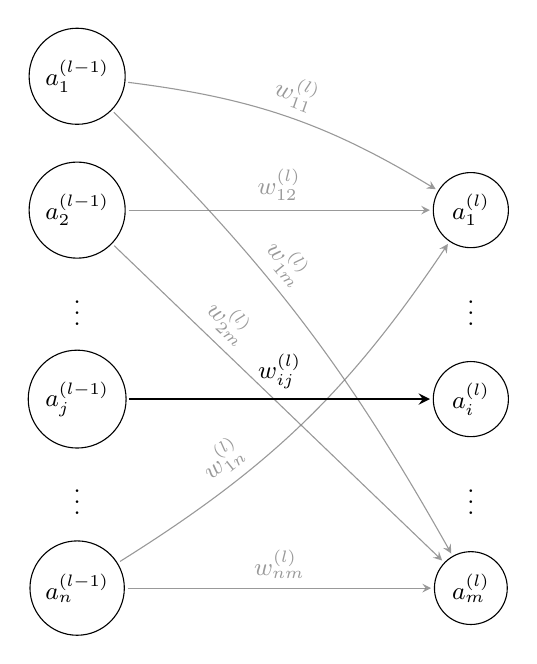
\begin{tikzpicture}[>=stealth, every node/.style={font=\small}, every path/.style={->, shorten >=1pt, shorten <=1pt}]
                % Source layer (l-1) with ellipses to indicate generality
                \node[circle, draw] (N1) at (0,0.5)    {$a_{1}^{(l-1)}$};
                \node[circle, draw] (N2) at (0,-1.2) {$a_{2}^{(l-1)}$};
                \node at (0,-2.4) {$\vdots$};
                \node[circle, draw] (Nj) at (0,-3.6) {$a_{j}^{(l-1)}$};
                \node at (0,-4.8) {$\vdots$};
                \node[circle, draw] (Nn) at (0,-6) {$a_{n}^{(l-1)}$};

                % Target layer l with ellipses
                \node[circle, draw, minimum size=0.9cm] (M1) at (5,-1.2) {$a_{1}^{(l)}$};
                \node at (5,-2.4) {$\vdots$};
                \node[circle, draw, minimum size=0.9cm] (Mi) at (5,-3.6) {$a_{i}^{(l)}$};
                \node at (5,-4.8) {$\vdots$};
                \node[circle, draw, minimum size=0.9cm] (Mm) at (5,-6) {$a_{m}^{(l)}$};

                % faint generic connections to show full connectivity
                \draw[->, gray, opacity=0.8, bend left=12]  (N1) to node[sloped, above] {$w_{11}^{(l)}$} (M1);
                \draw[->, gray, opacity=0.8]                  (N2) to node[sloped, above] {$w_{12}^{(l)}$} (M1);
                \draw[->, gray, opacity=0.8, bend right=12]  (Nn) to node[pos=0.3, sloped, above] {$w_{1n}^{(l)}$} (M1);

                \draw[->, gray, opacity=0.8, bend left=8]   (N1) to node[pos=0.4, sloped, above] {$w_{1m}^{(l)}$} (Mm);
                \draw[->, gray, opacity=0.8]                  (N2) to node[pos=0.30, sloped, above] {$w_{2m}^{(l)}$} (Mm);
                \draw[->, gray, opacity=0.8]   (Nn) to node[sloped, above] {$w_{nm}^{(l)}$} (Mm);

                % highlighted connection showing the general index i,j
                \draw[->, thick] (Nj) to node[midway, above] {$\;w_{ij}^{(l)}\;$} (Mi);
            \end{tikzpicture}
        \end{center}
        \item Each $b_{i}^{(l)}$ is the bias for neuron $i$ in layer $l$.
    \end{itemize}
    The \textbf{gradient} $\nabla E(w)$ then contains the partial derivatives of the loss function with respect to \textbf{each individual weight and bias} in the network:
    \begin{equation}
        \nabla E(w) = \left\{
            \dfrac{\partial \, E}{\partial \, w_{ij}^{(l)}} , \,
            \dfrac{\partial \, E}{\partial \, b_{i}^{(l)}}
        \right\}
    \end{equation}
    The \textbf{core learning rule} still applies, but now we update \textbf{each weight and bias} individually:
    \begin{equation}
        w_{ij}^{(l)} \leftarrow w_{ij}^{(l)} - \eta \,\dfrac{\partial \, E}{\partial \, w_{ij}^{(l)}} \quad \text{and} \quad
        b_{i}^{(l)} \leftarrow b_{i}^{(l)} - \eta \,\dfrac{\partial \, E}{\partial \, b_{i}^{(l)}}
    \end{equation}
    This is how \textbf{gradient descent} is applied in the context of training neural networks.
\end{definitionbox}

\begin{flushleft}
    \textcolor{Green3}{\faIcon{tools} \textbf{How it works (intuitively)}}
\end{flushleft}
Intuitively, gradient descent works as follows:
\begin{enumerate}
    \item Start from an \textbf{initial guess} for the weights $w_{0}$ (often random).
    \item Compute the \textbf{gradient} $\nabla E(w_{0})$ of the loss function at the current weights:
    \begin{equation*}
        \nabla E(w_{0}) = \begin{bmatrix}
            \dfrac{\partial \, E}{\partial \, w_{1}} \\[1.2em]
            \dfrac{\partial \, E}{\partial \, w_{2}} \\[1.2em]
            \vdots \\
            \dfrac{\partial \, E}{\partial \, w_{d}}
        \end{bmatrix}_{w = w_{0}}
    \end{equation*}

    \item Do a step \textbf{against} that gradient to update the weights using the \textbf{core learning rule}:
    \begin{equation*}
        w_{k+1} = w_{k} - \eta \,\nabla E(w_{k})
        \quad \Rightarrow \quad
        w_{1} = w_{0} - \eta \,\nabla E(w_{0})
    \end{equation*}
    Then, the new weights $w_{1}$ should yield a \textbf{lower loss} $E(w_{1}) < E(w_{0})$. If we were on a neural network, we would update \textbf{all weights and biases} similarly:
    \begin{equation*}
        w_{ij}^{(l)} \leftarrow w_{ij}^{(l)} - \eta \,\dfrac{\partial \, E}{\partial \, w_{ij}^{(l)}}
        \quad , \quad
        b_{i}^{(l)} \leftarrow b_{i}^{(l)} - \eta \,\dfrac{\partial \, E}{\partial \, b_{i}^{(l)}}
    \end{equation*}
    \item Repeat until: the gradient becomes small (close to zero), or we reach a maximum number of iterations.
\end{enumerate}

\noindent
\textcolor{Green3}{\faIcon{\speedIcon} \textbf{Convergence Speed}} \textbf{and} \textcolor{Red2}{\faIcon{exclamation-triangle} \textbf{False Positives}}. The speed at which gradient descent converges to the minimum depends on:
\begin{itemize}
    \item The \textbf{shape} of the loss function (e.g., steepness, curvature). It strongly affects how gradient descent behaves:
    \begin{itemize}
        \item \textbf{Convex surface} (like a bowl): Gradient descent always converges there (since there is a \textbf{single global minimum}). However, if $\eta$ is too large, it may oscillate around the minimum.

        \item \textbf{Non-convex surface} (like many hills and valleys): There may be \textbf{multiple local minima} and \textbf{saddle points}. Gradient descent might: 
        \begin{itemize}
            \item[\textcolor{Red2}{\faIcon{exclamation-triangle}}] Get stuck in a \textbf{local minimum} (the derivative is zero, but it is not the global optimum).
            \item Oscillate in flat regions.
            \item Move very slowly along narrow valleys.
        \end{itemize}
    \end{itemize}


    \item The \textbf{learning rate} $\eta$.

    \textcolor{Green3}{\faIcon[regular]{lightbulb}} The \textbf{learning rate} $\eta$ is crucial: it controls \textbf{how big a step} we take each iteration.
    \begin{itemize}
        \item $\eta$ too \textbf{small} $\rightarrow$ \textbf{Learning is very slow} because we take tiny steps (many iterations needed).
        \item $\eta$ too \textbf{large} $\rightarrow$ \textbf{May overshoot the minimum} and even diverge (loss increases instead of decreasing).
        \item Choosing a good $\eta$ is often done via \textbf{experimentation} or using techniques. However, if $\eta$ is chosen well, gradient descent can efficiently find a good set of weights that minimize the loss function.
    \end{itemize}
    Don't worry if this seems abstract now; we'll later learn that \textbf{adaptive optimizers} (like \emph{\textbf{momentum}}, \emph{\textbf{Adam}}, etc.) are more robust ways to handle this.


    \item The \textbf{initial weights} $w_{0}$. In \textbf{convex} functions (like a parabola), there is a global minimum, and \emph{gradient descent} will converge to it. In \textbf{non-convex} functions (like many neural network loss landscapes), there may be multiple local minima, and gradient descent may converge to one of them depending on the starting point. So in practice, we \hl{often run gradient descent multiple times with different initial weights to find a good solution}.
\end{itemize}

\begin{figure}[!htp]
    \centering
    \includegraphics[width=.8\textwidth]{img/learning-and-optimization/convex-bowl-contour.pdf}
    \caption{Example of a \textbf{convex quadratic surface} (bowl-shaped). The contour lines (ellipses) represent levels of constant error $E\left(w_{1}, w_{2}\right)$. There is a \textbf{single global minimum} at the center of the bowl ($w_{1}^{*} = 2, w_{2}^{*} = -1$), and outer ellipses represent higher error values. This is the ideal scenario for gradient descent, as it will always converge to the global minimum regardless of the starting point (similar to Figure \ref{fig:error-geometric-interpretation-1}, page \pageref{fig:error-geometric-interpretation-1}).}
    \label{fig:convex-bowl-contour}
\end{figure}

\begin{figure}[!htp]
    \centering
    \includegraphics[width=\textwidth]{img/learning-and-optimization/non-convex-wavy-contour.pdf}
    \caption{Example of a \textbf{non-convex surface} with multiple local minima and saddle points. The loss function $E\left(w_{1}, w_{2}\right)$ has two components: (1) the \textbf{quadratic bowl} that pushes weights toward the global minimum, and (2) the \textbf{sinusoidal term} that introduces \emph{oscillations} in the surface. Those oscillations create \textbf{small waves} (bumps and dips). Each dip (a small valley) is a \emph{local minimum}, and each bump is a \emph{local maximum} or ridge. This is what happens in \textbf{non-linear models} like deep neural networks, where the composition of many layers and activations makes the error surface very complex (and non-convex). There are thousands or millions of such local minima, making optimization challenging. Gradient descent may get trapped in one of these local minima instead of finding the global minimum. However, in practice, many local minima have \textbf{similar performance}, so this isn't always bad.}
    \label{fig:non-convex-surface-contour}
\end{figure}
    \subsubsection{Backpropagation (Conceptual Introduction)}\label{sec:backpropagation-conceptual-introduction}

\begin{flushleft}
    \textcolor{Green3}{\faIcon{question-circle} \textbf{Why Backpropagation exists?}}
\end{flushleft}
The \textbf{problem} we face is computational:
\begin{itemize}
    \item Gradient descent (page \pageref{sec:gradient-descent-basics}) at each iteration requires the computation of \textbf{all partial derivatives} of the loss function $E$ with respect to \textbf{all weights and biases} in the network. Formally, we need to compute (introduced in section \ref{sec:gradient-descent-basics}, page \pageref{eq:gradient-neural-network}):
    \begin{equation*}
        \nabla E(w) = \left\{
            \dfrac{\partial \, E}{\partial \, w_{ij}^{(l)}} , \,
            \dfrac{\partial \, E}{\partial \, b_{i}^{(l)}}
        \right\}
    \end{equation*}
    \item In a network with thousands of weights, each weight influences the output \emph{indirectly} through multiple layers.
\end{itemize}
Computing those derivatives by brute force (finite differences or manual application of the chain rule) would be \textbf{computationally expensive} and \textbf{inefficient}. We need a more efficient way to compute these gradients.

\highspace
\begin{flushleft}
    \textcolor{Green3}{\faIcon[regular]{lightbulb} \textbf{Backpropagation Concept}}
\end{flushleft}
\definition{Backpropagation} (or \textbf{backward propagation of errors}) is an efficient \textbf{algorithm} used to \textbf{compute the gradients} of the loss function with respect to all weights and biases \textbf{in a neural network}. It leverages the \textbf{chain rule of calculus} in a systematic, efficient way to reuse computations and propagate errors backward through the network. It is analogous to hashmaps in programming, where intermediate results are stored and reused to avoid redundant calculations.

\highspace
\begin{remarkbox}[: The Chain Rule]\label{box:chain-rule}
    The \definition{Chain Rule} is a fundamental rule in calculus used to compute the derivative of a composite function.

    Suppose we have a \textbf{function inside another function}:
    \begin{equation*}
        y = f\left(g(x)\right)
    \end{equation*}
    We want to know how $y$ changes when we slightly change $x$. In other words, we want to find the derivative $\dfrac{\partial y}{\partial x}$. The chain rule tells us that we can break this down into two parts:
    \begin{equation}
        \dfrac{\partial y}{\partial x} = \dfrac{\partial y}{\partial g} \cdot \dfrac{\partial g}{\partial x}
    \end{equation}
    This means that to find out how $y$ changes with respect to $x$, we first find out how $y$ changes with respect to $g$ (the inner function), and then multiply that by how $g$ changes with respect to $x$. It's literally ``follow the chain'' of dependencies.

    Let's see a quick example. Let's say:
    \begin{equation*}
        y = f\left(g(x)\right) = \left(2x + 3\right)^{2}
    \end{equation*}
    We can identify:
    \begin{itemize}
        \item Inner function: $g(x) = 2x + 3$
        \item Outer function: $f(g) = g^{2}$
    \end{itemize}
    Now, we compute the derivatives:
    \begin{itemize}
        \item $\dfrac{\partial f}{\partial g} \left(g^{2}\right) = 2g$
        \item $\dfrac{\partial g}{\partial x} \left(2x + 3\right) = 2$
    \end{itemize}
    Now, applying the chain rule:
    \begin{equation*}
        \dfrac{\partial y}{\partial x} = \dfrac{\partial f}{\partial g} \cdot \dfrac{\partial g}{\partial x} = 2g \cdot 2 = 4g
    \end{equation*}
    Finally, substituting back $g(x)$:
    \begin{equation*}
        \dfrac{\partial y}{\partial x} = 4(2x + 3) = 8x + 12
    \end{equation*}
\end{remarkbox}

\highspace
Conceptually, Backpropagation works during the training phase of a neural network. \textbf{During training phase}, there are \textbf{two complementary flows} of information:
\begin{itemize}
    \item \important{Forward Pass} (Input $\to$ Output): The purpose is to \textbf{measure how good the current weights are at predicting the target outputs}. The input data is passed through the network layer by layer to compute the output. During this phase, the activations of each neuron are computed and stored for later use. Formally, compute predictions $y(x;w)$ for input $x$ and weights $w$, and save intermediate activations $a^{(l)}$ for each layer $l$. Here, $a^{(l)}$ represents the activations at layer $l$:
    \begin{equation*}
        a^{(l)} = f\left( W^{(l)} a^{(l-1)} + b^{(l)} \right) = f(z^{(l)})
    \end{equation*}
    where $f$ is the activation function, $W^{(l)}$ are the weights, and $b^{(l)}$ are the biases at layer $l$.

    \item \important{Backward Pass} (Output $\to$ Input): The purpose is to \textbf{know how to change weights to reduce the loss}. The error (the difference between the predicted output and the actual target) is propagated backward through the network. During this phase, the gradients of the loss function with respect to each weight and bias are computed using the chain rule, utilizing the stored activations from the forward pass. Formally, compute gradients $\dfrac{\partial E}{\partial w_{ij}^{(l)}}$ and $\dfrac{\partial E}{\partial b_{i}^{(l)}}$ for all weights and biases using the chain rule. The stored activations $a^{(l)}$ are used to compute these gradients efficiently.
\end{itemize}
Hence the name \textbf{backpropagation}: the error is propagated backward through the network to compute gradients efficiently. In the next pages, we will see a detailed example of how backpropagation works step by step. Formally deriving the backpropagation equations will be covered in later sections.

\highspace
\begin{examplebox}[: Numerical Example of Backpropagation Concept]
    We'll train a \textbf{1-hidden-layer neural network} to learn the function $y = x$ for one input sample $x=1$ and target $t=0.5$. Visually, the network looks like this:
    \begin{center}
        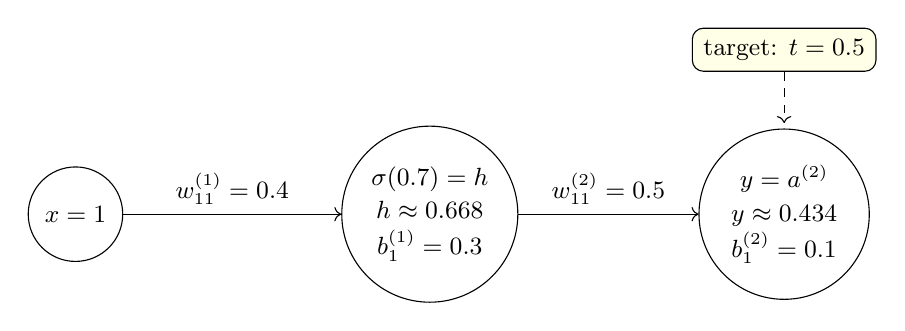
\begin{tikzpicture}[->, every node/.style={font=\small}]
            % nodes (increased sizes and spacing)
            \node[circle,draw,minimum size=12mm] (in) at (0,0) {$x=1$};
            \node[circle,draw,minimum size=20mm,align=center] (h)  at (4.5,0) {$\sigma(0.7) = h$\\[1pt] $h\approx0.668$\\[2pt]\small $b_{1}^{(1)}=0.3$};
            \node[circle,draw,minimum size=20mm,align=center] (out) at (9,0) {$y=a^{(2)}$\\[1pt] $y\approx0.434$\\[2pt]\small $b_{1}^{(2)}=0.1$};

            % target node placed above the output node (inside the picture)
            \node[draw,rectangle,rounded corners,fill=yellow!10,inner sep=4pt] (target) at ($(out.north)+(0,1.0)$) {target: $t=0.5$};

            % connections with weight labels
            \draw (in) -- node[above] {$w_{11}^{(1)}=0.4$} (h);
            \draw (h)  -- node[above] {$w_{11}^{(2)}=0.5$} (out);

            % dashed vertical arrow from target down to output (avoids overlapping)
            \draw[->, dashed, shorten >=2pt] (target.south) to[bend right=0] (out.north);
        \end{tikzpicture}
    \end{center}
    The network architecture is as follows:
    \begin{itemize}
        \item Input layer: 1 neuron, with notation $a^{(0)} = x = 1$.
        \item Hidden layer: 1 neuron, with a sigmoid activation function:
        \begin{equation*}
            g^{(1)}(a) = \sigma(a) = \dfrac{1}{1+e^{-a}}
        \end{equation*}
        \item Output layer: 1 neuron, with notation $y = w_{2} \cdot h + b_{2}$. Where $y$ is the output, $w_{2}$ is the weight connecting hidden to output layer, and $b_{2}$ is the bias of the output layer. The activation function is linear:
        \begin{equation*}
            g^{(2)}(a) = a
        \end{equation*}
    \end{itemize}
    The weights and biases are initialized as follows (randomly chosen for this example):
    \begin{itemize}
        \item $w_{11}^{(1)} = 0.4$ (weight from input to hidden layer)
        \item $b_{1}^{(1)} = 0.3$ (bias of hidden layer)
        \item $w_{11}^{(2)} = 0.5$ (weight from hidden to output layer)
        \item $b_{1}^{(2)} = 0.1$ (bias of output layer)
    \end{itemize}
    The learning rate $\eta$ is set to $0.1$.

    \highspace
    \important{Backpropagation Step 1: Forward Pass.} In this step, we compute the activations of the hidden and output layers given the input $a^{(0)} = x = 1$.
    \begin{enumerate}
        \item \textbf{Compute hidden layer activation} (net input). The neuron has the index $i=1$ in layer $l=1$ since it's the first hidden layer (equation \ref{eq:net-input}, page \pageref{eq:net-input}):
        \begin{equation*}
            a_{1}^{(1)} = w_{11}^{(1)} \cdot a^{(0)} + b_{1}^{(1)} = 0.4 \cdot 1 + 0.3 = 0.7
        \end{equation*}
        The $a_{1}^{(1)}$ calculated above is the weighted sum before activation. Now, this value is passed through the sigmoid activation function:
        \begin{equation*}
            h = g^{(1)}\left(a_{1}^{(1)}\right) = g^{(1)}\left(0.7\right) = \sigma(0.7) = \dfrac{1}{1 + e^{-0.7}} \approx 0.668
        \end{equation*}
        \item \textbf{Compute output layer activation}. Again, using equation \ref{eq:net-input} (page \pageref{eq:net-input}), we compute the net input to the output neuron:
        \begin{equation*}
            a_{1}^{(2)} = w_{11}^{(2)} \cdot h + b_{1}^{(2)} = 0.5 \cdot 0.668 + 0.1 \approx 0.434
        \end{equation*}
        But now, Since the output layer uses a linear activation function, the output is:
        \begin{equation*}
            y = g^{(2)}(a_{1}^{(2)}) = a_{1}^{(2)} \approx 0.434
        \end{equation*}
        \item \textbf{Compute the error}. The predicted output from the forward pass is $y \approx 0.434$. The error can now be computed using the target $t=0.5$. For example, using Mean Squared Error (MSE):
        \begin{equation*}
            E = \dfrac{1}{2} \left(t - y\right)^{2} = \dfrac{1}{2} \left(0.5 - 0.434\right)^{2} \approx 0.0022
        \end{equation*}
        This error quantifies how far the network's prediction is from the target.
    \end{enumerate}
    At the end of this step, we have stored (cached) some intermediate values needed for the backward pass:
    \begin{itemize}
        \item \textbf{Input activation}: $a^{(0)} = 1$
        \item \textbf{Linear combo to hidden layer}: $a_{1}^{(1)} = w_{11}^{(1)} \cdot a^{(0)} + b_{1}^{(1)} = 0.7$
        \item \textbf{Hidden layer activation}: $h = g^{(1)}\left(a_{1}^{(1)}\right) = \sigma\left(0.7\right) \approx 0.668$
        \item \textbf{Linear combo to output layer}: $a_{1}^{(2)} = w_{11}^{(2)} \cdot h + b_{1}^{(2)} \approx 0.434$
        \item \textbf{Output activation (identity)}: $y = g^{(2)}\left(a_{1}^{(2)}\right) \approx 0.434$
        \item \textbf{Error}: $E \approx 0.0022$
    \end{itemize}
    \important{Backpropagation Step 2: Backward Pass.} In this step, we compute the gradients of the loss function with respect to each weight and bias using backpropagation. We use the Mean Squared Error (MSE, page \pageref{box:mse}) loss function:
    \begin{equation*}
        E = \dfrac{1}{2} \left(t - y\right)^{2}
    \end{equation*}
    Where $t$ is the target output ($t=0.5$) and $y$ is the predicted output from the forward pass ($y \approx 0.434$). We will compute the gradients layer by layer, starting from the output layer and moving backward to the hidden layer. Also, we will \textbf{denote the error term for each layer as} $\delta^{(l)}$ and we propagate it backward through the network (using the cached values from the forward pass!). Simply put, we need to find $\nabla E(w)$:
    \begin{equation*}
        \nabla E(w) = \left\{
            \dfrac{\partial \, E}{\partial \, w_{ij}^{(l)}} , \,
            \dfrac{\partial \, E}{\partial \, b_{i}^{(l)}}
        \right\} = \left\{
            \dfrac{\partial \, E}{\partial \, w_{11}^{(2)}}, \,
            \dfrac{\partial \, E}{\partial \, b_{1}^{(2)}}, \,
            \dfrac{\partial \, E}{\partial \, w_{11}^{(1)}}, \,
            \dfrac{\partial \, E}{\partial \, b_{1}^{(1)}}
        \right\}
    \end{equation*}
    Where:
    \begin{equation*}
        \dfrac{\partial \, E}{\partial \, w_{ij}^{(l)}} = \dfrac{\partial \, E}{\partial \, y} \cdot \dfrac{\partial \, y}{\partial \, a_{i}^{(l)}} \cdot \dfrac{\partial \, a_{i}^{(l)}}{\partial \, w_{ij}^{(l)}}
        \qquad
        \dfrac{\partial \, E}{\partial \, b_{i}^{(l)}} = \dfrac{\partial \, E}{\partial \, y} \cdot \dfrac{\partial \, y}{\partial \, a_{i}^{(l)}} \cdot \dfrac{\partial \, a_{i}^{(l)}}{\partial \, b_{i}^{(l)}}
    \end{equation*}
    However, to avoid recomputing terms, we define the error term $\delta^{(l)}$ for layer $l$ as:
    \begin{equation*}
        \delta^{(l)} = \dfrac{\partial E}{\partial a_{i}^{(l)}} = \dfrac{\partial E}{\partial y} \cdot \dfrac{\partial y}{\partial a_{i}^{(l)}}
    \end{equation*}
    This allows us to express the gradients more compactly:
    \begin{equation*}
        \dfrac{\partial E}{\partial w_{ij}^{(l)}} = \delta^{(l)} \cdot a_{j}^{(l-1)}
        \qquad
        \dfrac{\partial E}{\partial b_{i}^{(l)}} = \delta^{(l)}
    \end{equation*}
    These equations may be unfamiliar now, but they will make sense in future sections when we derive them formally.
    For now, let's treat them as given formulas for computing the gradients using the error terms $\delta^{(l)}$.

    Now, we compute $\delta^{(l)}$ for each layer starting from the output layer and moving backward to the hidden layer.
    The steps are as follows:
    \begin{enumerate}
        \item \textbf{Compute the error at the output layer}:
        \begin{align*}
            \dfrac{\partial \, E}{\partial \, b_{i}^{(l)}} = \dfrac{\partial E}{\partial b_{1}^{(2)}} = \delta^{(2)} & = \dfrac{\partial E}{\partial y} \cdot \dfrac{\partial y}{\partial a_{1}^{(2)}} \\[.3em]
                                                                                                                     & = \dfrac{\partial }{\partial y} \left( \dfrac{1}{2} (t - y)^{2} \right) \cdot 1 \\[.3em]
                                                                                                                     & = -(t - y) \cdot 1 \\
                                                                                                                     & = - (0.5 - 0.434) = -0.066
        \end{align*}
        It represents how much the output $y$ deviates from the target $t$. Here we used the output activation function value $y$ from the \textbf{cached values}.
        \item \textbf{Compute gradients for weights and biases in the output layer}:
        \begin{equation*}
            \underbrace{\dfrac{\partial E}{\partial w_{11}^{(2)}}}_{\dfrac{\partial \, E}{\partial \, w_{ij}^{(l)}}} = \delta^{(2)} \cdot \underbrace{a_{1}^{(1)}}_{a_{j}^{(l-1)}} = \delta^{(2)} \cdot h \approx -0.066 \cdot 0.668 \approx -0.044
        \end{equation*}
        It shows how much the weight $w_{11}^{(2)}$ should be adjusted to reduce the error. It will be used to update the weight during the optimization step. Again, we used the hidden layer activation ($h \approx 0.668$) from the \textbf{cached values}. Now, also compute the gradient for the bias that is obtained directly from the previously step (also \textbf{cached}):
        \begin{equation*}
            \dfrac{\partial \, E}{\partial \, b_{i}^{(l)}} = \dfrac{\partial E}{\partial b_{1}^{(2)}} = \delta^{(2)} \approx -0.066
        \end{equation*}
        \item Compute the error at the hidden layer:
        \begin{equation*}
            \delta^{(1)} = \delta^{(2)} \cdot w_{11}^{(2)} \cdot g'^{(1)}\left(a_{1}^{(1)}\right)
        \end{equation*}
        where $g'^{(1)}(a)$ is the derivative of the sigmoid function:
        \begin{equation*}
            g'^{(1)}(a) = \sigma(a) \cdot \left(1 - \sigma(a)\right)
        \end{equation*}
        Thus,
        \begin{equation*}
            g'^{(1)}(0.7) = \sigma(0.7) \cdot \left(1 - \sigma(0.7)\right) \approx 0.668 \cdot \left(1 - 0.668\right) \approx 0.222
        \end{equation*}
        Where we used the \textbf{cached values} of the activation of the hidden layer $\sigma(0.7) \approx 0.668$ from the forward pass. Therefore,
        \begin{equation*}
            \delta^{(1)} \approx -0.066 \cdot 0.5 \cdot 0.222 \approx -0.0073
        \end{equation*}
        \item Compute gradients for weights and biases in the hidden layer:
        \begin{equation*}
            \dfrac{\partial E}{\partial w_{11}^{(1)}} = \delta^{(1)} \cdot a^{(0)} \approx -0.0073 \cdot 1 \approx -0.0073
        \end{equation*}
        \begin{equation*}
            \dfrac{\partial E}{\partial b_{1}^{(1)}} = \delta^{(1)} \approx -0.0073
        \end{equation*}
    \end{enumerate}
    \textbf{Step 3: Update Weights and Biases.} Finally, we update the weights and biases using the computed gradients and the learning rate $\eta = 0.1$ (all the gradients are \textbf{cached} from the backward pass):
    \begin{itemize}
        \item Update weight from hidden to output layer:
        \begin{equation*}
            w_{11}^{(2)} \leftarrow w_{11}^{(2)} - \eta \cdot \dfrac{\partial E}{\partial w_{11}^{(2)}} \approx 0.5 - 0.1 \cdot (-0.044) \approx 0.5044
        \end{equation*}
        \item Update bias of output layer:
        \begin{equation*}
            b_{1}^{(2)} \leftarrow b_{1}^{(2)} - \eta \cdot \dfrac{\partial E}{\partial b_{1}^{(2)}} \approx 0.1 - 0.1 \cdot (-0.066) \approx 0.1066
        \end{equation*}
        \item Update weight from input to hidden layer:
        \begin{equation*}
            w_{11}^{(1)} \leftarrow w_{11}^{(1)} - \eta \cdot \dfrac{\partial E}{\partial w_{11}^{(1)}} \approx 0.4 - 0.1 \cdot (-0.0073) \approx 0.40073
        \end{equation*}
        \item Update bias of hidden layer:
        \begin{equation*}
            b_{1}^{(1)} \leftarrow b_{1}^{(1)} - \eta \cdot \dfrac{\partial E}{\partial b_{1}^{(1)}} \approx 0.3 - 0.1 \cdot (-0.0073) \approx 0.30073
        \end{equation*}
    \end{itemize}
    After this single iteration of forward and backward passes, the weights and biases have been updated to better approximate the target function $y = x$ for the input $x=1$. Repeating this process over many iterations and samples will allow the network to learn the desired mapping.
\end{examplebox}
    \subsection{Maximum Likelihood Estimation (MLE)}\label{sec:maximum-likelihood-estimation}

In the previous sections, we discussed how to \emph{compute} gradients (backpropagation) and \emph{optimize} weights (gradient descent) in neural networks. But \textbf{why} do we minimize a loss function in the first place? What's the \textbf{statistical justification} for this approach? Is there a \textbf{probabilistic interpretation} of learning in neural networks? And why is it important?

\highspace
We've already seen that when we train a neural network, we \emph{minimize a loss function} $E(w)$ (page \pageref{eq:optimal-weights}). MLE gives a \textbf{statistical justification} for that loss: it's equivalent to \textbf{maximizing the probability} of observing our data given the model parameters. In other words, \textbf{MLE turns learning into a probability problem}.

\highspace
\begin{definitionbox}[: Maximum Likelihood Estimation (MLE)]
    Let our model have parameters $\theta$ (or $w$ in neural networks), and our dataset be:
    \begin{equation*}
        \mathcal{D} = \left\{ x_{1}, x_{2}, \ldots, x_{N} \right\}
    \end{equation*}
    We assume that each data point is drawn from a probability distribution that depends on those parameters:
    \begin{equation*}
        p\left(x_{n} \, \mid \, \theta\right)
    \end{equation*}
    If all samples are \textbf{i.i.d.} (independent and identically distributed) then the probability of the entire dataset is:
    \begin{equation*}
        p\left(\mathcal{D} \, \mid \, \theta\right) = \displaystyle\prod_{n=1}^{N} p\left(x_{n} \, \mid \, \theta\right)
    \end{equation*}
    This is called the \textbf{likelihood function}:
    \begin{equation}
        L\left(\theta\right) = p\left(\mathcal{D} \, \mid \, \theta\right) = \displaystyle\prod_{n=1}^{N} p\left(x_{n} \, \mid \, \theta\right)
    \end{equation}
    Then the \definition{Maximum Likelihood Estimation (MLE)} is the value of $\theta$ that maximizes this likelihood:
    \begin{equation}
        \hat{\theta}_{\text{MLE}} = \arg\max_{\theta} L\left(\theta\right) = \arg\max_{\theta} p\left(\mathcal{D} \, \mid \, \theta\right)
    \end{equation}
    In practice, we often maximize the \textbf{log-likelihood} instead:
    \begin{equation}
        \hat{\theta}_{\text{MLE}} = \arg\max_{\theta} \log L\left(\theta\right) = \arg\max_{\theta} \log p\left(\mathcal{D} \, \mid \, \theta\right)
    \end{equation}
    Because the logarithm is a monotonic function, maximizing the log-likelihood is equivalent to maximizing the likelihood itself. Also, the logarithm allows us to turn products into sums, which are easier to work with.
\end{definitionbox}

\highspace
\begin{flushleft}
    \textcolor{Green3}{\faIcon{question-circle} \textbf{What does i.i.d. mean?}}\label{def:iid}
\end{flushleft}
The acronym \definitionWithSpecificIndex{i.i.d.}{Independent and Identically Distributed (i.i.d.)}{} stands for \emph{independent and identically distributed}. It's a \textbf{fundamental assumption} in statistics that simplifies how we model data. When we say that our samples are i.i.d., we mean two things:
\begin{enumerate}
    \item \important{Independent}. Each observation (data point) does \textbf{not depend} on the others. Formally:
    \begin{equation*}
        p\left(x_{1}, x_{2}, \dots, x_{N}\right) = \displaystyle\prod_{n=1}^{N} p\left(x_{n}\right)
    \end{equation*}
    So, knowing $x_{1}$ tells us nothing about $x_{2}$, and so on. Each is separate, independent draw from the underlying process. For example, if we toss a coin 10 times, each toss is independent of the others, assuming the coin is fair and the tosses don't influence each other.

    \item \important{Identically Distributed}. All samples come from the \textbf{same probability distribution}. Formally:
    \begin{equation*}
        x_{n} \sim p\left(x \mid \theta\right) \quad \forall n
    \end{equation*}
    This means they are generated by the \textbf{same model parameters} ($\theta$) (e.g., same mean and variance in a Gaussian). For example, each coin toss has the same probability ($P(\text{Head}) = 0.5$).
\end{enumerate}
So, when we say:
\begin{equation*}
    x_{1}, x_{2}, \ldots, x_{N} \overset{\text{are i.i.d.}}{\sim} p\left(x \mid \theta\right)
\end{equation*}
We mean that each sample $x_{n}$ is an independent draw from the \textbf{same} distribution underlying probability parameterized by $\theta$. This is the \textbf{standard assumption} when deriving the Likelihood:
\begin{equation*}
    p\left(\mathcal{D} \, \mid \, \theta\right) = \displaystyle\prod_{n=1}^{N} p\left(x_{n} \, \mid \, \theta\right)
\end{equation*}
Without the i.i.d. assumption, we couldn't factor the joint probability into a product of individual probabilities, making the analysis much more complex.

\highspace
\begin{flushleft}
    \textcolor{Green3}{\faIcon[regular]{lightbulb} \textbf{Core Idea of MLE}}
\end{flushleft}
The core idea of MLE is to find the parameter values that make the \textbf{observed data most probable} under our assumed statistical model. By maximizing the likelihood function, we identify the parameters that best explain the data we have collected. Let's illustrate this with a simple example.

\highspace
Imagine a \textbf{Gaussian distribution} (bell curve) centered around some unknown true mean $\hat{\mu}$. Each black point below the curve represents one \textbf{sample} (observation): $x_{1}, x_{2}, \ldots, x_{N}$. These samples:
\begin{itemize}
    \item Come from the \textbf{same distribution} $\mathcal{N}\left(\mu, \sigma^{2}\right)$, so they are \textbf{identically distributed}. It means they share the same mean $\mu$ and variance $\sigma^{2}$.
    \item Are drawn \textbf{independently} from each other, so they are \textbf{independent}.
\end{itemize}
If we were to repeat the sampling many times, we'd get different sets of samples, but all coming from \emph{the same bell curve}.

\newpage

\begin{figure}[!htp]
    \centering
    \includegraphics[width=\textwidth]{img/maximum-likelihood-estimation/gaussian-samples.pdf}
\end{figure}

\noindent
Now, MLE asks: ``\emph{which value of $\mu$ would make these observed points most likely under the Gaussian model?}'' If we shift the curve too far left or right, the points no longer lie near its center, reducing their likelihood. The ``best'' $\mu$ is the one centering the curve on the data cloud, called $\hat{\mu}_{\text{MLE}}$. This $\hat{\mu}_{\text{MLE}}$ is the \textbf{Maximum Likelihood Estimate} of the mean.

\highspace
Let's derive the MLE for the mean of a Gaussian distribution step-by-step.
\begin{enumerate}
    \item \important{Model assumption}. We assume our data points are i.i.d. samples from a Gaussian distribution:
    \begin{equation*}
        x_1, x_2, \dots, x_N \sim \mathcal{N}(\mu, \sigma^2)
    \end{equation*}
    Where $\sigma^2$ is known, and $\mu$ is the parameter we want to estimate. Each point has probability density:
    \begin{equation*}
        p\left(x_n \mid \mu, \sigma^{2}\right) = \dfrac{1}{\sqrt{2 \pi \sigma^2}} \exp\left(-\dfrac{\left(x_n - \mu\right)^2}{2 \sigma^2}\right)
    \end{equation*}
    The \textbf{probability density} is a function that describes the likelihood of a random variable taking on a specific value. For continuous variables, it indicates how dense the probability is around that value.

    \item \important{Likelihood of the dataset}. The likelihood of the entire dataset, assuming i.i.d. samples, is:
    \begin{equation*}
        L\left(\mu\right) = p\left(\mathcal{D} \mid \mu, \sigma^{2}\right) = \prod_{n=1}^{N} p\left(x_n \mid \mu, \sigma^{2}\right)
    \end{equation*}

    \item \important{Log-likelihood}. We take the logarithm of the likelihood to simplify calculations:
    \begin{equation*}
        \log \ell\left(\mu\right) = -\dfrac{N}{2}\log\left(2 \pi \sigma^{2}\right) - \dfrac{1}{2 \sigma^{2}} \sum_{n=1}^{N} \left(x_n - \mu\right)^2
    \end{equation*}

    \important{Derivative with respect to $\mu$}. We differentiate the log-likelihood with respect to $\mu$ because we want to find the value of $\mu$ that maximizes it (and the gradient tells us where the maximum is):
    \begin{align*}
        \dfrac{\partial \ell}{\partial \mu} = & -\dfrac{1}{2\sigma^{2}} \cdot \dfrac{\partial}{\partial \mu} \sum_{n=1}^{N} \left(x_n - \mu\right)^{2} \\[.3em]
        = & -\dfrac{1}{2\sigma^{2}} \cdot \sum_{n=1}^{N} 2\left(\mu - x_n\right) \\[.3em]
        \Rightarrow & \, \dfrac{1}{\sigma^{2}} \cdot \displaystyle \sum_{n=1}^{N} \left(x_n - \mu\right)
    \end{align*}

    \item \important{Set derivative to zero}. To find the maximum, we set the derivative equal to zero and solve for $\mu$, because at the maximum point, the slope of the function is zero:
    \begin{align*}
        0 = & \, \dfrac{1}{\sigma^{2}} \cdot \displaystyle \sum_{n=1}^{N} \left(x_n - \mu\right) \\[.3em]
        \Rightarrow & \, \sum_{n=1}^{N} x_n - N \mu = 0 \\[.3em]
        \Rightarrow & \, N \mu = \sum_{n=1}^{N} x_n \\[.3em]
        \Rightarrow & \, \mu = \dfrac{1}{N} \cdot \sum_{n=1}^{N} x_n
    \end{align*}
    Thus, the MLE for the mean of a Gaussian distribution is the \textbf{sample mean}:
    \begin{equation}
        \hat{\mu}_{\text{MLE}} = \dfrac{1}{N} \cdot \sum_{n=1}^{N} x_n
    \end{equation}
\end{enumerate}
This derivation shows \hl{how MLE provides a principled way to estimate model parameters by maximizing the likelihood of the observed data}. In this case, it leads us to the intuitive result that the \hl{best estimate for the mean of a Gaussian is simply the average of the observed samples}. In simple terms, Gaussian is the geometric intuition behind the MLE of the mean.

\highspace
\begin{flushleft}
    \textcolor{Green3}{\faIcon{question-circle} \textbf{Applying MLE to Neural Networks}}
\end{flushleft}
In neural networks we do something that looks like this:
\begin{equation*}
    \text{Find } w^{*} = \arg\min_{w} E\left(w\right)
\end{equation*}
Where $E(w)$ is the \textbf{loss function} (e.g., Mean Squared Error, Binary Cross-Entropy). MLE gives the \textbf{statistical justification} for this optimization: minimizing these loses is equivalent to maximizing the likelihood of the observed data under the model defined by the neural network with parameters $w$. So, \textbf{MLE defines \emph{what} loss we should minimize}, and \textbf{gradient descent} plus \textbf{backpropagation} define \textbf{\emph{how} to minimize it}.
\begin{enumerate}
    \item \important{Assume a probabilistic model for our targets}. We assume each training example $\left(x_{n}, t_{n}\right)$ was generated by an unknown process:
    \begin{equation*}
        t_{n} \sim p\left(t_{n} \mid x_{n}, w\right)
    \end{equation*}
    Where:
    \begin{itemize}
        \item $x_{n}$ is the input (features).
        \item $t_{n}$ is the target (label).
        \item $w$ are the model parameters (weights of the neural network).
        \item $p\left(t_{n} \mid x_{n}, w\right)$ is the probability of observing target $t_{n}$ given input $x_{n}$ and model parameters $w$.
    \end{itemize}

    \item \important{Apply the Maximum Likelihood principle}. We want to find weights that make our observed dataset as probable as possible:
    \begin{equation*}
        \hat{w}_{\text{MLE}} = \arg\max_{w} p\left(\mathcal{D} \mid w\right) = \arg\max_{w} \prod_{n=1}^{N} p\left(t_{n} \mid x_{n}, w\right)
    \end{equation*}
    Taking the logarithm:
    \begin{equation*}
        \hat{w}_{\text{MLE}} = \arg\max_{w} \sum_{n=1}^{N} \log p\left(t_{n} \mid x_{n}, w\right)
    \end{equation*}
    Or equivalently:
    \begin{equation*}
        \hat{w}_{\text{MLE}} = \arg\min_{w} E(w)
    \end{equation*}
    Where:
    \begin{equation*}
        E(w) = -\sum_{n=1}^{N} \log p\left(t_{n} \mid x_{n}, w\right)
    \end{equation*}
    Is the \textbf{negative log-likelihood loss}, in neural networks often called simply the \textbf{loss function} (used in training).

    \item \important{Depending on the probabilistic assumptions, we get different loss functions}. For example:
    \begin{itemize}
        \item For \hl{Regression tasks}, the probabilistic model is often Gaussian:
        \begin{equation*}
            t_{n} \sim \mathcal{N}\left(y\left(x_{n}, w\right), \sigma^{2}\right)
        \end{equation*}
        With logarithm of the likelihood:
        \begin{equation*}
            -\dfrac{1}{2 \sigma^{2}} \cdot \sum_{n=1}^{N} \left(t_{n} - y\left(x_{n}, w\right)\right)^{2}
        \end{equation*}
        This leads to the \textbf{Mean Squared Error (MSE)} loss (page \pageref{eq:mse}):
        \begin{equation*}
            E(w) = \dfrac{1}{N} \cdot \sum_{n=1}^{N} \left(t_{n} - y\left(x_{n}, w\right)\right)^{2} \qquad \underbrace{w^{*} = \arg\min_{w} E(w)}_{\text{optimize weights}}
        \end{equation*}

        \item For \hl{Binary Classification tasks}, the probabilistic model is often\break Bernoulli:
        \begin{equation*}
            t_{n} \sim \text{Bernoulli}\left(y\left(x_{n}, w\right)\right)
        \end{equation*}
        With logarithm of the likelihood:
        \begin{equation*}
            \sum_{n=1}^{N} \left[t_{n} \log y + \left(1 - t_{n}\right) \log\left(1 - y\right)\right]
        \end{equation*}
        This leads to the \textbf{Binary Cross-Entropy (BCE)} loss (page \pageref{eq:bce-loss}):
        \begin{equation*}
            E(w) = -\dfrac{1}{N} \cdot \sum_{n=1}^{N} \left[t_{n} \cdot \ln \left(y\left(x_{n}, w\right)\right) + \left(1 - t_{n}\right) \cdot \ln\left(1 - y\left(x_{n}, w\right)\right)\right]
        \end{equation*}
        \begin{equation*}
            \underbrace{w^{*} = \arg\min_{w} E(w)}_{\text{optimize weights}}
        \end{equation*}

        \item For \hl{Multi-Class Classification} tasks, the probabilistic model is often Categorical:
        \begin{equation*}
            t_{n} \sim \text{Categorical}\left(\mathrm{softmax}(y\left(x_{n}, w\right))\right)
        \end{equation*}
        With logarithm of the likelihood:
        \begin{equation*}
            \sum_{n=1}^{N} \sum_{c=1}^{C} t_{n,c} \log y_{c}
        \end{equation*}
        This leads to the \textbf{Categorical Cross-Entropy (CCE)} loss (page \pageref{eq:cce-loss}):
        \begin{equation*}
            E(w) = -\dfrac{1}{N} \cdot \sum_{n=1}^{N} \sum_{c=1}^{C} t_{n,c} \cdot \ln\left(y_{c}\left(x_{n}, w\right)\right)
        \end{equation*}
        \begin{equation*}
            \underbrace{w^{*} = \arg\min_{w} E(w)}_{\text{optimize weights}}
        \end{equation*}
    \end{itemize}
    So if we assume \textbf{Gaussian noise}, the MLE leads to MSE; if we assume \textbf{Bernoulli labels}, it leads to binary cross-entropy; and if we assume \textbf{Categorical labels}, it leads to categorical cross-entropy. This shows how \textbf{the choice of loss function is directly tied to our probabilistic assumptions about the data}.
\end{enumerate}
In summary, MLE provides a \textbf{statistical foundation} for training neural networks by showing that minimizing common loss functions is equivalent to maximizing the likelihood of the observed data under appropriate probabilistic models. This connection helps us understand \textbf{why} we use certain loss functions and guides us in choosing the right one based on the nature of our data and task.

\begin{deepeningbox}[: How to Choose the Error Function?]
    Now that we understand where loss functions come from via MLE, the next question is: \textbf{How do we choose the right loss function for a given problem?} The choice depends on the \textbf{type of task} (regression vs. classification) and the \textbf{underlying probabilistic assumptions} about the data.

    \highspace
    \begin{enumerate}
        \item \important{Linear}. If our model is linear and data are separable, we can use \textbf{Perceptron Loss}. This loss focuses on maximizing the margin between classes.

        \item \important{Regression Tasks}. If we're predicting continuous values, we often assume Gaussian noise in the targets. This leads us to use the \textbf{Mean Squared Error (MSE)} loss, which corresponds to maximizing the likelihood under a Gaussian model.

        \item \important{Binary Classification Tasks}. If we're classifying inputs into two classes, we typically model the targets as Bernoulli-distributed. This results in using the \textbf{Binary Cross-Entropy (BCE)} loss, which maximizes the likelihood under a Bernoulli model.

        \item \important{Multi-Class Classification Tasks}. For problems with more than two classes, we assume a Categorical distribution for the targets. This leads us to use the \textbf{Categorical Cross-Entropy (CCE)} loss, which maximizes the likelihood under a Categorical model.
    \end{enumerate}

    \highspace
    In practice, it's essential to align our choice of loss function with our assumptions about the data generation process. This ensures that our training procedure is statistically sound and that we're optimizing for the most appropriate objective given our specific problem.
\end{deepeningbox}
    \subsection{Perceptron Learning Algorithm}

After understanding how modern feed-forward neural networks are trained\break (through \textbf{gradient descent}, \textbf{backpropagation}, and \textbf{MLE}), we now return to the \textbf{first learning rule ever proposed} for neural models: the \textbf{Perceptron Learning Algorithm} (PLA), introduced by Frank Rosenblatt in 1957.

\highspace
\begin{flushleft}
    \textcolor{Green3}{\faIcon{question-circle} \textbf{Why study this old algorithm after learning about modern techniques?}}
\end{flushleft}
Because it is actually the \textbf{ancestor} of the entire modern training framework we just saw (gradient descent, error minimization, MLE, backpropagation). In simple terms, backpropagation didn't appear out of nowhere: it is a generalization of the Perceptron rule. Rosenblatt's 1957 perceptron was the \textbf{first algorithm} that \emph{learned from data autonomously}. It introduced three ideas that survive today in modern deep learning:
\begin{enumerate}
    \item \important{Weighted sum of inputs $\to$ decision}. The perceptron \textbf{computes a weighted sum of its inputs and applies a threshold to decide its output} (0 or 1). This is the basis of all neural networks. We have already formalized this as:
    \begin{equation*}
        a = w^{T} x + b
    \end{equation*}

    \item \important{Error-based correction}. The perceptron \textbf{updates its weights based on the error it makes on each training example}. This is the core idea of learning from data, which we have seen in modern networks through loss functions and gradient descent.

    \item \important{Iterative improvement}. The perceptron learning \textbf{algorithm iteratively adjusts its weights over multiple passes through the training data}, refining its decision boundary. This iterative process is fundamental to modern training algorithms, including stochastic gradient descent.
\end{enumerate}
Every deep learning model, even a transformer, still rests on these same principles.

\highspace
\begin{remarkbox}[: What is an algebraic hyperplane?]
    In $\mathbb{R}^{d}$ a (linear) \definition{Hyperplane} is the set of points $x \in \mathbb{R}^{d}$ that satisfy a single linear equation of the form:
    \begin{equation*}
        w^{T} x + w_0 = 0
    \end{equation*}
    Where:
    \begin{itemize}
        \item $w \in \mathbb{R}^{d}$ is the \textbf{normal vector} (perpendicular to the hyperplane).
        \item $w_{0}$ is the \textbf{bias/offset} shifting the hyperplane from the origin (or $b$ in our notation).
        \item The \textbf{signed distance} of any point $x$ from the hyperplane is given by:
        \begin{equation*}
            d\left(x, \Pi\right) = \dfrac{w^{T} x + w_{0}}{\lVert w \rVert}
        \end{equation*}
        Its \textbf{sign} tells the side of the hyperplane; its \textbf{magnitude} is the perpendicular distance.
    \end{itemize}
    For a linear classifier (perceptron), we assign class by the sign:
    \begin{equation*}
        \text{class}(x) = \operatorname{sign}\left(w^{T} x + w_0\right)
    \end{equation*}
    In 2D, a hyperplane is a line (see below). In the following figure, the hyperplane separates two classes of points in $\mathbb{R}^{2}$. Two example points are projected perpendicularly onto the hyperplane to illustrate their distances.
    \begin{center}
        \includegraphics[width=\textwidth]{img/perceptron/hyperplane.pdf}
    \end{center}
\end{remarkbox}

\highspace
The perceptron learning algorithm is designed for \textbf{binary classification tasks} where the data is \textbf{linearly separable}. It iteratively adjusts the weights of the perceptron based on the errors it makes on the training data, aiming to find a hyperplane that separates the two classes. So, \hl{we want to derive an \textbf{error function} that expresses how \emph{wrong} the perceptron is, such that we can later minimize it using a gradient-based rule}.
\begin{enumerate}
    \item \important{Start from the \emph{algebraic hyperplane}}. For a linear classifier, the decision boundary is a\textbf{hyperplane}:
    \begin{equation*}
        w^{T} x + w_{0} = 0
    \end{equation*}
    Where:
    \begin{itemize}
        \item $w$ is the normal vector to the plane (its orientation).
        \item $w_{0}$ is the bias term (offset from the origin).
        \item $x$ is an input vector (sample).
    \end{itemize}
    Every point $x_i$ can lie:
    \begin{itemize}
        \item \textbf{Above the plane} if $w^{T} x_i + w_{0} > 0$ (positive side, class $+1$).
        \item \textbf{Below the plane} if $w^{T} x_i + w_{0} < 0$ (negative side, class $-1$).
        \item \textbf{On the plane} if $w^{T} x_i + w_{0} = 0$ (neutral).
    \end{itemize}
    The value calculated by $w^{T} x_i + w_{0}$ is called the \textbf{activation}, \textbf{algebraic distance} or \textbf{net input} (page \pageref{eq:net-input}):
    \begin{equation*}
        a_i = w^{T} x_i + w_{0}
    \end{equation*}
    

    \item \important{Encode class labels as $t_i \in \left\{+1, -1\right\}$}
    \begin{itemize}
        \item If a sample belongs to the positive class, set $t_i = +1$.
        \item If it belongs to the negative class, set $t_i = -1$.
    \end{itemize}
    Then the \textbf{predicted class} (the output of the perceptron) is given by:
    \begin{equation*}
        \hat{y}_i = \operatorname{sign}\left(a_i\right) = \operatorname{sign}\left(w^{T} x_i + w_{0}\right)
    \end{equation*}
    

    \item \important{Determine whether a sample is correct or misclassified}. We multiply the predicted \emph{algebraic distance} by the true label $t_i$:
    \begin{equation*}
        t_i \cdot a_i \Rightarrow t_i \cdot \left(w^{T} x_i + w_{0}\right)
    \end{equation*}
    This product indicates correctness:
    \begin{table}[!htp]
        \centering
        \begin{tabular}{@{} l l p{12em} @{}}
            \toprule
            \textbf{Case} & \textbf{Expression} & \textbf{Meaning} \\
            \midrule
            Correctly classified    & $t_i \left(w^{T} x_{i} + w_0\right) > 0$ & Sample lies on the correct side of the hyperplane. \\[.3em]
            Misclassified           & $t_i \left(w^{T} x_{i} + w_0\right) < 0$ & Sample lies on the wrong side. \\[.3em]
            Exactly on the boundary & $t_i \left(w^{T} x_{i} + w_0\right) = 0$ & Neutral (rare case). \\
            \bottomrule
        \end{tabular}
    \end{table}

    So this single product already \emph{encodes correctness} of the classification.


    \item \important{Define the \emph{set of misclassified samples}}. We now define the set of misclassified samples $M$ as:
    \begin{equation*}
        M = \left\{ i \, \mid \, t_i \left(w^{T} x_{i} + w_0\right) < 0 \right\}
    \end{equation*}
    These are the indices of samples that are on the wrong side of the hyperplane (i.e., misclassified).


    \item \important{Measure ``how wrong'' those samples are}. Each misclassified point $x_i$ with $i \in M$ lies at a \textbf{signed distance} from the hyperplane given by:
    \begin{equation*}
        d_i = \dfrac{w^{T} x_i + w_0}{\left|w\right|}
    \end{equation*}
    Since the point is misclassified, $t_i \cdot \left(w^{T} x_i + w_0\right) < 0$, so the signed distance is \textbf{negative} (i.e., it's on the wrong side). To simplify, we can just use the \textbf{activation} $a_i = w^{T} x_i + w_0$ as a measure of error (ignoring the normalization by $\left|w\right|$). This simplification isn't a problem because it only scales the error, not its direction.


    \item \important{Build an  error function using those distances}. To quantify the total error made by the perceptron, we sum the negative activations of all misclassified samples. So, we want a scalar function $D\left(w, w_0\right)$ that:
    \begin{itemize}
        \item Is \textbf{positive} when there are misclassifications.
        \item Is \textbf{zero} when all samples are correctly classified.
        \item Increases when misclassified points are further from the decision boundary.
    \end{itemize}
    Simply summing the negative activations of misclassified points achieves this:
    \begin{equation*}
        D\left(w, w_0\right) = - \sum_{i \in M} t_i \cdot \left(w^{T} x_i + w_0\right)
    \end{equation*}
    Where:
    \begin{itemize}
        \item $w^{T} x_i + w_0$ is the algebraic distance (activation) of sample $i$ from the hyperplane.
        \item $t_i$ is the true label ($+1$ or $-1$) that flips the sign for misclassified points (flipping it makes it negative when misclassified).
        \item The negative sign in front ensures that $D$ is positive when there are misclassifications (since $t_i \cdot \left(w^{T} x_i + w_0\right) < 0$ for misclassified points).
        \item The sum over $i \in M$ aggregates the errors from all misclassified samples.
    \end{itemize}
    So this function is \textbf{large when many points are misclassified or far away}, and \textbf{zero when all points are correctly classified}.


    \item \important{Objective: Minimize this error function}. The perceptron learning algorithm aims to find weights $w$ and bias $w_0$ that minimize the error function $D\left(w, w_0\right)$. Formally:
    \begin{equation*}
        \min_{w, w_0} D\left(w, w_0\right) = \min_{w, w_0} \left( - \sum_{i \in M} t_i \cdot \left(w^{T} x_i + w_0\right) \right)
    \end{equation*}
    Minimizing $D$ will push $t_i \cdot \left(w^{T} x_i + w_0\right)$ to be \textbf{positive} for all samples, meaning all points will be \textbf{correctly classified}.
\end{enumerate}
Now that we have defined the error function $D\left(w, w_0\right)$ that quantifies how wrong the perceptron is, we can proceed to derive the \textbf{Perceptron Learning Algorithm} by finding a way to update the weights $w$ and bias $w_0$ to minimize this error. This will involve computing the gradients of $D$ with respect to $w$ and $w_0$, and using these gradients to iteratively adjust the parameters in the direction that reduces the error. In simple terms, we have developed the recipe (the error function) and now we will derive the cooking instructions (the learning rule).
\begin{enumerate}
    \item \important{Compute the gradient}. We'll compute the \textbf{partial derivatives} with respect to $w$ and $w_0$:
    \begin{align*}
        \dfrac{\partial D}{\partial w}  &= - \sum_{i \in M} t_i \cdot \dfrac{\partial \left(w^T x_i + w_0\right)}{\partial w} \\[.3em]
                                        &= - \sum_{i \in M} t_i \cdot x_i
    \end{align*}
    \begin{align*}
        \dfrac{\partial D}{\partial w_0}&= - \sum_{i \in M} t_i \cdot \dfrac{\partial \left(w^T x_i + w_0\right)}{\partial w_0} \\[.3em]
                                        &= - \sum_{i \in M} t_i \cdot 1
    \end{align*}


    \item \important{Apply gradient descent}. Gradient descent updates parameters \textbf{in the direction opposite to the gradient} to minimize the error:
    \begin{equation*}
        w^{\left(\text{new}\right)} = w^{\left(\text{old}\right)} - \eta \cdot \dfrac{\partial D}{\partial w}
    \end{equation*}
    \begin{equation*}
        w_0^{\left(\text{new}\right)} = w_0^{\left(\text{old}\right)} - \eta \cdot \dfrac{\partial D}{\partial w_0}
    \end{equation*}
    Where $\eta$ is the learning rate (a small positive constant). Substituting the partial derivatives calculated earlier:
    \begin{equation*}
        w^{\left(\text{new}\right)} = w^{\left(\text{old}\right)} - \eta \cdot \left(- \sum_{i \in M} t_i \cdot x_i\right) = w^{\left(\text{old}\right)} + \eta \cdot \sum_{i \in M} t_i \cdot x_i
    \end{equation*}
    \begin{equation*}
        w_0^{\left(\text{new}\right)} = w_0^{\left(\text{old}\right)} - \eta \cdot \left(- \sum_{i \in M} t_i\right) = w_0^{\left(\text{old}\right)} + \eta \cdot \sum_{i \in M} t_i
    \end{equation*}
    

    \item \important{Make it \emph{stochastic}}. The word ``stochastic'' means ``\emph{involving randomness or uncertainty}''. It comes from the Greek ``\emph{stochastikos}'', meaning ``\emph{able to guess}'' or ``\emph{randomly determined}''. So a \textbf{stochastic process} is one that includes random variables or random choices; instead, a \textbf{deterministic process} always behaves the same way for the same inputs (no randomness). In neural networks, \textbf{stochastic} means that we don't compute the gradient using \emph{all} training data at once, but rather we approximate it using a \emph{subset} (or even a single sample). This introduces a bit of \emph{random noise} in each update, but makes learning faster and more dynamic.
    
    \highspace
    In perceptron learning algorithm, computing the whole sum over all misclassified points $M$ can be expensive and inefficient, especially for large datasets. Instead, we can update \textbf{one misclassified point at a time}:
    \begin{align*}
        w^{\left(\text{new}\right)} &= w^{\left(\text{old}\right)} + \eta \cdot t_i \cdot x_i \\[.3em]
        w_0^{\left(\text{new}\right)} &= w_0^{\left(\text{old}\right)} + \eta \cdot t_i
    \end{align*}
    Where:
    \begin{itemize}
        \item $t_i \cdot x_i$ are the points in the direction that will move $x_i$ to the correct side of the hyperplane.
        \item $\eta > 0$ is the \textbf{learning rate} (small step size).
    \end{itemize}
    This approach is called \textbf{stochastic gradient descent} because we use a single (or a few) random samples to approximate the gradient, rather than the full dataset. This makes the learning process more efficient and allows the perceptron to adapt quickly to new data because each update is based on the most recent misclassification and not the entire dataset at once.

    \begin{figure}[!htp]
        \centering
        \includegraphics[width=\textwidth]{img/perceptron/stochastic.pdf}
        \caption{An illustration example of stochastic updates vs full-batch updates. Te contours are the \textbf{MSE loss} for a simple linear regression in parameter space $\left(a, b\right)$. \textbf{Batch Gradient Descent} follows a smooth path (solid line) using the \textbf{full dataset gradient} each step, while \textbf{Stochastic Gradient Descent} (dashed line) takes a more erratic path using \textbf{individual sample gradients}, leading to faster but noisier convergence.}
    \end{figure}


    \item \important{Interpret geometrically}. We can interpret the updates geometrically:
    \begin{itemize}
        \item \textbf{Case 1: Point correctly classified}. If $t_i \cdot \left(w^{T} x_i + w_0\right) > 0$, no update is made.
        \item \textbf{Case 2: Point misclassified}. If $t_i \cdot \left(w^{T} x_i + w_0\right) < 0$, then update using:
        \begin{align*}
            w &\leftarrow w + \eta \cdot t_i \cdot x_i \\[.3em]
            w_0 &\leftarrow w_0 + \eta \cdot t_i
        \end{align*}
        This pushes the hyperplane \textbf{towards the misclassified point}, reducing its error $D\left(w, w_0\right)$.
    \end{itemize}
    Intuitively:
    \begin{itemize}
        \item If $t_i = +1$ (positive class), the point is misclassified, so we \textbf{add} $x_i$ to $w$ to move the hyperplane closer to $w$.
        \item If $t_i = -1$ (negative class) and the point is misclassified, we \textbf{subtract} $x_i$ from $w$ to move the hyperplane away from $w$.
    \end{itemize}
\end{enumerate}

\begin{lstlisting}[language=pseudo-code,mathescape=true,style={pseudocode-style},caption={Perceptron Learning Algorithm}]
// Init
Initialize $w$, $w_0$ = small random values
Set learning rate $\eta > 0$
// Training loop
while not converged:
    for each training sample $(x_i, t_i)$:
        // Compute activation
        $a_i = w^T x_i + w_0$
        // If misclassified update weights and bias
        if $t_i \cdot a_i \leq 0$:
            $w \leftarrow w + \eta \cdot t_i \cdot x_i$
            $w_0 \leftarrow w_0 + \eta \cdot t_i$
\end{lstlisting}
    \subsection{Summary}

This section starts with the \textbf{simplest neuron} (the perceptron, page \pageref{sec:the-perceptron}) and ends with the \textbf{first learning algorithm} (the Perceptron Learning Rule), showing how these early ideas evolved into the modern \textbf{feed-forward networks} that can learn complex, non-linear patterns.
\begin{enumerate}
    \item \important{Where we started: the Perceptron model} (page \pageref{sec:the-perceptron}). At the beginning of the chapter, we see historical context: the perceptron as the first trainable neural network model, invented by Frank Rosenblatt in 1957. It introduced the idea of adjusting weights based on errors to learn from data:
    \begin{equation*}
        y = \text{sign}\left(w^{T} x + b\right)
    \end{equation*}
    This was the \textbf{first artificial neuron}, a linear classifier with a hard threshold activation function. However, it could only solve linearly separable problems and had limitations (e.g., XOR problem).

    \item \important{Multilayer networks (FNNs)}. To overcome this limitation, we introduced \textbf{hidden layers}, \textbf{differentiable activations} (sigmoid, tanh), and \textbf{continuous outputs}. Now the model can approximate \textbf{any continuous function}, not just linear boundaries. This is what transforms the perceptron into a \textbf{Feed-Forward Neural Network (FNN)}.

    \item \important{How do we train these networks?} That lead to:
    \begin{itemize}
        \item \textbf{Gradient descent}: an optimization algorithm to minimize the loss function by iteratively updating weights in the direction of the steepest descent.
        \item \textbf{Backpropagation}: an efficient way to compute gradients for all weights in the network using the chain rule of calculus (a sort of cache mechanism to avoid redundant calculations).
        \item \textbf{Maximum Likelihood Estimation (MLE)}: a statistical framework to derive loss functions (e.g., cross-entropy for classification, mean squared error for regression) based on the likelihood of the observed data given the model parameters.
    \end{itemize}
    We saw how modern NNs \emph{learn}, layer by layer, using data and gradients.~

    \item \important{Return to the perceptron learning algorithm}. Once we understood \emph{how modern networks learn}, we revisited the \textbf{Perceptron Learning Algorithm} as a simple case of these principles. It uses a Stochastic Gradient Descent (SGD) approach to update weights based on individual training examples.
\end{enumerate}


    %%%%%%%%%%%%%%%%%%%%%%%%%%%%%%%%%%%
    % Neural Networks and Overfitting %
    %%%%%%%%%%%%%%%%%%%%%%%%%%%%%%%%%%%
    \section{Neural Networks and Overfitting}

\subsection{Universal Approximation Theorem}

During the 1980s, researchers were trying to \textbf{understand the theoretical power} of neural networks. Before this period, many scientists were skeptical about the capabilities of neural networks: ``\emph{could neural networks really learn any kind of relationship between inputs and outputs, or were they limited to simple functions?}''. In 1989-1991, a series of papers by:
\begin{itemize}
    \item \textbf{George Cybenko (1989)}: \emph{``Approximation by superpositions of a sigmoidal function''} \cite{cybenko1989approximation};
    \item \textbf{Kurt Hornik (1991)}: \emph{``Approximation Capabilities of Multilayer Feedforward Networks''} \cite{hornik1991approximation}.
\end{itemize}
Proved rigorously that: \hl{even a \textbf{single hidden layer} feed-forward neural network with enough neurons and a non-linear activation (like sigmoid or tanh) can approximate \textbf{any continuous function} on a compact domain of $\mathbb{R}^n$ to any desired degree of accuracy}. This result gave \textbf{mathematical legitimacy} to neural networks, showing that they are not just \emph{pattern machines}, but theoretically \emph{universal function approximators}.

\highspace
\begin{flushleft}
    \textcolor{Green3}{\faIcon{book} \textbf{Formal Statement}}
\end{flushleft}
Let's formalize the theorem.

\begin{theorem}[\definition{Universal Approximation Theorem}]%
    Let $f : \mathbb{R}^{n} \rightarrow \mathbb{R}$ be a \textbf{continuous} function defined on a \textbf{compact set} $K \subset \mathbb{R}^{n}$.

    \highspace
    Then, for any smaller number $\varepsilon > 0$, there exists a neural network function $F(x)$ of the form:
    \begin{equation}
        F(x) = \displaystyle\sum_{j=1}^{m} \alpha_{j} \cdot g\left(w_{j}^{T} x + b_{j}\right)
    \end{equation}
    Such that:
    \begin{equation}
        \left| F(x) - f(x) \right| < \varepsilon \quad \forall x \in K
    \end{equation}
    Where:
    \begin{itemize}
        \item $g\left(\cdot\right)$ is a \textbf{nonlinear}, \textbf{continuous}, \textbf{bounded activation function} (e.g., sigmoid, tanh);
        \item $\alpha_{j}, w_{j}, b_{j}$ are the network parameters (weights and biases);
        \item $m$ is the number of neurons in the hidden layer.
        \item $\varepsilon$ is the desired approximation accuracy.
    \end{itemize}
    In other words, with \textbf{enough hidden neurons}, a simple feedforward neural network can represent \textbf{any function}, no matter how complex.
\end{theorem}

\highspace
\begin{flushleft}
    \textcolor{Green3}{\faIcon[regular]{lightbulb} \textbf{Intuition}}
\end{flushleft}
The Universal Approximation Theorem tells us that \textbf{neural networks are incredibly powerful function approximators}. Even with just a \textbf{single hidden layer}, they can learn to represent \textbf{any continuous function} to an arbitrary degree of accuracy, as long as we provide enough neurons. This is because the non-linear activation functions allow the network to \textbf{combine simple building blocks} (the outputs of individual neurons) into \textbf{complex structures} that can capture intricate patterns in the data. However, it's important to note that while the theorem guarantees the existence of such a network, it does not provide a practical way to find the right architecture or parameters, nor does it address issues like \textbf{overfitting} or \textbf{generalization} to unseen data.

\highspace
\textcolor{Green3}{\faIcon{square-root-alt} \textbf{Geometric Intuition.}} Geometrically, each neuron in the hidden layer defines a \textbf{non-linear ``bump''} or ``ridge'' in the input space. By combining enough of these bumps (weighted by $\alpha_{j}$), the network can \textbf{shape its output} to follow any desired surface. Visually, if we had a 2D function $f(x_1, x_2)$, each hidden neuron adds a small deformation to the surface. Stacking many of them yields a highly flexible model:
\begin{equation*}
    f(x_1, x_2) \approx \sum_{j=1}^{m} \alpha_{j} \cdot g\left(w_{j1} \cdot x_1 + w_{j2} \cdot x_2 + b_{j}\right)
\end{equation*}
So, neural networks are \textbf{universal sculptors} of mathematical functions, capable of molding their outputs to fit any continuous shape we desire.

\highspace
\begin{flushleft}
    \textcolor{Green3}{\faIcon{tools} \textbf{Practical Implications}}
\end{flushleft}
The theorem tells us \textbf{existence}, not \textbf{constructability} (it says a perfect network \emph{exists}, but not how to find its weights efficiently). In practice, we rely on \textbf{training algorithms (like backpropagation)}, which may get stuck in local minima or underfit/overfit the data. Also, even though a single layer is theoretically enough, \textbf{deep networks} (many layers) cam approximate the same function with \emph{fewer neurons} and \emph{more efficient representations}. This is why \emph{deep learning} became the dominant paradigm.

\begin{figure}[!htp]
    \centering
    \includegraphics[width=.8\textwidth]{img/neural-networks-and-overfitting/universal-approximation-theorem.pdf}
    \caption{This grid of four plots illustrates how a simple 1-hidden layer network (with 20 neurons) can approximate a nonlinear function, such as a sine wave. This simple 1-hidden layer neural network learns to approximate $\sin(x)$ even though we never told it what ``sine'' is. Also, this example shows how increasing the number of iterations allows the network to better fit the target function.}
\end{figure}

\highspace
\begin{flushleft}
    \textcolor{Green3}{\faIcon{balance-scale} \textbf{Ockham's Razor and Model Simplicity}}
\end{flushleft}
The idea dates back to \textbf{William of Ockham (c. 1285-1349)}, a Franciscan friar and philosopher who formulated a logical and methodological principle still fundamental to science and machine learning ``Entia non sunt multiplicanda praeter necessitatem'' (entities must not be multiplied beyond necessity). In essence, \hl{prefer the \textbf{simplest explanation} that fits the data}. This became known as \definition{Ockham's Razor}, where ``razor'' metaphorically represents the act of \textbf{cutting away unnecessary complexity}.

\highspace
In the context of Neural Networks and Deep Learning, Ockham's Razor suggests that when building models, we should \textbf{favor simpler architectures} that adequately capture the underlying patterns in the data without introducing unnecessary complexity. In other words, among all models that can explain the training data, choose the one with the \textbf{lowest complexity} that still generalizes well to unseen data. Because neural networks are universal approximators, they can model \textbf{almost anything}, including true underlying patterns and random noise. But this flexibility is dangerous: a too-powerful model may \textbf{memorize} the training data rather than \textbf{learn patterns}, leading to \important{overfitting}. However, a model that is too simple may \important{underfit}, failing to capture important structures in the data. Thus, Ockham's Razor guides us to find a \textbf{balance} between simplicity and complexity, aiming for models that are just complex enough to capture the true patterns without overfitting.

\begin{remarkbox}[: What is Overfitting?]
    \definition{Overfitting} occurs when a \textbf{model learns} not just the \textbf{true patterns} in the data, \textbf{but also the random noise}. It's like memorizing answer for an exam instead of understanding the subject; we do well on the questions we saw before (training data), but fail on new ones (test data).

    Imagine fitting a curve to data points:
    \begin{center}
        \begin{tabular}{@{} l | p{20em} @{}}
            \toprule
            Fit Type & Description \\
            \midrule
            \textbf{Underfitting}   & The model is too simple (e.g., a straight line when the pattern is curved), it misses important structure. \\ [.5em]
            \textbf{Good Fit}       & The model captures the true pattern without being too complex. \\ [.5em]
            \textbf{Overfitting}    & The model bends and twists to go exactly through every training point, even if those points contain random noise. \\
            \bottomrule
        \end{tabular}
    \end{center}

    \textcolor{Red2}{\faIcon{exclamation-triangle}} Our model is overfitting when we observe the following:
    \begin{multicols}{2}
        \begin{itemize}
            \item \textbf{Training error}: very \emph{low}
            \item \textbf{Test error}: \emph{high}
        \end{itemize}
    \end{multicols}
    The model performs \textbf{too well} on the training set because it's \textbf{memorized it}, not generalized it. Usually, we can spot overfitting by plotting training and test errors over time:
    \begin{center}
        \includegraphics[width=.8\textwidth]{img/neural-networks-and-overfitting/overfitting.pdf}
    \end{center}
\end{remarkbox}

\begin{remarkbox}[: What is Underfitting?]
    \definition{Underfitting} occurs when a model is \textbf{too simple} to capture the underlying structure or patterns of the data. It performs poorly not only on unseen (test) data but \textbf{also on the training data}. Formally, if $f(x)$ is the true function we want to learn, and $\hat{f}$ is our model's prediction, underfitting means that:
    \begin{equation*}
        \hat{f}(x) \text{ cannot approximate } f(x) \text{ even on the training set}
    \end{equation*}
    So, the \textbf{training error remains high}, and naturally the \textbf{test error} will be high as well.

    \highspace
    We can think of underfitting as using a \textbf{too rigid model} for a complex relationship. For example, trying to fit a \textbf{straight line} to data that follows a \textbf{sinusoidal} curve, or training a neural network with \textbf{too few neurons/layers}, so it can't represent the non-linearities of the data. The model simply \textbf{doesn't have enough capacity} (parameters, complexity, expressiveness) to learn the data's structure.

    \begin{center}
        \includegraphics[width=\textwidth]{img/neural-networks-and-overfitting/underfitting-vs-overfitting.pdf}
    \end{center}

    \highspace
    \textcolor{Red2}{\faIcon{exclamation-triangle}} In a neural network context, underfitting can occur when:
    \begin{itemize}
        \item It has \textbf{too few neurons} or \textbf{layers} to represent the data completely.
        \item The \textbf{training time} is too short $\to$ not enough gradient updates to learn the patterns.
        \item The \textbf{learning rate} is too high $\to$ never converges properly.
        \item Strong \textbf{regularization} (e.g., large weight decay, dropout) limits learning capacity.
        \item Features are \textbf{not informative} (bad processing, missing normalization).
    \end{itemize}
\end{remarkbox}
    \subsection{Model Complexity}

Machine learning, and neural networks in particular, are based on an \textbf{inductive assumption}: \hl{``if a model performs well on a \textbf{large and representative set of training examples}, then it will also perform well on \textbf{unseen examples} drawn from the same distribution''}. This is called \definition{Inductive Hypothesis} (or \definition{Inductive Bias}) because it assumes that the patterns learned from the training data will generalize to new data.

\highspace
In other words, we \textbf{trust that patterns learned from the training data generalize} to future data, as long as the data are \textbf{independent and identically distributed (i.i.d.)}, and the model captures the \textbf{true underlying structure} rather than random noise.

\highspace
Formally, if:
\begin{equation*}
    E_{\text{train}} = \mathbb{E}_{\left(x, t\right) \sim D_{\text{train}}} \left[\left(f(x; w) - t\right)^2\right]
\end{equation*}
is the expected training error, and
\begin{equation*}
    E_{\text{test}} = \mathbb{E}_{\left(x, t\right) \sim D_{\text{test}}} \left[\left(f(x; w) - t\right)^2\right]
\end{equation*}
is the expected test error, where \(D_{\text{train}}\) and \(D_{\text{test}}\) are drawn from the same distribution, \textbf{then the inductive hypothesis assumes} $E_{\text{train}} \approx E_{\text{test}}$ when:
\begin{itemize}
    \item $D_{\text{train}} \approx D_{\text{test}}$ (i.i.d. data)
    \item The model has learned \textbf{general rules} rather than memorizing specific examples (i.e., it has not overfitted)
\end{itemize}
If that \textbf{assumption breaks} (e.g., due to \emph{too high complexity}, \emph{data shift}, or \emph{small dataset}), \textbf{generalization fails}, leading to poor performance on unseen data.

\highspace
\begin{flushleft}
    \textcolor{Green3}{\faIcon{question-circle} \textbf{How can we quantify model complexity?}}
\end{flushleft}
The \textbf{complexity} of a neural network is determined by several factors, including:
\begin{itemize}
    \item The \textbf{number of parameters} (weights and biases) in the network: More parameters generally mean higher complexity.
    \item The \textbf{depth} of the network (number of layers): Deeper networks can capture more complex patterns.
    \item The \textbf{nonlinearities} introduced by activation functions: More complex activation functions can increase the model's capacity to learn intricate patterns.
    \item The \textbf{regularization} applied. Regularization is a technique used to reduce model complexity and prevent overfitting.
\end{itemize}
As complexity increases, the model's \textbf{capacity} to fit the data grows.

\highspace
\begin{flushleft}
    \textcolor{Green3}{\faIcon{question-circle} \textbf{Not too complex, not too simple: how to find the right balance?}}
\end{flushleft}
Finding the right model complexity is crucial for good generalization. This involves balancing:
\begin{itemize}
    \item \textbf{Underfitting}: When the model is too simple to capture the underlying patterns in the data, leading to high bias and poor performance on both training and test data.
    \item \textbf{Overfitting}: When the model is too complex and captures noise in the training data, leading to low training error but high test error (high variance).
\end{itemize}
This balance is often referred to as the \definition{Bias-Variance Trade-off}, a mathematical intuition that helps explain the relationship between model complexity, bias, and variance:
\begin{equation}
    E_{\text{test}} = E\left[\left(y - \hat{f}(x)\right)^{2}\right] =
    \underbrace{\left(\text{Bias}^{2}\right)}_{\text{Systematic error}} +
    \underbrace{\text{Variance}}_{\text{Sensitivity error}} +
    \underbrace{\text{Noise}}_{\text{Irreducible error}}
\end{equation}
Where:
\begin{itemize}
    \item $E_{\text{test}}$ is the expected test error.
    \item $y$ is the true output.
    \item $\hat{f}(x)$ is the model's prediction.
    \item \textbf{Bias} is the \hl{systematic error introduced by approximating a real-world problem with a simplified model}. High bias can cause the model to miss relevant relations between features and target outputs (underfitting). For example, a linear model trying to fit a highly nonlinear relationship will have high bias.
    \item \textbf{Variance} is the \hl{sensitivity error due to fluctuations in the training data}. High variance can cause the model to model the random noise in the training data rather than the intended outputs (overfitting). For example, a very deep neural network with many parameters may fit the training data perfectly but perform poorly on unseen data.
    \item \textbf{Noise} is the \hl{irreducible error inherent in the data itself}, which \underline{cannot be} \underline{eliminated by any model}. For example, measurement errors or inherent randomness in the data generation process contribute to noise.
\end{itemize}
The \hl{goal is to find a model complexity that minimizes the total error}, which is the sum of bias and variance, paying attention to underfitting (high bias, low variance) and overfitting (low bias, high variance). In practice, the \textbf{inductive hypothesis is what makes machine learning possible}, \textbf{model complexity decides whether this hypothesis \emph{holds} or \emph{breaks}}, and the \textbf{bias-variance trade-off provides a framework to understand and manage this balance}.

\highspace
\begin{definitionbox}[: Inductive Hypothesis]
    The \definition{Inductive Hypothesis} (or \textbf{inductive bias}) is the fundamental assumption that \textbf{a model that performs well on  the training data will also perform well on unseen data}, proved that both come from the \textbf{same underlying distribution}.

    \highspace
    In mathematical terms:
    \begin{equation}
        E_{\text{test}} \approx E_{\text{train}} \quad \text{if} \quad
        D_{\text{train}} \sim D_{\text{test}}
    \end{equation}
    Where $E_{\text{train}}$ and $E_{\text{test}}$ are the expected training and test errors, respectively, and $D_{\text{train}}$ and $D_{\text{test}}$ are the training and test data distributions; the $\sim$ symbol indicates that both datasets are drawn from the same distribution.

    \highspace
    This assumption underlies \emph{all} machine learning: \hl{without it, no matter how low the training error is, we would have no reason to believe the model will generalize to new data.}
\end{definitionbox}

\begin{figure}[!htp]
    \centering
    \includegraphics[width=\textwidth]{img/neural-networks-and-overfitting/error-vs-model-complexity.pdf}
    \caption{This plot illustrates how \textbf{training} and \textbf{test} errors evolve as \textbf{model complexity} increases, giving the classic U-shaped curve for test error. Initially, as model complexity increases, both training and test errors decrease, indicating better fit to the data. However, beyond a certain point (the optimal complexity), the test error starts to increase due to overfitting, while the training error continues to decrease. The optimal model complexity is where the test error is minimized, balancing bias and variance effectively.}
\end{figure}
    \subsection{Measuring Generalization}

When we train a neural network, we typically monitor the \textbf{training loss} (i.e., how well the model predicts the training data). However, a \textbf{low training error} does \emph{not} necessarily mean that our model is generalizing well to unseen data.
\begin{enumerate}
    \item[\textcolor{Red2}{\faIcon{exclamation-triangle}}] \textcolor{Red2}{\textbf{The model has \emph{seen} the training data.}} The model's parameters were \textbf{directly optimized} to minimize that same error. So it's like asking a student to re-solve the same exercises used in the exam preparation. Success there tells us \emph{nothing} about their ability to handle new ones.
    \begin{equation*}
        E_{\text{train}} = \text{Empirical Risk (on known data)}
    \end{equation*}
    \begin{equation*}
        E_{\text{test}} = \text{True Risk (on unseen data)}
    \end{equation*}

    \item[\textcolor{Red2}{\faIcon{exclamation-triangle}}] \textcolor{Red2}{\textbf{Optimism bias.}} Since the model \emph{learned from} those points, the estimate of performance on that data is \textbf{optimistically biased}, it always looks better than reality.
    \begin{equation*}
        E_{\text{train}} \leq E_{\text{test}}
    \end{equation*}
    Always true for flexible models that can overfit the training data. The more complex the model, the stronger the bias (the model can fit noise, artificially lowering training error $E_{\text{train}}$).
    
    \item[\textcolor{Red2}{\faIcon{exclamation-triangle}}] \textcolor{Red2}{\textbf{Example.}} Imagine fitting a very flexible polynomial to noisy data:
    \begin{itemize}
        \item With degree 1 (linear), training error is high (underfitting).
        \item With degree 15, training error goes to zero, but the curve oscillates widly. Test error on unseen data is huge (overfitting).
    \end{itemize}
    That's why we cannot rely on training error $E_{\text{train}}$ to assess generalization. It \textbf{doesn't measure generalization}, only memorization of training data.
    \begin{figure}[!htp]
        \centering
        \includegraphics[width=.9\textwidth]{img/neural-networks-and-overfitting/measuring-generalization.pdf}
    \end{figure}
\end{enumerate}

\highspace
\begin{flushleft}
    \textcolor{Green3}{\faIcon{question-circle} \textbf{How to measure generalization?}}
\end{flushleft}
To correctly \textbf{measure generalization}, we must evaluate on data the model \textbf{has never seen during training}. This is done by \textbf{dataset splitting}. We divide the available dataset $D$ into disjoint subsets:

\begin{table}[!htp]
    \centering
    \begin{tabular}{@{} l | p{17em} | l @{}}
        \toprule
        Set & Purpose & Size \\
        \midrule
        \textbf{Training set}   & Learn model parameters (weights, biases).  & During training. \\[.3em]
        \textbf{Validation set} & Tune hyperparameters, monitor overfitting. & During training. \\[.3em]
        \textbf{Test set}       & Asses final generalization performance.    & After training. \\
        \bottomrule
    \end{tabular}
\end{table}

\noindent
The goal is:
\begin{equation*}
    \begin{array}{rcl}
        \text{Training data} & \rightarrow & \text{Model fitting} \\
        \text{Validation data} & \rightarrow & \text{Model selection} \\
        \text{Test data} & \rightarrow & \text{Model assessment} \\
    \end{array}
\end{equation*}
This ensures that the \textbf{test error} $E_{\text{test}}$ is an \textbf{unbiased estimate} of the model's true generalization performance on unseen data.

\highspace
\begin{flushleft}
    \textcolor{Green3}{\faIcon{question-circle} \textbf{Okay, but how to split the data?}}
\end{flushleft}\index{Hold-Out Method}
The most common approach is \definition{Random Subsampling} (or Hold-Out Method):
\begin{enumerate}
    \item Randomly \textbf{shuffle} the \textbf{dataset} $D$.
    \item Randomly \textbf{split} our \textbf{dataset} into three disjoint subsets, for example:
    \begin{itemize}
        \item 70\% for training,
        \item 15\% for validation,
        \item 15\% for testing.
    \end{itemize}
    \item \textbf{Train} on the training set.
    \item \textbf{Tune} on the validation set.
    \item \textbf{Evaluate} once on the test set.
\end{enumerate}
Because of the randomness in sampling, we often repeat the split several times (with different seeds) and \textbf{average} the results to reduce bias. This process is, of course, automated using libraries like \texttt{scikit-learn} (Python), not done manually.

\highspace
\textcolor{Red2}{\faIcon{exclamation-triangle} \textbf{Use Stratified Sampling.}} Imagine we have a dataset for binary classification with 90\% of class A and 10\% of class B. That means 90\% of our data are Class A and only 10\% are Class B (\textbf{class imbalance}). If we randomly split our dataset into training and test sets (say, 80\% training, 20\% test), there's a \textbf{risk} that one of the splits contains \emph{almost no examples of Class B}. To avoid this, we use \definition{Stratified Sampling}, which ensures that \textbf{each subset (train, validation and test) preserves the same class properties as the original dataset}. In our example, both training and test sets would have approximately 90\% of Class A and 10\% of Class B, maintaining the class distribution. 
    \subsection{Terminology Clarifications}

In the context of neural networks and deep learning, certain terms are often used interchangeably or may have nuanced meanings depending on the context. Here are some clarifications on commonly used terminology:
\begin{itemize}
    \item \definition{Training Dataset}. Let's start from the whole thing we have available to us. The \textbf{training dataset} (sometimes called the \emph{available dataset}) is the \hl{complete collection of samples we can access for building and evaluating our model}. It contains all our labeled examples:
    \begin{equation*}
        \mathcal{D} = \left\{\left(x_i, t_i\right)\right\}_{i=1}^{N}
    \end{equation*}
    But we will \textbf{not} train our model on all of them at once. We'll split them into smaller subsets with different purposes.

    \item \definition{Training Set}. The \textbf{training set} is the portion of the \hl{data used to \textbf{fit the model parameters}} (i.e., to adjust the weights and biases so that the network learns patterns). It is \hl{used during backpropagation and gradient descent}. The loss computed on this set is called the \textbf{training loss} and drives weight updates. Performance on this set tells us if the model is \emph{learning}, but \textbf{not if it generalizes well}.
    \begin{equation*}
        E_{\text{train}} = \dfrac{1}{N_{\text{train}}} \sum_{i=1}^{N_{\text{train}}} \left(t_{i} - f\left(x_i; w\right)\right)^{2}
    \end{equation*}
    We \emph{can} monitor the training loss over epochs to see if the model is converging, but it's not sufficient to decide if the model is ``good'' (we'll soon use validation for that).

    \item \definition{Validation Set}. The \textbf{validation set} is used to \textbf{evaluate and tune} the model \emph{during} training, without directly affecting the weights. It's like a ``preview'' of how the model will perform on new data. The main purposes of the validation set are:
    \begin{itemize}
        \item Selecting \textbf{hyperparameters} (like learning rate, number of neurons, regularization, dropout rate, etc.).
        \item Performing \textbf{early stopping} (detecting overfitting by monitoring validation loss).
        \item Comparing different model architectures.
    \end{itemize}
    We typically compute a \textbf{validation loss} or \textbf{validation accuracy} after each epoch:
    \begin{equation*}
        E_{\text{val}} = \dfrac{1}{N_{\text{val}}} \sum_{i=1}^{N_{\text{val}}} \left(t_{i} - f\left(x_i; w\right)\right)^{2}
    \end{equation*}
    When validation error starts increasing while training error decreases, it's a sign of \textbf{overfitting}.

    \item \definition{Test Set}. The \textbf{test set} is used \emph{only once}, at the very end, to obtain an \textbf{unbiased estimate of the models generalization performance}. It acts as a \emph{simulation of the real world}: the model has never seen these samples during training or validation. No gradient updates or hyperparameter tuning should be done based on test set performance. Its purpose is \textbf{final assessment} only.
    \begin{equation*}
        E_{\text{test}} = \dfrac{1}{N_{\text{test}}} \sum_{i=1}^{N_{\text{test}}} \left(t_{i} - f\left(x_i; w\right)\right)^{2}
    \end{equation*}
    After we've looked at the test performance, we should not go back and tune hyperparameters, otherwise the test set stops being ``unseen'' data, and our estimate becomes optimistically biased.

    \item \important{Golden Rule}: Always keep the test set completely separate until the very end. Use training and validation sets for model development, and only use the test set for final evaluation. So, \hl{never use validation/test data to update model weights.}
\end{itemize}

\begin{figure}[!htp]
    \centering
    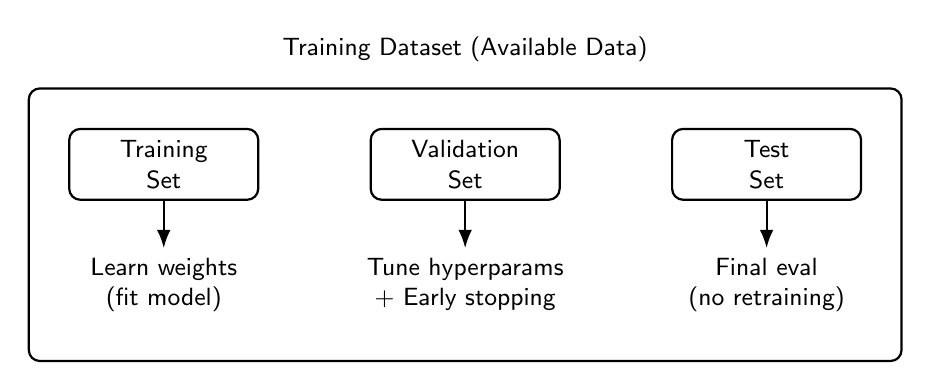
\begin{tikzpicture}[
        font=\sffamily\small,
        >=Latex,
        node distance=10mm,
        box/.style={draw, rounded corners, thick, align=center, minimum width=24mm, minimum height=9mm},
        lab/.style={align=center}
    ]
        % Top row
        \node[box] (train) {Training\\Set};
        \node[box, right=14mm of train] (val) {Validation\\Set};
        \node[box, right=14mm of val] (test) {Test\\Set};

        % Labels below + arrows
        \node[lab, below=6mm of train] (ltrain) {Learn weights\\(fit model)};
        \node[lab, below=6mm of val] (lval) {Tune hyperparams\\+ Early stopping};
        \node[lab, below=6mm of test] (ltest) {Final eval\\(no retraining)};

        \draw[->, thick] (train.south) -- (ltrain.north);
        \draw[->, thick] (val.south)   -- (lval.north);
        \draw[->, thick] (test.south)  -- (ltest.north);

        % Outer container with title
        \node[
            draw, rounded corners, thick, inner sep=5mm,
            fit=(train)(val)(test)(ltrain)(lval)(ltest),
            label={[yshift=2mm]above:Training Dataset (Available Data)}
        ] (container) {};
    \end{tikzpicture}
    \caption{Visualization of the relationships between training, validation, and test sets within the overall training dataset.}
    \label{fig:terminology-clarifications-dataset-split}
\end{figure}
    \subsection{Cross-Validation Techniques}

\definition{Cross-Validation} is the use of the \textbf{training dataset} to both: train the model (\emph{parameter fitting} and \emph{model selection}), and \textbf{estimate its error on new data}. In other words, we don't need a separate external test dataset for every trial, we can reuse the available data intelligently (e.g., part for training, part for checking generalization).

\highspace
\textcolor{Green3}{\faIcon[regular]{lightbulb} \textbf{Main Idea.}} Instead of holding out a single fixed portion (like in the simple \emph{hold-out} method), cross-validation systematically \textbf{rotates} which samples are used for training and which for validation. Each sample eventually acts as validation data once and training data many times. Thus, we can:
\begin{itemize}
    \item \textbf{Train multiple models} on different training subsets;
    \item \textbf{Validate} each on the complementary subset;
    \item \textbf{Average the validation errors} to get a more robust estimate of the model's true performance on unseen data.
\end{itemize}
It is especially useful when the dataset is limited, as it maximizes the use of available data for both training and validation. However, other techniques (like hold-out, LOOCV, K-Fold) are specific implementations of cross-validation with different trade-offs in terms of bias, variance, and computational cost. In the following, we explore some of these techniques.

\newpage

\subsubsection{Hold-Out Validation}\label{sec:hold-out-validation}

The \definition{Hold-Out Validation} (or \definition{Hold-Out Method}) is the simplest form of cross-validation. It consists of dividing the available dataset into \textbf{two or three subsets}, each serving a specific role in training, tuning, and evaluating the model. This method provides a first, practical way to test the \textbf{inductive hypothesis}, that a model performing well on unseen data will also generalize to future examples (page \pageref{def:inductive-hypothesis}).

\highspace
\begin{flushleft}
    \textcolor{Green3}{\faIcon{question-circle} \textbf{How does it work?}}
\end{flushleft}
In the typical \textbf{three-way split}, we start from the \textbf{training dataset}, i.e., all the data we can use to develop the model, we then split it into disjoint subsets:
\begin{itemize}
    \item \textbf{Training Set}: This subset is used to \textbf{parameter fitting}, i.e., to train the model by adjusting its weights based on the input-output pairs.
    \item \textbf{Validation Set}: This subset is used to \textbf{model selection}, i.e., to evaluate different model configurations (e.g., architectures, hyperparameters) and select the best one based on its performance on this set.
    \item \textbf{Test Set} (hold-out): This subset is used to \textbf{model assessment}, i.e., to provide an unbiased evaluation of the final model's performance on unseen data after training and validation are complete.
\end{itemize}
The steps are as follows:
\begin{enumerate}
    \item \important{Divide} the available dataset into training and validation (and possibly test) sets.
    \item \important{Train} the neural networks using only the training set.
    \item \important{Validate} periodically on the validation set to monitor generalization:
    \begin{itemize}
        \item Tune hyperparameters (e.g., learning rate, architecture) based on validation performance.
        \item Apply \emph{early stopping} if validation error starts to increase (indicating overfitting).
    \end{itemize}
    \item \important{Assess} the final model on the hold-out test set (data not seen during training) to estimate its true generalization error.
\end{enumerate}
The hold-out validation gives an estimate of how well the model performs on \emph{unseen data} by simulating future inputs using the reserved portion of the dataset. It's essentially a ``\textbf{miniature deployment test}'' performed before real-world use.

\newpage

\begin{flushleft}
    \textcolor{Red2}{\faIcon{exclamation-triangle} \textbf{Risks and Limitations}}
\end{flushleft}
While hold-out validation is straightforward and easy to implement, it has some limitations. The main risk is that \textbf{hold-out validation can be biased} depending on how the data are split:
\begin{enumerate}
    \item \important{Non-representative sampling}
    \begin{itemize}
        \item The validation set may not accurately reflect the data distribution.
        \item The estimated generalization error may be too optimistic or too pessimistic.
    \end{itemize}

    \item \important{Small datasets}
    \begin{itemize}
        \item If we hold out too many samples, there are too few left for training.
        \item If we hold out too few, the validation estimate becomes noisy and unreliable.
    \end{itemize}

    \item \important{Unbalanced classes (classification case)}
    \begin{itemize}
        \item If the classes are not represented equally in the training and validation sets, the model may not learn to generalize well across all classes.
        \item[\textcolor{Green3}{\faIcon{check}}] \textcolor{Green3}{\textbf{Solution:}} use \textbf{stratified sampling} (page \pageref{def:stratified-sampling}) to maintain class proportions in each subset.
    \end{itemize}

    \item \important{Single split variability}
    \begin{itemize}
        \item A different random split can yield a different result.
        \item The error estimate depends too much on ``which data'' ended up in the validation set.
        \item[\textcolor{Green3}{\faIcon{check}}] \textcolor{Green3}{\textbf{Solution:}}  Later, we will see more robust techniques (like \textbf{K-Fold Cross-Validation}) that mitigate this issue by averaging results over multiple splits.
    \end{itemize}
\end{enumerate}

\highspace
\begin{flushleft}
    \textcolor{Green3}{\faIcon{question-circle} \textbf{When to use Hold-Out Validation?}}
\end{flushleft}
Hold-out validation is most appropriate when:
\begin{itemize}
    \item[\textcolor{Green3}{\faIcon{check}}] When the \textbf{dataset is large enough} to afford separate training, validation and test sets without sacrificing training data. With large enough we mean at least a few thousand samples.
    \item[\textcolor{Green3}{\faIcon{check}}] When we want \textbf{fast model evaluation} without the computational overhead of more complex cross-validation methods (only one training phase).
    \item[\textcolor{Green3}{\faIcon{check}}] When small fluctuations in the validation split are not expected to significantly affect the model selection process.
\end{itemize}
    \subsubsection{Leave-One-Out Cross-Validation (LOOCV)}

\definition{Leave-One-Out Cross-Validation (LOOCV)} is a special case of \emph{K-Fold Cross-Validation} (next section) where the number of folds $K$ is equal to the number of samples $N$ in the dataset. It means that each data point acts \textbf{once} as validation data, and $N-1$ times as part of the training set.

\highspace
\begin{flushleft}
    \textcolor{Green3}{\faIcon{tools} \textbf{How does it work?}}
\end{flushleft}
\begin{enumerate}
    \item Given a dataset with $N$ samples:
    \begin{equation*}
        \mathcal{D} = \left\{
            \left(x_1, t_1\right),
            \left(x_2, t_2\right),
            \ldots,
            \left(x_N, t_N\right)
        \right\}
    \end{equation*}
    \item For each sample $i = 1, 2, \ldots, N$:
    \begin{itemize}
        \item Train the model on all samples except the $i$-th one:
        \begin{equation*}
            \mathcal{D}_{\text{train}}^{(i)} = \mathcal{D} \setminus \left\{ \left(x_i, t_i\right) \right\}
        \end{equation*}
        \item Validate (test) the model on the $i$-th sample:
        \begin{equation*}
            \mathcal{D}_{\text{val}}^{(i)} = \left\{ \left(x_i, t_i\right) \right\}
        \end{equation*}
    \end{itemize}
    \item Collect all validation errors $E_{i}$ from each iteration, and compute the \textbf{average error}:
    \begin{equation*}
        \hat{E}_{\text{LOOCV}} = \dfrac{1}{N} \cdot \sum_{i=1}^{N} E_{i}
    \end{equation*}
    This average error $\hat{E}_{\text{LOOCV}}$ gives an \textbf{almost unbiased estimate} of the model's generalization error.
\end{enumerate}

\highspace
\begin{flushleft}
    \textcolor{Red2}{\faIcon{exclamation-triangle} \textbf{Risks and Limitations}}
\end{flushleft}
While LOOCV maximizes data usage for training and provides a nearly unbiased error estimate, it has some drawbacks:
\begin{enumerate}
    \item \important{Computational Cost}. We must train the model $N$ times (once for each sample), which can be \textbf{prohibitively expensive} for large datasets or deep neural networks.
    \item \important{High variance in models}. Each training set differs by only one sample, so the models can be \textbf{very similar}. This can lead to high variance in the validation errors, making the average error estimate less stable.
    \item \important{Not practical for deep learning}. Neural networks often require thousands of training iterations to converge, making LOOCV impractical for large-scale problems.
\end{enumerate}

\newpage

\begin{flushleft}
    \textcolor{Green3}{\faIcon{question-circle} \textbf{When to use LOOCV?}}
\end{flushleft}
LOOCV has an \textbf{unbiased estimate} (each data point serves as validation once, so every sample influences the estimate equally) and an \textbf{efficient use of data} (almost all samples are used for training in each iteration, ideal when data are scarce). Thanks to these properties, LOOCV is particularly useful when:
\begin{itemize}
    \item[\textcolor{Green3}{\faIcon{check}}] When $N$ is \textbf{small} (e.g., a few hundred samples or less).
    \item[\textcolor{Green3}{\faIcon{check}}] When we want an \textbf{almost unbiased} generalization error estimate.
    \item[\textcolor{Green3}{\faIcon{check}}] When computation time is \textbf{not a concern} (e.g., simple models).
\end{itemize}
LOOCV approximates the \emph{true expected error} $E_{\text{test}}$ and it's nearly unbiased because each sample plays both roles, training and validation, but it tends to have \textbf{high variance} because each training set is almost identical, leading to similar models. However, for modern deep learning, it's mostly of \textbf{theoretical interest}, a conceptual benchmark rather than a practical tool.
    \subsubsection{K-Fold Cross-Validation}

\definition{K-Fold Cross-Validation} divides the available dataset into $K$ equally (or nearly equally) sized subsets, called \emph{folds}. The model is trained and validated $K$ times, each time using a different fold as the \textbf{validation set}, and the remaining $K-1$ folds as the \textbf{training set}. After completing all $K$ rounds, the $K$ validation errors are \textbf{averaged} to estimate the model's overall generalization performance.

\highspace
\begin{flushleft}
    \textcolor{Green3}{\faIcon{tools} \textbf{How does it work?}}
\end{flushleft}
\begin{enumerate}
    \item Given a dataset with $N$ samples:
    \begin{equation*}
        \mathcal{D} = \left\{
            \left(x_1, t_1\right),
            \left(x_2, t_2\right),
            \ldots,
            \left(x_N, t_N\right)
        \right\}
    \end{equation*}
    \item Split the dataset $\mathcal{D}$ into $K$ \emph{folds} (disjoint subsets):
    \begin{equation*}
        \mathcal{D} = \mathcal{D}_1 \cup \mathcal{D}_2 \cup \ldots \cup \mathcal{D}_K
    \end{equation*}
    Where each fold $\mathcal{D}_k$ contains approximately $\dfrac{N}{K}$ samples:
    \begin{equation*}
        \left| \mathcal{D}_k \right| \approx \dfrac{N}{K}, \quad \text{for } k = 1, 2, \ldots, K
    \end{equation*}
    \item For each fold $k = 1, 2, \ldots, K$:
    \begin{itemize}
        \item Train the model on the other $K-1$ folds (i.e., all folds except the $k$-th one, mathematically $\mathcal{D} \setminus \mathcal{D}_k$):
        \begin{equation*}
            \mathcal{D}_{\text{train}}^{(k)} = \bigcup_{\substack{j=1 \\ j \neq k}}^{K} \mathcal{D}_j
        \end{equation*}
        \item Validate (test) the model on the $k$-th fold:
        \begin{equation*}
            \mathcal{D}_{\text{val}}^{(k)} = \mathcal{D}_k
        \end{equation*}
        \item Compute the validation error $\hat{e}_{k}$ on the validation set $\mathcal{D}_{\text{val}}^{(k)}$.
    \end{itemize}
    \item Collect all validation errors $E_{k}$ from each iteration, and compute the \textbf{average error}:
    \begin{equation*}
        \hat{E}_{\text{K-Fold}} = \dfrac{1}{K} \cdot \sum_{k=1}^{K} \hat{e}_{k}
    \end{equation*}
    This average error $\hat{E}_{\text{K-Fold}}$ provides an estimate of the model's generalization error.
\end{enumerate}
Differently from LOOCV, K-Fold Cross-Validation allows us to choose a smaller $K$:
\begin{itemize}
    \item \important{5-Fold Cross-Validation} is the most commonly used value, balancing bias and variance in the error estimate.
    \item \important{10-Fold Cross-Validation} is also popular, especially in scenarios where more data is available, providing a slightly lower bias at the cost of increased computational time.
    \item \important{Stratified K($K = N$)-Fold Cross-Validation} equivalent to LOOCV, where each fold contains exactly one sample. Unbiased but computationally expensive.
    \item \important{2 or 3-Fold Cross-Validation} can be used for very large datasets where computational efficiency is a concern, but may lead to higher variance in the error estimate.
\end{itemize}

\highspace
\begin{flushleft}
    \textcolor{Red2}{\faIcon{exclamation-triangle} \textbf{Limitations}} \textbf{and} \textcolor{Green3}{\faIcon{check-circle} \textbf{Advantages}}
\end{flushleft}
\textbf{Compared to Hold-Out}, it uses the entire dataset more efficiently because each sample is used for validation once and for training $K-1$ times (lower bias). Also, \textbf{compared to LOOCV}, it is much cheaper computationally (only $K$ trainings instead of $N$).
\begin{itemize}
    \item[\textcolor{Green3}{\faIcon{check}}] \textcolor{Green3}{\textbf{Efficient data usage}}: all samples contribute to both training and validation.
    \item[\textcolor{Green3}{\faIcon{check}}] \textcolor{Green3}{\textbf{Reduced bias}}: the averaged approximates the expected generalization error better than a single split.
    \item[\textcolor{Green3}{\faIcon{check}}] \textcolor{Green3}{\textbf{Stability}}: more reliable than hold-out because the specific data division matter less.
    \item[\textcolor{Red2}{\faIcon{times}}] \textcolor{Red2}{\textbf{Computational cost}}: the model is trained $K$ times, still heavier than a single hold-out validation. For deep neural networks, this can be impractical.
    \item[\textcolor{Red2}{\faIcon{times}}] \textcolor{Red2}{\textbf{Data leakage risk}}: all processing (normalization, scaling, etc.) must be \textbf{recomputed inside each fold}, otherwise information from the validation folds can leak into the training folds.
    \item[\textcolor{Red2}{\faIcon{times}}] \textcolor{Red2}{\textbf{Variance in small datasets}}: if $K$ is too small, each fold may not represent the full data distribution well. 
\end{itemize}
    \subsubsection{Nested Cross-Validation}

When we train a neural network (or any machine learning model), we actually perform \textbf{two separate activities}:
\begin{itemize}
    \item \textbf{Model selection}: choose the \emph{best configuration} (e.g., hyperparameters, architecture) based on performance on a validation set.
    \item \textbf{Model assessment}: estimate the \emph{true generalization ability} of the final chosen model on unseen data.
\end{itemize}
\textcolor{Red2}{\faIcon{exclamation-triangle}} But here lies a \textbf{problem}: in most cross-validation setups, \textbf{we reuse the same data for both tasks}. That means we \textbf{peek} at our test data while tuning our model, leading to \textbf{optimistic bias} in our performance estimates.

\highspace
\textcolor{Red2}{\faIcon{question-circle} \textbf{Why that's a problem (hidden optimism)?}} Let's say we're testing 10 different neuronal network architectures and we run \textbf{5-fold cross-validation} ($K=5$) to see which performs best.
\begin{enumerate}
    \item We choose the one with the lowest average validation error across the 5 folds.
    \item Then we report that same average validation error as ``the model's performance''.
\end{enumerate}
\textcolor{Red2}{\faIcon{exclamation-triangle}} But this is \textbf{optimistically biased}, because:
\begin{itemize}
    \item We \textbf{used} the validation data to pick the best model.
    \item Therefore, the validation score no longer represents unseen data, because the model (and our choice) are \textbf{tuned} to those particular folds we used (even if indirectly).
\end{itemize}
So we get a number that looks great, but it's \textbf{too optimistic}, it doesn't reflect how the model would perform on truly unseen data.

\highspace
\begin{flushleft}
    \textcolor{Green3}{\faIcon{check-circle} \textbf{There is no more optimism with Nested Cross-Validation}}
\end{flushleft}
\definition{Nested Cross-Validation} is a technique that \textbf{separates model selection from model assessment} by introducing \textbf{two layers of cross-validation loops}:
\begin{itemize}
    \item An \textbf{outer loop} for \textbf{model assessment} (unseen test data). It evaluates \emph{how good that chosen configuration} really is on truly unseen data.
    \item An \textbf{inner loop} for \textbf{model selection} (tuning hyperparameters). It decides \emph{which configuration} performs best (uses only training data of that outer fold).
\end{itemize}
So now, when we report the average outer test error, it reflects \textbf{real generalization}, not the performance on data we optimized for.

\begin{examplebox}[: Nested Cross-Validation Analogy]
    Think of it like preparing for an exam:
    \begin{itemize}
        \item We take \textbf{practice tests} to decide the best study method (this is the \textbf{inner loop, model selection}).
        \item Then, we take the \textbf{final exam} to measure how well our preparation really worked (this is the \textbf{outer loop, model assessment}).
    \end{itemize}
    If we report our \emph{practice test} scores as our \emph{final exam} result, we'll be unrealistically confident, exactly what happens without nested cross-validation.
\end{examplebox}

\highspace
\begin{flushleft}
    \textcolor{Green3}{\faIcon{tools} \textbf{How does Nested Cross-Validation work?}}
\end{flushleft}
\begin{enumerate}
    \item \important{Outer Loop (Model Assessment)}:
    \begin{itemize}
        \item Split the entire dataset into $K$ \textbf{outer folds}:
        \begin{equation*}
            \mathcal{D} = \left\{ \mathcal{D}_1, \mathcal{D}_2, \ldots, \mathcal{D}_K \right\}
        \end{equation*}
        \item For each outer fold $k$:
        \begin{itemize}
            \item Reserve fold $\mathcal{D}_k^{\text{outer}}$ for \textbf{testing}.
            \item Use the remaining $K-1$ folds as the \textbf{training set} for model selection in the inner loop:
            \begin{equation*}
                \mathcal{D}_{\text{train}}^{\text{outer}} = \bigcup_{\substack{j=1 \\ j \neq k}}^{K} \mathcal{D}_j
            \end{equation*}
        \end{itemize}
    \end{itemize}
    \item \important{Inner Loop (Model Selection)}:
    \begin{itemize}
        \item Inside that outer training data $\mathcal{D}_{\text{train}}^{\text{outer}}$, perform another $K$-fold cross-validation, called \textbf{$M$-fold cross-validation}:
        \begin{equation*}
            \mathcal{D}_{\text{train}}^{\text{outer}} = \left\{ \mathcal{D}_1^{\text{inner}}, \mathcal{D}_2^{\text{inner}}, \ldots, \mathcal{D}_M^{\text{inner}} \right\}
        \end{equation*}
        To \textbf{tune hyperparameters} (e.g., learning rate, number of layers, etc.). The letter $M$ is used to distinguish it from the outer loop's $K$.
        \item Select the \hl{configuration} $\theta^{*}_{k}$ that gives the \textbf{lowest inner validation error averaged} over the $M$ inner folds:
        \begin{equation*}
            \theta^{*}_{k} = \arg\min_{\theta} \left(
                \dfrac{1}{M} \cdot \sum_{m=1}^{M} \text{Error}\left( \mathcal{D}_m^{\text{inner, val}}; \theta \right)
            \right)
        \end{equation*}
    \end{itemize}
    \item \important{Model Evaluation}:
    \begin{itemize}
        \item Retrain the model on \textbf{all inner folds combined} using the selected configuration $\theta^{*}_{k}$:
        \begin{equation*}
            \mathcal{D}_{\text{train}}^{\text{inner}} = \bigcup_{m=1}^{M} \mathcal{D}_m^{\text{inner}}
        \end{equation*}
        \item Evaluate it on the \textbf{outer test fold} $\mathcal{D}_k^{\text{outer}}$ to get the test error for that outer fold:
        \begin{equation*}
            \text{Test Error}_k = \text{Error}\left( \mathcal{D}_k^{\text{outer}}; \theta^{*}_{k} \right)
        \end{equation*}
        And \hl{store} the test error for that outer fold:
        \begin{equation*}
            e_k = \text{Test Error}_k
        \end{equation*}
    \end{itemize}
    \item \important{Average over outer folds}. After completing all $K$ outer folds, compute the overall performance estimate:
    \begin{equation*}
        \text{Overall Test Error} = \hat{E}_{\text{nested}} = \frac{1}{K} \sum_{k=1}^{K} e_k
    \end{equation*}
    This gives an \textbf{unbiased estimate} of the model's generalization performance.
\end{enumerate}

\highspace
\begin{flushleft}
    \textcolor{Red2}{\faIcon{exclamation-triangle} \textbf{Limitations}} \textbf{and} \textcolor{Green3}{\faIcon{check-circle} \textbf{Advantages}}
\end{flushleft}
\begin{itemize}
    \item[\textcolor{Green3}{\faIcon{check}}] Provides an \textbf{unbiased generalization estimate}, even after hyperparameter tuning.
    \item[\textcolor{Green3}{\faIcon{check}}] Ensures a clear \textbf{separation between selection and assessment}.
    \item[\textcolor{Green3}{\faIcon{check}}] Uses \textbf{all data efficiently} across different folds.
    \item[\textcolor{Red2}{\faIcon{times}}] \textbf{Computationally expensive}: Each outer folds contains a full inner cross-validation loop, so the model is trained $K \times M$ times. For deep neural networks, this can be prohibitive.
    \item[\textcolor{Red2}{\faIcon{times}}] \textbf{Complex implementation}: Careful bookkeeping is required to manage data splits and model configurations across nested loops. In other words, it's easy to make mistakes if not implemented carefully.
\end{itemize}
Some typical choices are $K=5$ for the outer loop and $M=3$ for the inner loop, balancing computational cost and reliable estimates. For more accurate estimates, $K=10$ and $M=5$ can be used, but at a higher computational cost. For small datasets, nested cross-validation is particularly beneficial to avoid overfitting during model selection, and a common choice is $K=10$ and $M=5$.

    \subsection{Preventing Overfitting}\label{sec:nn-preventing-overfitting}

So far we've seen:
\begin{itemize}
    \item \textbf{Overfitting}: when the model fits both the signal \emph{and} the noise in the training data, leading to poor generalization on unseen data.
    \item \textbf{Underfitting}: when the model is too simple to capture the underlying patterns in the data, resulting in poor performance on both training and test sets.
    \item \textbf{Cross-Validation}: how to detect when a model generalizes poorly using techniques like Hold-Out Validation, Leave-One-Out Cross-Validation (LOOCV), K-Fold Cross-Validation, and Nested Cross-Validation.
\end{itemize}
But detecting overfitting is only half the battle. The next crucial step is to implement strategies to \textbf{prevent or limit overfitting during training} and enhance the model's ability to generalize well to new, unseen data. This section presents the \textbf{three main families of solutions} that modern deep learning uses to \emph{control complexity} and \emph{improve generalization}.

\highspace
\textcolor{Red2}{\faIcon{exclamation-triangle} \textbf{The Core Problem:}} Neural networks have enormous representational power, by the \emph{Universal Approximation Theorem} (page \pageref{thm:universal-approximation-theorem}), they can approximate any continuous function. However, if they have \textbf{too many parameters}, and \textbf{too little data} (or data with noise), they will \textbf{memorize} rather than \textbf{learn}. Preventing overfitting is thus about \textbf{introducing constraints or checks} that force the model to extract \textbf{essential structure} from the data, not incidental details.

\highspace
\textcolor{Green3}{\faIcon{check-circle} \textbf{Overview of Prevention Techniques.}} In this section, we will explore three main strategies to prevent overfitting in neural networks:
\begin{enumerate}
    \item \textbf{Training control}: \important{Early Stopping technique} (\autopageref{sec:early-stopping}). This method stops training when validation error starts increasing.
    \item \textbf{Model complexity control}: \important{Regularization (Weight Decay, L2) technique} (\autopageref{sec:weight-decay-l2-regularization}). This method adds a penalty when weights grow too large, because large weights often indicate memorization.
    \item \textbf{Randomization / Model averaging}: \important{Dropout technique} (\autopageref{sec:nn-dropout-stochastic-regularization}). This method randomly deactivates neurons during training, forcing the network to learn redundant representations that generalize better.
\end{enumerate}
Each of these reduce the \textbf{effective capacity} of the network in a different way. Either by limiting how long it trains, how larger weights can grow, or how tightly neurons depend on each other.

\newpage

\begin{flushleft}
    \textcolor{Green3}{\faIcon{question-circle} \textbf{How these techniques relate to the Training Curve}}
\end{flushleft}
Similar to the curve of \textbf{Model Complexity vs. Error} shown in Figure \ref{fig:error-vs-model-complexity}, these techniques aim to find the optimal point where the model is complex enough to capture the underlying patterns in the data, but not so complex that it overfits. The \definition{Training vs. Validation Error Curve} plot (shown in Figure \ref{fig:training-validation-error-curve}) illustrates how training and validation errors evolve during training. The goal of these techniques is to keep the model in the region where both training and validation errors are low, avoiding the point where validation error starts to increase due to overfitting.

\begin{figure}[!htp]
    \centering
    \includegraphics[width=\textwidth]{img/neural-networks-and-overfitting/training-vs-validation-loss.pdf}
    \caption{This plot illustrates the \definition{Training vs. Validation Error Curve} during the training of a neural network. Initially, both training and validation errors decrease as the model learns from the data. However, after a certain point (epoch 57), the validation error starts to increase while the training error continues to decrease, indicating that the model is beginning to overfit the training data. The optimal stopping point is where the validation error is minimized, which can be achieved using techniques like Early Stopping.}
    \label{fig:training-validation-error-curve}
\end{figure}

\noindent
Furthermore, all \textbf{these techniques operationalize the Ockham's Razor principle} we saw earlier: \hl{``prefer the simplest model that explains the data well''} (page \hqpageref{sec:ockhams-razor}). By constraining the model's capacity in various ways, we encourage it to focus on the most salient features of the data, leading to better generalization and performance on unseen data.
    \subsubsection{Early Stopping}

During training, the \textbf{training error} keeps decreasing as the model learns to fit the training data better and better. However, at some point, the \textbf{validation error} starts to increase again, indicating that the model is beginning to overfit the training data (as we saw in \autoref{fig:training-validation-error-curve} on \autopageref{fig:training-validation-error-curve}). That's the signature of \textbf{overfitting}: the model is still improving on the training data, but getting worse on unseen data.

\highspace
The first and simplest method to prevent overfitting is \textbf{early stopping}. The idea is very straightforward: we stop the training process \textbf{right before} the validation error starts to rise.

\highspace
\begin{flushleft}
    \textcolor{Green3}{\faIcon{chart-line} \textbf{Monitoring Validation Error}}
\end{flushleft}
To apply early stopping, we need to monitor both:
\begin{itemize}
    \item The \textbf{training error/loss} $E_{\text{train}}(k)$ (measures how well the network fits the training data).
    \item The \textbf{validation error/loss} $E_{\text{val}}(k)$ (measures how well it generalizes to unseen data).
\end{itemize}
Where $k$ is the current training iteration (or epoch). So, during training, at each iteration (epoch) $k$, we look for the \textbf{epoch} $\boldsymbol{k}_{\boldsymbol{ES}}$ (Early Stopping iteration) that minimizes the validation error:
\begin{equation*}
    E_{\text{val}}(k) \text{ is minimal} \implies k = k_{ES}
\end{equation*}
Once we find $k_{ES}$, we stop training and use the model parameters (weights and biases) from that iteration for our final model.

\highspace
\begin{flushleft}
    \textcolor{Green3}{\faIcon{book} \textbf{Stopping Criteria (iteration $k_{ES}$)}}
\end{flushleft}
\begin{definitionbox}[: Early Stopping]
    \definition{Early Stopping} is a regularization technique that prevents overfitting by \textbf{monitoring the validation error during training} and \textbf{halting the learning process when the error begins to increase}.

    \highspace
    The stopping iteration $k_{ES}$ is defined as the epoch where the validation error $E_{\text{val}}(k)$ is minimized. Formally:
    \begin{equation}
        k_{ES} = \underset{k}{\text{argmin}} \; E_{\text{val}}(k)
    \end{equation}
    It marks the point of \textbf{best generalization}; beyond it, the network starts fitting noise rather than signal.

    \highspace
    By interrupting training at $k_{ES}$, the model parameters remain close to their optimal generalizing values, providing an \textbf{online estimate of the true generalization error}. With ``\emph{online estimate}'', we mean that we can assess the model's performance on unseen data without needing a separate test set at this stage; ``\emph{online}'' refers to the fact that this evaluation happens during the training process itself.
\end{definitionbox}

\highspace
However, simply stopping at the first sign of validation error increase can be problematic due to random fluctuations (noise) in the validation curve. So, in practice, we implement a more robust strategy. We usually use a \textbf{patience window} to avoid stopping too early due to random noise in the validation curve. The \definition{Patience Window} (or \definition{Patience Parameter}) defines \textbf{how many epochs} the training process should \textbf{wait after the last improvement in validation error} before deciding to stop. In other words, we don't stop immediately when $E_{\text{val}}(k)$ increases once; instead, we wait for a few epochs to see if it improves again (since small fluctuations can occur due to noise).

\highspace
\begin{examplebox}[: Early Stopping with Patience Window]
    Imagine this simplified validation loss curve during training (table values):
    \begin{center}
        \begin{tabular}{@{} c c c @{}}
            \toprule
            \textbf{Epoch} & \textbf{Validation Loss} & \textbf{Improvement?} \\
            \midrule
            $\dots$ & $\dots$ & $\dots$ \\
            10  & 0.40  & \textcolor{Green3}{\faIcon{check}} improvement \\[.3em]
            11  & 0.38  & \textcolor{Green3}{\faIcon{check}} improvement \\[.3em]
            12  & 0.37  & \textcolor{Green3}{\faIcon{check}} improvement \\[.3em]
            13  & 0.375 & \textcolor{Red2}{\faIcon{times}} slightly worse \\[.3em]
            14  & 0.373 & \textcolor{Green3}{\faIcon{check}} improvement \\[.3em]
            15  & 0.376 & \textcolor{Red2}{\faIcon{times}} worse again \\[.3em]
            16  & 0.379 & \textcolor{Red2}{\faIcon{times}} worse \\[.3em]
            17  & 0.382 & \textcolor{Red2}{\faIcon{times}} worse \\
            \bottomrule
        \end{tabular}
    \end{center}
    Suppose we set a \textbf{patience window of 2 epochs}, the algorithm will stop after \textbf{epoch 17}, because it waited for 2 epochs after the last improvement (epoch 14) and saw no new decrease in validation loss. If we had set a patience of 4 epochs, it would have waited until epoch 19 before stopping.
\end{examplebox}

\highspace
\textcolor{Red2}{\faIcon{exclamation-triangle} \textbf{Be careful: it's a heuristic!}} Early stopping with a \emph{patience window} is \textbf{not mathematically guaranteed} to find the optimal epoch $k_{ES}$; we might stop a few epochs \textbf{too early} or \textbf{too late}, depending on noise, random initialization, learning rate, and other hyperparameters. In formal terms, it doesn't \emph{guarantee} the true optimum, but it approximates a \textbf{local minimum in the generalization curve}, which is what we really want in practice. The local minimum corresponds to a model that generalizes well without overfitting, even if it's not the absolute best possible model.

\highspace
\begin{flushleft}
    \textcolor{Green3}{\faIcon{book} \textbf{Online Estimation of Generalization Error}}
\end{flushleft}
The Early Stopping method can be viewed as an \textbf{online estimation of the true generalization error}, because we continuously track the validation loss as the network learns, and the shape of that curve tells us when the model begins to overfit. So, we use validation data to \textbf{approximate the true test error dynamically} without needing to retrain multiple times. Thus, early stopping is like a \textbf{built-in regularizer}: it doesn't change the loss function, but limits training to the ``sweet spot'' where generalization is maximal. Where ``online'' means that this estimation happens during the training process itself, rather than after training is complete.

\highspace
\begin{flushleft}
    \textcolor{Red2}{\faIcon{exclamation-triangle} \textbf{Limitations}} \textbf{and} \textcolor{Green3}{\faIcon{check-circle} \textbf{Advantages}}
\end{flushleft}
\begin{itemize}
    \item[\textcolor{Green3}{\faIcon{check}}] \textbf{Simple \& efficient}: no modification to loss or architecture
    \item[\textcolor{Green3}{\faIcon{check}}] \textbf{Automatic}: modern frameworks can monitor and stop automatically.
    \item[\textcolor{Green3}{\faIcon{check}}] \textbf{Improves generalization} without additional parameters.
    \item[\textcolor{Red2}{\faIcon{times}}] Requires a \textbf{validation set}, which reduces training data slightly.
    \item[\textcolor{Red2}{\faIcon{times}}] Works best when validation loss is smooth (less noisy).
    \item[\textcolor{Red2}{\faIcon{times}}] The ``patience'' value and monitoring metric must be chosen carefully.
\end{itemize}
    \subsubsection{Hyperparameter Tuning}

After understanding \textbf{Early Stopping} (which stops training at the right moment), we now focus on \textbf{choosing the right model itself}; that is, deciding \emph{how big}, \emph{how deep}, \emph{how fast}, and \emph{how regularized} the network should be. This process is called \textbf{Hyperparameter Tuning}, and it's a \textbf{crucial step to control overfitting and improve generalization}.

\begin{definitionbox}[: Hyperparameter Tuning]
    \definition{Hyperparameter Tuning} is the process of \textbf{selecting the best model configuration}, that is, the combination of hyperparameters (such as the number of layers, neurons, learning rate, regularization, strength, etc.). That yields the \textbf{lowest validation error} and thus the best generalization ability.

    \highspace
    Unlike \textbf{parameters} (weights and biases), which are learned automatically during training, \textbf{hyperparameters} control \emph{how} learning occurs and \emph{how complex} the model can be.

    \highspace
    The optimal configuration:
    \begin{equation}
        \theta^{*} = \underset{\theta_{i}}{\arg\min} \; E_{\text{val}}\left(\theta_{i}\right)
    \end{equation}
    is chosen by \textbf{comparing validation errors} across candidate models, often within a cross-validation framework to reduce bias.
\end{definitionbox}

\begin{flushleft}
    \textcolor{Green3}{\faIcon{balance-scale} \textbf{Parameters vs. Hyperparameters}}
\end{flushleft}
The definition above highlights the distinction between \textbf{parameters} and \textbf{hyperparameters}:
\begin{itemize}
    \item \important{Parameters}: These are the internal \textbf{weights and biases} of the neural network that are \textbf{learned during training through optimization algorithms} like gradient descent. They directly influence the model's predictions, so they determine the function learned by the network.
    \item \important{Hyperparameters}: These are \textbf{external configurations set before training begins}. They include choices like the:
    \begin{itemize}
        \item \textbf{Number of layers}: This determines the depth of the network. More layers can capture more complex patterns but may also lead to overfitting.
        \item \textbf{Number of neurons per layer}: This controls the width of the network. More neurons can model more complex functions but increase the risk of overfitting.
        \item \textbf{Learning rate}: This is a crucial hyperparameter that controls how much to change the model in response to the estimated error each time the model weights are updated.
        \item \textbf{Batch size}: This defines the number of training examples utilized in one iteration. Smaller batch sizes can provide a more accurate estimate of the gradient but take longer to train. We have seen this in the \textbf{Stochastic Gradient Descent} (\emph{batch gradient descent}, \autoref{warn:perceptron-batch}, \autopageref{warn:perceptron-batch})
        \item \textbf{Regularization strength $\gamma$}: This controls the amount of regularization applied to the model to prevent overfitting. Higher values impose a stronger penalty on large weights. We will see this in future sections.
        \item \textbf{Dropout rate}: This defines the fraction of neurons to drop during training to prevent overfitting. A higher dropout rate means more neurons are ignored during each training iteration. Also this will be covered in future sections.
    \end{itemize}
    Hyperparameters are set \textbf{manually} by the user or \textbf{automatically}\break through hyperparameter optimization techniques (e.g., grid search, random search, Bayesian optimization). They control \emph{how} the model learns and \emph{how complex} it can become, thus affecting its ability to generalize to unseen data.
\end{itemize}

\highspace
\begin{flushleft}
    \textcolor{Green3}{\faIcon{question-circle} \textbf{Why is Hyperparameter tuning important? And why does it matter for overfitting?}}
\end{flushleft}
Hyperparameter tuning is essential for several reasons, especially in the context of overfitting. It determines the \textbf{model's capacity to learn from data} and its ability to generalize to unseen examples.

\begin{table}[!htp]
    \centering
    \begin{tabular}{@{} p{9.7em} l l @{}}
        \toprule
        \textbf{Hyperparameter} & \textbf{Low Value} & \textbf{High Value} \\
        \midrule
        Number of layers/neurons & Underfitting (too simple) & Overfitting (too complex) \\[.3em]
        Learning rate & Slow convergence & Unstable or overfitting \\[.3em]
        Regularization strength $\gamma$ & Weak penalty, overfit & Too strong, underfit \\[.3em]
        Dropout rate & Too little regularization & Too much, underfit \\
        \bottomrule
    \end{tabular}
    \caption{Impact of Hyperparameter Values on Model Performance.}
    \label{tab:hyperparameter-impact}
\end{table}

\noindent
In geneal, \textbf{too low values} of hyperparameters can lead to \textbf{underfitting}, where the model is too simple to capture the underlying patterns in the data. Conversely, \textbf{too high values} can lead to \textbf{overfitting}, where the model learns the training data too well, including its noise and outliers, resulting in poor generalization to new data. So tuning them correctly is essential to reach the \textbf{sweet spot} of generalization.

\newpage

\begin{flushleft}
    \textcolor{Green3}{\faIcon{cogs} \textbf{Hyperparameter Tuning Algorithm}}
\end{flushleft}
The \definition{Hyperparameter Tuning Algorithm} is not a real algorithm per se, but rather a \textbf{conceptual framework} for selecting the best hyperparameters based on validation performance. The input are:
\begin{itemize}
    \item A \textbf{set $\Theta$ of possible hyperparameter configurations}:
    \begin{equation*}
        \Theta = \left\{\theta_1, \theta_2, \dots, \theta_M\right\}
    \end{equation*}
    Where each $\theta_i$ is a specific combination of hyperparameter values (e.g., number of layers, learning rate, regularization strength, etc.), and $M$ is the total number of configurations to evaluate.
    \item A \textbf{training dataset} $\mathcal{D}_{\text{train}}$ used to train the model for each hyperparameter configuration.
    \item A \textbf{validation dataset} $\mathcal{D}_{\text{val}}$ used to evaluate the model's performance for each configuration. Here we assume that our dataset is large enough to be split into training and validation sets. If not, cross-validation techniques can be employed to make the most of limited data (hold-out method \autopageref{sec:hold-out-validation}, k-fold \autopageref{sec:k-fold-cross-validation} or leave-one-out cross-validation \autopageref{sec:leave-one-out-cross-validation}, or nested cross-validation \autopageref{sec:nested-cross-validation}).
\end{itemize}
The procedure is as follows:
\begin{enumerate}
    \item \important{Define candidate configurations}. Choose which hyperparameter combinations to evaluate. Each configuration $\theta_i$ should specify values for all relevant hyperparameters. For example, number of layers, number of neurons per layer, learning rate, regularization strength, etc.
    \item \important{For each configuration $\theta_i \in \Theta$}:
    \begin{enumerate}
        \item \important{Train} a neural network using $\mathcal{D}_{\text{train}}$ with the hyperparameters specified by $\theta_i$. This involves initializing the model, performing forward and backward passes, and updating weights according to the chosen optimization algorithm (we will see this in future sections).
        \item \important{Evaluate} its performance on the \textbf{validation set} $\mathcal{D}_{\text{val}}$ to compute the validation error $E_{\text{val}}(\theta_i)$. This error metric could be mean squared error, cross-entropy loss, accuracy, etc., depending on the task. If using cross-validation, average the validation errors across all folds to get a robust estimate.
    \end{enumerate}
    \item \important{Compare validation errors}. Identify the configuration that gives the \textbf{lowest validation error}:
    \begin{equation*}
        \theta^{*} = \underset{\theta_{i} \in \Theta}{\arg\min} \; E_{\text{val}}\left(\theta_{i}\right)
    \end{equation*}
    \item \important{Select the best model}. Keep the model trained with the optimal hyperparameters $\theta^{*}$, or retrain it from scratch using the \textbf{union of training} and \textbf{validation data} with the chosen hyperparameters to maximize the data available for learning.
    \item \important{(optional) Final test}. Evaluate the chosen model on a \textbf{separate test set} $\mathcal{D}_{\text{test}}$ to estimate its generalization performance on unseen data.
\end{enumerate}
The output of this procedure is the \textbf{optimal hyperparameter configuration} $\theta^{*}$ that minimizes the validation error, along with the \textbf{trained model} that can be used for predictions on new data, and an \textbf{estimate of its generalization performance} (from validation or test set).

\highspace
\begin{flushleft}
    \textcolor{Green3}{\faIcon{question-circle} \textbf{How to choose candidate hyperparameter configurations?}}
\end{flushleft}
In practice, candidate hyperparameter configurations are not chosen manually because this would be too time-consuming and inefficient. Instead, we use \textbf{automatic search methods} to explore the hyperparameter space effectively.

\highspace
Once we define the set of hyperparameters we want to tune, the following methods \textbf{automatically explore} different configurations and identify which one minimizes the \textbf{validation error} (or maximizes validation accuracy, depending on the task). The three classical methods are:
\begin{enumerate}
    \item \definition{Grid Search} (\hl{Exhaustive Search on a Discrete Grid}). This method evaluates the model on \textbf{all possible combinations} of a predefined set of hyperparameter values. For example, we define a \textbf{grid} for each hyperparameter:
    \begin{equation*}
        \eta \in \left\{0.001, 0.01, 0.1\right\} \qquad
        \gamma \in \left\{0.01, 0.1, 1.0\right\} \qquad
        \text{layers} \in \left\{2, 3, 4\right\} \qquad
        \dots
    \end{equation*}
    Then the algorithm trains a model for \textbf{every combination} of these values:
    \begin{equation*}
        \Theta = \left\{\left(\eta, \gamma, \text{layers, \ldots}\right) \, \mid \, \eta \in \{\ldots\}, \,\gamma \in \{\ldots\}, \,\text{layers} \in \{\ldots\}, \, \ldots\right\}
    \end{equation*}
    After training and evaluating each configuration, the one with the lowest validation error is selected (minimum $E_{\text{val}}$).
    \begin{itemize}
        \item[\textcolor{Green3}{\faIcon{check}}] \textcolor{Green3}{\textbf{Advantages}}
        \begin{itemize}
            \item[\textcolor{Green3}{\faIcon{check}}] Simple and systematic.
            \item[\textcolor{Green3}{\faIcon{check}}] Parallelizable and easy to implement.
        \end{itemize}
        \item[\textcolor{Red3}{\faIcon{exclamation-triangle}}] \textcolor{Red2}{\textbf{Limitations}}
        \begin{itemize}
            \item[\textcolor{Red2}{\faIcon{times}}] Computationally expensive (combinations grow exponentially\break with more hyperparameters). Also, parallelizable only if enough resources are available.
            \item[\textcolor{Red2}{\faIcon{times}}] Many evaluations wasted on unimportant regions of the hyperparameter space.
            \item[\textcolor{Red2}{\faIcon{times}}] Works well only with a \emph{few} hyperparameters or \emph{coarse grids}.
        \end{itemize}
    \end{itemize}


    \item \definition{Random Search} (\hl{Stochastic Sampling of Hyperparameter Space}). Instead of evaluating all combinations, this method \textbf{randomly samples} hyperparameter configurations from specified distributions. For example, we define ranges or distributions for each hyperparameter:
    \begin{align*}
        \eta &\sim \text{Uniform}(0.001, 0.1) \\[.3em]
        \gamma &\sim \text{LogUniform}(0.01, 1.0) \\[.3em]
        \text{layers} &\sim \text{DiscreteUniform}\{2, 3, 4\} \\[.3em]
        & \ldots
    \end{align*}
    Then the algorithm samples $N$ configurations randomly:
    \begin{equation*}
        \Theta = \left\{\theta_1, \theta_2, \dots, \theta_N\right\}
    \end{equation*}
    After training and evaluating each sampled configuration, the one with the lowest validation error is selected. This method is \textbf{much more efficient than grid search}, because typically only a few hyperparameters significantly impact performance.
    \begin{itemize}
        \item[\textcolor{Green3}{\faIcon{check}}] \textcolor{Green3}{\textbf{Advantages}}
        \begin{itemize}
            \item[\textcolor{Green3}{\faIcon{check}}] Covers the search space more efficiently.
            \item[\textcolor{Green3}{\faIcon{check}}] Works better for high-dimensional spaces.
            \item[\textcolor{Green3}{\faIcon{check}}] Can easily add or extend hyperparameters.
        \end{itemize}
        \item[\textcolor{Red3}{\faIcon{exclamation-triangle}}] \textcolor{Red2}{\textbf{Limitations}}
        \begin{itemize}
            \item[\textcolor{Red2}{\faIcon{times}}] Still blind, don't use information from previous trials.
            \item[\textcolor{Red2}{\faIcon{times}}] May miss the best configuration by chance.
        \end{itemize}
    \end{itemize}


    \item \definition{Bayesian Optimization} (\hl{Probabilistic Model-Based Search}, \hl{Learning from Past Trials}). The idea is simple yet powerful. Model the function:
    \begin{equation*}
        f\left(\theta\right) = E_{\text{val}}\left(\theta\right)
    \end{equation*}
    As an \textbf{unknown function} (black box) and use \textbf{probabilistic reasoning} to decide which hyperparameters to test next. The steps are:
    \begin{enumerate}
        \item Use previous evaluations to build a \textbf{probabilistic surrogate model} (e.g. a Gaussiano Process, Tree Parzen Estimator, etc.) that approximates the relationship between hyperparameters and validation error ($f(\theta)$).
        \item Define an \textbf{acquisition function} (e.g. Expected Improvement, Upper Confidence Bound, etc.) that quantifies the potential benefit of evaluating a new configuration based on the surrogate model. It balances \textbf{exploration} (trying uncertain areas) and \textbf{exploitation} (focusing on promising areas).
        \item Choose the next configuration $\theta_{\text{next}}$ to evaluate by maximizing the acquisition function (i.e., the configuration that is expected to yield the most improvement).
        \item Now, train the model with $\theta_{\text{next}}$, evaluate its validation error\break $E_{\text{val}}(\theta_{\text{next}})$, and update the surrogate model with this new data point.
        \item Repeat steps 2-4 until a stopping criterion is met (e.g., a maximum number of evaluations or convergence).
    \end{enumerate}
    This method is not a naive search; it \textbf{learns from past evaluations} to make informed decisions about which hyperparameters to test next, leading to more efficient optimization.
    \begin{itemize}
        \item[\textcolor{Green3}{\faIcon{check}}] \textcolor{Green3}{\textbf{Advantages}}
        \begin{itemize}
            \item[\textcolor{Green3}{\faIcon{check}}] \textbf{Much fewer evaluations} needed for good performance.
            \item[\textcolor{Green3}{\faIcon{check}}] Adapts search intelligently (guided by prior results).
            \item[\textcolor{Green3}{\faIcon{check}}] Suitable for \textbf{expensive models} (deep networks, large datasets).
        \end{itemize}
        \item[\textcolor{Red3}{\faIcon{exclamation-triangle}}] \textcolor{Red2}{\textbf{Limitations}}
        \begin{itemize}
            \item[\textcolor{Red2}{\faIcon{times}}] Implementation complexity (requires probabilistic modeling).
            \item[\textcolor{Red2}{\faIcon{times}}] Needs a meaningful continuous search space (discrete hyperparameters can be tricky).
            \item[\textcolor{Red2}{\faIcon{times}}] Slower per iteration (but far fewer iterations needed).
        \end{itemize}
    \end{itemize}
\end{enumerate}
These methods follow the same underlying goal: \textbf{minimize the validation error} by efficiently exploring the hyperparameter space
\begin{equation*}
    \theta^{*} = \underset{\theta_{i} \in \Theta}{\arg\min} \; E_{\text{val}}\left(\theta_{i}\right)
\end{equation*}
But they differ in \textbf{\emph{how} they select candidate configurations} to evaluate, balancing exploration and exploitation in different ways.
    \subsubsection{Weight Decay (L2 Regularization)}

The \definition{Weight Decay} (or \definition{L2 Regularization}) is a widely used technique to prevent overfitting in neural networks by adding a penalty term to the loss function that discourages large weights. This method helps to keep the model simpler and more generalizable by constraining the magnitude of the weights.

\highspace
The key idea behind weight decay is to penalize overly large weights to prevent the network from overfitting training noise. When we train a neural network, we minimize a \textbf{loss function} (e.g. MSE regression or cross-entropy for classification):
\begin{equation*}
    E_{\text{train}}(w) = \frac{1}{N} \sum_{i=1}^{N} \mathcal{L}\left(y_i, f\left(x_i; w\right)\right)
\end{equation*}
If we let the optimization freely minimize this error, the network might use \textbf{very large weights} to fit every detail, creating a complex,oscillating decision surface that produces low training error but poor generalization to unseen data (i.e., \textbf{overfitting}). To counter this, we add a \textbf{penalty on the magnitude of weights} to the loss function:
\begin{equation*}
    E_{\text{reg}}(w) = E_{\text{train}}(w) + \frac{\gamma}{2} \sum_{q} w_q^2
\end{equation*}
Where:
\begin{itemize}
    \item $w_q$ is the $q$-th weight in the network.
    \item $\gamma > 0$ is the regularization parameter that controls the strength of the penalty (sometimes called \textbf{weight decay coefficient}). A larger $\gamma$ encourages smaller weights, leading to a simpler model (more bias, less variance), while a smaller $\gamma$ allows for more complex models (less bias, more variance).
\end{itemize}
This makes the optimization prefer \textbf{small, smooth weights}, producing\break smoother mappings from inputs to outputs, which helps in generalization.

\highspace
In other words, the optimizer now minimizes both \textbf{error} and \textbf{weight energy}. This discourages the model from relying too heavily on any single feature or neuron, promoting a more distributed representation that is less likely to overfit the training data (the network learns gentler transformations, \textbf{simpler hypotheses}).

\highspace
\begin{definitionbox}[: Weight Decay (L2 Regularization)]
    \definition{Weight Decay}, or \definition{L2 Regularization}, is a technique that prevents overfitting by adding a \textbf{penalty on the magnitude of the network's weights} to the loss function. The regularized loss function is:
    \begin{equation}
        E_{\text{reg}}(w) = E_{\text{train}}(w) + \frac{\gamma}{2} \sum_{q} w_q^2
    \end{equation}
    Where:
    \begin{itemize}
        \item $E_{\text{train}}(w)$ is the original training loss (e.g., MSE or cross-entropy).
        \item $w_q$ are the weights of the neural network.
        \item $\gamma > 0$ is the regularization parameter controlling the strength of the penalty.
    \end{itemize}
    By discouraging large weights, the model learns smoother mappings and achieves better generalization, effectively limiting its complexity.
\end{definitionbox}

\begin{flushleft}
    \textcolor{Green3}{\faIcon{balance-scale} \textbf{Relation to Early Stopping}}
\end{flushleft}
Early Stopping limited training time to prevent overfitting (\autopageref{sec:early-stopping}), while \textbf{weight decay directly limits the magnitude of parameters}. Both methods implement the Ockham's Razor principle by favoring simpler models that generalize better, but act at different stages:
\begin{itemize}
    \item \textbf{Early Stopping stops training} when validation error starts to rise, so before weights can grow too large.
    \item \textbf{Weight Decay continuously penalizes} large weights during training, keeping them small throughout the process.
\end{itemize}

\begin{figure}[!htp]
    \centering
    \includegraphics[width=\textwidth]{img/neural-networks-and-overfitting/weight-decay-plot.pdf}
    \caption{A simulation of polynomial regression with two different fits: one without regularization (large, oscillating weights, overfitting the data) and one with L2 regularization (smaller weights, smoother fit). The L2 regularized model generalizes better to unseen data.}
    \label{fig:weight-decay-l2-regularization}
\end{figure}

\newpage

\begin{flushleft}
    \textcolor{Green3}{\faIcon{book} \textbf{Bayesian Interpretation (MAP vs MLE)}}
\end{flushleft}
When we train a neural network, we're finding parameters $w$ that best explain the data $D = \left\{x_i, y_i\right\}$, where $x_i$ are inputs and $y_i$ are outputs. There are two main approaches to estimate these parameters:
\begin{itemize}
    \item \textbf{Maximum Likelihood Estimation (MLE)} (\autopageref{sec:maximum-likelihood-estimation}): choose the parameters $w$ that \textbf{maximize the probability of the data given the model}:
    \begin{equation*}
        w_{\text{MLE}} = \arg\max_{w} P\left(D \, \mid \, w\right)
    \end{equation*}
    Or equivalently, minimize the negative log-likelihood (which corresponds to minimizing the training error $E_{\text{train}}(w)$):
    \begin{equation*}
        w_{\text{MLE}} = \arg\min_{w} -\log P\left(D \, \mid \, w\right) \equiv \arg\min_{w} E_{\text{train}}(w)
    \end{equation*}
    That's just the \textbf{training loss} we usually minimize (like MSE or cross-entropy).
    \begin{itemize}
        \item[\textcolor{Green3}{\faIcon{check}}] MLE fits the data as best as possible.
        \item[\textcolor{Red2}{\faIcon{times}}] But it can lead to overfitting, especially with complex models and limited data. This is because MLE doesn't penalize complex parameters.
    \end{itemize}

    
    \item \textbf{Maximum A Posteriori Estimation (MAP)}: instead of trusting data blindly, we also include \textbf{prior beliefs} about what weights are likely. Let's explain this step by step. When we use \textbf{MLE}, we're saying: ``\emph{we don't know anything about the parameters $w$; just find the ones that make the data as likely as possible}''. That's pure \textbf{data fitting}. But what if we \emph{do} have priori knowledge? For example, we might believe that weights shouldn't be too large (to avoid overfitting), and most weights should be closer to zero (the network should be simple). Then we can express this belief \textbf{probabilistically}, by giving each possible value of $w$ a \textbf{prior probability} $P(w)$ that reflects \textbf{how plausible we think that value is before seeing any data}. Here, MAP combines this belief with the observed data.
    
    \highspace
    We want the \textbf{posterior probability} of the weights given the data:
    \begin{equation*}
        P\left(w \, \mid \, D\right) = \dfrac{P\left(D \, \mid \, w\right) P\left(w\right)}{P\left(D\right)}
    \end{equation*}
    \begin{itemize}
        \item $P\left(D \, \mid \, w\right)$ is the \textbf{likelihood} of the data given weights (same as in MLE).
        \item $P\left(w\right)$ is the \textbf{prior} probability of weights (our belief about weights before seeing data).
        \item $P\left(w \, \mid \, D\right)$ is the \textbf{posterior} probability of weights given the data (what we believe about weights after seeing data).
        \item $P\left(D\right)$ is the \text{evidence} (normalizing constant).
    \end{itemize}
    The \definition{Maximum A Posteriori (MAP)} estimation means: choose the weights $w$ that \textbf{maximize the posterior probability} $P\left(W \, \mid \, D\right)$:
    \begin{equation*}
        w_{\text{MAP}} = \arg\max_{w} P\left(w \, \mid \, D\right)
    \end{equation*}
    Using Bayes' rule, we can rewrite this as:
    \begin{equation*}
        w_{\text{MAP}} = \arg\max_{w} \dfrac{P\left(D \, \mid \, w\right) P\left(w\right)}{P\left(D\right)} = \arg\max_{w} P\left(D \, \mid \, w\right) P\left(w\right)
    \end{equation*}
    Since $P(D)$ is constant with respect to $w$, we can ignore it in the optimization. Taking logs, we get:
    \begin{equation*}
        w_{\text{MAP}} = \arg\max_{w} \left[ \log P\left(D \, \mid \, w\right) + \log P\left(w\right) \right]
    \end{equation*}
    Where the \textbf{first term} fits the data (like MLE), and the \textbf{second term} adds a \emph{regularization effect} (our prior belief about weights).
\end{itemize}
To \textbf{connect this to weight decay}, we need to choose a specific prior $P(w)$. A common choice is a \textbf{Gaussian prior} centered at zero:
\begin{equation*}
    P\left(w\right) = \prod_{q} \dfrac{1}{\sqrt{2 \pi \sigma^2}} \exp\left(-\dfrac{w_q^2}{2 \sigma^2}\right)
\end{equation*}
This prior says that we believe weights are likely to be small (close to zero), with variance $\sigma^2$ controlling how strongly we believe this. Taking the log of this prior gives:
\begin{equation*}
    \log P\left(w\right) = -\sum_{q} \dfrac{w_q^2}{2 \sigma^2} + \text{constant}
\end{equation*}
Ignoring constants, the MAP objective becomes:
\begin{equation*}
    w_{\text{MAP}} = \arg\max_{w} \left[ \log P\left(D \, \mid \, w\right) - \sum_{q} \dfrac{w_q^2}{2 \sigma^2} \right]
\end{equation*}
Or equivalently, minimizing the negative log-posterior:
\begin{equation*}
    w_{\text{MAP}} = \arg\min_{w} \left[ -\log P\left(D \, \mid \, w\right) + \sum_{q} \dfrac{w_q^2}{2 \sigma^2} \right]
\end{equation*}
This is exactly the same as minimizing the regularized loss function with weight decay:
\begin{equation*}
    E_{\text{reg}}(w) = E_{\text{train}}(w) + \frac{\gamma}{2} \sum_{q} w_q^2
\end{equation*}
Where $\gamma = \dfrac{1}{\sigma^2}$. Thus, \textbf{weight decay can be interpreted as MAP estimation with a Gaussian prior on weights}. This Bayesian perspective shows that weight decay not only helps prevent overfitting but also incorporates prior beliefs about model simplicity into the learning process.

\begin{figure}[!htp]
    \centering
    \includegraphics[width=\textwidth]{img/neural-networks-and-overfitting/weight-decay-l2-regularization.pdf}
    \caption{Bayesian interpretation of Weight Decay (L2 Regularization): MLE focuses solely on fitting the data, while MAP incorporates prior beliefs about weights, leading to more generalizable models. We have simulated a one-dimensional weight $w$: the \textbf{likelihood} $P\left(D \, \mid \, w\right)$ is peaked around some data-fitted value (like MLE); the \textbf{prior} $P(w)$ is a Gaussian centered at zero (we believe small weights are more likely); the \textbf{posterior} $P\left(w \, \mid \, D\right)$ combines (product) both, resulting in a peak that balances data fit and weight size.}
\end{figure}

\newpage

\begin{flushleft}
    \textcolor{Green3}{\faIcon{book} \textbf{Gaussian Priori Explanation}}
\end{flushleft}
\textcolor{Green3}{\faIcon{question-circle} \textbf{What is a prior over weights?}} When we train a model, we want to find good values for all weights $w_q$. If we follow a \textbf{Bayesian approach}, we say: each weight $w_q$ is a random variable, and before seeing data we have a belief about how likely different values are. This belief is encoded in a \textbf{prior distribution}.

\highspace
\textcolor{Green3}{\faIcon{question-circle} \textbf{Choosing a Gaussian Prior.}} A natural, simple choice for this prior is a \textbf{Gaussian (normal) distribution} centered at zero:
\begin{equation*}
    P\left(w_q\right) = \dfrac{1}{\sqrt{2 \pi \sigma^2}} \exp\left(-\dfrac{w_q^2}{2 \sigma^2}\right)
\end{equation*}
Intuitively:
\begin{itemize}
    \item The mean is zero, so small weights are more probable than large ones.
    \item The variance $\sigma^2$ controls how strongly we believe this:
    \begin{itemize}
        \item A small $\sigma^2$ means we strongly believe weights should be close to zero (less flexibility).
        \item A large $\sigma^2$ means we allow for larger weights (more flexibility).
    \end{itemize}
\end{itemize}
Assuming independence between weights, the joint prior over all weights is:
\begin{equation*}
    P\left(w\right) = \prod_{q} P\left(w_q\right) = \prod_{q} \dfrac{1}{\sqrt{2 \pi \sigma^2}} \exp\left(-\dfrac{w_q^2}{2 \sigma^2}\right)
\end{equation*}
So the prior over all weights is a multivariate Gaussian with diagonal covariance. Taking the log of this prior gives:
\begin{equation*}
    \log P\left(w\right) = \sum_{q} \log P\left(w_q\right) = -\dfrac{1}{2 \sigma^2} \sum_{q} w_q^2 + \text{constant}
\end{equation*}

\highspace
\textcolor{Green3}{\faIcon{question-circle} \textbf{Combine with likelihood (training error.)}} The MAP objective (as derived earlier) is:
\begin{equation*}
    w_{\text{MAP}} = \arg\max_{w} \left[ \log P\left(D \, \mid \, w\right) + \log P\left(w\right) \right]
\end{equation*}
Equivalently, minimizing the negative log-posterior:
\begin{equation*}
    E_{\text{reg}}(w) = -\log P\left(D \, \mid \, w\right) - \log P\left(w\right)
\end{equation*}
Replace $-\log P\left(D \, \mid \, w\right)$ with the \textbf{training loss} $E_{\text{train}}(w)$, and substitute the log prior:
\begin{equation*}
    E_{\text{reg}}(w) = E_{\text{train}}(w) + \dfrac{1}{2 \sigma^2} \sum_{q} w_q^2 + \text{constant}
\end{equation*}
Define $\gamma = \dfrac{1}{\sigma^2}$, we get:
\begin{equation*}
    E_{\text{reg}}(w) = E_{\text{train}}(w) + \dfrac{\gamma}{2} \sum_{q} w_q^2
\end{equation*}
This is exactly the weight decay regularization term! Thus, assuming a Gaussian prior on weights leads directly to L2 regularization in the MAP framework.

\begin{deepeningbox}[: What is a Multivariate Gaussian with Diagonal Covariance?]
    If we have a \textbf{single weight} $w_1$, we can describe our belief about it as a \textbf{univariate Gaussian}:
    \begin{equation*}
        P\left(w_1\right) = \dfrac{1}{\sqrt{2 \pi \sigma^2}} \exp\left(-\dfrac{\left(w_1 - 0\right)^2}{2 \sigma^2}\right)
    \end{equation*}
    That's just the classic bell curve centered at zero, spreading depending on $\sigma^2$.

    \highspace
    Now suppose we have \textbf{two weights} $w_1$ and $w_2$. We could model their joint belief as a \textbf{2D Gaussian distribution}:
    \begin{equation*}
        P\left(w_1, w_2\right) = \dfrac{1}{2 \pi \left|\Sigma\right|^{1/2}} \exp\left(-\dfrac{1}{2} \begin{bmatrix} w_1 \\ w_2 \end{bmatrix}^T \Sigma^{-1} \begin{bmatrix} w_1 \\ w_2 \end{bmatrix}\right)
    \end{equation*}
    Where $\Sigma$ is the \textbf{covariance matrix}. This tells us \textbf{how the two weights vary together}.

    \highspace
    The covariance matrix $\Sigma$ looks like this:
    \begin{equation*}
        \Sigma = \begin{bmatrix} \sigma_1^2 & \rho \sigma_1 \sigma_2 \\ \rho \sigma_1 \sigma_2 & \sigma_2^2 \end{bmatrix}
    \end{equation*}
    Where:
    \begin{itemize}
        \item $\sigma_1^2$ and $\sigma_2^2$ are the variances of $w_1$ and $w_2$.
        \item $\rho$ is the correlation coefficient between $w_1$ and $w_2$.
        \begin{itemize}
            \item If $\rho = 0$, the weights are \textbf{independent} (no correlation). This means changing $w_1$ doesn't affect $w_2$.
            \item If $\rho \neq 0$, the weights are \textbf{correlated} (changing one affects the other). This means if $w_1$ increases, $w_2$ might also tend to increase (if $\rho > 0$) or decrease (if $\rho < 0$).
        \end{itemize}
    \end{itemize}
    When we assume the weights are \textbf{independent}, we set $\rho = 0$. This simplifies the \textbf{covariance matrix to a diagonal matrix}, because the off-diagonal terms (which represent correlations) become zero:
    \begin{equation*}
        \Sigma = \begin{bmatrix} \sigma_1^2 & 0 & 0 & \dots \\ 0 & \sigma_2^2 & 0 & \vdots \\ 0 & 0 & \sigma_3^2 & \vdots \\ \vdots & \vdots & \vdots & \ddots \end{bmatrix}
    \end{equation*}
    Then the multivariate Gaussian \textbf{factorizes} into independent 1D Gaussians for each weight:
    \begin{equation*}
        P\left(w\right) = \prod_{q} \dfrac{1}{\sqrt{2 \pi \sigma_q^2}} \exp\left(-\dfrac{w_q^2}{2 \sigma_q^2}\right)
    \end{equation*}
    Each weight has its own Gaussian prior, and they don't influence each other. That's exactly what we assumed: each $w_q$ has its own $\mathcal{N}\left(0, \sigma^{2}\right)$ prior, and all weights are independent.

    \highspace
    Finally, when the covariance is diagonal ($\rho = 0$ and equal for all weights), we get:
    \begin{equation*}
        \Sigma = \sigma^2 I
    \end{equation*}
    Where $I$ is the identity matrix. This means that the log prior simplifies to:
    \begin{equation*}
        -\log P\left(w\right) = \dfrac{1}{2 \sigma^{2}} w^{T} w = \dfrac{1}{2 \sigma^{2}} \sum_{q} w_q^2
    \end{equation*}
    \hl{Which is exactly the L2 regularization term we use in weight decay!} So the assumption of a \emph{multivariate Gaussian with diagonal covariance} is what mathematically justifies the standard \textbf{weight decay formula}.
\end{deepeningbox}

\highspace
\begin{flushleft}
    \textcolor{Green3}{\faIcon{question-circle} \textbf{How do we choose the right regularization strength $\gamma$?}}
\end{flushleft}
Different values of $\gamma$ change how much we penalize large weights:
\begin{itemize}
    \item $\gamma = 0$ means no regularization (just MLE, prone to overfitting).
    \item $\gamma$ small means weak regularization (allows larger weights, more complex models).
    \item $\gamma$ large means strong regularization (forces weights to be small, simpler models).
\end{itemize}
So we must find the \textbf{optimal} $\gamma = \gamma^*$ that gives the \textbf{best generalization}. The idea is to split our data into:
\begin{itemize}
    \item A \textbf{training set} for fitting the weights $w$.
    \item A \textbf{validation set} for evaluating performance for each candidate $\gamma$.
\end{itemize}
Practically:
\begin{enumerate}
    \item Choose a range of candidate $\gamma$ values, for example:
    \begin{equation*}
        \left|
            10^{-5}, 10^{-4}, 10^{-3}, 10^{-2}, 10^{-1}, 1, 10
        \right|
    \end{equation*}
    \item For each candidate $\gamma$:
    \begin{itemize}
        \item Train the neural network with regularized loss:
        \begin{equation*}
            E_{\text{reg}}(w) = E_{\text{train}}(w) + \dfrac{\gamma}{2} \sum_{q} w_q^2
        \end{equation*}
        \item Compute validation error on the validation set:
        \begin{equation*}
            E_{\text{val}}(w) = E_{\text{val}}(w) + \dfrac{\gamma}{2} \sum_{q} w_q^2
        \end{equation*}
    \end{itemize}
    \item Pick the $\gamma^*$ that gives the lowest validation error:
    \begin{equation}
        \gamma^* = \arg\min_{\gamma} E_{\text{val}}
    \end{equation}
    \item Finally, retrain the network \textbf{on all data} using the selected $\gamma^*$ to get the final model.
\end{enumerate}
This cross-validation approach ensures we select a regularization strength that balances fitting the training data well while maintaining good generalization to unseen data.
    \subsubsection{Dropout (Stochastic Regularization)}\label{sec:nn-dropout-stochastic-regularization}

Even with weight decay and early stopping, large networks can still \textbf{overfit} because \textbf{neurons learn to co-adapt} too much. For example, neuron $A$ might learn to rely on neuron $B$ being active to make its predictions. If $B$ overfits, then $A$ will also overfit. We need a way to \textbf{force independence} among neurons, to make the network robust to missing or noisy signals.

\highspace
\textcolor{Green3}{\faIcon[regular]{lightbulb} \textbf{The Idea.}} During training, we \textbf{randomly ``drop'' neurons} (i.e., set their output to 0) with a certain probability $p$, independently at each training iteration.
\begin{itemize}
    \item Each forward pass uses a \textbf{different random subnetwork}.
    \item The model can't rely on any specific neuron always being present, so it must learn \textbf{redundant representations}.
\end{itemize}
\hl{Without dropout}, the activation of neuron $j$ in layer $l$ is:
\begin{equation*}
    h_j^{(l)} = g\left( \sum_{i} w_{ij}^{(l)} h_i^{(l-1)} + b_j^{(l)} \right)
\end{equation*}
\begin{itemize}
    \item $h_{i}^{(l-1)}$ are the activations from the previous layer.
    \item $w_{ij}^{(l)}$ are the weights connecting neuron $i$ in layer $l-1$ to neuron $j$ in layer $l$.
    \item $b_j^{(l)}$ is the bias term for neuron $j$ in layer $l$.
    \item $g(\cdot)$ is the activation function (e.g., tanh, sigmoid).
\end{itemize}
\definition{Dropout} introduces a random \textbf{mask} $m_j^{(l)}$ for each neuron, sampled from a \textbf{Bernoulli distribution} with parameter $p$ (the probability of \textbf{keeping} the neuron). Formally:
\begin{equation}
    m_j^{(l)} \sim \text{Bernoulli}(p) \Rightarrow m_j^{(l)} = \begin{cases}
        1 & \text{with probability } p \text{ neuron is kept} \\
        0 & \text{with probability } 1-p \text{ neuron is dropped}
    \end{cases}
\end{equation}
Then we define the \textbf{new (masked) activation} as:
\begin{equation}
    \tilde{h}_j^{(l)} = m_j^{(l)} \cdot h_j^{(l)}
\end{equation}
\begin{itemize}
    \item $h_j^{(l)}$ is the activation of neuron $j$ in layer $l$.
    \item $m_j^{(l)}$ is a dropout mask (binary mask, 1 $=$ keep neuron, 0 $=$ drop neuron).
    \item $p$ is the probability of \textbf{keeping} a neuron (typically $p=0.5$ for hidden layers, $p=0.8-0.9$ for input layer).
    \item $\tilde{h}_j^{(l)}$ is the \textbf{post-dropout activation} of neuron $j$ in layer $l$.
\end{itemize}

\begin{definitionbox}[: Dropout]
    \definition{Dropout} is a regularization technique where, \emph{during training}, \textbf{each neuron is randomly dropped} (set to zero) with probability $1-p$, independently of other neurons. This \textbf{prevents co-adaptation of neurons} and encourages the network to learn robust features.

    \highspace
    Formally, for neuron $j$ in layer $l$:
    \begin{equation*}
        m_j^{(l)} \sim \text{Bernoulli}(p) \quad \Rightarrow \quad m_j^{(l)} = \begin{cases}
            1 & \text{with probability } p \\
            0 & \text{with probability } 1-p
        \end{cases}
    \end{equation*}
    \begin{equation*}
        \tilde{h}_j^{(l)} = m_j^{(l)} \cdot h_j^{(l)}
    \end{equation*}
    Where $\tilde{h}_j^{(l)}$ is the post-dropout activation.
\end{definitionbox}

\begin{flushleft}
    \textcolor{Green3}{\faIcon{question-circle} \textbf{What happens during training vs testing}}
\end{flushleft}
During \textbf{training}, we apply dropout as described above, randomly dropping neurons with probability $1-p$. This forces the network to learn robust features that do not rely on any specific neuron. Formally, during training:
\begin{equation*}
    \tilde{h}_j^{(l)} = m_j^{(l)} \cdot h_j^{(l)}
\end{equation*}

\highspace
During \textbf{testing}, we do not apply dropout. Instead, we use the full network (i.e., \textbf{all neurons are active}) and \textbf{scale the activations (or weights) by the probability} $p$ to account for the fact that fewer neurons were active during training. This ensures that the output distribution remains consistent between training and testing. Formally, during testing:
\begin{equation}
    h_j^{(l)} \leftarrow p \cdot h_j^{(l)}
\end{equation}
This is called also \definition{Weight Scaling Rule}.

\begin{examplebox}[: Dropout in a Simple Neural Network]
    Suppose a layer has a 5 neurons with activations:
    \begin{equation*}
        h^{(l)} = \left[0.4, 0.7, 0.3, 0.1, 0.9\right]
    \end{equation*}
    And we set dropout probability $p=0.6$ (i.e., 60\% chance to keep each neuron), and we randomly sample masks:
    \begin{equation*}
        m^{(l)} = \left[1, 0, 1, 0, 1\right]
    \end{equation*}
    During training, the post-dropout activations are:
    \begin{equation*}
        \tilde{h}^{(l)} = m^{(l)} \cdot h^{(l)} = \left[0.4, 0, 0.3, 0, 0.9\right]
    \end{equation*}
    During testing, we use the full activations scaled by $p$ (each neuron’s activation is multiplied by $0.6$):
    \begin{equation*}
        h^{(l)} \leftarrow p \cdot h^{(l)} = \left[0.24, 0.42, 0.18, 0.06, 0.54\right]
    \end{equation*}
\end{examplebox}
    \subsection{Tips \& Tricks}\label{sec:tips-and-tricks}

Once we know the loss function, the optimization rule (gradient descent/backpropagation), and the regularization techniques (weight decay, dropout, etc.), we still face a \textbf{practical problem}: ``\emph{even if our model and data are correct, why does training sometimes fail, diverge, or get stuck?}''. This last section focuses on the \textbf{engineering side} of deep learning, the small design decisions that make or break our model's ability to learn effectively.

\highspace
In this section, we will cover six practical ``tricks'' to improve neural network training:
\begin{enumerate}
    \item \textbf{Activation Function Saturation} (\autopageref{sec:activation-function-saturation}): Sigmoid and Tanh saturate for large inputs, then gradients vanish (go to zero). We'll see the \textbf{zero-gradient problem} and why modern networks use non-saturating functions.

    \item \textbf{ReLu and Variants} (\autopageref{sec:relu-and-variants}): the most widely used activation today. Simple, fast, avoids saturation, but comes with its own issues (dead neurons). Variants like \textbf{Leaky ReLu}, \textbf{ELU}, and \textbf{GELU} help mitigate these problems.

    \item \textbf{Weight Initialization} (\autopageref{sec:weight-initialization}): setting initial weights correctly is \emph{critical} for stable gradient propagation. The \textbf{Xavier (Glorot)} and \textbf{He} initializations balance signal variance between layers to avoid vanishing/exploding gradients.
    
    \item \textbf{Batch Normalization} (\autopageref{sec:batch-normalization}): normalizes intermediate activations to keep each layer's input distribution stable across training. This speeds up convergence and allows for higher learning rates.
    
    \item \textbf{Mini-Batch Training} (\autopageref{sec:mini-batch-training}): instead of computing gradients on the full dataset or single sample, we use small batches for better convergence and generalization. It's the practical compromise between \textbf{SGD} (Stochastic Gradient Descent) and \textbf{full-batch gradient descent}.
    
    \item \textbf{Learning Rate Scheduling} (\autopageref{sec:learning-rate-scheduling}): the learning rate controls the ``step size'' in optimization. Adaptive or decaying schedules (e.g., \textbf{Momentum}, \textbf{RMSProp}, \textbf{Adam}) ensure stable and efficient learning.
\end{enumerate}
    \subsubsection{Activation Function Saturation}\label{sec:activation-function-saturation}

\textcolor{Red2}{\faIcon{exclamation-triangle} \textbf{Problem:}} During backpropagation (\autopageref{sec:backpropagation-conceptual-introduction}), the \textbf{gradient} must flow backward through all layers. If it becomes \textbf{very small} ($\approx 0$) in some layer, early layers \textbf{stop learning}. This is known as the \definition{Vanishing Gradient Problem} (or \definition{Zero-Gradient Problem}) and it happens when the \textbf{activation function saturates}.

\highspace
\begin{flushleft}
    \textcolor{Green3}{\faIcon{question-circle} \textbf{What does ``saturation'' mean?}}
\end{flushleft}
An \textbf{activation function} takes a neuron's input (weighted sum $z = w^{T} x + b$) and produces a non-linear output $g(z)$. For instance:
\begin{itemize}
    \item The \textbf{sigmoid} function $g(z) = \frac{1}{1 + e^{-z}}$
    \item The \textbf{tanh} function $g(z) = \tanh(z)$
\end{itemize}
Now, both are \textbf{S-shaped} (see \autoref{fig:sigmoid-activation-function}, \autopageref{fig:sigmoid-activation-function}), tey flatten for large positive or negative $z$ values:

\begin{table}[!htp]
    \centering
    \begin{tabular}{@{} l | c c c @{}}
        \toprule
        $z$ range & sigmoid $g(z)$ & tanh $g(z)$ & Derivative $g'(z)$ \\
        \midrule
        Very negative & $\approx 0$ & $\approx -1$ & $\approx 0$ \\
        Near zero & $\approx 0.5$ & $\approx 0$ & $\approx 0.25$ (sigmoid), $\approx 1$ (tanh) \\
        Very positive & $\approx 1$ & $\approx 1$ & $\approx 0$ \\
        \bottomrule
    \end{tabular}
\end{table}

\noindent
When $\left|z\right|$ is large, the \textbf{output saturates} (flattens) and the \textbf{derivative} $g'(z)$ becomes \textbf{very small} ($\approx 0$).

\highspace
\begin{flushleft}
    \textcolor{Red2}{\faIcon{exclamation-triangle} \textbf{And why zero gradient is a disaster?}}
\end{flushleft}
Let's review the backpropagation. In any neural network trained with gradient descent, each parameter (weight or bias) is updated according to the \textbf{core learning rule} (\autoref{eq:gradient-descent-neural-network-update}, \autopageref{eq:gradient-descent-neural-network-update}):
\begin{equation*}
    w_{ij}^{(l)} \leftarrow w_{ij}^{(l)} - \eta \,\dfrac{\partial \, E}{\partial \, w_{ij}^{(l)}} \quad \text{and} \quad
    b_{i}^{(l)} \leftarrow b_{i}^{(l)} - \eta \,\dfrac{\partial \, E}{\partial \, b_{i}^{(l)}}
\end{equation*}
Where:
\begin{itemize}
    \item $\eta$ is the learning rate.
    \item $\dfrac{\partial E}{\partial w_{ij}^{(l)}}$ and $\dfrac{\partial E}{\partial b_{i}^{(l)}}$ are the gradients of the loss $E$ with respect to the weights and biases.
\end{itemize}
Each derivative is computed using the \textbf{chain rule} in backpropagation. For a neuron $i$ in layer $l$, we have:
\begin{equation*}
    \dfrac{\partial \, E}{\partial \, w_{ij}^{(l)}} = \dfrac{\partial \, E}{\partial \, y} \cdot \dfrac{\partial \, y}{\partial \, a_{i}^{(l)}} \cdot \dfrac{\partial \, a_{i}^{(l)}}{\partial \, w_{ij}^{(l)}}
    \qquad
    \dfrac{\partial \, E}{\partial \, b_{i}^{(l)}} = \dfrac{\partial \, E}{\partial \, y} \cdot \dfrac{\partial \, y}{\partial \, a_{i}^{(l)}} \cdot \dfrac{\partial \, a_{i}^{(l)}}{\partial \, b_{i}^{(l)}}
\end{equation*}

\newpage

\noindent
Where:
\begin{itemize}
    \item $y$ is the output of the network.
    \item $a_{i}^{(l)} = g\left(z_{i}^{(l)}\right)$ is the activation of neuron $i$ in layer $l$.
    \item $z_{i}^{(l)} = \displaystyle\sum_{k} w_{ik}^{(l)} a_{k}^{(l-1)} + b_{i}^{(l)}$ is the weighted input to neuron $i$ in layer $l$.
\end{itemize}
The critical term here is $\dfrac{\partial \, y}{\partial \, a_{i}^{(l)}}$, which involves the derivative of the activation function $g'\left(z_{i}^{(l)}\right)$. If the activation function \textbf{saturates}, its derivative becomes almost zero: $g'\left(z_{i}^{(l)}\right) \approx 0$. This leads to:
\begin{equation*}
    \dfrac{\partial \, E}{\partial \, w_{ij}^{(l)}} \approx 0 \quad \text{and} \quad \dfrac{\partial \, E}{\partial \, b_{i}^{(l)}} \approx 0
\end{equation*}
As a result, the weight and bias updates become negligible:
\begin{equation*}
    w_{ij}^{(l)} \leftarrow w_{ij}^{(l)} - \eta \cdot 0 = w_{ij}^{(l)}
    \quad \text{and} \quad
    b_{i}^{(l)} \leftarrow b_{i}^{(l)} - \eta \cdot 0 = b_{i}^{(l)}
\end{equation*}
So the weight and bias remain unchanged, effectively \textbf{halting learning} in that layer (neuron effectively \textbf{stops learning}).

\highspace
Also, the \textbf{problem is not local}, it \textbf{propagates backward}! For a neuron in layer $l-1$, its gradient depends on the next layer:
\begin{equation*}
    \delta_{j}^{(l-1)} = g'(z_{j}^{(l-1)}) \sum_{i} w_{ij}^{(l)} \delta_{i}^{(l)}
\end{equation*}
If the next layer has small derivatives ($g'(z_{j}^{(l-1)}) \approx 0$) due to saturation, then $\delta_{j}^{(l-1)}$ also becomes very small, causing the same issue in layer $l-1$. This \textbf{cascading effect} can lead to \textbf{vanishing gradients} throughout the network, because \textbf{gradients shrink exponentially} as they are propagated backward through multiple layers with saturated activations.

    \subsubsection{ReLU and Variants}\label{sec:relu-and-variants}

\begin{definitionbox}[: ReLU Activation Function]
    The \definition{Rectified Linear Unit (ReLU)} is defined as:
    \begin{equation}
        g\left(z\right) = \max\left(0, z\right)
    \end{equation}
    And its derivative:
    \begin{equation}
        g'\left(z\right) = \begin{cases}
            1, & \text{if } z > 0 \\
            0, & \text{if } z \leq 0
        \end{cases}
    \end{equation}
    So it's a \textbf{piecewise linear} function that outputs the input directly if it is positive; otherwise, it outputs zero. No exponential, no sigmoid, just a straight cutoff at zero.
\end{definitionbox}

\highspace
\begin{flushleft}
    \textcolor{Green3}{\faIcon{\speedIcon} \textbf{Why does it work? The powerful simplicity of the ReLU}}
\end{flushleft}
The ReLU activation function has become the default choice for many neural network architectures due to its simplicity and effectiveness. Here are some reasons why ReLU works so well:
\begin{itemize}
    \item[\textcolor{Green3}{\faIcon{check}}] \textbf{Non-saturating}: for $z > 0$, the derivative is constant (1), which helps mitigate the vanishing gradient problem that plagues sigmoid and tanh activations (\autopageref{sec:activation-function-saturation}).

    \item[\textcolor{Green3}{\faIcon{check}}] \textbf{Computationally cheap}: ReLU is simply a thresholding at zero, which is computationally efficient compared to sigmoid or tanh functions that require expensive exponentials.
    
    \item[\textcolor{Green3}{\faIcon{check}}] \textbf{Sparse activation}: In practice, many neurons output zero, leading to a sparse representation that can be beneficial for learning and generalization.
    
    \item[\textcolor{Green3}{\faIcon{check}}] \textbf{Fast convergence}: Empirically, networks using ReLU tend to converge faster during training compared to those using traditional activation functions.
    
    \item[\textcolor{Green3}{\faIcon{check}}] \textbf{Biological motivation}: ReLU is inspired by the behavior of real neurons, which are either activated (firing) or not (silent), resembling the ReLU activation pattern.
\end{itemize}

\highspace
\begin{flushleft}
    \textcolor{Red2}{\faIcon{exclamation-triangle} \textbf{So is it the perfect activation function? Not quite...}}
\end{flushleft}
Despite its advantages, the \textbf{biggest drawback} of ReLU is the \textbf{``dead ReLU'' problem}. The \definition{Dead ReLU Problem}, or \definition{Dying ReLU Problem}, occurs when a \textbf{significant portion of neurons in a neural network become inactive and only output zero for any input}. This happens when the weights are updated in such a way that the input to the ReLU activation function is always negative, causing the neuron to output zero and effectively ``die''.

\highspace
When a neuron dies, it stops learning because its gradient is zero (since the derivative of ReLU is zero for inputs less than or equal to zero). This can lead to a situation where a large number of neurons in the network are inactive, reducing the model's capacity to learn complex patterns in the data.

\highspace
In simple terms, if a neuron's input $z$ becomes \textbf{negative for all samples}, its output will always be zero, then the gradient will also be zero, and the neuron will be marked as dead (i.e., it will not contribute to learning anymore). This often happens with: (1) large negative biases, (2) too high learning rates, or (3) poor weight initialization (with poor we mean that many neurons start in the negative region). Hence the ned for \textbf{ReLU variants} that maintain some gradient even for negative inputs.

\highspace
\begin{flushleft}
    \textcolor{Green3}{\faIcon{check-circle} \textbf{ReLU Variants to the Rescue}}
\end{flushleft}
To address the dead ReLU problem, several variants of the ReLU activation function have been proposed. Here the four most popular ones:
\begin{enumerate}
    \item \definition{Leaky ReLU}: a variant that \textbf{allows a small slope}, called $\alpha$, \textbf{for negative inputs} (since the standard ReLU has a slope of 0 for negative inputs). It is defined as:
    \begin{equation}
        g\left(z\right) = \begin{cases}
            z, & \text{if } z > 0 \\
            \alpha z, & \text{if } z \leq 0
        \end{cases}
    \end{equation}
    where $\alpha$ is a small constant (e.g., $0.01$). This creates a small, non-zero gradient when the unit is inactive, which helps to keep the neuron active during training. It is the simplest and most \naive attempt to solve the dead ReLU problem.
    \begin{itemize}
        \item[\textcolor{Green3}{\faIcon{check-circle}}] \textcolor{Green3}{\textbf{Pros}}
        \begin{itemize}
            \item[\textcolor{Green3}{\faIcon{check}}] Fixes dead neurons by allowing a small gradient when $z \leq 0$.
            \item[\textcolor{Green3}{\faIcon{check}}] Keeps non-saturating property for positive inputs.
        \end{itemize}
        \item[\textcolor{Red2}{\faIcon{times-circle}}] \textcolor{Red2}{\textbf{Cons}}
        \begin{itemize}
            \item[\textcolor{Red2}{\faIcon{times}}] Slight computational overhead compared to standard ReLU (but still cheap).
            \item[\textcolor{Red2}{\faIcon{times}}] The choice of $\alpha$ is arbitrary and may require tuning.
            \item[\textcolor{Red2}{\faIcon{times}}] Still linear for negative inputs, which may not capture complex patterns.
        \end{itemize}
    \end{itemize}
    

    \item \definition{Parametric ReLU (PReLU)}: similar to Leaky ReLU, but instead of using a fixed small slope $\alpha$ for negative inputs, \textbf{PReLU learns the slope parameter} during training. It is defined as:
    \begin{equation}
        g\left(z\right) = \begin{cases}
            z, & \text{if } z > 0 \\
            a z, & \text{if } z \leq 0
        \end{cases}
    \end{equation}
    where $a$ is a learnable parameter. This allows the model to adaptively learn the best slope for negative inputs based on the data. \hl{Useful when different neurons may benefit from different slopes}.
    \begin{itemize}
        \item[\textcolor{Green3}{\faIcon{check-circle}}] \textcolor{Green3}{\textbf{Pros}}
        \begin{itemize}
            \item[\textcolor{Green3}{\faIcon{check}}] Learns the slope for negative inputs, potentially improving performance.
            \item[\textcolor{Green3}{\faIcon{check}}] Retains non-saturating property for positive inputs.
        \end{itemize}
        \item[\textcolor{Red2}{\faIcon{times-circle}}] \textcolor{Red2}{\textbf{Cons}}
        \begin{itemize}
            \item[\textcolor{Red2}{\faIcon{times}}] Introduces additional parameters to learn, increasing model complexity.
            \item[\textcolor{Red2}{\faIcon{times}}] Slightly more computationally expensive than standard ReLU.
        \end{itemize}
    \end{itemize}
    

    \item \definition{Exponential Linear Unit (ELU)}: a smoother variant that \textbf{exponentially approaches a negative value} for negative inputs, defined as:
    \begin{equation}
        g\left(z\right) = \begin{cases}
            z, & \text{if } z > 0 \\
            \alpha \left(e^{z} - 1\right), & \text{if } z \leq 0
        \end{cases}
    \end{equation}
    where $\alpha$ is a positive constant that controls the value to which ELU saturates for negative inputs. ELU has a smooth curve for negative inputs, which can help with learning (see \autoref{fig:relu-and-variants} \autopageref{fig:relu-and-variants}).
    \begin{itemize}
        \item[\textcolor{Green3}{\faIcon{check-circle}}] \textcolor{Green3}{\textbf{Pros}}
        \begin{itemize}
            \item[\textcolor{Green3}{\faIcon{check}}] Smooth gradient for negative inputs (no sharp corner at zero).
            \item[\textcolor{Green3}{\faIcon{check}}] Keeps mean activations close to zero, better convergence.
            \item[\textcolor{Green3}{\faIcon{check}}] Reduces bias shift, improving learning dynamics.
        \end{itemize}
        \item[\textcolor{Red2}{\faIcon{times-circle}}] \textcolor{Red2}{\textbf{Cons}}
        \begin{itemize}
            \item[\textcolor{Red2}{\faIcon{times}}] More computationally expensive due to the exponential function.
            \item[\textcolor{Red2}{\faIcon{times}}] The choice of $\alpha$ may require tuning.
        \end{itemize}
    \end{itemize}


    \item \definition{Scaled Exponential Linear Unit (SELU)}: a \textbf{self-normalizing} activation function that \textbf{scales the output} to maintain a mean of zero and unit variance. It is defined as:
    \begin{equation}
        g\left(z\right) = \lambda \cdot \begin{cases}
            z, & \text{if } z > 0 \\
            \alpha \left(e^{z} - 1\right), & \text{if } z \leq 0
        \end{cases}
    \end{equation}
    where $\lambda$ and $\alpha$ are \textbf{predefined constants} (typically $\lambda \approx 1.0507$ and $\alpha \approx 1.6733$). Introduced with \textbf{Self-Normalizing Neural Networks} (Klambauer et al., 2017), SELU is designed to \textbf{keep the activations normalized throughout the network}, which can lead to faster convergence and improved performance.
    \begin{itemize}
        \item[\textcolor{Green3}{\faIcon{check-circle}}] \textcolor{Green3}{\textbf{Pros}}
        \begin{itemize}
            \item[\textcolor{Green3}{\faIcon{check}}] Self-normalizing properties help maintain stable activations.
            \item[\textcolor{Green3}{\faIcon{check}}] Reduces the need for batch normalization (since activations are kept normalized).
            \item[\textcolor{Green3}{\faIcon{check}}] Improves convergence speed and performance.
        \end{itemize}
        \item[\textcolor{Red2}{\faIcon{times-circle}}] \textcolor{Red2}{\textbf{Cons}}
        \begin{itemize}
            \item[\textcolor{Red2}{\faIcon{times}}] More computationally expensive due to the exponential function.
            \item[\textcolor{Red2}{\faIcon{times}}] Requires careful weight initialization to maintain self-normalizing properties.
        \end{itemize}
    \end{itemize}
\end{enumerate}

\begin{table}[!htp]
    \centering
    \begin{adjustbox}{width={\textwidth},totalheight={\textheight},keepaspectratio}
        \begin{tabular}{@{} p{5em} c c c p{6em} @{}}
            \toprule
            Activation & Formula & $g'(z < 0)$ & $g'(z > 0)$ & Notes \\
            \midrule
            \textbf{ReLU} & $\max(0, z)$ & $0$ & $1$ & Fast, simple, may die. \\[.3em]
            \textbf{Leaky ReLU} & $\max\left(\alpha z, z\right)$ & $\alpha$ & $1$ & Prevents dead neurons. \\[.3em]
            \textbf{PReLU} & $\max\left(a z, z\right)$ & $a$ (learned) & $1$ & Adaptive slope. \\[.3em]
            \textbf{ELU} & $\begin{cases}
                z, & z > 0 \\ \alpha \left(e^{z} - 1\right), & z \leq 0
            \end{cases}$ & $\alpha e^{z}$ & $1$ & Smooth, mean close to 0. \\[.3em]
            \textbf{SELU} & $\lambda \cdot \begin{cases}
                z, & z > 0 \\ \alpha \left(e^{z} - 1\right), & z \leq 0
            \end{cases}$ & $\lambda \alpha e^{z}$ & $\lambda$ & Self-normalizing. \\
            \bottomrule
        \end{tabular}
    \end{adjustbox}
    \caption{Summary of ReLU, Leaky ReLU, PReLU, ELU, and SELU.}
    \label{tab:relu-and-variants}
\end{table}

\begin{figure}[!htp]
    \centering
    \includegraphics[width=\textwidth]{img/neural-networks-and-overfitting/relu.pdf}
    \caption{Comparison of ReLU and its variants: Leaky ReLU, PReLU, and ELU. Classic ReLU and Leaky ReLU are almost identical, with the Leaky having a slight slope for negative inputs. PReLU adapts its slope during training, whereas ELU provides a smooth transition for negative inputs. And SELU scales the output to maintain a mean of zero and unit variance.}
    \label{fig:relu-and-variants}
\end{figure}
    \subsubsection{Weight Initialization}\label{sec:weight-initialization}

When we initialize a neural network, we want activations and gradients to keep a stable scale across layers. Otherwise:
\begin{itemize}
    \item If weights are \textbf{too small}, signals shrink layer after layer, leading to \textbf{vanishing gradients} (vanish gradient problem, \autopageref{def:vanishing-gradient-problem}).
    \item If weights are \textbf{too large}, signals blow up exponentially, leading to \textbf{exploding gradients} (explode gradient problem, page \hqpageref{def:exploding-gradient-problem}).
\end{itemize}
Hence, initialization must \textbf{preserve the variance} of signals \emph{forward} and \emph{backward} through the network.

\begin{flushleft}
    \textcolor{Green3}{\faIcon{arrow-circle-right} \textbf{Forward-pass variance analysis}}
\end{flushleft}
Consider one neuron:
\begin{equation*}
    z_j^{(l)} = \sum_{i=1}^{n_{l-1}} w_{ji}^{(l)} h_i^{(l-1)} + b_j^{(l)} \quad \text{where} \quad h_i^{(l-1)} = g\left(z_i^{(l-1)}\right)
\end{equation*}
Where $h_i^{(l-1)}$ are the \textbf{activations from the previous layer}, $w_{ji}^{(l)}$ are the \textbf{weights}, $b_j^{(l)}$ is the \textbf{bias}, and $g(\cdot)$ is the \textbf{activation function}. Assume:
\begin{itemize}
    \item \textbf{Inputs} $h_i^{(l-1)}$ are i.i.d. (independent and identically distributed, page \pageref{def:iid}) with:
    \begin{equation*}
        \underbrace{\mathbb{E}\left[h_i^{(l-1)}\right]}_{\text{mean}} = 0 \quad \text{and} \quad \underbrace{\mathrm{Var}\left[h_i^{(l-1)}\right]}_{\text{variance}} = v_h
    \end{equation*}
    \item \textbf{Weights} $w_{ji}^{(l)}$ are i.i.d. with:
    \begin{equation*}
        \mathbb{E}\left[w_{ji}^{(l)}\right] = 0 \quad \text{and} \quad \mathrm{Var}\left[w_{ji}^{(l)}\right] = v_w
    \end{equation*}
    \item \textbf{Bias} $b_j^{(l)}$ with:
    \begin{equation*}
        \mathbb{E}\left[b_j^{(l)}\right] = 0 \quad \text{and} \quad \mathrm{Var}\left[b_j^{(l)}\right] = v_b
    \end{equation*}
\end{itemize}
Then, the variance of $z_j^{(l)}$ is:
\begin{equation*}
    \mathrm{Var}\left[z_j^{(l)}\right] = n_{l-1} \cdot v_w \cdot v_h + v_b
\end{equation*}
Where $n_{l-1}$ is the number of neurons in layer $l-1$ (the previous layer). To keep the variance stable across layers, we want:
\begin{equation*}
    \mathrm{Var}\left[z_j^{(l)}\right] = \mathrm{Var}\left[h_i^{(l-1)}\right] = v_h \quad \Rightarrow \quad n_{l-1} \cdot v_w \cdot v_h + v_b = v_h
\end{equation*}
Assuming $v_b$ is small, we get:
\begin{equation}\label{eq:forward-variance}
    n_{l-1} \cdot v_w \cdot \cancel{v_h} + \cancel{v_b} = \cancel{v_h} \quad \Rightarrow \quad v_w = \dfrac{1}{n_{l-1}}
\end{equation}
This means we should \textbf{initialize weights with variance} $v_w = \dfrac{1}{n_{l-1}}$ \textbf{to preserve forward-pass variance}.

\highspace
\begin{flushleft}
    \textcolor{Green3}{\faIcon{arrow-circle-left} \textbf{Backward-pass variance analysis}}
\end{flushleft}
During backpropagation, the gradient with respect to activations $\delta_i^{(l)} = \frac{\partial E}{\partial z_i^{(l)}}$ obeys:
\begin{equation*}
    \delta_i^{(l)} = g'\left(z_i^{(l)}\right) \sum_{j=1}^{n_{l+1}} w_{ji}^{(l+1)} \delta_j^{(l+1)}
\end{equation*}
Where $g'(\cdot)$ is the derivative of the activation function, and $\delta_j^{(l+1)}$ are the gradients from the next layer. Assume:
\begin{itemize}
    \item \textbf{Gradients} $\delta_j^{(l+1)}$ are i.i.d. with:
    \begin{equation*}
        \mathbb{E}\left[\delta_j^{(l+1)}\right] = 0 \quad \text{and} \quad \mathrm{Var}\left[\delta_j^{(l+1)}\right] = v_\delta
    \end{equation*}
    \item \textbf{Weights} $w_{ji}^{(l+1)}$ are i.i.d. with:
    \begin{equation*}
        \mathbb{E}\left[w_{ji}^{(l+1)}\right] = 0 \quad \text{and} \quad \mathrm{Var}\left[w_{ji}^{(l+1)}\right] = v_w
    \end{equation*}
    \item \textbf{Activation derivatives} $g'\left(z_i^{(l)}\right)$ are i.i.d. with:
    \begin{equation*}
        \mathbb{E}\left[g'\left(z_i^{(l)}\right)\right] = 0 \quad \text{and} \quad \mathrm{Var}\left[g'\left(z_i^{(l)}\right)\right] = v_{g'}
    \end{equation*}
\end{itemize}
Then, the variance of $\delta_i^{(l)}$ is:
\begin{equation*}
    \mathrm{Var}\left[\delta_i^{(l)}\right] = n_{l+1} \cdot v_w \cdot v_\delta \cdot v_{g'}
\end{equation*}
Where $n_{l+1}$ is the number of neurons in layer $l+1$ (the next layer). To keep the variance stable across layers, we want:
\begin{equation*}
    \mathrm{Var}\left[\delta_i^{(l)}\right] = \mathrm{Var}\left[\delta_j^{(l+1)}\right] = v_\delta \quad \Rightarrow \quad n_{l+1} \cdot v_w \cdot v_\delta \cdot v_{g'} = v_\delta
\end{equation*}
Assuming $v_\delta$ is non-zero, we get:
\begin{equation}\label{eq:backward-variance}
    n_{l+1} \cdot v_w \cdot \cancel{v_\delta} \cdot v_{g'} = \cancel{v_\delta} \quad \Rightarrow \quad v_w = \dfrac{1}{n_{l+1} \cdot v_{g'}}
\end{equation}
This means we should \textbf{initialize weights with variance} $v_w = \dfrac{1}{n_{l+1} \cdot v_{g'}}$ \textbf{to preserve backward-pass variance}.

\newpage

\highspace
\begin{flushleft}
    \textcolor{Green3}{\faIcon[regular]{star} \textbf{The Xavier (Glorot) and He (Kaiming) Initialization}}
\end{flushleft}
To satisfy both forward and backward variance preservation, we can combine equations \eqref{eq:forward-variance} and \eqref{eq:backward-variance}. Exists two popular initialization schemes:
\begin{itemize}
    \item \definition{Xavier (Glorot) Initialization}. \textbf{Glorot \& Bengio (2010)}, two researchers from the University of Montreal, proposed a balanced compromise between forward and backward variance preservation. They combined the two equations by averaging the number of neurons in the previous and next layers:
    \begin{equation}
        \mathrm{Var}\left[w_{ji}^{(l)}\right] = v_w = \dfrac{2}{n_{l-1} + n_{l}}
    \end{equation}
    \begin{itemize}
        \item $n_{l-1}$ is the number of input units \textbf{from} the previous layer \textbf{to} layer $l$.
        \item $n_{l}$ is the number of output units \textbf{from} layer $l$ \textbf{to} the next layer.
    \end{itemize}
    It works well for activation functions like \textbf{tanh} or \textbf{sigmoid}, where both positive and negative activations are symmetric and can saturate easily. Hence, Xavier initialization keeps activations within a ``safe'' non-saturated range, reducing the change of vanishing gradients (or exploding gradients).


    \item \definition{He (Kaiming) Initialization}. \textbf{He et al. (2015)}, researchers from Microsoft Research, proposed an initialization scheme specifically designed for \textbf{ReLU} and its variants. He proofed that with ReLU activations, only about half the neurons are active at a time (since ReLU outputs zero for negative inputs). Therefore, the effective variance of activations halves:
    \begin{equation*}
        \mathrm{Var}\left[h^{(l)}\right] = \dfrac{1}{2} \cdot \mathrm{Var}\left[z^{(l)}\right]
    \end{equation*}
    Where $h^{(l)}$ are the activations after ReLU, and $z^{(l)}$ are the pre-activation values. To compensate for this reduction, \textbf{He et al. (2015)} proposed to double the variance of weights:
    \begin{equation}
        \mathrm{Var}\left[w_{ji}^{(l)}\right] = v_w = \dfrac{2}{n_{l-1}}
    \end{equation}
    This ensures that activations after the ReLU maintain a unit variance and gradients remain stable during backpropagation.
\end{itemize}
In summary, both initialization methods were designed to \textbf{control the variance} of: activations during the \textbf{forward pass} and gradients during the \textbf{backward pass}. They make sure that, \emph{on average}:
\begin{equation*}
    \mathrm{Var}\left[z^{(l)}\right] \approx \mathrm{Var}\left[z^{(l-1)}\right] \quad \text{and} \quad \mathrm{Var}\left[\delta^{(l)}\right] \approx \mathrm{Var}\left[\delta^{(l+1)}\right]
\end{equation*}
So they explicitly avoid both:
\begin{itemize}
    \item[\textcolor{Red2}{\faIcon{times}}] $\mathrm{Var} < 1$ (vanishing gradients)
    \item[\textcolor{Green3}{\faIcon{check}}] $\mathrm{Var} = 1$ (stable)
    \item[\textcolor{Red2}{\faIcon{times}}] $\mathrm{Var} > 1$ (exploding gradients)
\end{itemize}
The goal is a \textbf{critical regime} ($\mathrm{Var} = 1$) where the signal neither dies nor explodes. But, \hl{remember that Xavier and He initialization prevent both vanishing and exploding gradients only at the \textbf{start of training}}. During training, weights are updated, and the variance can drift away from the ideal value. Therefore, other techniques like \textbf{batch normalization} (\autopageref{sec:batch-normalization}) are often used in conjunction to maintain stable activations and gradients throughout training.

\begin{table}[!htp]
    \centering
    \begin{tabular}{@{} l l c @{}}
        \toprule
        Initialization & Recommended for & Weight Variance \\
        \midrule
        \textbf{Xavier (Glorot)} & Sigmoid / Tanh & $\dfrac{2}{n_{in} + n_{out}}$ \\[1.4em]
        \textbf{He (Kaiming)} & ReLU / Leaky ReLU & $\dfrac{2}{n_{in}}$ \\
        \bottomrule
    \end{tabular}
    \caption{Summary of popular weight initialization schemes. $n_{in}$ is the number of input units to the layer, and $n_{out}$ is the number of output units from the layer.}
\end{table}

\noindent
In practice, these initialization schemes significantly improve training stability and convergence speed, especially in deep networks. Modern deep learning frameworks (like \texttt{TensorFlow} and \texttt{PyTorch}) implement these initializations by default when creating layers.
    \subsubsection{Batch Normalization}\label{sec:batch-normalization}

When training deep networks, \textbf{each layer's input distribution keeps changing} as previous layers update their weights. This phenomenon is called \textbf{internal covariate shift}.

\highspace
In machine learning, the \definition{Internal Covariate Shift} (or simply \definition{Covariate Shift}) happens when the \textbf{distribution or input data} changes between training and testing. For example, we train a model to detect cats using bright studio photos; then we test it on dark or outdoor photos. The model struggles because $P_{train}(X) \neq P_{test}(X)$, even though the task (detect cats) remains the same. That's the \textbf{classic covariate shift} problem: a change in the \emph{input feature distribution} that forces the model to adapt to new data patterns. In a deep neural network, every layer has its own \emph{inputs}, and those inputs come from the \textbf{previous layer's outputs}, which are \emph{constantly changing} as training proceeds. So, while the external dataset stays the same, the \textbf{internal data} (the activations flowing between layers) keeps shifting its distribution during training. This is what we call \textbf{internal covariate shift}, and it is called ``\emph{internal}'' because it happens \emph{within} the network itself, not just between training and testing datasets.

\highspace
In simple terms, every time earlier layers update their weights, the \emph{input distribution} to later layers changes. This means that from the perspective of layer $l$:
\begin{itemize}
    \item At iteration 1, its input $z^{(l)}$ might have mean $=0$ and variance $=1$.
    \item At iteration 100, the same input might have mean $=3$ and variance $=10$.
\end{itemize}
So layer $l$ is constantly trying to adapt to a \textbf{moving target} distribution, its own input is unstable.

\highspace
\textcolor{Red2}{\faIcon{question-circle} \textbf{Why is internal covariate shift a problem?}} Neural networks assume (implicitly) that the distribution of each layer's inputs stays within a ``reasonable'' range. But if these distributions shift too much:
\begin{itemize}
    \item Neurons may enter the \textbf{saturated region} of activation functions (like sigmoid or tanh), leading to \textbf{vanishing gradients}.
    \item Gradient flow becomes unstable, making optimization \textbf{slower} and more \textbf{difficult}.
    \item Convergence slows down dramatically, requiring \textbf{smaller learning rates} and careful initialization.
\end{itemize}
In other words, internal covariate shift makes training \textbf{harder and slower}, because every layer must re-learn how to operate each time the layers before it change.

\newpage

\begin{flushleft}
    \textcolor{Green3}{\faIcon{check-circle} \textbf{Solution: Batch Normalization}}
\end{flushleft}
Since covariate shift arises from changing input distributions, the solution is to \textbf{stabilize these distributions}. This is where \definition{Batch Normalization (BN)} comes in. Introduced by Sergey Ioffe and Christian Szegedy in 2015 \cite{ioffe2015batch}, BN fixes this problem by \textbf{re-centering and re-scaling} each layer's input at every training step, so that:
\begin{equation}
    \mathbb{E}\left[z^{(l)}\right] = 0 \quad \text{and} \quad \mathrm{Var}\left[z^{(l)}\right] = 1
\end{equation}
Where $z^{(l)}$ is the input to layer $l$, $\mathbb{E}$ is the expectation (mean), and $\mathrm{Var}$ is the variance. That means the input distribution to each layer remains stable, even as earlier layers' weights keep evolving. So layer $l$ can focus on learning \emph{useful transformation}, not on constantly re-adjusting to a changing scale or mean.

\highspace
Formally, let's denote the pre-activations of a neuron as $z_i^{(l)}$ for the $i$-th example in a batch of size $m$. Batch Normalization performs the following steps during training:
\begin{enumerate}
    \item \important{Compute the \emph{batch mean}}:
    \begin{equation}
        \mu_B = \dfrac{1}{m} \sum_{i=1}^{m} z_i^{(l)}
    \end{equation}
    Where $\mu_B$ is the mean of the pre-activations over the batch.

    \item \important{Compute the \emph{batch variance}}:
    \begin{equation}
        \sigma_B^2 = \dfrac{1}{m} \sum_{i=1}^{m} \left(z_i^{(l)} - \mu_B\right)^2
    \end{equation}
    Where $\sigma_B^2$ is the variance of the pre-activations over the batch.

    \item \important{\emph{Normalize} each activation}:
    \begin{equation}
        \hat{z}_i^{(l)} = \dfrac{z_i^{(l)} - \mu_B}{\sqrt{\sigma_B^2 + \varepsilon}}
    \end{equation}
    Where $\hat{z}_i^{(l)}$ is the normalized activation, and $\varepsilon$ is a small constant added for numerical stability, preventing division by zero. After this step, the normalized activations $\hat{z}_i^{(l)}$ have mean 0 and variance 1 across the batch. But, since this step \textbf{destroys} the original mean and variance information of $z$, we need to add a way to \textbf{restore} it if needed.

    \item \important{\emph{Scale and shift} with learnable parameters}:
    \begin{equation}
        y_i^{(l)} = \gamma \hat{z}_i^{(l)} + \beta
    \end{equation}
    Where $y_i^{(l)}$ is the final output of the Batch Normalization layer, and $\gamma$ and $\beta$ are learnable \textbf{parameters that allow the network to restore the original distribution if needed}.

    \highspace
    \textcolor{Green3}{\faIcon{question-circle} \textbf{If Batch Normalization forces every layer to have mean 0 and variance 1, how can the two parameters $\gamma$ and $\beta$ possibly recover the \emph{original} distribution? Isn't the information lost?}} Normalization helps stability, but what if a neuron \emph{needs} its activations to be, say: shifted up (mean $=2$) or spread wider (variance $=9$)? If we stop at pure normalization we'd \textbf{limit the representational power} of the layer, because every neuron would have to operate under the same fixed scale $1$ and mean $0$. That's where the learnable parameters $\gamma$ and $\beta$ come in:
    \begin{itemize}
        \item $\gamma$ (scale) allows the network to \textbf{stretch or compress} the normalized activations, effectively controlling the variance.
        \item $\beta$ (shift) allows the network to \textbf{move} the normalized activations up or down, effectively controlling the mean.
    \end{itemize}
    This lets the network \textbf{relearn any affine transformation} of the normalized values.

    \begin{examplebox}[: Restoring Original Distribution with $\gamma$ and $\beta$]
        Suppose before normalization a neuron had:
        \begin{equation*}
            \mu_{\text{orig}} = 2, \quad \sigma_{\text{orig}} = 3
        \end{equation*}
        After normalization, the activations have:
        \begin{equation*}
            \hat{z}_i^{(l)} = \dfrac{z_i - 2}{3} \quad \Rightarrow \quad \mathbb{E}[\hat{z}] = 0, \quad \mathrm{Var}[\hat{z}] = 1
        \end{equation*}
        Then, if the network learns:
        \begin{equation*}
            \gamma = 3, \quad \beta = 2
        \end{equation*}
        The final output becomes:
        \begin{equation*}
            y_i^{(l)} = 3 \cdot \hat{z}_i^{(l)} + 2 = 3 \cdot \dfrac{z_i - 2}{3} + 2 = z_i
        \end{equation*}
        Thus, the original distribution is perfectly restored!
    \end{examplebox}
\end{enumerate}
So the full Batch Normalization transformation can be summarized as:
\begin{equation}
    y_i^{(l)} = \mathrm{BN}\left(z_i^{(l)}\right) = \gamma \cdot \dfrac{z_i^{(l)} - \mu_B}{\sqrt{\sigma_B^2 + \varepsilon}} + \beta
\end{equation}

\highspace
\begin{flushleft}
    \textcolor{Green3}{\faIcon{question-circle} \textbf{When to apply Batch Normalization?}}
\end{flushleft}
\textbf{During training}, Batch Normalization is applied \textbf{inside the forward pass of the network}, right after the linear transformation (affine operation) and before the activation function. Formally, for layer $l$:
\begin{equation*}
    z^{(l)} = W^{(l)} a^{(l-1)} + b^{(l)}
\end{equation*}
Batch Normalization acts as:
\begin{equation*}
    \text{BN: } \hat{z}^{(l)} = \dfrac{z^{(l)} - \mu_B}{\sqrt{\sigma_B^2 + \varepsilon}} \quad \text{then} \quad y^{(l)} = \gamma \hat{z}^{(l)} + \beta
\end{equation*}
And then:
\begin{equation*}
    a^{(l)} = g\left(y^{(l)}\right) \quad \text{where } g \text{ is the activation function (e.g., ReLU, sigmoid)}
\end{equation*}
So the order is typically \textbf{Linear $\rightarrow$ Batch Norm $\rightarrow$ Activation}.

\highspace
\begin{flushleft}
    \textcolor{Green3}{\faIcon{question-circle} \textbf{What about during inference (testing)?}}
\end{flushleft}
During \textbf{inference (testing)}, the model process \textbf{one example at a time} (or a few), not large batches. Therefore, computing ``batch statistics'' doesn't make sense anymore because a single sample doesn't have a meaningful mean or variance. Instead, we use \textbf{running estimates} (a.k.a. \emph{moving averages}) of mean and variance that were computed during training. Specifically:
\begin{enumerate}
    \item \important{Running averages during training}. As we train, we maintain running estimates of the mean and variance for each layer:
    \begin{equation}
        \mu_{\text{running}} = (1 - \alpha) \mu_{\text{running}} + \alpha \mu_B
    \end{equation}
    \begin{equation}
        \sigma_{\text{running}}^2 = (1 - \alpha) \sigma_{\text{running}}^2 + \alpha \sigma_B^2
    \end{equation}
    Where $\alpha$ is a small constant (e.g., $0.1$) that controls the update rate. These running estimates capture the overall distribution of activations over the entire training set.

    \item \important{At inference (testing)}. At inference, Batch Normalization uses these \textbf{``frozen'' running estimates} instead of batch statistics:
    \begin{equation*}
        y_i^{(l)} = \gamma \cdot \dfrac{z_i^{(l)} - \mu_{\text{running}}}{\sqrt{\sigma_{\text{running}}^2 + \varepsilon}} + \beta
    \end{equation*}
    These are constants, no mini-batch dependence, no randomness. This ensures that the model's behavior is consistent and stable during inference.
\end{enumerate}

\highspace
\begin{flushleft}
    \textcolor{Green3}{\faIcon{check-circle} \textbf{Benefits of Batch Normalization}}
\end{flushleft}
\begin{itemize}
    \item \textbf{Stabilizes training}: Keeps activations in non-saturating range, reducing vanishing/exploding effects.
    \item \textbf{Allows higher learning rates}: Because activations are normalized, large updates won't blow up the model.
    \item \textbf{Regularization effect}: Adds small noise (due to batch statistics), improving generalization.
    \item \textbf{Reduces sensitivity to initialization}: Training becomes less dependent on perfect Xavier/He settings.
    \item \textbf{Improves convergence speed}: Layers adapt faster because their inputs are more predictable.
\end{itemize}

\begin{figure}[!htp]
    \centering
    \includegraphics[width=\textwidth]{img/neural-networks-and-overfitting/batch-normalization.pdf}
    \caption{Batch Normalization normalizes layer inputs to stabilize training. Before BN, each training batch has a very different distribution (different mean \& variance, top plot). After BN (during training), each batch is independently normalized to roughly the same mean and variance — stable inputs for the next layer (middle plot). At inference (testing), the model uses the running averages of mean and variance collected during training, producing a fixed and consistent normalization for new unseen data (bottom plot).}
\end{figure}
    \subsubsection{Mini-Batch Training}\label{sec:mini-batch-training}

When we train a neural network, we want to minimize the \textbf{empirical risk}:
\begin{equation*}
    E(w) = \frac{1}{N} \sum_{n=1}^{N} L\left(f\left(x_n; w\right), t_n\right)
\end{equation*}
\begin{itemize}
    \item $N$ is the number of training samples
    \item $L$ is the loss function
    \item $f(x_n; w)$ is the model's prediction for input $x_n$ with parameters $w$ (outputs)
    \item $t_n$ is the true target for input $x_n$
\end{itemize}
Theoretically, the gradient for updating weights should be computed over the entire dataset, over \textbf{all $N$ samples}:
\begin{equation*}
    \nabla_w E(w) = \frac{1}{N} \sum_{n=1}^{N} \nabla_w L\left(f\left(x_n; w\right), t_n\right)
\end{equation*}
But in practice, especially with large datasets, this is computationally expensive and inefficient.

\highspace
\begin{flushleft}
    \textcolor{Green3}{\faIcon[regular]{lightbulb} \textbf{Solution: Mini-Batch Gradient Descent}}
\end{flushleft}
Instead of using all $N$ samples to compute the gradient, we use a smaller subset of the data called a \textbf{mini-batch}. In general, the mini-batch technique is one of a set of batching techniques. The main batch techniques are:
\begin{itemize}
    \item \textbf{Full-Batch Gradient Descent (BGD)}: uses the entire dataset to compute the gradient. It is the method that we introduced when we covered gradient descent, as it is the most general (it uses all the data, \autopageref{sec:gradient-descent-basics}). However, it allows to get the exact gradient, but it is computationally \textbf{expensive} for large datasets and can lead to \textbf{slow convergence}.

    \item \textbf{Stochastic Gradient Descent (SGD)}: uses a single sample to compute the gradient at each iteration. We introduced it when we covered stochastic gradient descent (\autopageref{def:stochastic-gradient-descent}) because we wanted to show how randomness can help in optimization. It is computationally \textbf{efficient} and can lead to \textbf{faster convergence}, but the gradient estimate is \textbf{noisy} and can lead to \textbf{unstable updates}.
    
    \item \textbf{Mini-Batch Gradient Descent (MBGD)}: uses a small subset of the dataset (mini-batch) to compute the gradient at each iteration. It is a compromise between BGD and SGD, \textbf{balancing computational efficiency and gradient accuracy}. It is widely used in practice due to its effectiveness in training deep neural networks.
\end{itemize}

\newpage

\noindent
The \definition{Mini-Batch Gradient Descent (MBGD)} algorithm works as follows:
\begin{enumerate}
    \item Shuffle the training dataset to ensure randomness.
    \item \textbf{Divide} the dataset into \textbf{mini-batches of size} $m$ (where $m \ll N$, much smaller than $N$).
    \item For \textbf{each mini-batch} $B = \left\{ x_1, x_2, \ldots, x_m \right\}$:
    \begin{enumerate}
        \item Compute the \textbf{gradient of the loss function} with respect to the weights using only the samples in the mini-batch:
        \begin{equation*}
            \nabla_w E_B(w) = \frac{1}{m} \sum_{i=1}^{m} \nabla_w L\left(f\left(x_i; w\right), t_i\right)
        \end{equation*}
        \item \textbf{Update the weights} using the computed gradient:
        \begin{equation*}
            w \leftarrow w - \eta \nabla_w E_B(w)
        \end{equation*}
        where $\eta$ is the learning rate.
    \end{enumerate}
    \item Repeat until convergence or for a fixed number of epochs.
\end{enumerate}

\highspace
\begin{flushleft}
    \textcolor{Green3}{\faIcon{balance-scale} \textbf{The trade-off: Stability vs. Speed}}
\end{flushleft}
Choosing the right mini-batch size is crucial:
\begin{table}[!htp]
    \centering
    \begin{tabular}{@{} p{9em} p{10em} p{12em} @{}}
        \toprule
        Property & Small $(1 \leq m \leq 32)$ & Large $(256 \leq m \leq 8192)$ \\
        \midrule
        \textbf{Computation per step}   & Very low & Very high \\[.5em]
        \textbf{Update frequency}       & Very high & Very low \\[.5em]
        \textbf{Gradient noise}         & High, helps generalization & Low, risk of sharp minima \\[.5em]
        \textbf{Convergence}            & Fast but noisy & Smooth but slower learning per sample \\[.5em]
        \textbf{GPU parallelism}        & Inefficient & Efficient \\
        \bottomrule
    \end{tabular}
\end{table}

\noindent
So \textbf{too small batches} can lead to \textbf{noisy updates} and \textbf{unstable training}, while \textbf{too large batches} can lead to \textbf{slow convergence} and \textbf{poor generalization}. A common practice is to start with a moderate batch size (e.g., 32, 64, or 128) and adjust based on the model's performance and available computational resources.

\newpage

\begin{flushleft}
    \textcolor{Green3}{\faIcon{book} \textbf{Impact on convergence and generalization}}
\end{flushleft}
Mini-batch training affects both convergence and generalization of neural networks:
\begin{itemize}
    \item \textbf{Convergence}. The stochasticity (small random fluctuations in gradient direction) helps the optimizer: escape shallow or sharp local minima, explore a larger portion of the loss landscape, and converge faster in expectation.
    \item \textbf{Generalization}. Mini-batch noise acts as a \textbf{regularizer}, preventing the model from memorizing training data perfectly (and thus overfitting).
    \begin{itemize}
        \item Too large a batch $\to$ almost deterministic gradient $\to$ risk of converging to \textbf{sharp minima} $\to$ poor generalization.
        \item Smaller batches $\to$ noisier gradients $\to$ exploration of \textbf{flatter minima} $\to$ better generalization.
    \end{itemize}
\end{itemize}
    \subsubsection{Learning Rate Scheduling}\label{sec:learning-rate-scheduling}

The \textbf{learning rate} $\eta$ is one of the most important hyperparameters in training neural networks. It controls how big the weight updates are at each step of the optimization process:
\begin{equation*}
    w_{k+1} = w_k - \eta \nabla_w E\left(w_k\right)
\end{equation*}
If $\eta$ is too \textbf{large}, training may \textbf{diverge} (overshoot minima). If it's too \textbf{small}, training is \textbf{slow} and can get stuck in \textbf{local minima} or \textbf{plateaus}. So we need ways to make the learning rate \textbf{adapt intelligently over time}.

\highspace
\begin{flushleft}
    \textcolor{Green3}{\faIcon{balance-scale} \textbf{Fixed vs. Adaptive Learning Rates}}
\end{flushleft}
There are four main strategies for setting the learning rate during training:
\begin{itemize}
    \item \definition{Fixed Learning Rate} (baseline). The learning rate $\eta$ remains \textbf{constant} throughout training. So \textbf{gradient descent (GD)} or \textbf{stochastic gradient descent (SGD)} uses the same $\eta$ at every iteration:
    \begin{equation*}
        w_{k+1} = w_k - \eta \nabla_w E\left(w_k\right)
    \end{equation*}
    \textbf{Works fine for simple convex problems} (for example \autoref{fig:convex-bowl-contour}, \autopageref{fig:convex-bowl-contour}), but for deeper networks, loss landscapes are complex, and a fixed $\eta$ can lead to \textbf{slow convergence} or divergence.


    \item \definition{Learning Rate Scheduling (decay)}. The learning rate $\eta$ is \textbf{reduced over time} according to a predefined schedule. Typical schedules include:
    \begin{itemize}
        \item \definitionWithSpecificIndex{Step Decay}{Learning Rate Scheduling: Step Decay}{}: reduce $\eta$ by a factor (e.g., halve it) every $s$ epochs:
        \begin{equation}
            \eta_t = \eta_0 \cdot \text{drop}^{\left\lfloor t \div s \right\rfloor}
        \end{equation}
        Where $\eta_0$ is the initial learning rate, $t$ is the epoch number, and \text{drop} is the factor by which to reduce $\eta$.

        \item \definitionWithSpecificIndex{Exponential Decay}{Learning Rate Scheduling: Exponential Decay}{}: reduce $\eta$ by a factor \textbf{every} epoch:
        \begin{equation}
            \eta_t = \eta_0 \cdot e^{-\lambda t}
        \end{equation}
        Where $\lambda$ is the decay rate and $t$ is the epoch number.

        \item \definitionWithSpecificIndex{1/t Decay}{Learning Rate Scheduling: 1/t Decay}{}: reduce $\eta$ according to the inverse of the epoch number:
        \begin{equation}
            \eta_t = \frac{\eta_0}{1 + \lambda t}
        \end{equation}
        Where $\lambda$ is the decay rate and $t$ is the epoch number. It is a classic stochastic approximation rule.

        \item \definitionWithSpecificIndex{Cosine Annealing}{Learning Rate Scheduling: Cosine Annealing}{}: vary $\eta$ according to a cosine function:
        \begin{equation}
            \eta_t = \dfrac{\eta_0}{2} \cdot \left(1 + \cos\left(\frac{t}{T} \pi\right)\right)
        \end{equation}
        Where $T$ is the maximum number of epochs. This allows for periodic ``\emph{restarts}'' of the learning rate, because the cosine function oscillates (i.e., the interval $[0, \pi]$ can be repeated multiple times during training).
    \end{itemize}
    In practice, \textbf{learning rate is set to a relatively high value} initially to allow for \hl{rapid learning}, and then \textbf{gradually decreased} to allow for \hl{fine-tuning} as training progresses.


    \item \important{Momentum: adding inertia to updates}. Since plain SGD (Stochaastic Gradient Descent) may zig-zag in narrow valleys of the loss surface, \textbf{momentum} accelerates learning by accumulating a \textbf{velocity vector} in directions of persistent reduction in loss:
    \begin{equation}
        v_t = \alpha v_{t-1} - \eta \nabla_w E\left(w_t\right)
    \end{equation}
    Then weights are updated using this velocity:
    \begin{equation}
        w_{t+1} = w_t + v_t
    \end{equation}
    Where $v_t$ is the velocity at time $t$, $\alpha \in \left[0, 1\right)$ is the momentum coefficient (typically around 0.9), and $\eta$ is the learning rate.


    \item \important{Adaptive Learning Rate Methods}. These methods adjust the learning rate for each parameter individually based on historical gradients:
    \begin{itemize}
        \item \definitionWithSpecificIndex{RMSProp (Root Mean Square Propagation)}{Adaptive Learning Rate Methods: RMSProp (Root Mean Square Propagation)}{RMSProp (Root Mean Square Propagation)}. Adapts the step using a \emph{running average of squared gradients}:
        \begin{equation}
            \begin{aligned}
                s_t &= \rho s_{t-1} + (1 - \rho) g_t^2 \\[.3em]
                w_{t+1} &= w_t - \frac{\eta}{\sqrt{s_t + \varepsilon}} g_t
            \end{aligned}
        \end{equation}
        Where $s_t$ is the running average of squared gradients, $\rho$ is the decay rate (typically around 0.9), $g_t$ is the gradient at time $t$, and $\varepsilon$ is a small constant to prevent division by zero. If gradients are large, then the denominator increases, and the step size decreases, and vice versa. This helps \textbf{stabilize updates and allows for larger learning rates}.

        \item \definitionWithSpecificIndex{Adam (Adaptive Moment Estimation)}{Adaptive Learning Rate Methods: Adam (Adaptive Moment Estimation)}{Adam (Adaptive Moment Estimation)}: combines momentum (mean of gradients) and RMSProp (variance of gradients) by maintaining both a velocity vector and an exponentially decaying average of squared gradients:
        \begin{equation}
            \begin{aligned}
                m_t &= \beta_1 m_{t-1} + (1 - \beta_1) g_t \\[.3em]
                v_t &= \beta_2 v_{t-1} + (1 - \beta_2) g_t^2 \\[.3em]
                \hat{m}_t &= \frac{m_t}{1 - \beta_1^t} \\[.3em]
                \hat{v}_t &= \frac{v_t}{1 - \beta_2^t} \\[.3em]
                w_{t+1} &= w_t - \eta \frac{\hat{m}_t}{\sqrt{\hat{v}_t} + \varepsilon}
            \end{aligned}
        \end{equation}
        Where:
        \begin{itemize}
            \item $m_t$ is the first moment (mean) estimate,
            \item $v_t$ is the second moment (uncentered variance) estimate,
            \item $\beta_1$ and $\beta_2$ are decay rates for the moment estimates (typically $\beta_1 = 0.9$, $\beta_2 = 0.999$),
            \item $\hat{m}_t$ and $\hat{v}_t$ are bias-corrected estimates,
            \item $\varepsilon$ is a small constant to prevent division by zero, typically around $10^{-8}$.
        \end{itemize}
        Adam \textbf{adapts quickly}, \textbf{handles noisy gradients}, and \textbf{works well with mini-batches}. However, sometimes \textbf{generalizes worse} than SGD with momentum (flatter minima are less explored).
    \end{itemize}
\end{itemize}
In practice, we can take a hybrid approach:
\begin{enumerate}
    \item \textbf{Start with Adam} for general-purpose training, especially with complex architectures or noisy data.
    \item \textbf{Switch to SGD with Momentum} for final fine-tuning to potentially achieve better generalization.
    \item \textbf{Learning rate scheduling} (cosine, step, or warm restarts) is used even \emph{with} Adam; we can adapt the \emph{global} $\eta$ while Adam adapts per-parameter rates.
\end{enumerate}


    %%%%%%%%%%%%%%%%%%%%%%%%%%%%%%%%%%%%
    % Recurrent Neural Networks (RNNs) %
    %%%%%%%%%%%%%%%%%%%%%%%%%%%%%%%%%%%%
    \section{Recurrent Neural Networks (RNNs)}

In the previous sections, we have explored Feed-Forward Neural Networks\break (\autopageref{sec:feed-forward-neural-networks}), which are well-suited for tasks where inputs and outputs are fixed in size and independent of each other. So far, every model we have discussed processes data in a \textbf{static} manner: they took a fixed-size input vector $\mathbf{x}$  and produced a fixed-size output vector $\mathbf{y}$, \textbf{without considering any temporal or sequential dependencies} (no history, no sequence, no memory).

However, many real-world applications involve sequential data, where the order of the data points matters, such as time series analysis, natural language processing, and speech recognition. To handle such sequential data, we need a different type of neural network architecture known as \textbf{Recurrent Neural Networks (RNNs)}. They are models designed to handle \textbf{sequences} of data by maintaining a \textbf{hidden state} that captures information about previous time steps, allowing them to exhibit temporal dynamic behavior.
\begin{itemize}
    \item \textbf{Sequence Modeling}: RNNs are specifically designed to model sequences of data, making them suitable for tasks where the order of inputs matters.
    \item \textbf{Memoryless vs Memory-based models}: Unlike FNNs, which are memoryless and process each input independently, RNNs have a form of memory that allows them to retain information from previous inputs in the sequence. We will explore some models that exhibit this property, such as Autoregressive Models, Dynamical Systems, Hidden Markov Models (HMMs), and RNNs themselves.
    \item \textbf{Recurrent Neural Networks (RNNs)}: RNNs are a class of neural networks that have connections that form directed cycles, allowing information to persist over time. This enables them to capture temporal dependencies in sequential data. We will delve into the architecture of RNNs, recurrent connections, and hidden states.
    \item \textbf{Backpropagation Through Time (BPTT)}: Training RNNs involves a specialized version of backpropagation called Backpropagation Through Time (BPTT). We will discuss how BPTT works and how it allows RNNs to learn from sequential data.
    \item \textbf{Vanishing and Exploding Gradients}: RNNs can suffer from vanishing and exploding gradient problems during training, which can hinder their ability to learn long-term dependencies. We will explore these issues and discuss techniques to mitigate them.
    \item \textbf{Long Short-Term Memory (LSTM)}: To address the limitations of standard RNNs, we will introduce Long Short-Term Memory (LSTM) networks, which are a type of RNN designed to capture long-term dependencies more effectively.
\end{itemize}
In simple terms, if a feed-forward neural network maps a function from input to output, a recurrent neural network maps a sequence of inputs to a sequence of outputs, taking into account the temporal dependencies between the inputs. This makes RNNs particularly powerful for tasks involving sequential data, where the context provided by previous inputs is crucial for making accurate predictions.
    \subsection{Sequence Modeling}

\begin{flushleft}
    \textcolor{Green3}{\faIcon{balance-scale} \textbf{Static vs Dynamic Datasets}}
\end{flushleft}
Until now, all the models we have seen (Perceptron, Feed-Forward, etc.) assumed \textbf{static datasets}, i.e., each input $\mathbf{x}_{n}$ is \textbf{independent} from the others:
\begin{equation*}
    \mathbf{x}_{n} = \left[x_1, x_2, \dots, x_I\right] \xrightarrow{\text{produces}} \hat{y}_n = f\left(\mathbf{x}_{n}; \theta\right)
\end{equation*}
This means that the network \textbf{does not know any notion of time} or order of the inputs. Each sample is processed as a separate point in the dataset. However, \textbf{many real-world problem are sequential}, for example:
\begin{itemize}
    \item Speech recognition (audio signal is a sequence of sound waves)
    \item Stock price prediction (time series data)
    \item Text generation (sequence of words or characters)
    \item Human motion capture (sequence of body poses over time)
\end{itemize}
These require \textbf{dynamic datasets}, where:
\begin{equation*}
    \mathbf{X} = \left[\mathbf{x}_0, \mathbf{x}_1, \dots, \mathbf{x}_T\right]
\end{equation*}
Represents \textbf{a temporal sequence} rather than independent samples. Here, each observation $\mathbf{x}_t$ depends on the past:
\begin{equation*}
    \mathbf{x}_t = f\left(\mathbf{x}_{t-1}, \mathbf{x}_{t-2}, \dots\right)
\end{equation*}
Thus, a model must \textbf{remember or integrate information} across time.

\highspace
\begin{flushleft}
    \textcolor{Green3}{\faIcon[regular]{clock} \textbf{From Fixed Inputs to Temporal Sequences}}
\end{flushleft}
Now that we have established the difference between \emph{static} and \emph{dynamic}\break datasets, \emph{how can we adapt our models to process sequences?} In a \textbf{feed-forward neural network (FNN)}, the computation is:
\begin{equation*}
    \hat{y} = f\left(\mathbf{x}; \mathbf{W}\right)
\end{equation*}
Where:
\begin{itemize}
    \item $\mathbf{x} \in \mathbb{R}^{I}$ is a fixed-size input vector where $I$ is the number of features.
    \item $\mathbf{W}$ are the model parameters (weights and biases).
    \item $f(\cdot)$ is a non-linear function (the neural network activation functions).
    \item $\hat{y}$ is the output prediction.
\end{itemize}
Every sample is processed \textbf{independently}, the network ``sees'' no link between sample $\mathbf{x}_n$ and $\mathbf{x}_{n+1}$. But in sequential data, we have \textbf{temporal sequences}:
\begin{equation*}
    \mathbf{X} = \left[\mathbf{x}_0, \mathbf{x}_1, \dots, \mathbf{x}_T\right]
\end{equation*}
Each vector $\mathbf{x}_t$ is not isolated and depends on what came before. A key point to note is that the \textbf{current observation} $x_t$ \textbf{only has meaning when considered in the context of the past}. For example, in language modeling, the word ``bank'' can refer to a financial institution or the side of a river, depending on the preceding words. Therefore, to effectively model sequences, we need architectures that can \textbf{capture temporal dependencies} and \textbf{retain information} from previous time steps. To handle sequences, we define a \textbf{temporal model}:
\begin{equation}
    \hat{y}_t = f\left(x_t, x_{t-1}, \dots, x_0\right)
\end{equation}
Where:
\begin{itemize}
    \item $\hat{y}_t$ is the output prediction at time $t$.
    \item $f(\cdot)$ is a function that considers (``remembers'') the current input $x_t$ and all previous inputs $x_{t-1}, \dots, x_0$.
\end{itemize}
In vector form, this corresponds to an \textbf{ordered sequence of inputs and outputs}:
\begin{equation*}
    \mathbf{x} = \left[x_0, x_1, \dots, x_T\right] \quad \mathbf{Y} = \left[y_0, y_1, \dots, y_T\right]
\end{equation*}
\textcolor{Green3}{\faIcon{question-circle} \textbf{Why fixed Networks fail.}} The first attempt to fix this problem could be to use a \textbf{fixed feed-forward network} that reuse knowledge from one input to the next. However, this approach has several limitations:
\begin{itemize}
    \item There is no explicit mechanism to store \textbf{context} or \textbf{memory} of previous inputs.
    \item Parameters are shared across time, but \textbf{activations do not carry over} from one time step to the next.
    \item Most importantly, the model is explicitly \textbf{memoryless} and cannot capture temporal correlations beyond the current input.
\end{itemize}
If we forced a static Neural Network to handle a sequence, we'd need to \textbf{concatenate all time steps} into a single giant input vector:
\begin{equation*}
    \mathbf{x} = \left[x_0, x_1, \dots, x_T\right]
\end{equation*}
Which explodes in size and loses flexibility (variable-length sequences can't be handled).

\highspace
\textcolor{Green3}{\faIcon[regular]{lightbulb} \textbf{Idea behind Sequence Modeling.}} We introduce the concept of a \definition{Temporal Dimension} and \definition{State Propagation}. At each time step $t$:
\begin{enumerate}
    \item The model takes $x_t$ as input.
    \item It combines it with \textbf{internal state} $h_{t-1}$ (the memory from the previous time step).
    \item It produces both:
    \begin{itemize}
        \item Output: $y_t$
        \item New hidden state:
        \begin{equation}
            h_t = f_h\left(x_t, h_{t-1}\right)
        \end{equation}
    \end{itemize}
    Where $h_t$ captures information from all previous inputs up to time $t$, and $y_t$ is the prediction based on the current input and the accumulated context.
\end{enumerate}
This recursive definition is the core idea of \textbf{Recurrent Neural Networks (RNNs)}: a single model unrolled through time, where the same parameters are used at each time step, but the hidden state allows information to flow across time. It is recursive because the output at time $t$ depends on the output at time $t-1$ through the hidden state, then $t-2$, and so on.

\highspace
\begin{flushleft}
    \textcolor{Green3}{\faIcon{tools} \textbf{Handling Time Dimension: Temporal Data Representation}}
\end{flushleft}
The theory behind sequence modeling requires us to rethink how we represent data. Instead of a single-fixed input space, we now have a \textbf{spatio-temporal space} that includes both \textbf{Feature Dimension} $I$ and \textbf{Time Dimension} $T$. So instead of a single flat vector $\mathbf{x}$, we have a \textbf{sequence}:
\begin{equation*}
    \mathbf{X} = \left[\mathbf{x}_0, \mathbf{x}_1, \dots, \mathbf{x}_T\right] \in \mathbb{R}^{I \times (T+1)}
\end{equation*}
This means that at every discrete time $t$, we observe:
\begin{equation*}
    \mathbf{x}_t = \left[x_{t,1}, \, x_{t,2}, \, \dots, \, x_{t,I}\right]
\end{equation*}
Where $x_{t,i}$ is the $i$-th feature at time $t$, and $\mathbf{x}_t$ is a vector of features measured at that time step $t$. Each vector is \textbf{not independent} but part of a sequence where the order matters, and this is the essence of \textbf{sequential modeling}. We can express this dependency as:
\begin{equation*}
    P\left(\mathbf{x}_t \mid \mathbf{x}_{t-1}, \mathbf{x}_{t-2}, \dots, \mathbf{x}_0\right)
\end{equation*}
This conditional probability captures the idea that the current observation $\mathbf{x}_t$ depends on all previous observations in the sequence.

\highspace
\begin{flushleft}
    \textcolor{Green3}{\faIcon{stream} \textbf{Types of models}}
\end{flushleft}
There are \textbf{different modeling philosophies} for handling memory in sequence data. We can group them into two big categories:
\begin{itemize}
    \item \definition{Memoryless Models}. These models \textbf{ignore the internal notion of time}, and treat previous inputs as just \emph{extra inputs}. Two models we will see in the next sections fall into this category:
    \begin{itemize}
        \item \textbf{Autoregressive (AR) Models}: Predict the current output based on a fixed number of previous inputs.
        \item \textbf{Feed-Forward Networks with Time Delays}: Use a sliding window of past inputs as additional features.
    \end{itemize}
    
    \item \definition{Models with Memory}. These models \textbf{explicitly maintain an internal state} that captures information from previous time steps. The main models we will see in the next sections are:
    \begin{itemize}
        \item \textbf{Linear Dynamical Systems (LDS)}: Use linear transformations to update the hidden state over time.
        \item \textbf{Hidden Markov Models (HMMs)}: Use probabilistic transitions between hidden states to model sequences.
        \item \textbf{Recurrent Neural Networks (RNNs)}: Use non-linear functions to update the hidden state, allowing for complex temporal dependencies.
    \end{itemize}
\end{itemize}
    \subsection{Memoryless Models}

\subsubsection{Autoregressive (AR) Models}

The \definition{Autoregressive (AR) Model} is one of the oldest approach to handle temporal sequences, especially used in \textbf{signal processing}, \textbf{finance}, and \textbf{time-series forecasting}. Its principle is simple: the current value of a sequence depends on a finite number of its \textbf{past values}. In other words, the model \textbf{uses the past to predict the future}, but \emph{without} any hidden memory structure.

\highspace
\begin{definitionbox}[: Autoregressive (AR) Model]
    For a scalar time-series $x_t$, an \definition{Autoregressive (AR) Model}, or simply $AR(p)$ model of order $p$, is defined as:
    \begin{equation}
        \hat{x}_t = a_1 x_{t-1} + a_2 x_{t-2} + \ldots + a_p x_{t-p} + \epsilon_t
    \end{equation}
    Where:
    \begin{itemize}
        \item $a_1, a_2, \ldots, a_p$ are the model parameters (weights) that determine the influence of past values.
        \item $p$ is the number of \textbf{delay taps} (how back in time we look).
        \item $\epsilon_t$ is a white noise error term, accounting for randomness or unexplained variations.
    \end{itemize}
    If we arrange data as vectors, we can express the AR model in vector form:
    \begin{equation*}
        \mathbf{x}_t = \left[x_t, x_{t-1}, x_{t-2}, \ldots, x_{t-p+1}\right]^{T}
    \end{equation*}
    Thus, the AR model can be compactly written as:
    \begin{equation}
        \hat{x}_t = \mathbf{a}^{T} \mathbf{x}_{t-1} + \epsilon_t
    \end{equation}
    Where $\mathbf{a} = [a_1, a_2, \ldots, a_p]^{T}$. Or equivalently, for multivariate data:
    \begin{equation*}
        \hat{\mathbf{x}}_t = \mathbf{A}_1 \mathbf{x}_{t-1} + \mathbf{A}_2 \mathbf{x}_{t-2} + \ldots + \mathbf{A}_p \mathbf{x}_{t-p} + \boldsymbol{\epsilon}_t
    \end{equation*}
\end{definitionbox}

\highspace
\begin{examplebox}[: Autoregressive (AR) Model]
    Suppose we want to predict the next day's temperature:
    \begin{equation*}
        T_{\text{today}} = 0.7 \cdot T_{\text{yesterday}} + 0.2 \cdot T_{\text{2 days ago}} + 0.1 \cdot T_{\text{3 days ago}}
    \end{equation*}
    This means that the most recent day (yesterday) has the highest influence on today's temperature, while the influence decreases for days further back in time. The model linearly mixes these past temperatures to make a prediction.
\end{examplebox}

\highspace
\begin{flushleft}
    \textcolor{Red2}{\faIcon{exclamation-triangle} \textbf{Properties and Limitations}}
\end{flushleft}
\begin{itemize}
    \item \important{Linear limitation}: The AR model assumes a linear relationship between past and current values, which \textbf{may not capture complex patterns in data} (e.g., if signal rising, slow down).
    \item \important{Finite memory (fixed window)}: It only considers a fixed number of past values (determined by $p$), \textbf{ignoring longer-term dependencies}.
    \item \important{Stationary assumption}: AR models typically assume that the underlying time series is stationary, meaning its statistical properties do not change over time. This can be a limitation when dealing with real-world data that may exhibit trends or seasonal patterns.
    \item \important{Deterministic, no hidden representation}: AR models do not maintain a hidden state or memory of past inputs beyond the fixed window, which can limit their ability to model complex temporal dependencies.
\end{itemize}
That's why we move toward \textbf{Feed-Forward extensions} and eventually \textbf{Recurrent Neural Networks}, which can introduce non-linearities and maintain hidden states for better temporal modeling.
    \subsubsection{Feed-Forward Extensions: TDNNs}\label{sec:feed-forward-extensions-time-delay-neural-networks}

Autoregressive models are \textbf{linear}:
\begin{equation*}
    \hat{x}_t = a_1 x_{t-1} + a_2 x_{t-2} + \ldots + a_p x_{t-p}
\end{equation*}
They work only if the relationship between past and future is \emph{linear}. But real-world signals (speech, finance, human motion, etc.) are \textbf{nonlinear} and complex. The idea is to replace the simple linear combination with a \textbf{Feed-Forward Neural Network (FNN)} that can learn nonlinear dependencies.

\highspace
We still use the \textbf{sliding window} of the last $p$ time steps as input:
\begin{equation*}
    \mathbb{x}_t = \left[x_{t-1}, x_{t-2}, \ldots, x_{t-p}\right]^T
\end{equation*}
But instead of computing a weighted sum, we feed it into a neural network:
\begin{equation*}
    \hat{y}_t = f\left(\mathbf{x}_t; \mathbf{W}, \mathbf{b}\right)
\end{equation*}
Where $f$ is the neural network function parameterized by weights $\mathbf{W}$ and biases $\mathbf{b}$, and it can include \textbf{one or more hidden layers} with nonlinear activation functions (ReLU, tanh, etc.).

\highspace
\begin{definitionbox}[: Feed-Forward Time-Delay Neural Network]
    A \definition{Feed-Forward Time-Delay Neural Network (TDNN)} is a neural network architecture designed for \textbf{sequence modeling}, where the \textbf{input} consists of a \textbf{fixed-size window of past time steps}, and the \textbf{network learns to predict future values based on this context}. TDNNs can capture nonlinear relationships in temporal data by utilizing multiple layers and nonlinear activation functions.

    Mathematically, a TDNN can be represented as:
    \begin{equation}
        \begin{aligned}
            h^{(1)} &= \sigma\left(\mathbf{W}^{(1)} \underbrace{\left[x_{t-1}, x_{t-2}, \dots, x_{t-p}\right]}_{\mathbf{x}_t} + \mathbf{b}^{(1)}\right) \\[.3em]
            h^{(2)} &= \sigma\left(\mathbf{W}^{(2)} h^{(1)} + \mathbf{b}^{(2)}\right) \\[.3em]
            &\vdots \\[.3em]
            \hat{y}_t &= \mathbf{W}^{(L)} h^{(L-1)} + \mathbf{b}^{(L)}
        \end{aligned}
    \end{equation}
    Where:
    \begin{itemize}
        \item $\sigma$ is a \textbf{nonlinear activation function} (e.g., ReLU, tanh).
        \item $\mathbf{W}^{(l)}$ and $\mathbf{b}^{(l)}$ are the weights and biases for layer $l$.
        \item $L$ is the total number of layers in the network.
        \item $h^{(l)}_{t}$ represents the hidden layer activations at layer $l$ and time $t$.
    \end{itemize}
    Each time step produces its own prediction based on the \textbf{previous $p$ samples}.
\end{definitionbox}

\highspace
\begin{examplebox}[: TDNN for Time Series Prediction]
    Suppose we want to predict whether the \textbf{temperature} will rise or fall tomorrow. The relation may depend on nonlinear combinations, for example: ``if temperature has been rising for 2 days \textbf{and} humidity is decreasing, then likely it will rise again''. Such behavior cannot be captured by linear AR coefficients, but a neural network can \textbf{learn} this rule through nonlinear layers.
\end{examplebox}

\highspace
\begin{flushleft}
    \textcolor{Red2}{\faIcon{balance-scale} \textbf{Properties and Limitations}}
\end{flushleft}
\begin{itemize}
    \item[\textcolor{Green3}{\faIcon{check}}] \textbf{Nonlinear}: TDNNs can model complex, nonlinear relationships in temporal data. This allows them to capture patterns that linear models cannot.
    \item[\textcolor{Red2}{\faIcon{times}}] \textbf{Still memoryless}: TDNNs do not have an internal state that persists across time steps. \textbf{Each prediction is made solely based on the fixed-size input window}, without retaining information from previous predictions. It is the same limitation as AR models.
    \item[\textcolor{Red2}{\faIcon{times}}] \textbf{Deterministic}: TDNNs produce a single output for a given input window, without modeling uncertainty or variability in predictions. In other words, no stochastic transition or hidden states. This can be a limitation in scenarios where uncertainty is important (e.g., weather forecasting).
    \item[\textcolor{Red2}{\faIcon{times}}] \textbf{Static structure}: The architecture of a TDNN is fixed once defined, meaning it cannot dynamically adjust its structure based on the input sequence length or complexity. Network must be retrained or resized for different sequence lengths.
    \item[\textcolor{Green3}{\faIcon{check}}] \textbf{Parallelizable}: Each window can be processed independently, allowing for efficient training and inference on modern hardware (GPUs).
\end{itemize}
So TDNNs are a step up from linear AR models, adding \textbf{nonlinearity} and \textbf{learned feature extraction}, but they \textbf{still lack the ability to maintain an internal state or model uncertainty over time}. For tasks requiring memory of past states or probabilistic predictions, more advanced architectures like Recurrent Neural Networks (RNNs) or Long Short-Term Memory (LSTM) networks are needed.
    \subsection{Models with Memory}

\subsubsection{Hidden State Dynamics and Outputs}

So far, our models only saw \textbf{a sliding window} of past data. But what if the dependency extends over \emph{hundreds} of time steps? Keeping all past inputs becomes impossible. Instead of feeding all the history explicitly, we can \textbf{summarize} it in a \textbf{hidden state vector} $\mathbf{h}_t$. That state:
\begin{itemize}
    \item[\textcolor{Green3}{\faIcon{check}}] Evolves over time;
    \item[\textcolor{Green3}{\faIcon{check}}] Captures everything important about the past;
    \item[\textcolor{Green3}{\faIcon{check}}] Is sufficient to predict the present or future.
\end{itemize}
\begin{equation*}
    \text{Past Inputs } \left(x_0, x_1, \ldots, x_{t-1}\right) \quad \xrightarrow{\text{compressed into}} \quad \mathbf{h}_{t-1}
\end{equation*}
At each time step, the model receives a new input $x_t$ and updates its hidden state $\mathbf{h}_t$ based on the previous state $\mathbf{h}_{t-1}$ and the new input $x_t$:
\begin{equation*}
    \mathbf{h}_t = F\left(\mathbf{h}_{t-1}, \mathbf{x}_t\right)
\end{equation*}
Finally, the model produces an output $\mathbf{y}_t$ based on the current hidden state $\mathbf{h}_t$:
\begin{equation*}
    \mathbf{y}_t = G\left(\mathbf{h}_t\right)
\end{equation*}
Since we are in a \textbf{dynamical system} setting, $F$ and $G$ are special functions:
\begin{itemize}
    \item $F$ is the \textbf{state transition function}, which defines \hl{how the hidden state evolves over time};
    \item $G$ is the \textbf{output function}, which defines \hl{how the outputs are generated from the hidden states}.
    \item $\mathbf{h}_t$ is the \textbf{hidden state} at time step $t$;
    \item $\mathbf{y}_t$ is the \textbf{output} at time step $t$.
    \item $\mathbf{x}_t$ is the \textbf{input} at time step $t$.
\end{itemize}
The functions $F$ and $G$ can be \textbf{deterministic or stochastic}, \textbf{linear or nonlinear}.

\begin{examplebox}[: Linear Dynamical System (LDS)]
    If both state transition function $F$ and output function $G$ are linear, we have a \textbf{Linear Dynamical System (LDS)}:
    \begin{equation*}
        \begin{cases}
            \mathbf{h}_t = \mathbf{A} \mathbf{h}_{t-1} + \mathbf{B} \mathbf{x}_t + \mathbf{\omega}_t \\[.3em]
            \mathbf{y}_t = \mathbf{C} \mathbf{h}_t + \mathbf{\nu}_t
        \end{cases}
    \end{equation*}
    Where:
    \begin{itemize}
        \item $\mathbf{A}, \mathbf{B}, \mathbf{C}$ are system matrices defined by the model;
        \item $\mathbf{\omega}_t$ is the process noise (usually Gaussian);
        \item $\mathbf{\nu}_t$ is the observation noise (usually Gaussian).
    \end{itemize}
    This system is widely used in control theory and signal processing:
    \begin{itemize}
        \item Evolves linearly in state space;
        \item Has memory through the matrix $\mathbf{A}$, which defines how past states influence the current state.
        \item And is \textbf{stochastic}, so uncertainty is tracked explicitly.
    \end{itemize}
    If the hidden state $\mathbf{h}_t$ can't be observed directly, we can estimate it using the \textbf{Kalman filter}. If this example is unfamiliar, don't worry; we will cover it in more detail later. It serves here to illustrate the concept of models with memory using hidden states.
\end{examplebox}

\highspace
\begin{flushleft}
    \textcolor{Green3}{\faIcon{question-circle} \textbf{Where is the Memory?}}
\end{flushleft}
The memory in these models is encapsulated in the \textbf{hidden state vector} $\mathbf{h}_t$. This vector serves as a \textbf{summary} of all past inputs and states, allowing the model to retain information over time without needing to store the entire history explicitly. So it is a sort of \emph{model's memory} of past events, which influences its current and future behavior. This state can be represented conditionally as (\refeq{eq:sequence-modeling-probability}, \autopageref{eq:sequence-modeling-probability}):
\begin{equation*}
    P\left(\mathbf{h}_t \, \mid \, \mathbf{h}_{t-1}, \mathbf{h}_{t-2}, \ldots, \mathbf{h}_0\right)
\end{equation*}
But since $\mathbf{h}_{t-1} \sim P\left(\mathbf{h}_{t-1} \, \mid \, \mathbf{h}_{t-2}, \ldots, \mathbf{h}_0\right)$, we can simplify this to:
\begin{equation*}
    P\left(\mathbf{h}_t \, \mid \, \mathbf{h}_{t-1}\right) \approx P\left(\mathbf{h}_t \, \mid \, \mathbf{h}_{t-1}, \mathbf{h}_{t-2}, \ldots, \mathbf{h}_0\right)
\end{equation*}
This property is known as the \textbf{Markov Property} and is fundamental in the design of models with memory, because it allows us to focus on the most recent state $\mathbf{h}_{t-1}$ to predict the next state $\mathbf{h}_t$, rather than needing to consider the entire history of states. It \hl{lightens the computational load and simplifies the modeling process because we only need to keep track of the current state}, not the entire sequence of past states.

\highspace
\begin{definitionbox}[: Markov Property]\label{def:markov-property}
    A process satisfies the \definition{Markov Property} if ``the \emph{future} depends \textbf{only} on the \emph{present}, and \textbf{not} directly on the \emph{past} before it''. Formally:
    \begin{equation}
        P\left(h_t \, \mid \, h_{t-1}, h_{t-2}, \ldots, h_0\right) = P\left(h_t \, \mid \, h_{t-1}\right)
    \end{equation}
    So, once we know the \textbf{current state} $h_{t-1}$, the \textbf{past states} $h_{t-2}, \ldots, h_0$ provide no additional information about the \textbf{future state} $h_t$. All relevant information from the past is \textbf{summarized} inside the current state $h_{t-1}$.
\end{definitionbox}

    \subsubsection{Linear Dynamical Systems and the Kalman Filter}\label{sec:lds-kalman-filter}

A \definition{Linear Dynamical System (LDS)} is a \emph{state-space model} that represents how a system evolves over time using \textbf{linear equations}. It assumes that there's a hidden internal state $\mathbf{h}_t$ that evolves dynamically and generates the observed outputs $\mathbf{y}_t$. It's the mathematical backbone behind: signal tracking, control systems, robotics, and time-series forecasting (before RNNs took over). Formally, an LDS is defined by two main equations:
\begin{align}
    \text{State Equation:} \quad & \mathbf{h}_t = \mathbf{A} \mathbf{h}_{t-1} + \mathbf{B} \mathbf{x}_t + \mathbf{w}_t \\
    \text{Observation Equation:} \quad & \mathbf{y}_t = \mathbf{C} \mathbf{h}_t + \mathbf{v}_t
\end{align}
\begin{itemize}
    \item $\mathbf{h}_t$ is the \textbf{hidden} (latent) \textbf{state} at time $t$ (a continuous-valued vector, linearly evolving over time).
    \item $\mathbf{x}_t$ is the \textbf{input} (control) at time $t$.
    \item $\mathbf{y}_t$ is the \textbf{observed output} at time $t$.
    \item $\mathbf{A}$ is the \textbf{state transition matrix} that defines \hl{how the hidden state evolves}.
    \item $\mathbf{B}$ is the \textbf{control input matrix} that defines \hl{how inputs affect the hidden state}.
    \item $\mathbf{C}$ is the \textbf{observation matrix} that \hl{maps the hidden state to the observed output}.
    \item $\mathbf{w}_t$ and $\mathbf{v}_t$ are \textbf{process} and \textbf{observation noise}, typically assumed to be Gaussian with zero mean.
\end{itemize}
All matrices ($\mathbf{A}$, $\mathbf{B}$, $\mathbf{C}$) are constant over time, making the system linear and time-invariant. Furthermore, the \textbf{noise} terms $\mathbf{w}_t$ and $\mathbf{v}_t$ are usually modeled as \textbf{Gaussian} distributions.

\highspace
\begin{flushleft}
    \textcolor{Red2}{\faIcon{exclamation-triangle} \textbf{State Estimation Problem}}
\end{flushleft}
The \emph{state estimation problem} poses a particular challenge in linear dynamical systems. Let's start with the basic situation. We have a \textbf{system that evolves in time}, like:
\begin{equation*}
    h_t = A h_{t-1} + B x_t + w_t
\end{equation*}
And we can \textbf{observe} something related to it:
\begin{equation*}
    y_t = C h_t + v_t
\end{equation*}
But here's the catch: we \textbf{don't get to see the hidden state $h_t$ directly}. Instead, we only observe $y_t$, which is a noisy version of $h_t$. So the \definition{State Estimation Problem} is: \emph{Given the observations $y_1, y_2, \ldots, y_t$ up to time $t$, how can we estimate the hidden state $h_t$?}

\highspace
\textcolor{Green3}{\faIcon{question-circle} \textbf{Mathematically, the equation looks solvable, so \emph{why} can't we just compute $h_t$ directly?}} The \textbf{fundamental issue} is that we \textbf{don't know the initial state $h_0$}. Without knowing $h_0$, we can't accurately compute $h_t$ for any $t > 0$. This uncertainty about the initial state propagates through time, making it impossible to determine the exact value of $h_t$ just from the equations.

\highspace
\textcolor{Green3}{\faIcon{question-circle} \textbf{Why not just set $h_0 = 0$ or $1$ and move on? After all, it's the start and there's no past.}} While it's true that we can choose an initial value for $h_0$, this choice is essentially a \textbf{guess}. The problem is that this \textbf{guess may be far from the true initial state}, leading to significant errors in estimating $h_t$ as time progresses. The uncertainty in $h_0$ means that our estimates of $h_t$ will always carry some level of uncertainty, which is why we need methods like the Kalman filter to help us estimate the hidden states more accurately over time. For example, in \autoref{fig:kalman-filter-wrong-initial-state}, we see how a bad initial guess can lead to poor estimates if the initial uncertainty is low.

\begin{figure}[!htp]
    \centering
    \includegraphics[width=\textwidth]{img/recurrent-neural-networks/kalman-filter-wrong-initial-state.pdf}
    \caption{A comparison of Kalman filter performance with different initial uncertainty levels. The top plot shows the filter's ability to recover the true state when starting with high uncertainty about the initial state ($P_0=25$). The bottom plot illustrates how low initial uncertainty ($P_0=0.25$) can lead to poor estimates when the initial guess is incorrect, causing the filter to trust the wrong initial state too much.}
    \label{fig:kalman-filter-wrong-initial-state}
\end{figure}

\newpage

\begin{flushleft}
    \textcolor{Green3}{\faIcon[regular]{lightbulb} \textbf{Solution: The Kalman Filter}}
\end{flushleft}
To tackle the state estimation problem in linear dynamical systems, we use the \definition{Kalman Filter}. The Kalman filter is an \textbf{algorithm} that provides an \textbf{efficient way to estimate the hidden state} $\mathbf{h}_t$ \textbf{over time}, \textbf{even when we don't know the initial state}. The idea is simple. If we don't have the initial state, then we give our \textbf{initial guess a certain degree of uncertainty}, which can be high if we are very unsure about it. Then, as we receive new observations $\mathbf{y}_t$ (at every time step $t$), we \textbf{update our estimate} of the hidden state using a two-step process: 
\begin{enumerate}
    \item \important{Prediction Step}. Predict the new state and uncertainty based on the previous estimate:
    \begin{equation}
        \begin{cases}
            \hat{h}_{\left(t \, \mid \, t-1\right)} = A \, \hat{h}_{\left(t-1 \, \mid \, t-1\right)} + B \, x_t \\[.3em]
            P_{\left(t \, \mid \, t-1\right)} = A \, P_{\left(t-1 \, \mid \, t-1\right)} \, A^{T} + Q
        \end{cases}
    \end{equation}
    \begin{itemize}
        \item $\hat{h}_{\left(t \, \mid \, t-1\right)}$ is the \textbf{predicted state estimate} at time $t$ given observations up to time $t-1$.
        \item $P_{\left(t \, \mid \, t-1\right)}$ is the \textbf{predicted estimate covariance} (uncertainty) at time $t$.
        \item $Q$ is the process \textbf{noise covariance matrix}.
    \end{itemize}
    At time $t=0$, we set:
    \begin{equation*}
        \begin{cases}
            \hat{h}_{\left(t \, \mid \, t-1\right)} = A \, \hat{h}_{\left(t-1 \, \mid \, t-1\right)} + B \, x_t \\[.3em]
            P_{\left(t \, \mid \, t-1\right)} = A \, P_{\left(t-1 \, \mid \, t-1\right)} \, A^{T} + Q
        \end{cases}
        \quad
        \xrightarrow{t=0}
        \quad
        \begin{cases}
            \hat{h}_{\left(0 \, \mid \, -1\right)} = \mu_0 \\
            P_{\left(0 \, \mid \, -1\right)} = P_0
        \end{cases}
    \end{equation*}
    Where $\mu_0$ is our \textbf{initial guess for the state}, and $P_0$ is the \textbf{initial uncertainty} (covariance) \textbf{associated with that guess}.


    \item \important{Update Step}. When the new observation $\mathbf{y}_t$ arrives, we update our state estimate and uncertainty:
    \begin{equation}
        \begin{cases}
            K_t = P_{\left(t \, \mid \, t-1\right)} C^{T} \left( C \, P_{\left(t \, \mid \, t-1\right)} \, C^{T} + R \right)^{-1} \\[.3em]
            \hat{h}_{\left(t \, \mid \, t\right)} = \hat{h}_{\left(t \, \mid \, t-1\right)} + K_t \left( y_t - C \, \hat{h}_{\left(t \, \mid \, t-1\right)} \right) \\[.3em]
            P_{\left(t \, \mid \, t\right)} = \left( I - K_t \, C \right) P_{\left(t \, \mid \, t-1\right)}
        \end{cases}
    \end{equation}
    \begin{itemize}
        \item $K_t$ is the \textbf{Kalman gain}, which determines \hl{how much we trust the new observation versus our prediction}.
        \item $R$ is the \textbf{observation noise covariance matrix}.
        \item $\hat{h}_{\left(t \, \mid \, t\right)}$ is the \textbf{updated state estimate} at time $t$ \emph{after} incorporating the observation.
        \item $P_{\left(t \, \mid \, t\right)}$ is the \textbf{updated estimate covariance} (uncertainty) at time $t$.
    \end{itemize}
    At time $t=0$, we set:
    \begin{equation*}
        \begin{cases}
            K_0 = P_{\left(0 \, \mid \, -1\right)} C^{T} \left( C \, P_{\left(0 \, \mid \, -1\right)} \, C^{T} + R \right)^{-1} \\[.3em]
            \hat{h}_{\left(0 \, \mid \, 0\right)} = \hat{h}_{\left(0 \, \mid \, -1\right)} + K_0 \left( y_0 - C \, \hat{h}_{\left(0 \, \mid \, -1\right)} \right) \\[.3em]
            P_{\left(0 \, \mid \, 0\right)} = \left( I - K_0 \, C \right) P_{\left(0 \, \mid \, -1\right)}
        \end{cases}
    \end{equation*}
\end{enumerate}

\begin{flushleft}
    \textcolor{Red2}{\faIcon{exclamation-triangle} \textbf{Why can't we just set a big uncertainty and let the Kalman filter fix everything fast?}}
\end{flushleft}
Setting a large initial uncertainty ($P_0$) allows the Kalman filter to be \textbf{more responsive to new measurements initially}, as it indicates that we are very unsure about our initial state estimate. However, this approach has its \textbf{drawbacks}:
\begin{itemize}
    \item \important{Overfitting to Noise}: A very high initial uncertainty can lead the filter to \textbf{overfit to the noise in the early measurements}, resulting in erratic estimates that do not accurately reflect the true state.
    \item \important{Slower Convergence}: While a high uncertainty allows for rapid adjustments, it can also cause the filter to \textbf{take longer to converge} to a stable estimate, especially if the measurements are noisy. Due to the high uncertainty, the \textbf{filter may oscillate significantly} before settling down.
    \item \important{Instability}: In some cases, an excessively high initial uncertainty can lead to \textbf{numerical instability in the filter's calculations}, particularly in the computation of the Kalman gain.
\end{itemize}
Therefore, while a large initial uncertainty can be beneficial in certain scenarios, it is crucial to balance it with the characteristics of the system and the expected noise levels to ensure optimal performance of the Kalman filter. Let's see how different settings of process noise ($Q$) and observation noise ($R$) affect the Kalman filter's performance:
\begin{itemize}
    \item[\textcolor{Red2}{\faIcon{times-circle}}] \textbf{High Process Noise $Q$ and Low Observation Noise $R$}: The filter tends to trust the measurements more, leading to rapid adjustments in the state estimate. This can be beneficial when the system is highly dynamic, but it may also result in \textbf{overfitting to noisy measurements}.
    \begin{figure}[!htp]
        \centering
        \includegraphics[width=\textwidth]{img/recurrent-neural-networks/kalman-filter-compare-measurement-trusting-large-q_-small-r.pdf}
        \caption{Kalman filter performance with high process noise ($Q$) and low observation noise ($R$). The filter quickly adapts to measurements but may overfit to noise.}
    \end{figure}

    \item[\textcolor{Green3}{\faIcon{check-circle}}] \textbf{Balanced Process and Observation Noise ($Q$ and $R$)}: The filter strikes a balance between trusting the model predictions and the measurements. This setting is often ideal for many applications, as it allows the filter to adapt to changes while maintaining stability.
    \begin{figure}[!htp]
        \centering
        \includegraphics[width=\textwidth]{img/recurrent-neural-networks/kalman-filter-compare-balanced-moderate-q_-moderate-r.pdf}
        \caption{Kalman filter performance with balanced process and observation noise ($Q$ and $R$). The filter effectively balances predictions and measurements.}
    \end{figure}

    \item[\textcolor{DarkOrange3}{\faIcon{balance-scale}}] \textbf{Low Process Noise $Q$ and High Observation Noise $R$}: The filter relies more on the model predictions, leading to smoother estimates. This is useful when the system is relatively stable, but it may result in slower adaptation to actual changes in the state.
    \begin{figure}[!htp]
        \centering
        \includegraphics[width=\textwidth]{img/recurrent-neural-networks/kalman-filter-compare-model-trusting-small-q_-large-r.pdf}
        \caption{Kalman filter performance with low process noise ($Q$) and high observation noise ($R$). The filter produces smoother estimates but may adapt slowly to changes.}
    \end{figure}

    \item \textbf{Kalman Gain $K_t$ Behavior}: The Kalman gain adjusts dynamically based on the noise characteristics. A higher gain indicates more trust in the measurements, while a lower gain indicates more trust in the model predictions.
    \begin{figure}[!htp]
        \centering
        \includegraphics[width=\textwidth]{img/recurrent-neural-networks/kalman-filter-compare-gain.pdf}
        \caption{Kalman gain ($K_t$) behavior under different noise covariance settings. The gain reflects the filter's trust in measurements versus predictions.}
    \end{figure}
\end{itemize}
    \subsubsection{Hidden Markov Models (HMMs)}\label{sec:hidden-markov-models}

In a \textbf{Linear Dynamical System (LDS)} like the Kalman filter, the hidden state $h_t$ was \textbf{continuous} (e.g., a vector of real numbers that evolves over time). But in many real problems, the system evolves through \textbf{discrete modes or categories}, not continuous quantities. For example:
\begin{itemize}
    \item A speaker pronouncing \emph{phonemes} (basic sound units) in speech recognition.
    \item A user switching \emph{behaviors} (e.g., browsing, purchasing) in activity recognition.
    \item Weather being \emph{sunny}, \emph{rainy}, or \emph{cloudy} in weather modeling (not continuous temperature values).
\end{itemize}
So instead of continuous state vectors $h_t \in \mathbb{R}^n$, we have \textbf{discrete hidden states} $h_t \in \{1, 2, \ldots, K\}$ where $K$ is the number of possible hidden states. This leads us to \textbf{Hidden Markov Models (HMMs)}, which are probabilistic models for sequences with discrete hidden states.

\begin{definitionbox}[: Markov Chain]\label{def:markov-chain}
    A \definition{Markov Chain} is a \textbf{mathematical model} that \emph{implements} the Markov property (\autopageref{def:markov-property}). A Markov chain consists of:
    \begin{itemize}
        \item A \textbf{finite or countable set of states}.
        \item A \textbf{transition matrix}:
        \begin{equation*}
            A = \left[a_{ij}\right], \quad a_{ij} = P\left(s_{t} = j \, \mid \, s_{t-1} = i\right)
        \end{equation*}
        \item An \textbf{initial state distribution}:
        \begin{equation*}
            \pi_{i} = \left[\pi_i\right], \quad \pi_i = P\left(s_0 = i\right)
        \end{equation*}
    \end{itemize}
    A Markov chain \textbf{uses the Markov property} to describe how the state changes over time.
\end{definitionbox}

\begin{examplebox}[: Weather Model as a Markov Chain]
    Consider a simple weather model with three states: \emph{Sunny}, \emph{Rainy}, and \emph{Cloudy}. The transition matrix $A$ could be:
    \begin{equation*}
        A = \begin{bmatrix}
            0.8 & 0.1 & 0.1 \\
            0.4 & 0.5 & 0.1 \\
            0.3 & 0.3 & 0.4
        \end{bmatrix}
    \end{equation*}
    This means that if today is Sunny, there is an 80\% chance that tomorrow will also be Sunny, a 10\% chance of Rainy, and a 10\% chance of Cloudy. The initial state distribution $\pi$ could be:
    \begin{equation*}
        \pi = \begin{bmatrix}
            0.5 \\
            0.3 \\
            0.2
        \end{bmatrix}
    \end{equation*}
    Indicating a 50\% chance of starting in Sunny, 30\% in Rainy, and 20\% in Cloudy. This Markov chain can be used to model and predict weather patterns over time.
\end{examplebox}

\begin{definitionbox}[: Hidden Markov Model (HMM)]\label{def:hidden-markov-model}
    A \definition{Hidden Markov Model (HMM)} is a \textbf{probabilistic dynamical system} where:
    \begin{itemize}
        \item The system has a sequence of \textbf{hidden states}:
        \begin{equation*}
            s_1, s_2, \ldots, s_T, \quad s_t \in \left\{1, 2, \ldots, K\right\}
        \end{equation*}
        Which evolve over time according to a \textbf{Markov chain}.
        \item At each time step, the system produces an \textbf{observation} $y_t$ whose distribution depends \textbf{only on the current hidden state}.
    \end{itemize}
    An HMM is fully defined by the triplet:
    \begin{equation}
        \lambda = \left(\pi, A, B\right)
    \end{equation}
    Where:
    \begin{itemize}
        \item \textbf{Initial state distribution} $\pi$:
        \begin{equation}
            \pi_i = P\left(s_1 = i\right)
        \end{equation}
        \item \textbf{State transition probabilities} $A$:
        \begin{equation}
            A = \left[a_{ij}\right] \qquad a_{ij} = P\left(s_{t} = j \, \mid \, s_{t-1} = i\right)
        \end{equation}
        \item \textbf{Emission probabilities} $B$:
        \begin{equation}
            B = \left[b_{j}(k)\right] \qquad b_{j}(k) = P\left(y_t = k \, \mid \, s_t = j\right)
        \end{equation}
    \end{itemize}
\end{definitionbox}

\noindent
So the Hidden Markov Model defines a \emph{probabilistic process} (stochastic process) with \textbf{two parallel processes} happening simultaneously:
\begin{enumerate}
    \item \important{Hidden state sequence}. This is a sequence of \textbf{hidden states}:
    \begin{equation*}
        S = \left(s_1, s_2, \ldots, s_T\right) \quad s_t \in \left\{1, 2, \ldots, K\right\}
    \end{equation*}
    These states represent what is \emph{really happening} in the system, \underline{but} we \textbf{cannot observe them directly} (state estimation problem). Instead, they are \textbf{latent variables} that we need to infer from the observations. This layer evolves according to the \textbf{Markov Chain}:
    \begin{equation*}
        P\left(s_t \, \mid \, s_{t-1}\right) = a_{s_{t-1}, s_t}
    \end{equation*}
    \begin{itemize}
        \item \textbf{Hidden} because we do not observe these states directly.
        \item \textbf{Markov} because the next state depends only on the current state (Markov property).
        \item \textbf{Chain} because it is a sequence of states evolving over time.
    \end{itemize}

    \begin{flushleft}
        \textcolor{DarkOrange3}{\faIcon{exclamation-triangle} \textbf{Markov Assumption on the Hidden States: First-Order Markov Property}}
    \end{flushleft}
    The Markov Chain assumes the \textbf{first-order Markov property} for the hidden states:
    \begin{equation*}
        P\left(s_t \, \mid \, s_{1}, s_{2}, \ldots, s_{t-1}\right) = P\left(s_t \, \mid \, s_{t-1}\right)
    \end{equation*}
    This means that the \textbf{next hidden state} depends \textbf{only on the current one}, not on the entire history of past states. This assumption simplifies the model and makes computations tractable, because the entire history before $s_{t-1}$ is irrelevant once current state $s_{t-1}$ is known. \hl{Without this assumption}, the model would become significantly more complex and harder to work with (\textbf{exponentially many parameters}) because we would need to consider all previous states to predict the next one:
    \begin{equation*}
        \text{Without Markov Assumption:} \, \Rightarrow \, P\left(s_t \, \mid \, s_{1}, s_{2}, \ldots, s_{t-1}\right)
    \end{equation*}
    

    \item \important{Observation sequence}. This is a sequence of \textbf{observed data}:
    \begin{equation*}
        Y = \left(y_1, y_2, \ldots, y_t\right) \quad y_T \in \mathcal{O}
    \end{equation*}
    These are the \textbf{actual measurements}, the data we \emph{can} see. Each observation is generated \textbf{from the current hidden state only}:
    \begin{equation*}
        P\left(y_t \, \mid \, s_t\right) = b_{s_t}(y_t)
    \end{equation*}
    This is called the \textbf{emission probability}, or \textbf{emission model}, because the hidden state \emph{emits} an observation according to this distribution.
    \begin{itemize}
        \item \textbf{Observation} because these are the data we actually see.
        \item \textbf{Generated} because they are produced by the hidden states.
        \item \textbf{Not Markov} because observations do not have the Markov property; they depend on the hidden states.
    \end{itemize}

    \begin{flushleft}
        \textcolor{DarkOrange3}{\faIcon{exclamation-triangle} \textbf{Emission Independence Assumption}}
    \end{flushleft}
    This is the second crucial assumption of Hidden Markov Models. It states that the \textbf{observation at time $t$ depends only on the current hidden state $s_t$}:
    \begin{equation*}
        P\left(y_t \, \mid \, s_{t}, s_{t-1}, \dots, y_{t-1}\right) = P\left(y_t \, \mid \, s_t\right)
    \end{equation*}
    This means that once we know the hidden state $s_t$, the observation $y_t$ is conditionally independent of all previous observations and states. In simple terms, the \textbf{observation} at time $t$ (what we really see) depends \textbf{only on the hidden state} at time $t$ (what is really happening), and \textbf{not on previous states or previous observations}. For example, if the hidden state is ``Rainy'', the probability of seeing ``Umbrella'' at time $t$ does not depend on yesterday's weather, yesterday's observation, or any earlier time steps (last week, last month, etc.). The hidden state already contains all needed information. \hl{Without this assumption}, the model would become significantly more complex and harder to work with, as we would need to consider dependencies on all previous states and observations:
    \begin{equation*}
        \text{Without Emission Independence:} \, \Rightarrow \, P\left(y_t \, \mid \, s_{t}, s_{t-1}, \dots, y_{t-1}\right)
    \end{equation*}
    Instead, the emission independence assumption allows us to \textbf{simplify the model and focus on the relationship between the current hidden state and the current observation}:
    \begin{equation*}
        P\left(y_t \, \mid \, s_t\right) = b_{s_t}(y_t)
    \end{equation*}
\end{enumerate}

\begin{flushleft}
    \textcolor{Green3}{\faIcon{question-circle} \textbf{Why do we need both assumptions for an HMM to work?}}
\end{flushleft}
Because without these assumptions, the probability of a sequence would involve \textbf{all states and all observations interacting} with each other directly. That would make modeling impossible, inference impossible and learning impossible (because the number of parameters would explode combinatorially). Because \textbf{hiddent transitions} and \textbf{observations} are two independent kinds of dependencies, we can \textbf{factor the joint probability} of the entire sequence into manageable parts. Given the two assumptions, the full joint probability of the hidden states and observations can be expressed as:
\begin{equation}
    P\left(S, Y\right) = P\left(s_1\right) \cdot \prod_{t=2}^{T} P\left(s_t \, \mid \, s_{t-1}\right) \cdot \prod_{t=1}^{T} P\left(y_t \, \mid \, s_t\right)
\end{equation}
\begin{itemize}
    \item The \textbf{first term} $P\left(s_1\right)$ represents the probability of starting in the initial hidden state.
    \item The \textbf{first product} multiplies all the state transition probabilities together, capturing how the hidden states evolve over time according to the Markov chain.
    \item The \textbf{second product} multiplies all the observation emission probabilities together, capturing how each observation is generated from the corresponding hidden state.
\end{itemize}
Obviously, this factorization would be \textbf{impossible} without the two assumptions, because we would have to consider all possible dependencies between states and observations across time steps.

\highspace
\begin{examplebox}[: HMM Analogy: Weather and Activities]
    Imagine we are trying to infer the weather (hidden states) based on someone's activities (observations). The hidden states could be:
    \begin{itemize}
        \item Sunny
        \item Rainy
        \item Cloudy
    \end{itemize}
    The observations could be:
    \begin{itemize}
        \item Going for a walk
        \item Carrying an umbrella
        \item Staying indoors
    \end{itemize}
    The HMM would model how the weather changes over time (Markov chain) and how each type of weather influences the likelihood of different activities (emission probabilities). By observing the activities, we can infer the most likely sequence of weather conditions. For example, if we see someone carrying an umbrella, we might infer that it is likely Rainy. On the other hand, if we see them going for a walk, it might indicate Sunny weather.
\end{examplebox}

\highspace
The model is \textbf{fully specified} by the triplet $\lambda = (\pi, A, B)$:
\begin{itemize}
    \item \important{Initial State Distribution} $\pi$ (where we start). It tells us the \textbf{probability that the process starts in each hidden state}:
    \begin{equation*}
        \pi_i = P \left(s_1 = i\right)
    \end{equation*}
    For example, in a weather model, $\pi$ could represent the probabilities of starting the day as Sunny, Rainy, or Cloudy:
    \begin{equation*}
        \pi = \left[0.6, 0.3, 0.1\right]
    \end{equation*}
    Where there is a 60\% chance of starting Sunny, 30\% Rainy, and 10\% Cloudy. If we don't know the initial state, we can assume a uniform distribution:
    \begin{equation*}
        \pi_i = \frac{1}{K} \quad \forall i
    \end{equation*}
    But in real tasks, $\pi$ matters a lot (especially for short sequences).


    \item \important{State Transition Matrix} $A$ (how the hidden states evolve over time). It is a $N \times N$ matrix where each entry $a_{ij}$ represents the \textbf{probability of transitioning from hidden state $i$ to hidden state $j$}:
    \begin{equation*}
        A = \left[a_{ij}\right] \qquad
        a_{ij} = P\left(s_{t} = j \, \mid \, s_{t-1} = i\right)
    \end{equation*}
    This is the \textbf{Markov Chain} component of the HMM, defining how likely it is to move between different hidden states at each time step.

    For example, in a weather model, $A$ could represent the probabilities of transitioning between Sunny, Rainy, and Cloudy states:
    \begin{equation*}
        A = \begin{bmatrix}
            0.7 & 0.2 & 0.1 \\
            0.4 & 0.5 & 0.1 \\
            0.3 & 0.3 & 0.4
        \end{bmatrix}
    \end{equation*}
    Where $a_{12} = 0.2$ means there is a 20\% chance of transitioning from Sunny to Rainy.


    \item \important{Emission Probability Matrix} $B$ (given a hidden state, how likely are the observations). It describes the \textbf{probability of each observation given a hidden state}. It is a sort of ``lookup table'' (or mapping) that tells us how likely each observation is for each hidden state:
    \begin{equation*}
        B = \left[b_{j}(k)\right] \qquad b_{j}(k) = P\left(y_t = k \, \mid \, s_t = j\right)
    \end{equation*}
    It encodes the \textbf{emission model}: hidden states \textbf{emit} observations according to probability distributions.

    For example, in a weather model, $B$ could represent the probabilities of different activities given the weather states:
    \begin{equation*}
        B = \begin{bmatrix}
            0.8 & 0.1 & 0.1 \\  % Sunny
            0.2 & 0.7 & 0.1 \\  % Rainy
            0.5 & 0.2 & 0.3     % Cloudy
        \end{bmatrix}
    \end{equation*}
    Where the rows correspond to hidden states (Sunny, Rainy, Cloudy) and the columns correspond to observations (Walk, Umbrella, Indoors). For instance, $b_{1}(1) = 0.8$ means that if the weather is Sunny, there is an 80\% chance of going for a walk.
\end{itemize}
So the HMM triplet $\lambda = (\pi, A, B)$ completely defines the model, allowing us to define where the hidden state \textbf{starts} ($\pi$), how it \textbf{evolves} over time ($A$), and how it \textbf{produces observations} ($B$).

\highspace
\begin{flushleft}
    \textcolor{Red2}{\faIcon{exclamation-triangle} \textbf{The Three Fundamental Problems of HMMs}}
\end{flushleft}
Hidden Markov Models are powerful, but to use them effectively, we need to solve three fundamental problems:
\begin{enumerate}
    \item \important{Evaluation Problem}. Given an HMM $\lambda = (\pi, A, B)$ and an observation sequence $Y = (y_1, y_2, \ldots, y_T)$, compute the probability of the observation sequence:
    \begin{equation*}
        P\left(Y \, \mid \, \lambda\right)
    \end{equation*}
    This tells us how likely the observed data is under the model. It is useful for model comparison and likelihood estimation.

    \textcolor{Green3}{\faIcon{check-circle} \textbf{Solution: Forward Algorithm.}} The \textbf{Forward Algorithm} is not covered here, but it efficiently computes this probability using dynamic programming. A general idea is to recursively compute the probabilities of being in each hidden state at each time step, given the observations up to that point.

    \item \important{Decoding Problem}. Given an HMM $\lambda = (\pi, A, B)$ and an observation sequence $Y = (y_1, y_2, \ldots, y_T)$, find the most likely sequence of hidden states $S = (s_1, s_2, \ldots, s_T)$ that could have generated the observations:
    \begin{equation*}
        \hat{S} = \arg\max_{S} P\left(S \, \mid \, Y, \lambda\right)
    \end{equation*}
    This helps us infer the hidden states from the observed data (e.g., determining the weather sequence from activity observations).

    \textcolor{Green3}{\faIcon{check-circle} \textbf{Solution: Viterbi Algorithm.}} The \textbf{Viterbi Algorithm} is explained in detail later.

    \item \important{Learning Problem}. Given an observation sequence $Y = (y_1, y_2, \ldots, y_T)$, estimate the HMM parameters $\lambda = (\pi, A, B)$ that best explain the observed data. This involves finding the model parameters that maximize the likelihood of the observations:
    \begin{equation*}
        \lambda^* = \arg\max_{\lambda} P\left(Y \, \mid \, \lambda\right)
    \end{equation*}
    This allows us to train the HMM from data.

    \textcolor{Green3}{\faIcon{check-circle} \textbf{Solution: Baum-Welch Algorithm.}} The \textbf{Baum-Welch Algorithm} (a special case of the Expectation-Maximization, EM, algorithm) is used to iteratively estimate the HMM parameters by maximizing the likelihood of the observed data. It is not covered here, but it involves computing expected counts of transitions and emissions based on the current model, then updating the parameters accordingly.
\end{enumerate}

\highspace
\begin{flushleft}
    \textcolor{Green3}{\faIcon{check-circle} \textbf{The Viterbi Algorithm for the Decoding Problem}}
\end{flushleft}
The Viterbi algorithm was introduced to address the decoding problem of HMMs. Here, we only explain this algorithm in detail because it is used to demonstrate the limitations of the HMM model and the need for more powerful models, such as RNNs.

\highspace
First of all, we need to understand why the decoding problem is hard. In an Hidden Markov Model, the \textbf{hidden states} $s_1, s_2, \ldots, s_T$ are not directly observable. Instead, we only see the \textbf{observations} $y_1, y_2, \ldots, y_T$ that are generated from these hidden states. But often, what we really want is \textbf{the hidden states} themselves, because they represent the underlying process we are interested in (e.g., the actual weather conditions, the speaker's phonemes, etc.). So the \definition{Decoding Problem} is about \textbf{finding the most likely sequence of hidden states given the observed data}:
\begin{equation*}
    \hat{S} = \arg\max_{S} P\left(S \, \mid \, Y, \lambda\right)
\end{equation*}
Where:
\begin{itemize}
    \item $S = (s_1, s_2, \ldots, s_T)$ is a candidate sequence of hidden states.
    \item $Y = (y_1, y_2, \ldots, y_T)$ is the observed sequence.
    \item $\lambda = (\pi, A, B)$ are the HMM parameters.
\end{itemize}
Because there are \textbf{exponentially many} possible hidden state sequences (if there are $K$ hidden states and $T$ time steps, there are $K^T$ possible sequences), we need an efficient algorithm to find the most likely one without enumerating all possibilities. The \definition{Viterbi Algorithm} is the \textbf{efficient dynamic programming algorithm} that solves this problem in \textbf{polynomial time} ($O(T \cdot K^2)$) instead of exponential time ($O(K^T)$).

\highspace
\textcolor{Green3}{\faIcon[regular]{lightbulb} \textbf{Intuition Behind the Viterbi Algorithm.}} Viterbi uses the fact that HMM probabilities factor nicely:
\begin{equation*}
    P\left(S, Y\right) = P\left(s_1\right) \cdot \prod_{t=2}^{T} P\left(s_t \, \mid \, s_{t-1}\right) \cdot \prod_{t=1}^{T} P\left(y_t \, \mid \, s_t\right)
\end{equation*}
This means that we do not explore all paths, but rather we only keep the \textbf{best partial path} to each state at each time step. \hl{At time $t$, for each possible state, keep the probability of the best path (highest probability) that ends in that state.} So, at each time step, we need two main components:
\begin{itemize}
    \item \important{The ``best score'' matrix $\delta$} of size $K \times T$, where $\delta_j(t)$ represents the probability of the most likely path that ends in state $j$ at time $t$:
    \begin{equation}
        \delta_j(t) = \max_{s_1, s_2, \ldots, s_{t-1}} P\left(s_1, s_2, \ldots, s_{t-1}, s_t = j, y_1, y_2, \ldots, y_t \, \mid \, \lambda\right)
    \end{equation}

    \item \important{The ``argmax pointer'' matrix $\psi$} of size $K \times T$, where $\psi_j(t)$ stores the index of the state at time $t-1$ that led to the best path to state $j$ at time $t$:
    \begin{equation}
        \psi_j(t) = \arg\max_{i} \left[\delta_i(t-1) \cdot a_{ij}\right]
    \end{equation}
    Later, we will use this matrix to backtrack and reconstruct the most likely sequence of hidden states.
\end{itemize}
\textcolor{Green3}{\faIcon{tools}} The \textbf{Viterbi algorithm} proceeds in four main steps:
\begin{enumerate}
    \item \important{Initialization $t=1$}. For each state $j$ (where a hidden state can be):
    \begin{equation*}
        \delta_j(1) = \pi_j \cdot b_j(y_1)
    \end{equation*}
    Where $\pi_j$ is the initial probability of starting in state $j$, and $b_j(y_1)$ is the emission probability of observing $y_1$ from state $j$. Also, initialize the pointer:
    \begin{equation*}
        \psi_j(1) = 0
    \end{equation*}
    That is, there is no previous state at time $1$.


    \item \important{Recursion for $t = 2 \dots T$}. We compute matrices $\delta$ and $\psi$ for each state $j$:
    \begin{equation*}
        \delta_j(t) = \max_{i} \left[\delta_{t-1}(i) \cdot a_{ij}\right] \cdot b_j(y_t)
    \end{equation*}
    This finds the best previous state $i$ that leads to state $j$ at time $t$, multiplies by the transition probability $a_{ij}$ and the emission probability $b_j(y_t)$. We also update the pointer:
    \begin{equation*}
        \psi_j(t) = \arg\max_{i} \left[\delta_{t-1}(i) \cdot a_{ij}\right]
    \end{equation*}
    This stores the index of the best previous state.


    \item \important{Termination}. After filling in the matrices, we find the probability of the best full path:
    \begin{equation*}
        P^* = \max_{j} \delta_T(j)
    \end{equation*}
    And the final state of the best path:
    \begin{equation*}
        s_T^* = \arg\max_{j} \delta_T(j)
    \end{equation*}


    \item \important{Backtracking}. Finally, we reconstruct the most likely sequence of hidden states by backtracking through the pointer matrix $\psi$:
    \begin{equation*}
        s_t^* = \psi_{t+1}(s_{t+1}^*) \quad \text{for } t = T-1, T-2, \ldots, 1
    \end{equation*}
    This traces back from the final state $s_T^*$ to the initial state $s_1^*$, using the pointers stored in $\psi$.
\end{enumerate}

\begin{figure}[!htp]
    \centering
    \includegraphics[width=\textwidth]{img/hmm/viterbi_trellis.pdf}
    \caption{
        \textbf{Viterbi trellis diagram for a simple Weather to Activities HMM.}
        Each column is a time step (Walk, Shop, Clean, Clean), each row a hidden state (Sunny, Rainy).
        The node values ($\delta_t(j)$) are the Viterbi scores: the probability of the \emph{best} path that ends in state $j$ at time $t$.
        Thin edges show all possible transitions; the thick path highlights the most probable hidden sequence found by Viterbi: Sunny $\to$ Rainy $\to$ Rainy $\to$ Rainy.
    }
\end{figure}

    \subsubsection{Comparison to Deterministic Recurrent Systems}

In this section, we will attempt to answer the following question: \emph{How do classical dynamical models (e.g., Kalman filters and Hidden Markov Models) compare to deterministic recurrent systems (e.g., Recurrent Neural Networks)?} The answer will prepare us for the introduction of \textbf{neural-based recurrent architectures} in the next section.

\highspace
First of all, we highlight the difference between \textbf{probabilistic} and \textbf{deterministic} models.
\begin{itemize}
    \item \textbf{Probabilistic Dynamical Systems} (e.g., HMMs, Kalman filters) model the evolution of a system over time by \textbf{incorporating uncertainty and randomness}. They \textbf{use probability distributions} to represent the state of the system and the observations, allowing them to handle noise and uncertainty in the data effectively. In HMMs, for instance, the system transitions between hidden states based on probabilistic rules, and observations are generated from these states according to specific probability distributions.


    \item \textbf{Deterministic Recurrent Systems} (e.g., RNNs) model the evolution of a system over time by \textbf{using fixed rules or functions} to determine the next state based on the current state and input. They do not inherently account for uncertainty or randomness in their predictions. Instead, they rely on learned weights and activation functions to capture temporal dependencies in sequential data.
\end{itemize}
Let's make a more detailed comparison between these two types of models:
\begin{itemize}
    \item \definition{Probabilistic Dynamical Systems} are well-suited for tasks where uncertainty and noise are prevalent, such as speech recognition, natural language processing, and time series forecasting. They can effectively model the underlying stochastic processes that generate the observed data.
    
    \textcolor{Green3}{\faIcon{check} \textbf{Key Properties}}
    \begin{itemize}
        \item State transitions are \textbf{probabilistic}, allowing the model to capture uncertainty in the system's evolution.
        \item Observations are \textbf{probabilistic}, enabling the model to handle noisy data effectively.
        \item They explicitly represent \textbf{uncertainty} in both state transitions and observations.
        \item Inference is based on \textbf{probability distributions}, allowing for robust predictions in the presence of noise.
        \item Decisions are based on \textbf{likelihoods} and \textbf{argmax} (e.g., Viterbi algorithm for HMMs) to find the most probable sequence of states.
    \end{itemize}
    In practice, they are often \hl{used in scenarios where the data is noisy or incomplete, and where modeling uncertainty is crucial for accurate predictions}.
    
    \item \definition{Deterministic Recurrent Systems} excel in tasks that require learning complex temporal patterns and dependencies from large datasets, such as language modeling, machine translation, and video analysis. They can capture intricate relationships in sequential data through their learned representations. They are the ancestor of modern RNN architectures like LSTMs and GRUs. A deterministic recurrent system can be described by the following equations:
    \begin{equation*}
        h_t = f\left(h_{t-1}, \, x_t\right)
    \end{equation*}
    Where $f$ is a \textbf{deterministic function} (no randomness).

    \textcolor{Green3}{\faIcon{check} \textbf{Key Properties}}
    \begin{itemize}
        \item No noise terms.
        \item No probability distributions.
        \item Hidden state evolves deterministically.
        \item Same input sequence, then same hidden state trajectory.
        \item Learning (if any) is achieved via optimization of a loss function (e.g., MSE, cross-entropy) using gradient-based methods, not via probabilistic inference.
    \end{itemize}
    This makes them computationally efficient and easier to implement, especially for large-scale problems, but less expressive for handling uncertainty; less suited for tasks where observations are noisy; harder to reason about probabilistically. In practice, they are often \hl{used in scenarios where large amounts of sequential data are available, and the focus is on learning complex temporal patterns rather than modeling uncertainty}.
\end{itemize}
The main reason to transition from probabilistic dynamical systems to deterministic recurrent systems is that the latter can \textbf{learn complex temporal patterns and dependencies from large datasets}. This makes them more suitable for tasks such as language modeling, machine translation, and video analysis. RNNs can capture intricate relationships in sequential data through their learned representations, which is often more challenging for probabilistic dynamical systems that rely on predefined probabilistic rules and distributions. Additionally, RNNs can be trained end-to-end using gradient-based optimization techniques, allowing them to adapt to the specific characteristics of their training data. This flexibility and adaptability make RNNs a powerful choice for many modern deep learning applications.
    \subsection{Definition}

\subsubsection{What is a RNN?}

Feed-Forward Networks (FFNs) cannot handle sequences because:
\begin{itemize}
    \item They take only \textbf{fixed-size} input vectors.
    \item They have \textbf{no internal state}, so the \textbf{forget everything} once the forward pass is done.
\end{itemize}
To handle temporal data, we need \textbf{a model that keeps track of past information while processing the present}. This requires \textbf{memory}. RNNs introduce memory via \textbf{recurrent connections}, which allow information to persist across time steps.

\highspace
\begin{definitionbox}[: Recurrent Neural Network (RNN)]
    A \definition{Recurrent Neural Network (RNN)} is a neural architecture designed to process \textbf{sequences} by maintaining a \textbf{memory} of past inputs through \textbf{recurrent connections}. Formally:
    \begin{equation}
        h_t = f\left(W_x \cdot x_t + W_h \cdot h_{t-1} + b\right)
    \end{equation}
    Where:
    \begin{itemize}
        \item $x_t$ is the input at time step $t$.
        \item $h_t$ is the hidden state (memory) at time step $t$ (\textbf{memory} of the RNN).
        \item $W_x$ and $W_h$ are weight matrices for input-to-hidden and hidden-to-hidden connections, respectively.
        \item $b$ is a bias vector.
        \item $f$ is a non-linear activation function (e.g., tanh, ReLU).
    \end{itemize}
    The RNN produces an output $y_t$ at each time step, which can be computed as:
    \begin{equation}
        y_t = g\left(W_y \cdot h_t\right)
    \end{equation}
    Where:
    \begin{itemize}
        \item $W_y$ is the weight matrix for hidden-to-output connections.
        \item $g$ is an activation function for the output layer (e.g., softmax for classification).
    \end{itemize}
\end{definitionbox}

\begin{flushleft}
    \textcolor{Green3}{\faIcon{question-circle} \textbf{What is a recurrent connection?}}
\end{flushleft}
In a normal neural network layer, the output is computed as:
\begin{equation*}
    h = \sigma\left(Wx + b\right)
\end{equation*}
Where $h$ is the output, $x$ is the input, $W$ is the weight matrix, $b$ is the bias, and $\sigma$ is an activation function. In a layer with \textbf{recurrent connections}, the output at time step $t$ also depends on the output from the previous time step $t-1$:
\begin{equation*}
    h_t = \sigma\left(W_x x_t + W_h h_{t-1} + b\right)
\end{equation*}
So, we have a new term $W_h h_{t-1}$ that incorporates information from the previous time step, allowing the network to maintain a form of memory over time. It is called \textbf{recurrent connection} because the output at one time step is fed back into the network as input for the next time step, creating a loop in the network architecture (a link from the \textbf{previous hidden state} back into the computation of the \textbf{current} hidden state). This single recursive connection is what gives the RNN its ``memory''.

\begin{flushleft}
    \textcolor{Green3}{\faIcon{question-circle} \textbf{What is the hidden state?}}
\end{flushleft}
The \textbf{hidden state} $h_t$ in an RNN is a \textbf{continuous vector} that serves as the network's \textbf{memory} at time step $t$. It is updated at \textbf{every time step} based on the current input $x_t$ and the previous hidden state $h_{t-1}$:
\begin{equation*}
    h_t = f\left(h_{t-1}, x_t\right) = \sigma\left(W_x \cdot x_t + W_h \cdot h_{t-1} + b\right)
\end{equation*}
This recovers the structure of \textbf{dynamical systems} (e.g., Kalman filters, HMMs) we saw before, but now the update function is \textbf{learned}, not fixed. It is more flexible and powerful, allowing the RNN to \textbf{capture complex temporal dependencies in the data} (nonlinear relationships, long-term dependencies, etc.).

\highspace
\begin{flushleft}
    \textcolor{Green3}{\faIcon{question-circle} \textbf{Why this gives the RNN memory}}
\end{flushleft}
Because every hidden state $h_t$ contains:
\begin{itemize}
    \item Information from $h_{t-1}$ (the previous hidden state).
    \item Which in turn contains information from $h_{t-2}$.
    \item And so on, back to $h_0$.
\end{itemize}
So the RNN hidden state implicitly \textbf{stores a compressed summary of \emph{all previous inputs}}:
\begin{equation*}
    h_t = f\left(h_{t-1}, x_{t}\right) = f\left(
        f\left(h_{t-2}, x_{t-1}\right), x_{t}
    \right) = 
    f\left(
        f\left(
            f\left(h_{t-3}, x_{t-2}\right), x_{t-1}
        \right), x_{t}
    \right) = \ldots
\end{equation*}
This recursive structure is the ``memory mechanism'' of RNNs, allowing them to \textbf{retain information over time} and make predictions based on the entire sequence history.

\highspace
\begin{flushleft}
    \textcolor{Green3}{\faIcon{question-circle} \textbf{Why are there two matrices $W_x$ and $W_h$ in the RNN equation?}}
\end{flushleft}
We will explore them in the next sections, but we can already clarify their roles here (conceptually). In the RNN equation:
\begin{equation*}
    h_t = f\left(W_x \cdot x_t + W_h \cdot h_{t-1} + b\right)
\end{equation*}
We have two different weight matrices:
\begin{itemize}
    \item \important{$W_x$ Input-to-Hidden Weight Matrix}. This matrix transforms the \textbf{current input vector} $x_t$ into the hidden space. In other words, it answers the question: \emph{``how does the current input influence the new memory state?''}. If $x_t$ (the input) has dimension $d_{\text{in}}$ and the hidden state has dimension $d_{h}$, then $W_x$ (the input-to-hidden weight matrix) has shape $(d_h, d_{\text{in}})$. For example, if $x_t$ is a word embedding of size 100 and the RNN hidden state size is 64, then $W_x$ will be a matrix of shape $(64, 100) = 6400$ parameters.
    
    
    \item \important{$W_h$ Hidden-to-Hidden Weight Matrix}. This matrix transforms the \textbf{previous hidden state} $h_{t-1}$ into the new hidden space:
    \begin{equation*}
        W_h \cdot h_{t-1}
    \end{equation*}
    This is the \textbf{core of memory} in an RNN, as it tells how past information influences the present, it recycles the previous hidden state into the new one and it is applied \textbf{at every time step}. If hidden size is $d_h$, then $W_h$ has shape $(d_h, d_h)$. It is \textbf{square} because it transforms hidden states into hidden states. For example, if the RNN hidden state size is 64, then $W_h$ will be a matrix of shape $(64, 64) = 4096$ parameters.
\end{itemize}
In the next section, we will see how these matrices operate when the RNN is unrolled over time (i.e., when we visualize the RNN processing a sequence step by step). This will help clarify their distinct roles in shaping the RNN's memory dynamics.
    \subsubsection{Nonlinear Update Equations with Weights}

As we have anticipated in \eqref{eq:rnn-update} on \autopageref{def:rnn} of the definition, RNNs use \textbf{learned weight matrices} to transform the input and hidden states before applying a nonlinear activation function. The general form of the update equation is:
\begin{equation*}
    h_t = f\left(W_x \cdot x_t + W_h \cdot h_{t-1} + b\right)
\end{equation*}
But what does the equation really mean? There are two ``sources'' of information for the new hidden state $h_t$:
\begin{enumerate}
    \item \textbf{Current input} $\to$ via $W_x$:
    \begin{equation*}
        W_x \cdot x_t
    \end{equation*}
    This says ``\textbf{\emph{what does the new observation $x_t$ mean?}}''. It captures the information from the current input at time $t$. It is similar to weights in a normal feedforward neural network, transforming the input into a feature representation.


    \item \textbf{Previous hidden state} $\to$ via $W_h$:
    \begin{equation*}
        W_h \cdot h_{t-1}
    \end{equation*}
    This is the \textbf{memory contribution} and carries information from all past time steps (via $h_{t-1}$). It answers the question ``\textbf{\emph{what do we remember from the past?}}''.


    \item \textbf{Add bias and apply nonlinearity}:
    \begin{equation*}
        f\left(\cdot\right) = \tanh, \, \text{ReLU}, \, \text{sigmoid}, \, \ldots
    \end{equation*}
    This introduces \textbf{nonlinearity}, making the system much more expressive than a linear dynamical system. The bias $b$ allows shifting the activation function, enabling the model to learn more complex patterns.
\end{enumerate}
An alternative notation that is often used in packages such as \texttt{PyTorch} and \texttt{TensorFlow} is:
\begin{equation*}
    h_t = \sigma\left(W_x \cdot x_t + W_h \cdot h_{t-1} + b\right)
\end{equation*}
Where $\sigma$ is a generic nonlinear activation function (e.g., $\tanh$, ReLU, sigmoid, etc.).

\highspace
\begin{flushleft}
    \textcolor{Green3}{\faIcon{question-circle} \textbf{Why this equation is \emph{nonlinear} and why it matters?}}
\end{flushleft}
If the activations were removed:
\begin{equation*}
    h_t = W_x \cdot x_t + W_h \cdot h_{t-1}
\end{equation*}
We get a \textbf{Linear Dynamical System} (LDS), that is equivalent to Kalman filtering, and cannot learn complex temporal patterns. Also, memory decays or explodes geometrically over time, making it hard to capture long-term dependencies. Instead, adding the nonlinearity:
\begin{equation*}
    h_t = \tanh\left(\cdot\right)
\end{equation*}
Turns the system into a \textbf{universal nonlinear function approximator} for sequences.

\highspace
\begin{flushleft}
    \textcolor{Green3}{\faIcon{question-circle} \textbf{What do the weight matrices $W_x$ and $W_h$ represent?}}
\end{flushleft}
As we have anticipated on page \hqpageref{q:rnn-weights-meaning}, the RNN update equation contains two distinct weight matrices.

\highspace
\textbf{Every time step uses the same matrices $W_x$ and $W_h$} to process the input and hidden state. This parameter sharing allows the RNN to generalize across time steps, learning temporal patterns that are invariant to position in the sequence.
\begin{itemize}
    \item \important{$W_x$: Input $\xrightarrow{\text{to}}$ Hidden weights}. ``\textbf{\emph{How should the network interpret the current input $x_t$?}}''. The role of this matrix is to \textbf{map} the \textbf{incoming signal} $x_t$ into the \textbf{hidden state space}.
    \begin{itemize}
        \item It \textbf{extracts} features from the \emph{current} time step.
        \item It \textbf{determines} what part of the current input is important.
        \item It \textbf{transforms} $x_t$ into a form that can be combined with memory.
    \end{itemize}
    \textbf{If the input is a word embedding, sensor reading, pixel row, etc., $W_x$ learns how to process it}. For example, if $x_t$ is a word embedding like ``pizza'', $W_x \cdot x_t$ might activate ``food topic'' neurons in the hidden state.

    Mathematically, $W_x$ has shape:
    \begin{equation*}
        W_x \in \mathbb{R}^{H \times D}
    \end{equation*}
    Where $D$ is the input dimension and $H$ is the hidden state dimension.


    \item \important{$W_h$: Hidden $\xrightarrow{\text{to}}$ Hidden weights}. ``\textbf{\emph{How should the network update its memory based on the past?}}''. This matrix controls how the \textbf{previous hidden state} affects the \textbf{next one}.
    \begin{itemize}
        \item It tells the RNN \textbf{what to remember}, \textbf{what to forget}, and \textbf{how}.
        \item It controls \textbf{how much} of \textbf{past information flows into the\break present}.
        \item It defines \textbf{how memory evolves over time}.
    \end{itemize}
    This is the \textbf{core} of recurrence: \textbf{the hidden state feeds back into itself through $W_h$}, allowing the network to build a temporal context. For example, if earlier in the sequence we saw ``not'', and now we see ``bad'', $W_h \cdot h_{t-1}$ helps interpret the meaning based on the negation remembered earlier.

    Mathematically, $W_h$ has shape:
    \begin{equation*}
        W_h \in \mathbb{R}^{H \times H}
    \end{equation*}
    Since it maps the hidden state back into itself. The $H$ terms correspond to the number of hidden units.
\end{itemize}

\newpage

\begin{flushleft}
    \textcolor{Green3}{\faIcon{question-circle} \textbf{Why two separate weight matrices?}}
\end{flushleft}
Because the RNN must combine \textbf{two types of information} at each time step:
\begin{itemize}
    \item \textbf{New information} (from $x_t$).
    \item \textbf{Past information} (from $h_{t-1}$).
\end{itemize}
They play different roles:
\begin{itemize}
    \item $W_x$ \textbf{processes the current input}, extracting relevant features: ``\emph{how to read the current input}''.
    \item $W_h$ \textbf{manages the memory}, determining how past states influence the present: ``\emph{how to transform the past memory}''.
\end{itemize}
Together they form:
\begin{equation*}
    h_t = \text{memory update}\left(
        \underbrace{\text{input processing}\left(x_t\right)}_{\text{via } W_x},
        \,
        \underbrace{\text{memory transformation}\left(h_{t-1}\right)}_{\text{via } W_h}
    \right)
\end{equation*}

\highspace
\begin{flushleft}
    \textcolor{Green3}{\faIcon{question-circle} \textbf{Where do $W_x$ and $W_h$ come from?}}
\end{flushleft}
As we will see in the upcoming section on \textbf{Backpropagation Through Time (BPTT)}, these matrices are \textbf{initialized randomly} and then \textbf{learned from data} through gradient descent. During training, the RNN adjusts $W_x$ and $W_h$ to minimize the loss function, effectively learning how to interpret inputs and manage memory for the specific task at hand (e.g., language modeling, time series prediction, etc.). Over time, they converge to values that allow the RNN to capture complex temporal dependencies in the data.
    \subsubsection{Universal Computation Capability (Hava Siegelmann)}

Recurrent Neural Networks (RNNs) with rational weights and sigmoidal activation functions are capable of simulating Turing machines, thus possessing universal computation capability. The idea comes from the work of Hava Siegelmann and Eduardo Sontag in the 1995s, who demonstrated that RNNs can perform computations equivalent to those of Turing machines, given sufficient time and resources. In other words, \textbf{a simple Recurrent Neural Network (RNN), with nonlinear activation, can simulate any computable function} (i.e., it is as powerful as a Turing machine).

\highspace
\begin{flushleft}
    \textcolor{Green3}{\faIcon{question-circle} \textbf{What does ``Universal Computation'' mean?}}
\end{flushleft}
The term ``\emph{universal computation}'' refers to the \textbf{ability of a computational system to perform any computation that can be described algorithmically}. In the context of RNNs, it means that these \hl{networks can simulate any Turing machine}, which is a theoretical model of computation that can solve any problem that is computable. This implies that RNNs can, in theory, learn and execute any algorithm or function that a Turing machine can, given enough time and resources.

\highspace
\begin{flushleft}
    \textcolor{Green3}{\faIcon{question-circle} \textbf{Why is this important? Implications of Universal Computation Capability of RNNs}}
\end{flushleft}
The universal computation capability of RNNs has several important implications:
\begin{itemize}
    \item \textbf{Expressive Power}: RNNs can represent a wide range of functions and algorithms, making them versatile for various tasks, including language modeling, sequence prediction, and time series analysis.
    \item \textbf{Learning Complex Patterns}: RNNs can learn complex temporal patterns and dependencies in sequential data, which is crucial for tasks like speech recognition and natural language processing.
    \item \textbf{Theoretical Foundation}: The ability of RNNs to simulate Turing machines provides a strong theoretical foundation for their use in machine learning and artificial intelligence.
    \item \textbf{Limitations and Challenges}: While RNNs are theoretically capable of universal computation, practical limitations such as training difficulties, vanishing/exploding gradients, and computational resource constraints can hinder their performance in real-world applications.
\end{itemize}
Overall, the universal computation capability of RNNs highlights their potential as powerful computational models, capable of tackling a wide range of complex problems in various domains.

\newpage

\begin{flushleft}
    \textcolor{Green3}{\faIcon{book} \textbf{Intuition: Why RNNs are Turing Complete?}}
\end{flushleft}
\hl{A machine is considered Turing complete if it can simulate a Turing machine, which means it can perform any computation that a Turing machine can, given enough time and resources.} So, why are RNNs Turing complete? Consider:
\begin{itemize}
    \item The hidden state $h_t$.
    \item The recurrence $h_t = f\left(W_{x} \cdot x_t + W_{h} \cdot h_{t-1}\right)$
\end{itemize}
The hidden state acts like a \textbf{memory tape} (continuous, high-dimensional) that evolves according to a \textbf{rule} feeding into itself indefinitely. This is exactly what a Turing machine does: it has a memory tape, a transition rule, and uses past state and current input to compute the next state. Thus, RNN can emulate read/write operations on a tape, transitions, state machines, counters, stacks, etc. With appropriate weights and activation functions, RNNs can implement the necessary operations to simulate any Turing machine, thereby achieving Turing completeness.

\highspace
\begin{flushleft}
    \textcolor{Red2}{\faIcon{exclamation-triangle} \textbf{Caveat: Practical Limitations}}
\end{flushleft}
While RNNs are theoretically Turing complete, practical limitations exist:
\begin{itemize}
    \item[\textcolor{Red2}{\faIcon{times}}] RNNs cannot run infinite time steps in practice.
    \item[\textcolor{Red2}{\faIcon{times}}] They do not have infinite precision in weights and activations.
    \item[\textcolor{Red2}{\faIcon{times}}] They suffer from vanishing and exploding gradient problems during training.
    \item[\textcolor{Red2}{\faIcon{times}}] They cannot store long-term memory reliably.
    \item[\textcolor{Red2}{\faIcon{times}}] Training is extremely challenging for complex tasks.
\end{itemize}
These \textbf{limitations have led to the development of more advanced RNN architectures}, such as Long Short-Term Memory (LSTM) networks and Gated Recurrent Units (GRUs), which are designed to mitigate some of these challenges and improve the ability of RNNs to learn long-term dependencies in sequential data.

    %%%%%%%%%%%%%%%%%%%%%%%%%%
    % Bibliography and index %
    %%%%%%%%%%%%%%%%%%%%%%%%%%
    \pagestyle{fancy}
\fancyhead{} % clear all header fields
\fancyhead[R]{\nouppercase{\leftmark\hfill\rightmark}}

\pagestyle{fancy}
\fancyhead{} % clear all header fields
\fancyhead[R]{\nouppercase{\leftmark}}

\bibliography{bibtex}{}
\bibliographystyle{plain}

\newpage

\printindex
\end{document}